\documentclass[twoside]{book}

% Packages required by doxygen
\usepackage{fixltx2e}
\usepackage{calc}
\usepackage{doxygen}
\usepackage[export]{adjustbox} % also loads graphicx
\usepackage{graphicx}
\usepackage[utf8]{inputenc}
\usepackage{makeidx}
\usepackage{multicol}
\usepackage{multirow}
\PassOptionsToPackage{warn}{textcomp}
\usepackage{textcomp}
\usepackage[nointegrals]{wasysym}
\usepackage[table]{xcolor}

% Font selection
\usepackage[T1]{fontenc}
\usepackage[scaled=.90]{helvet}
\usepackage{courier}
\usepackage{amssymb}
\usepackage{sectsty}
\renewcommand{\familydefault}{\sfdefault}
\allsectionsfont{%
  \fontseries{bc}\selectfont%
  \color{darkgray}%
}
\renewcommand{\DoxyLabelFont}{%
  \fontseries{bc}\selectfont%
  \color{darkgray}%
}
\newcommand{\+}{\discretionary{\mbox{\scriptsize$\hookleftarrow$}}{}{}}

% Page & text layout
\usepackage{geometry}
\geometry{%
  a4paper,%
  top=2.5cm,%
  bottom=2.5cm,%
  left=2.5cm,%
  right=2.5cm%
}
\tolerance=750
\hfuzz=15pt
\hbadness=750
\setlength{\emergencystretch}{15pt}
\setlength{\parindent}{0cm}
\setlength{\parskip}{3ex plus 2ex minus 2ex}
\makeatletter
\renewcommand{\paragraph}{%
  \@startsection{paragraph}{4}{0ex}{-1.0ex}{1.0ex}{%
    \normalfont\normalsize\bfseries\SS@parafont%
  }%
}
\renewcommand{\subparagraph}{%
  \@startsection{subparagraph}{5}{0ex}{-1.0ex}{1.0ex}{%
    \normalfont\normalsize\bfseries\SS@subparafont%
  }%
}
\makeatother

% Headers & footers
\usepackage{fancyhdr}
\pagestyle{fancyplain}
\fancyhead[LE]{\fancyplain{}{\bfseries\thepage}}
\fancyhead[CE]{\fancyplain{}{}}
\fancyhead[RE]{\fancyplain{}{\bfseries\leftmark}}
\fancyhead[LO]{\fancyplain{}{\bfseries\rightmark}}
\fancyhead[CO]{\fancyplain{}{}}
\fancyhead[RO]{\fancyplain{}{\bfseries\thepage}}
\fancyfoot[LE]{\fancyplain{}{}}
\fancyfoot[CE]{\fancyplain{}{}}
\fancyfoot[RE]{\fancyplain{}{\bfseries\scriptsize Generated by Doxygen }}
\fancyfoot[LO]{\fancyplain{}{\bfseries\scriptsize Generated by Doxygen }}
\fancyfoot[CO]{\fancyplain{}{}}
\fancyfoot[RO]{\fancyplain{}{}}
\renewcommand{\footrulewidth}{0.4pt}
\renewcommand{\chaptermark}[1]{%
  \markboth{#1}{}%
}
\renewcommand{\sectionmark}[1]{%
  \markright{\thesection\ #1}%
}

% Indices & bibliography
\usepackage{natbib}
\usepackage[titles]{tocloft}
\setcounter{tocdepth}{3}
\setcounter{secnumdepth}{5}
\makeindex

% Hyperlinks (required, but should be loaded last)
\usepackage{ifpdf}
\ifpdf
  \usepackage[pdftex,pagebackref=true]{hyperref}
\else
  \usepackage[ps2pdf,pagebackref=true]{hyperref}
\fi
\hypersetup{%
  colorlinks=true,%
  linkcolor=blue,%
  citecolor=blue,%
  unicode%
}

% Custom commands
\newcommand{\clearemptydoublepage}{%
  \newpage{\pagestyle{empty}\cleardoublepage}%
}

\usepackage{caption}
\captionsetup{labelsep=space,justification=centering,font={bf},singlelinecheck=off,skip=4pt,position=top}

%===== C O N T E N T S =====

\begin{document}

% Titlepage & ToC
\hypersetup{pageanchor=false,
             bookmarksnumbered=true,
             pdfencoding=unicode
            }
\pagenumbering{alph}
\begin{titlepage}
\vspace*{7cm}
\begin{center}%
{\Large J\+SL }\\
\vspace*{1cm}
{\large Generated by Doxygen 1.8.13}\\
\end{center}
\end{titlepage}
\clearemptydoublepage
\pagenumbering{roman}
\tableofcontents
\clearemptydoublepage
\pagenumbering{arabic}
\hypersetup{pageanchor=true}

%--- Begin generated contents ---
\chapter{Namespace Index}
\section{Namespace List}
Here is a list of all namespaces with brief descriptions\+:\begin{DoxyCompactList}
\item\contentsline{section}{\hyperlink{namespaceJSL}{J\+SL} }{\pageref{namespaceJSL}}{}
\item\contentsline{section}{\hyperlink{namespaceJSL__Testing}{J\+S\+L\+\_\+\+Testing} }{\pageref{namespaceJSL__Testing}}{}
\item\contentsline{section}{\hyperlink{namespaceQDynamics}{Q\+Dynamics} }{\pageref{namespaceQDynamics}}{}
\end{DoxyCompactList}

\chapter{Hierarchical Index}
\section{Class Hierarchy}
This inheritance list is sorted roughly, but not completely, alphabetically\+:\begin{DoxyCompactList}
\item \contentsline{section}{J\+SL\+:\+:Argument\+Interface}{\pageref{classJSL_1_1ArgumentInterface}}{}
\begin{DoxyCompactList}
\item \contentsline{section}{J\+SL\+:\+:Argument$<$ T $>$}{\pageref{classJSL_1_1Argument}}{}
\end{DoxyCompactList}
\item \contentsline{section}{Q\+Dynamics\+:\+:Integrator}{\pageref{classQDynamics_1_1Integrator}}{}
\begin{DoxyCompactList}
\item \contentsline{section}{Q\+Dynamics\+:\+:Brute}{\pageref{classQDynamics_1_1Brute}}{}
\item \contentsline{section}{Q\+Dynamics\+:\+:Magi}{\pageref{classQDynamics_1_1Magi}}{}
\begin{DoxyCompactList}
\item \contentsline{section}{Q\+Dynamics\+:\+:Leapi}{\pageref{classQDynamics_1_1Leapi}}{}
\item \contentsline{section}{Q\+Dynamics\+:\+:Symi}{\pageref{classQDynamics_1_1Symi}}{}
\begin{DoxyCompactList}
\item \contentsline{section}{Q\+Dynamics\+:\+:SymiL}{\pageref{classQDynamics_1_1SymiL}}{}
\end{DoxyCompactList}
\end{DoxyCompactList}
\end{DoxyCompactList}
\item \contentsline{section}{J\+SL\+:\+:Matrix}{\pageref{classJSL_1_1Matrix}}{}
\item \contentsline{section}{J\+SL\+:\+:mkdir\+Return}{\pageref{structJSL_1_1mkdirReturn}}{}
\item \contentsline{section}{J\+SL\+:\+:Unit\+Test}{\pageref{classJSL_1_1UnitTest}}{}
\begin{DoxyCompactList}
\item \contentsline{section}{J\+S\+L\+\_\+\+Testing\+:\+:Argument\+Test}{\pageref{classJSL__Testing_1_1ArgumentTest}}{}
\item \contentsline{section}{J\+S\+L\+\_\+\+Testing\+:\+:I\+O\+Test}{\pageref{classJSL__Testing_1_1IOTest}}{}
\item \contentsline{section}{J\+S\+L\+\_\+\+Testing\+:\+:Matrix\+Test}{\pageref{classJSL__Testing_1_1MatrixTest}}{}
\item \contentsline{section}{J\+S\+L\+\_\+\+Testing\+:\+:Meta\+Test}{\pageref{classJSL__Testing_1_1MetaTest}}{}
\item \contentsline{section}{J\+S\+L\+\_\+\+Testing\+:\+:String\+Test}{\pageref{classJSL__Testing_1_1StringTest}}{}
\item \contentsline{section}{J\+S\+L\+\_\+\+Testing\+:\+:Vector\+Test}{\pageref{classJSL__Testing_1_1VectorTest}}{}
\end{DoxyCompactList}
\item \contentsline{section}{J\+SL\+:\+:Vector}{\pageref{classJSL_1_1Vector}}{}
\begin{DoxyCompactList}
\item \contentsline{section}{J\+SL\+:\+:Quaternion}{\pageref{classJSL_1_1Quaternion}}{}
\item \contentsline{section}{Q\+Dynamics\+:\+:Quaternion}{\pageref{classQDynamics_1_1Quaternion}}{}
\end{DoxyCompactList}
\end{DoxyCompactList}

\chapter{Data Structure Index}
\doxysection{Data Structures}
Here are the data structures with brief descriptions\+:\begin{DoxyCompactList}
\item\contentsline{section}{\mbox{\hyperlink{classJSL_1_1Argument}{J\+S\+L\+::\+Argument$<$ T $>$}} }{\pageref{classJSL_1_1Argument}}{}
\item\contentsline{section}{\mbox{\hyperlink{classJSL_1_1ArgumentInterface}{J\+S\+L\+::\+Argument\+Interface}} }{\pageref{classJSL_1_1ArgumentInterface}}{}
\item\contentsline{section}{\mbox{\hyperlink{classJSL__Testing_1_1ArgumentTest}{J\+S\+L\+\_\+\+Testing\+::\+Argument\+Test}} }{\pageref{classJSL__Testing_1_1ArgumentTest}}{}
\item\contentsline{section}{\mbox{\hyperlink{classQDynamics_1_1BruteInt}{Q\+Dynamics\+::\+Brute\+Int}} }{\pageref{classQDynamics_1_1BruteInt}}{}
\item\contentsline{section}{\mbox{\hyperlink{classQDynamics_1_1Integrator}{Q\+Dynamics\+::\+Integrator}} }{\pageref{classQDynamics_1_1Integrator}}{}
\item\contentsline{section}{\mbox{\hyperlink{classJSL__Testing_1_1IOTest}{J\+S\+L\+\_\+\+Testing\+::\+I\+O\+Test}} }{\pageref{classJSL__Testing_1_1IOTest}}{}
\item\contentsline{section}{\mbox{\hyperlink{classQDynamics_1_1Magi}{Q\+Dynamics\+::\+Magi$<$ order, step $>$}} }{\pageref{classQDynamics_1_1Magi}}{}
\item\contentsline{section}{\mbox{\hyperlink{classJSL_1_1Matrix}{J\+S\+L\+::\+Matrix}} }{\pageref{classJSL_1_1Matrix}}{}
\item\contentsline{section}{\mbox{\hyperlink{classJSL__Testing_1_1MatrixTest}{J\+S\+L\+\_\+\+Testing\+::\+Matrix\+Test}} }{\pageref{classJSL__Testing_1_1MatrixTest}}{}
\item\contentsline{section}{\mbox{\hyperlink{classJSL__Testing_1_1MetaTest}{J\+S\+L\+\_\+\+Testing\+::\+Meta\+Test}} }{\pageref{classJSL__Testing_1_1MetaTest}}{}
\item\contentsline{section}{\mbox{\hyperlink{structJSL_1_1mkdirReturn}{J\+S\+L\+::mkdir\+Return}} \\*A wrapper for the return type of mkdir\+Safely() }{\pageref{structJSL_1_1mkdirReturn}}{}
\item\contentsline{section}{\mbox{\hyperlink{classQDynamics_1_1Quaternion}{Q\+Dynamics\+::\+Quaternion}} }{\pageref{classQDynamics_1_1Quaternion}}{}
\item\contentsline{section}{\mbox{\hyperlink{classJSL_1_1Quaternion}{J\+S\+L\+::\+Quaternion}} }{\pageref{classJSL_1_1Quaternion}}{}
\item\contentsline{section}{\mbox{\hyperlink{classJSL__Testing_1_1StringTest}{J\+S\+L\+\_\+\+Testing\+::\+String\+Test}} }{\pageref{classJSL__Testing_1_1StringTest}}{}
\item\contentsline{section}{\mbox{\hyperlink{classQDynamics_1_1Symi}{Q\+Dynamics\+::\+Symi$<$ order, step $>$}} }{\pageref{classQDynamics_1_1Symi}}{}
\item\contentsline{section}{\mbox{\hyperlink{classJSL_1_1UnitTest}{J\+S\+L\+::\+Unit\+Test}} }{\pageref{classJSL_1_1UnitTest}}{}
\item\contentsline{section}{\mbox{\hyperlink{classJSL_1_1Vector}{J\+S\+L\+::\+Vector}} }{\pageref{classJSL_1_1Vector}}{}
\item\contentsline{section}{\mbox{\hyperlink{classJSL__Testing_1_1VectorTest}{J\+S\+L\+\_\+\+Testing\+::\+Vector\+Test}} }{\pageref{classJSL__Testing_1_1VectorTest}}{}
\end{DoxyCompactList}

\chapter{File Index}
\doxysection{File List}
Here is a list of all files with brief descriptions\+:\begin{DoxyCompactList}
\item\contentsline{section}{/home/jack/\+Documents/\+Work/\+Q\+Dynamics/\mbox{\hyperlink{QDynamics_8h}{Q\+Dynamics.\+h}} }{\pageref{QDynamics_8h}}{}
\item\contentsline{section}{/home/jack/\+Documents/\+Work/\+Q\+Dynamics/lib/\+J\+S\+L/\mbox{\hyperlink{JSL_8h}{J\+S\+L.\+h}} }{\pageref{JSL_8h}}{}
\item\contentsline{section}{/home/jack/\+Documents/\+Work/\+Q\+Dynamics/lib/\+J\+S\+L/\+Command\+Args/\mbox{\hyperlink{Argument_8h}{Argument.\+h}} }{\pageref{Argument_8h}}{}
\item\contentsline{section}{/home/jack/\+Documents/\+Work/\+Q\+Dynamics/lib/\+J\+S\+L/\+Command\+Args/\mbox{\hyperlink{CommandArgs_8h}{Command\+Args.\+h}} }{\pageref{CommandArgs_8h}}{}
\item\contentsline{section}{/home/jack/\+Documents/\+Work/\+Q\+Dynamics/lib/\+J\+S\+L/\+File\+I\+O/\mbox{\hyperlink{FileIO_8h}{File\+I\+O.\+h}} }{\pageref{FileIO_8h}}{}
\item\contentsline{section}{/home/jack/\+Documents/\+Work/\+Q\+Dynamics/lib/\+J\+S\+L/\+File\+I\+O/\mbox{\hyperlink{fileWriter_8h}{file\+Writer.\+h}} }{\pageref{fileWriter_8h}}{}
\item\contentsline{section}{/home/jack/\+Documents/\+Work/\+Q\+Dynamics/lib/\+J\+S\+L/\+File\+I\+O/\mbox{\hyperlink{LineReader_8h}{Line\+Reader.\+h}} }{\pageref{LineReader_8h}}{}
\item\contentsline{section}{/home/jack/\+Documents/\+Work/\+Q\+Dynamics/lib/\+J\+S\+L/\+File\+I\+O/\mbox{\hyperlink{locationExists_8h}{location\+Exists.\+h}} }{\pageref{locationExists_8h}}{}
\item\contentsline{section}{/home/jack/\+Documents/\+Work/\+Q\+Dynamics/lib/\+J\+S\+L/\+File\+I\+O/\mbox{\hyperlink{mkdir_8h}{mkdir.\+h}} }{\pageref{mkdir_8h}}{}
\item\contentsline{section}{/home/jack/\+Documents/\+Work/\+Q\+Dynamics/lib/\+J\+S\+L/\+File\+I\+O/\mbox{\hyperlink{rm_8h}{rm.\+h}} }{\pageref{rm_8h}}{}
\item\contentsline{section}{/home/jack/\+Documents/\+Work/\+Q\+Dynamics/lib/\+J\+S\+L/\+Maths/\mbox{\hyperlink{Maths_8h}{Maths.\+h}} }{\pageref{Maths_8h}}{}
\item\contentsline{section}{/home/jack/\+Documents/\+Work/\+Q\+Dynamics/lib/\+J\+S\+L/\+Maths/\mbox{\hyperlink{matrix_8h}{matrix.\+h}} }{\pageref{matrix_8h}}{}
\item\contentsline{section}{/home/jack/\+Documents/\+Work/\+Q\+Dynamics/lib/\+J\+S\+L/\+Maths/\mbox{\hyperlink{Q__temp_8h}{Q\+\_\+temp.\+h}} }{\pageref{Q__temp_8h}}{}
\item\contentsline{section}{/home/jack/\+Documents/\+Work/\+Q\+Dynamics/lib/\+J\+S\+L/\+Maths/\mbox{\hyperlink{vector_8h}{vector.\+h}} }{\pageref{vector_8h}}{}
\item\contentsline{section}{/home/jack/\+Documents/\+Work/\+Q\+Dynamics/lib/\+J\+S\+L/\+Strings/\mbox{\hyperlink{split_8h}{split.\+h}} }{\pageref{split_8h}}{}
\item\contentsline{section}{/home/jack/\+Documents/\+Work/\+Q\+Dynamics/lib/\+J\+S\+L/\+Strings/\mbox{\hyperlink{Strings_8h}{Strings.\+h}} }{\pageref{Strings_8h}}{}
\item\contentsline{section}{/home/jack/\+Documents/\+Work/\+Q\+Dynamics/lib/\+J\+S\+L/\+Strings/\mbox{\hyperlink{Time_8h}{Time.\+h}} }{\pageref{Time_8h}}{}
\item\contentsline{section}{/home/jack/\+Documents/\+Work/\+Q\+Dynamics/lib/\+J\+S\+L/\+Testing/\mbox{\hyperlink{Testing_8h}{Testing.\+h}} }{\pageref{Testing_8h}}{}
\item\contentsline{section}{/home/jack/\+Documents/\+Work/\+Q\+Dynamics/lib/\+J\+S\+L/\+Testing/\mbox{\hyperlink{Testing__UnitTests_8h}{Testing\+\_\+\+Unit\+Tests.\+h}} }{\pageref{Testing__UnitTests_8h}}{}
\item\contentsline{section}{/home/jack/\+Documents/\+Work/\+Q\+Dynamics/lib/\+J\+S\+L/\+Testing/\mbox{\hyperlink{UnitTest_8h}{Unit\+Test.\+h}} }{\pageref{UnitTest_8h}}{}
\item\contentsline{section}{/home/jack/\+Documents/\+Work/\+Q\+Dynamics/src/\mbox{\hyperlink{Brute_8h}{Brute.\+h}} }{\pageref{Brute_8h}}{}
\item\contentsline{section}{/home/jack/\+Documents/\+Work/\+Q\+Dynamics/src/\mbox{\hyperlink{DynamicOperations_8h}{Dynamic\+Operations.\+h}} }{\pageref{DynamicOperations_8h}}{}
\item\contentsline{section}{/home/jack/\+Documents/\+Work/\+Q\+Dynamics/src/\mbox{\hyperlink{Integrator_8h}{Integrator.\+h}} }{\pageref{Integrator_8h}}{}
\item\contentsline{section}{/home/jack/\+Documents/\+Work/\+Q\+Dynamics/src/\mbox{\hyperlink{Magi_8h}{Magi.\+h}} }{\pageref{Magi_8h}}{}
\item\contentsline{section}{/home/jack/\+Documents/\+Work/\+Q\+Dynamics/src/\mbox{\hyperlink{Quaternion_8h}{Quaternion.\+h}} }{\pageref{Quaternion_8h}}{}
\item\contentsline{section}{/home/jack/\+Documents/\+Work/\+Q\+Dynamics/src/\mbox{\hyperlink{Symi_8h}{Symi.\+h}} }{\pageref{Symi_8h}}{}
\end{DoxyCompactList}

\chapter{Namespace Documentation}
\hypertarget{namespaceJSL}{}\section{J\+SL Namespace Reference}
\label{namespaceJSL}\index{J\+SL@{J\+SL}}
\subsection*{Data Structures}
\begin{DoxyCompactItemize}
\item 
class \hyperlink{classJSL_1_1Argument}{Argument}
\item 
class \hyperlink{classJSL_1_1ArgumentInterface}{Argument\+Interface}
\item 
class \hyperlink{classJSL_1_1Matrix}{Matrix}
\item 
struct \hyperlink{structJSL_1_1mkdirReturn}{mkdir\+Return}
\begin{DoxyCompactList}\small\item\em A wrapper for the return type of mkdir\+Safely() \end{DoxyCompactList}\item 
class \hyperlink{classJSL_1_1Quaternion}{Quaternion}
\item 
class \hyperlink{classJSL_1_1UnitTest}{Unit\+Test}
\item 
class \hyperlink{classJSL_1_1Vector}{Vector}
\end{DoxyCompactItemize}
\subsection*{Functions}
\begin{DoxyCompactItemize}
\item 
void \hyperlink{namespaceJSL_a47d8cb112d513ee5a3ae38ca6a89743d}{initialise\+File} (const std\+::string \&filename)
\item 
void \hyperlink{namespaceJSL_a838b3a913896993bc008408d164ec19d}{write\+String\+To\+File} (const std\+::string \&filename, const std\+::string \&content)
\item 
{\footnotesize template$<$class T $>$ }\\void \hyperlink{namespaceJSL_a1d611217d83275af846cbc091ff98f53}{write\+Vector\+To\+File} (const std\+::string \&filename, const std\+::vector$<$ T $>$ \&content\+Vector, const std\+::string \&delimiter, bool include\+Terminal\+Line\+Break)
\item 
{\footnotesize template$<$class T $>$ }\\void \hyperlink{namespaceJSL_a8c08233b0cb834d4dcde1153b4b8c8c7}{write\+Matrix\+To\+File} (const std\+::string \&filename, const std\+::vector$<$ std\+::vector$<$ T $>$$>$ content\+Matrix, const std\+::string \&column\+Delimiter, const std\+::string \&row\+Delimiter)
\item 
bool \hyperlink{namespaceJSL_a1752cd7c6e1134da51e9307527e0d788}{location\+Exists} (const std\+::string \&filename)
\item 
\hyperlink{structJSL_1_1mkdirReturn}{mkdir\+Return} \hyperlink{namespaceJSL_abf525d02b8c49f21ef7faa68b7571f93}{mkdir} (std\+::string directory)
\item 
void \hyperlink{namespaceJSL_ae48b92e64fb9d321121df976b770efa6}{rm} (std\+::string location, bool recursive)
\item 
bool \hyperlink{namespaceJSL_a682c8bb3fff54370f38dcb16794fc7c5}{operator==} (const \hyperlink{classJSL_1_1Matrix}{Matrix} \&lhs, const \hyperlink{classJSL_1_1Matrix}{Matrix} \&rhs)
\item 
bool \hyperlink{namespaceJSL_a8b19814a4b6cb667d1e27133acc38513}{operator!=} (const \hyperlink{classJSL_1_1Matrix}{Matrix} \&lhs, const \hyperlink{classJSL_1_1Matrix}{Matrix} \&rhs)
\item 
bool \hyperlink{namespaceJSL_a38d1bbf23dc57ec028ea8d91a9688957}{Matrix\+Sizes\+Equal} (const \hyperlink{classJSL_1_1Matrix}{Matrix} \&m1, const \hyperlink{classJSL_1_1Matrix}{Matrix} \&m2)
\item 
\hyperlink{classJSL_1_1Matrix}{Matrix} \hyperlink{namespaceJSL_ad1bcc74167579ecff71209bf8c9c47a3}{operator+} (const \hyperlink{classJSL_1_1Matrix}{Matrix} \&lhs, const \hyperlink{classJSL_1_1Matrix}{Matrix} \&rhs)
\begin{DoxyCompactList}\small\item\em Performs obvious matrix addition (a+b)\+\_\+ij = a\+\_\+ij + b\+\_\+ij. Throws an error if the matrices are not the same size. \end{DoxyCompactList}\item 
\hyperlink{classJSL_1_1Matrix}{Matrix} \hyperlink{namespaceJSL_a4f1a2a224c7f6a8c57627b03594cd89f}{operator-\/} (const \hyperlink{classJSL_1_1Matrix}{Matrix} \&lhs, const \hyperlink{classJSL_1_1Matrix}{Matrix} \&rhs)
\begin{DoxyCompactList}\small\item\em Performs obvious matrix subtraction (a-\/b)\+\_\+ij = a\+\_\+ij -\/ b\+\_\+ij. Throws an error if the matrices are not the same size. \end{DoxyCompactList}\item 
\hyperlink{classJSL_1_1Matrix}{Matrix} \hyperlink{namespaceJSL_ad779a68a2d565490f76dd16adfc3091e}{operator+} (const \hyperlink{classJSL_1_1Matrix}{Matrix} \&lhs, const double \&scalar)
\begin{DoxyCompactList}\small\item\em Adds the value of scalar to every element in the matrix. \end{DoxyCompactList}\item 
\hyperlink{classJSL_1_1Matrix}{Matrix} \hyperlink{namespaceJSL_a95d670e99aed43f857d8ba5e6f3d7897}{operator$\ast$} (const \hyperlink{classJSL_1_1Matrix}{Matrix} \&lhs, const \hyperlink{classJSL_1_1Matrix}{Matrix} \&rhs)
\item 
\hyperlink{classJSL_1_1Vector}{Vector} \hyperlink{namespaceJSL_a823f5e48d384320644698917c0a1c85c}{operator$\ast$} (const \hyperlink{classJSL_1_1Matrix}{Matrix} \&lhs, const \hyperlink{classJSL_1_1Vector}{Vector} \&rhs)
\item 
\hyperlink{classJSL_1_1Matrix}{Matrix} \hyperlink{namespaceJSL_a5f6c1988cf84b088617e0f12fc1e98da}{operator+} (const double \&scalar, const \hyperlink{classJSL_1_1Matrix}{Matrix} \&rhs)
\begin{DoxyCompactList}\small\item\em Exactly equivalent to \hyperlink{namespaceJSL_ad779a68a2d565490f76dd16adfc3091e}{J\+S\+L\+::operator+(const Matrix \&lhs, const double \&scalar)}, just swapped around. \end{DoxyCompactList}\item 
\hyperlink{classJSL_1_1Matrix}{Matrix} \hyperlink{namespaceJSL_a6d5304adbdadcb062246266f4ece24a1}{operator-\/} (const \hyperlink{classJSL_1_1Matrix}{Matrix} \&lhs, const double \&scalar)
\begin{DoxyCompactList}\small\item\em Subtracts the value of scalar to every element in the \hyperlink{classJSL_1_1Matrix}{Matrix}. \end{DoxyCompactList}\item 
\hyperlink{classJSL_1_1Matrix}{Matrix} \hyperlink{namespaceJSL_a80fcd230a03dd81f1c37fec030619bf9}{operator$\ast$} (const double \&scalar, const \hyperlink{classJSL_1_1Matrix}{Matrix} \&rhs)
\begin{DoxyCompactList}\small\item\em Naive element-\/wise scalar multiplication. \end{DoxyCompactList}\item 
\hyperlink{classJSL_1_1Matrix}{Matrix} \hyperlink{namespaceJSL_a69548e09ba5835ee87ac4d28907b5435}{operator$\ast$} (const \hyperlink{classJSL_1_1Matrix}{Matrix} \&lhs, const double \&scalar)
\begin{DoxyCompactList}\small\item\em Alias of \hyperlink{namespaceJSL_a5f6c1988cf84b088617e0f12fc1e98da}{J\+S\+L\+::operator+(const double \&scalar,const Matrix \&rhs)} with the operation order swapped around. \end{DoxyCompactList}\item 
\hyperlink{classJSL_1_1Matrix}{Matrix} \hyperlink{namespaceJSL_ab1f3153179f59c59a0c2a5e553889eb1}{operator/} (const \hyperlink{classJSL_1_1Matrix}{Matrix} \&lhs, const double \&scalar)
\begin{DoxyCompactList}\small\item\em Essentially an alias for \hyperlink{namespaceJSL_a5f6c1988cf84b088617e0f12fc1e98da}{J\+S\+L\+::operator+(const double \&scalar,const Matrix \&rhs)} with the scalar set to one-\/over itself, i.\+e. pointwise division of the provided matrix. \end{DoxyCompactList}\item 
\hyperlink{classJSL_1_1Matrix}{Matrix} \hyperlink{namespaceJSL_aebaffa5dc8073b816908a9708a36b7bf}{operator-\/} (const double \&scalar, const \hyperlink{classJSL_1_1Matrix}{Matrix} \&rhs)
\begin{DoxyCompactList}\small\item\em A slightly odd operation (included for completeness) -\/ adds the value of scalar to the negative of the elements of the vector. \end{DoxyCompactList}\item 
std\+::ostream \& \hyperlink{namespaceJSL_a91df7f3a77ef2e000058e0f58efb99e6}{operator$<$$<$} (std\+::ostream \&os, const \hyperlink{classJSL_1_1Matrix}{Matrix} \&obj)
\begin{DoxyCompactList}\small\item\em Calls \hyperlink{classJSL_1_1Matrix_abcf44559767ab6939851f0d3b60c6fa8}{J\+S\+L\+::\+Matrix\+::to\+\_\+string()} and then passes it to the provided stream, enabling sweet, smooth output such as std\+::cout $<$$<$ M $<$$<$ std\+::endl. \end{DoxyCompactList}\item 
\hyperlink{classJSL_1_1Quaternion}{Quaternion} \hyperlink{namespaceJSL_aff956bc38fdc0a19f41e202699560dff}{operator$\ast$} (const \hyperlink{classJSL_1_1Quaternion}{Quaternion} \&lhs, const \hyperlink{classJSL_1_1Quaternion}{Quaternion} \&rhs)
\item 
\hyperlink{classJSL_1_1Quaternion}{Quaternion} \hyperlink{namespaceJSL_a87842870ba7998a0ec521782b2d2f621}{operator$\ast$} (const \hyperlink{classJSL_1_1Matrix}{J\+S\+L\+::\+Matrix} \&lhs, const \hyperlink{classJSL_1_1Quaternion}{Quaternion} \&rhs)
\item 
\hyperlink{classJSL_1_1Quaternion}{Quaternion} \hyperlink{namespaceJSL_a68fed2d9fae3ec9612dd8e8282cf1336}{operator/} (const \hyperlink{classJSL_1_1Quaternion}{Quaternion} \&lhs, const \hyperlink{classJSL_1_1Quaternion}{Quaternion} \&rhs)
\item 
\hyperlink{classJSL_1_1Quaternion}{Quaternion} \hyperlink{namespaceJSL_a943a21cab5e9abe4331b20d37cd3f8a1}{exp} (const \hyperlink{classJSL_1_1Quaternion}{J\+S\+L\+::\+Quaternion} \&a)
\item 
double \hyperlink{namespaceJSL_aeae64b7e0cfdc1ab5f35cca90c32d9f6}{Vector\+Dot\+Product} (const \hyperlink{classJSL_1_1Vector}{Vector} \&lhs, const \hyperlink{classJSL_1_1Vector}{Vector} \&rhs)
\begin{DoxyCompactList}\small\item\em The standard dot product on R$^\wedge$n. \end{DoxyCompactList}\item 
\hyperlink{classJSL_1_1Vector}{Vector} \hyperlink{namespaceJSL_aa7816eb0cd81b74241ce460237990e70}{Vector\+Cross\+Product} (const \hyperlink{classJSL_1_1Vector}{Vector} \&lhs, const \hyperlink{classJSL_1_1Vector}{Vector} \&rhs)
\begin{DoxyCompactList}\small\item\em The standard cross product -- only defined on R$^\wedge$3 (throws an error else) \end{DoxyCompactList}\item 
double \hyperlink{namespaceJSL_a09355c91f84fd99d4634bf9189fef51d}{Angle\+Between\+Vectors} (const \hyperlink{classJSL_1_1Vector}{Vector} \&lhs, const \hyperlink{classJSL_1_1Vector}{Vector} \&rhs)
\begin{DoxyCompactList}\small\item\em Uses \hyperlink{classJSL_1_1Vector_aa8af717591f5548ff471b6e4b28d7f9c}{Vector\+::\+Norm()} and \hyperlink{namespaceJSL_aeae64b7e0cfdc1ab5f35cca90c32d9f6}{Vector\+Dot\+Product()} to extract an angle between the vectors. \end{DoxyCompactList}\item 
bool \hyperlink{namespaceJSL_a7fad54be308ccb76f68933d91c3c542f}{operator==} (const \hyperlink{classJSL_1_1Vector}{Vector} \&lhs, const \hyperlink{classJSL_1_1Vector}{Vector} \&rhs)
\item 
bool \hyperlink{namespaceJSL_a394a4f9cee0747c76d1190b0365c7b5a}{operator!=} (const \hyperlink{classJSL_1_1Vector}{Vector} \&lhs, const \hyperlink{classJSL_1_1Vector}{Vector} \&rhs)
\item 
\hyperlink{classJSL_1_1Vector}{Vector} \hyperlink{namespaceJSL_ae6530b77174d0dfae8e0d6e2a810f672}{operator+} (const \hyperlink{classJSL_1_1Vector}{Vector} \&lhs, const \hyperlink{classJSL_1_1Vector}{Vector} \&rhs)
\begin{DoxyCompactList}\small\item\em Performs obvious vector addition (a+b)\+\_\+i = a\+\_\+i + b\+\_\+i. Throws an error if the vectors are not the same size. \end{DoxyCompactList}\item 
\hyperlink{classJSL_1_1Vector}{Vector} \hyperlink{namespaceJSL_a1d8393f2865dc23e7975ad041e341ba5}{operator-\/} (const \hyperlink{classJSL_1_1Vector}{Vector} \&lhs, const \hyperlink{classJSL_1_1Vector}{Vector} \&rhs)
\begin{DoxyCompactList}\small\item\em Performs obvious vector subtraction (a-\/b)\+\_\+i = a\+\_\+i -\/ b\+\_\+i. Throws an error if the vectors are not the same size. \end{DoxyCompactList}\item 
\hyperlink{classJSL_1_1Vector}{Vector} \hyperlink{namespaceJSL_a4b293e2ac3df51113e80022cb3c2ac99}{operator+} (const \hyperlink{classJSL_1_1Vector}{Vector} \&lhs, const double \&scalar)
\begin{DoxyCompactList}\small\item\em Adds the value of scalar to every element in the vector. \end{DoxyCompactList}\item 
\hyperlink{classJSL_1_1Vector}{Vector} \hyperlink{namespaceJSL_ac5ceabb8b9e657c5e2d0faf9b20a36e8}{operator+} (const double \&scalar, const \hyperlink{classJSL_1_1Vector}{Vector} \&rhs)
\begin{DoxyCompactList}\small\item\em Exactly equivalent to \hyperlink{namespaceJSL_a4b293e2ac3df51113e80022cb3c2ac99}{J\+S\+L\+::operator+(const Vector \&lhs, const double \&scalar)}, just swapped around. \end{DoxyCompactList}\item 
\hyperlink{classJSL_1_1Vector}{Vector} \hyperlink{namespaceJSL_ac6bd9311dd73aa6227d826bdb94e748d}{operator-\/} (const \hyperlink{classJSL_1_1Vector}{Vector} \&lhs, const double \&scalar)
\begin{DoxyCompactList}\small\item\em Subtracts the value of scalar to every element in the vector. \end{DoxyCompactList}\item 
\hyperlink{classJSL_1_1Vector}{Vector} \hyperlink{namespaceJSL_ab3d17c5cc03a2048e8637d2054fbc138}{operator-\/} (const double \&scalar, const \hyperlink{classJSL_1_1Vector}{Vector} \&rhs)
\begin{DoxyCompactList}\small\item\em A slightly odd operation (included for completeness) -\/ adds the value of scalar to the negative of the elements of the vector. \end{DoxyCompactList}\item 
\hyperlink{classJSL_1_1Vector}{Vector} \hyperlink{namespaceJSL_ab4eefbed468f275164855895335b8a29}{operator$\ast$} (const double \&scalar, const \hyperlink{classJSL_1_1Vector}{Vector} \&rhs)
\begin{DoxyCompactList}\small\item\em Naive element-\/wise scalar multiplication. \end{DoxyCompactList}\item 
\hyperlink{classJSL_1_1Vector}{Vector} \hyperlink{namespaceJSL_afc5e092de4a9bdc5795d40ee0f51c7b9}{operator$\ast$} (const \hyperlink{classJSL_1_1Vector}{Vector} \&lhs, const double \&scalar)
\begin{DoxyCompactList}\small\item\em Alias of \hyperlink{namespaceJSL_ac5ceabb8b9e657c5e2d0faf9b20a36e8}{J\+S\+L\+::operator+(const double \&scalar,const Vector \&rhs)} with the operation order swapped around. \end{DoxyCompactList}\item 
\hyperlink{classJSL_1_1Vector}{Vector} \hyperlink{namespaceJSL_a1427fd44260592b7d65d27946969fba1}{operator/} (const \hyperlink{classJSL_1_1Vector}{Vector} \&lhs, const double \&scalar)
\begin{DoxyCompactList}\small\item\em Essentially an alias for \hyperlink{namespaceJSL_ac5ceabb8b9e657c5e2d0faf9b20a36e8}{J\+S\+L\+::operator+(const double \&scalar,const Vector \&rhs)} with the scalar set to one-\/over itself, i.\+e. pointwise division of the provided vector. \end{DoxyCompactList}\item 
\hyperlink{classJSL_1_1Vector}{Vector} \hyperlink{namespaceJSL_a6fd4487b0a8ac5713df4a37079287913}{Hadamard} (const \hyperlink{classJSL_1_1Vector}{Vector} \&lhs, const \hyperlink{classJSL_1_1Vector}{Vector} \&rhs)
\begin{DoxyCompactList}\small\item\em Executes the pointwise (Hadamard) product of two vectors. \end{DoxyCompactList}\item 
std\+::ostream \& \hyperlink{namespaceJSL_ad9900d0292867da361ddb3f1200a1f99}{operator$<$$<$} (std\+::ostream \&os, const \hyperlink{classJSL_1_1Vector}{Vector} \&obj)
\begin{DoxyCompactList}\small\item\em Calls \hyperlink{classJSL_1_1Vector_a73579b4a194cc924341806a5d9ea3817}{J\+S\+L\+::\+Vector\+::to\+\_\+string()} and then passes it to the provided stream, enabling sweet, smooth output such as std\+::cout $<$$<$ v1 $<$$<$ std\+::endl. \end{DoxyCompactList}\item 
std\+::vector$<$ std\+::string $>$ \hyperlink{namespaceJSL_a34a7ba28084b304e97a707c653dce887}{split} (const std\+::string \&s, char delimiter)
\item 
std\+::string \hyperlink{namespaceJSL_ae58b7096986a16b70a27e1609eff3014}{Current\+Time} ()
\item 
std\+::string \hyperlink{namespaceJSL_ad7ff2220bbab0294b95b9aa85332a222}{Format\+Duration} (int time\+In\+Seconds)
\item 
std\+::string \hyperlink{namespaceJSL_ae7af96a0311784e019209221335f76d9}{Format\+Clock} (std\+::chrono\+::time\+\_\+point$<$ std\+::chrono\+::system\+\_\+clock $>$ start, std\+::chrono\+::time\+\_\+point$<$ std\+::chrono\+::system\+\_\+clock $>$ end)
\end{DoxyCompactItemize}


\subsection{Function Documentation}
\mbox{\Hypertarget{namespaceJSL_a09355c91f84fd99d4634bf9189fef51d}\label{namespaceJSL_a09355c91f84fd99d4634bf9189fef51d}} 
\index{J\+SL@{J\+SL}!Angle\+Between\+Vectors@{Angle\+Between\+Vectors}}
\index{Angle\+Between\+Vectors@{Angle\+Between\+Vectors}!J\+SL@{J\+SL}}
\subsubsection{\texorpdfstring{Angle\+Between\+Vectors()}{AngleBetweenVectors()}}
{\footnotesize\ttfamily double J\+S\+L\+::\+Angle\+Between\+Vectors (\begin{DoxyParamCaption}\item[{const \hyperlink{classJSL_1_1Vector}{Vector} \&}]{lhs,  }\item[{const \hyperlink{classJSL_1_1Vector}{Vector} \&}]{rhs }\end{DoxyParamCaption})\hspace{0.3cm}{\ttfamily [inline]}}



Uses \hyperlink{classJSL_1_1Vector_aa8af717591f5548ff471b6e4b28d7f9c}{Vector\+::\+Norm()} and \hyperlink{namespaceJSL_aeae64b7e0cfdc1ab5f35cca90c32d9f6}{Vector\+Dot\+Product()} to extract an angle between the vectors. 


\begin{DoxyParams}{Parameters}
{\em lhs} & \hyperlink{classJSL_1_1Vector}{Vector} 1, \\
\hline
{\em rhs} & \hyperlink{classJSL_1_1Vector}{Vector} 2 (order irrelevant) \\
\hline
\end{DoxyParams}
\begin{DoxyReturn}{Returns}
The angle between the two vectors (between 0 and M\+\_\+\+PI) 
\end{DoxyReturn}
\mbox{\Hypertarget{namespaceJSL_ae58b7096986a16b70a27e1609eff3014}\label{namespaceJSL_ae58b7096986a16b70a27e1609eff3014}} 
\index{J\+SL@{J\+SL}!Current\+Time@{Current\+Time}}
\index{Current\+Time@{Current\+Time}!J\+SL@{J\+SL}}
\subsubsection{\texorpdfstring{Current\+Time()}{CurrentTime()}}
{\footnotesize\ttfamily std\+::string J\+S\+L\+::\+Current\+Time (\begin{DoxyParamCaption}{ }\end{DoxyParamCaption})\hspace{0.3cm}{\ttfamily [inline]}}

Get current system time in a readable format (note\+: was previously called Print\+Current\+Time) \begin{DoxyReturn}{Returns}
A string of the readable format 
\end{DoxyReturn}
\mbox{\Hypertarget{namespaceJSL_a943a21cab5e9abe4331b20d37cd3f8a1}\label{namespaceJSL_a943a21cab5e9abe4331b20d37cd3f8a1}} 
\index{J\+SL@{J\+SL}!exp@{exp}}
\index{exp@{exp}!J\+SL@{J\+SL}}
\subsubsection{\texorpdfstring{exp()}{exp()}}
{\footnotesize\ttfamily \hyperlink{classJSL_1_1Quaternion}{Quaternion} J\+S\+L\+::exp (\begin{DoxyParamCaption}\item[{const \hyperlink{classJSL_1_1Quaternion}{J\+S\+L\+::\+Quaternion} \&}]{a }\end{DoxyParamCaption})\hspace{0.3cm}{\ttfamily [inline]}}

\mbox{\Hypertarget{namespaceJSL_ae7af96a0311784e019209221335f76d9}\label{namespaceJSL_ae7af96a0311784e019209221335f76d9}} 
\index{J\+SL@{J\+SL}!Format\+Clock@{Format\+Clock}}
\index{Format\+Clock@{Format\+Clock}!J\+SL@{J\+SL}}
\subsubsection{\texorpdfstring{Format\+Clock()}{FormatClock()}}
{\footnotesize\ttfamily std\+::string J\+S\+L\+::\+Format\+Clock (\begin{DoxyParamCaption}\item[{std\+::chrono\+::time\+\_\+point$<$ std\+::chrono\+::system\+\_\+clock $>$}]{start,  }\item[{std\+::chrono\+::time\+\_\+point$<$ std\+::chrono\+::system\+\_\+clock $>$}]{end }\end{DoxyParamCaption})\hspace{0.3cm}{\ttfamily [inline]}}

Calls \hyperlink{namespaceJSL_ad7ff2220bbab0294b95b9aa85332a222}{Format\+Duration()} on the duration of the start and endpoints of a {\ttfamily chrono} stopwatch. 
\begin{DoxyParams}{Parameters}
{\em start} & A {\ttfamily chrono} object representing the start of the duration \\
\hline
{\em end} & The corresponding end-\/point {\ttfamily chrono} \\
\hline
\end{DoxyParams}
\mbox{\Hypertarget{namespaceJSL_ad7ff2220bbab0294b95b9aa85332a222}\label{namespaceJSL_ad7ff2220bbab0294b95b9aa85332a222}} 
\index{J\+SL@{J\+SL}!Format\+Duration@{Format\+Duration}}
\index{Format\+Duration@{Format\+Duration}!J\+SL@{J\+SL}}
\subsubsection{\texorpdfstring{Format\+Duration()}{FormatDuration()}}
{\footnotesize\ttfamily std\+::string J\+S\+L\+::\+Format\+Duration (\begin{DoxyParamCaption}\item[{int}]{time\+In\+Seconds }\end{DoxyParamCaption})\hspace{0.3cm}{\ttfamily [inline]}}

Given a duration in seconds, convert it into standard Day/\+Hour/\+Minute/\+Second formatted string. Times less than 1 second are reported as \char`\"{}less than 1 second\char`\"{} 
\begin{DoxyParams}{Parameters}
{\em time\+In\+Seconds} & The time to be converted \\
\hline
\end{DoxyParams}
\begin{DoxyReturn}{Returns}
A human-\/readable string equal to the input 
\end{DoxyReturn}
\mbox{\Hypertarget{namespaceJSL_a6fd4487b0a8ac5713df4a37079287913}\label{namespaceJSL_a6fd4487b0a8ac5713df4a37079287913}} 
\index{J\+SL@{J\+SL}!Hadamard@{Hadamard}}
\index{Hadamard@{Hadamard}!J\+SL@{J\+SL}}
\subsubsection{\texorpdfstring{Hadamard()}{Hadamard()}}
{\footnotesize\ttfamily \hyperlink{classJSL_1_1Vector}{Vector} J\+S\+L\+::\+Hadamard (\begin{DoxyParamCaption}\item[{const \hyperlink{classJSL_1_1Vector}{Vector} \&}]{lhs,  }\item[{const \hyperlink{classJSL_1_1Vector}{Vector} \&}]{rhs }\end{DoxyParamCaption})\hspace{0.3cm}{\ttfamily [inline]}}



Executes the pointwise (Hadamard) product of two vectors. 


\begin{DoxyParams}{Parameters}
{\em lhs} & The first vector to be multiplied \\
\hline
{\em rhs} & The second vector to be multiplied (order is irrelevant) \\
\hline
\end{DoxyParams}
\begin{DoxyReturn}{Returns}
The vector (lhs $\ast$ rhs)\+\_\+i = lhs\+\_\+i $\ast$ rhs\+\_\+i 
\end{DoxyReturn}
\mbox{\Hypertarget{namespaceJSL_a47d8cb112d513ee5a3ae38ca6a89743d}\label{namespaceJSL_a47d8cb112d513ee5a3ae38ca6a89743d}} 
\index{J\+SL@{J\+SL}!initialise\+File@{initialise\+File}}
\index{initialise\+File@{initialise\+File}!J\+SL@{J\+SL}}
\subsubsection{\texorpdfstring{initialise\+File()}{initialiseFile()}}
{\footnotesize\ttfamily void J\+S\+L\+::initialise\+File (\begin{DoxyParamCaption}\item[{const std\+::string \&}]{filename }\end{DoxyParamCaption})\hspace{0.3cm}{\ttfamily [inline]}}

Creates a blank file at the specified location, overwriting any other file at the given location 
\begin{DoxyParams}{Parameters}
{\em filename} & The file which the system will attempt to open \\
\hline
\end{DoxyParams}
\mbox{\Hypertarget{namespaceJSL_a1752cd7c6e1134da51e9307527e0d788}\label{namespaceJSL_a1752cd7c6e1134da51e9307527e0d788}} 
\index{J\+SL@{J\+SL}!location\+Exists@{location\+Exists}}
\index{location\+Exists@{location\+Exists}!J\+SL@{J\+SL}}
\subsubsection{\texorpdfstring{location\+Exists()}{locationExists()}}
{\footnotesize\ttfamily bool J\+S\+L\+::location\+Exists (\begin{DoxyParamCaption}\item[{const std\+::string \&}]{filename }\end{DoxyParamCaption})\hspace{0.3cm}{\ttfamily [inline]}}

Checks for the existence of the provided file location -- works on both files and directories. 
\begin{DoxyParams}{Parameters}
{\em filename} & the name of the file or directory to be checked \\
\hline
\end{DoxyParams}
\begin{DoxyReturn}{Returns}
true if location exists (and is accessible), false if not 
\end{DoxyReturn}
\mbox{\Hypertarget{namespaceJSL_a38d1bbf23dc57ec028ea8d91a9688957}\label{namespaceJSL_a38d1bbf23dc57ec028ea8d91a9688957}} 
\index{J\+SL@{J\+SL}!Matrix\+Sizes\+Equal@{Matrix\+Sizes\+Equal}}
\index{Matrix\+Sizes\+Equal@{Matrix\+Sizes\+Equal}!J\+SL@{J\+SL}}
\subsubsection{\texorpdfstring{Matrix\+Sizes\+Equal()}{MatrixSizesEqual()}}
{\footnotesize\ttfamily bool J\+S\+L\+::\+Matrix\+Sizes\+Equal (\begin{DoxyParamCaption}\item[{const \hyperlink{classJSL_1_1Matrix}{Matrix} \&}]{m1,  }\item[{const \hyperlink{classJSL_1_1Matrix}{Matrix} \&}]{m2 }\end{DoxyParamCaption})\hspace{0.3cm}{\ttfamily [inline]}}

\mbox{\Hypertarget{namespaceJSL_abf525d02b8c49f21ef7faa68b7571f93}\label{namespaceJSL_abf525d02b8c49f21ef7faa68b7571f93}} 
\index{J\+SL@{J\+SL}!mkdir@{mkdir}}
\index{mkdir@{mkdir}!J\+SL@{J\+SL}}
\subsubsection{\texorpdfstring{mkdir()}{mkdir()}}
{\footnotesize\ttfamily \hyperlink{structJSL_1_1mkdirReturn}{mkdir\+Return} J\+S\+L\+::mkdir (\begin{DoxyParamCaption}\item[{std\+::string}]{directory }\end{DoxyParamCaption})\hspace{0.3cm}{\ttfamily [inline]}}

Checks the status of the target directory, if it does not exist, attempts to create it. Works wherever the {\ttfamily mkdir} command is installed. 
\begin{DoxyParams}{Parameters}
{\em directory} & Path (relative or absolute) to the desired directory \\
\hline
\end{DoxyParams}
\begin{DoxyReturn}{Returns}
A \hyperlink{structJSL_1_1mkdirReturn}{mkdir\+Return} object detailing the success + associated messages for the request 
\end{DoxyReturn}
\mbox{\Hypertarget{namespaceJSL_a394a4f9cee0747c76d1190b0365c7b5a}\label{namespaceJSL_a394a4f9cee0747c76d1190b0365c7b5a}} 
\index{J\+SL@{J\+SL}!operator"!=@{operator"!=}}
\index{operator"!=@{operator"!=}!J\+SL@{J\+SL}}
\subsubsection{\texorpdfstring{operator"!=()}{operator!=()}\hspace{0.1cm}{\footnotesize\ttfamily [1/2]}}
{\footnotesize\ttfamily bool J\+S\+L\+::operator!= (\begin{DoxyParamCaption}\item[{const \hyperlink{classJSL_1_1Vector}{Vector} \&}]{lhs,  }\item[{const \hyperlink{classJSL_1_1Vector}{Vector} \&}]{rhs }\end{DoxyParamCaption})\hspace{0.3cm}{\ttfamily [inline]}}

\mbox{\Hypertarget{namespaceJSL_a8b19814a4b6cb667d1e27133acc38513}\label{namespaceJSL_a8b19814a4b6cb667d1e27133acc38513}} 
\index{J\+SL@{J\+SL}!operator"!=@{operator"!=}}
\index{operator"!=@{operator"!=}!J\+SL@{J\+SL}}
\subsubsection{\texorpdfstring{operator"!=()}{operator!=()}\hspace{0.1cm}{\footnotesize\ttfamily [2/2]}}
{\footnotesize\ttfamily bool J\+S\+L\+::operator!= (\begin{DoxyParamCaption}\item[{const \hyperlink{classJSL_1_1Matrix}{Matrix} \&}]{lhs,  }\item[{const \hyperlink{classJSL_1_1Matrix}{Matrix} \&}]{rhs }\end{DoxyParamCaption})\hspace{0.3cm}{\ttfamily [inline]}}

\mbox{\Hypertarget{namespaceJSL_aff956bc38fdc0a19f41e202699560dff}\label{namespaceJSL_aff956bc38fdc0a19f41e202699560dff}} 
\index{J\+SL@{J\+SL}!operator$\ast$@{operator$\ast$}}
\index{operator$\ast$@{operator$\ast$}!J\+SL@{J\+SL}}
\subsubsection{\texorpdfstring{operator$\ast$()}{operator*()}\hspace{0.1cm}{\footnotesize\ttfamily [1/8]}}
{\footnotesize\ttfamily \hyperlink{classJSL_1_1Quaternion}{Quaternion} J\+S\+L\+::operator$\ast$ (\begin{DoxyParamCaption}\item[{const \hyperlink{classJSL_1_1Quaternion}{Quaternion} \&}]{lhs,  }\item[{const \hyperlink{classJSL_1_1Quaternion}{Quaternion} \&}]{rhs }\end{DoxyParamCaption})\hspace{0.3cm}{\ttfamily [inline]}}

\mbox{\Hypertarget{namespaceJSL_a87842870ba7998a0ec521782b2d2f621}\label{namespaceJSL_a87842870ba7998a0ec521782b2d2f621}} 
\index{J\+SL@{J\+SL}!operator$\ast$@{operator$\ast$}}
\index{operator$\ast$@{operator$\ast$}!J\+SL@{J\+SL}}
\subsubsection{\texorpdfstring{operator$\ast$()}{operator*()}\hspace{0.1cm}{\footnotesize\ttfamily [2/8]}}
{\footnotesize\ttfamily \hyperlink{classJSL_1_1Quaternion}{Quaternion} J\+S\+L\+::operator$\ast$ (\begin{DoxyParamCaption}\item[{const \hyperlink{classJSL_1_1Matrix}{J\+S\+L\+::\+Matrix} \&}]{lhs,  }\item[{const \hyperlink{classJSL_1_1Quaternion}{Quaternion} \&}]{rhs }\end{DoxyParamCaption})\hspace{0.3cm}{\ttfamily [inline]}}

\mbox{\Hypertarget{namespaceJSL_ab4eefbed468f275164855895335b8a29}\label{namespaceJSL_ab4eefbed468f275164855895335b8a29}} 
\index{J\+SL@{J\+SL}!operator$\ast$@{operator$\ast$}}
\index{operator$\ast$@{operator$\ast$}!J\+SL@{J\+SL}}
\subsubsection{\texorpdfstring{operator$\ast$()}{operator*()}\hspace{0.1cm}{\footnotesize\ttfamily [3/8]}}
{\footnotesize\ttfamily \hyperlink{classJSL_1_1Vector}{Vector} J\+S\+L\+::operator$\ast$ (\begin{DoxyParamCaption}\item[{const double \&}]{scalar,  }\item[{const \hyperlink{classJSL_1_1Vector}{Vector} \&}]{rhs }\end{DoxyParamCaption})\hspace{0.3cm}{\ttfamily [inline]}}



Naive element-\/wise scalar multiplication. 


\begin{DoxyParams}{Parameters}
{\em scalar} & The value to multiply elements by \\
\hline
{\em rhs} & The vector to multiply \\
\hline
\end{DoxyParams}
\begin{DoxyReturn}{Returns}
The pointwise product of the elements of rhs and the scalar 
\end{DoxyReturn}
\mbox{\Hypertarget{namespaceJSL_afc5e092de4a9bdc5795d40ee0f51c7b9}\label{namespaceJSL_afc5e092de4a9bdc5795d40ee0f51c7b9}} 
\index{J\+SL@{J\+SL}!operator$\ast$@{operator$\ast$}}
\index{operator$\ast$@{operator$\ast$}!J\+SL@{J\+SL}}
\subsubsection{\texorpdfstring{operator$\ast$()}{operator*()}\hspace{0.1cm}{\footnotesize\ttfamily [4/8]}}
{\footnotesize\ttfamily \hyperlink{classJSL_1_1Vector}{Vector} J\+S\+L\+::operator$\ast$ (\begin{DoxyParamCaption}\item[{const \hyperlink{classJSL_1_1Vector}{Vector} \&}]{lhs,  }\item[{const double \&}]{scalar }\end{DoxyParamCaption})\hspace{0.3cm}{\ttfamily [inline]}}



Alias of \hyperlink{namespaceJSL_ac5ceabb8b9e657c5e2d0faf9b20a36e8}{J\+S\+L\+::operator+(const double \&scalar,const Vector \&rhs)} with the operation order swapped around. 


\begin{DoxyParams}{Parameters}
{\em lhs} & The vector to multiply \\
\hline
{\em scalar} & The value to multiply elements by \\
\hline
\end{DoxyParams}
\begin{DoxyReturn}{Returns}
The pointwise product of the elements of lhs and the scalar 
\end{DoxyReturn}
\mbox{\Hypertarget{namespaceJSL_a95d670e99aed43f857d8ba5e6f3d7897}\label{namespaceJSL_a95d670e99aed43f857d8ba5e6f3d7897}} 
\index{J\+SL@{J\+SL}!operator$\ast$@{operator$\ast$}}
\index{operator$\ast$@{operator$\ast$}!J\+SL@{J\+SL}}
\subsubsection{\texorpdfstring{operator$\ast$()}{operator*()}\hspace{0.1cm}{\footnotesize\ttfamily [5/8]}}
{\footnotesize\ttfamily \hyperlink{classJSL_1_1Matrix}{Matrix} J\+S\+L\+::operator$\ast$ (\begin{DoxyParamCaption}\item[{const \hyperlink{classJSL_1_1Matrix}{Matrix} \&}]{lhs,  }\item[{const \hyperlink{classJSL_1_1Matrix}{Matrix} \&}]{rhs }\end{DoxyParamCaption})\hspace{0.3cm}{\ttfamily [inline]}}

\mbox{\Hypertarget{namespaceJSL_a823f5e48d384320644698917c0a1c85c}\label{namespaceJSL_a823f5e48d384320644698917c0a1c85c}} 
\index{J\+SL@{J\+SL}!operator$\ast$@{operator$\ast$}}
\index{operator$\ast$@{operator$\ast$}!J\+SL@{J\+SL}}
\subsubsection{\texorpdfstring{operator$\ast$()}{operator*()}\hspace{0.1cm}{\footnotesize\ttfamily [6/8]}}
{\footnotesize\ttfamily \hyperlink{classJSL_1_1Vector}{Vector} J\+S\+L\+::operator$\ast$ (\begin{DoxyParamCaption}\item[{const \hyperlink{classJSL_1_1Matrix}{Matrix} \&}]{lhs,  }\item[{const \hyperlink{classJSL_1_1Vector}{Vector} \&}]{rhs }\end{DoxyParamCaption})\hspace{0.3cm}{\ttfamily [inline]}}

\mbox{\Hypertarget{namespaceJSL_a80fcd230a03dd81f1c37fec030619bf9}\label{namespaceJSL_a80fcd230a03dd81f1c37fec030619bf9}} 
\index{J\+SL@{J\+SL}!operator$\ast$@{operator$\ast$}}
\index{operator$\ast$@{operator$\ast$}!J\+SL@{J\+SL}}
\subsubsection{\texorpdfstring{operator$\ast$()}{operator*()}\hspace{0.1cm}{\footnotesize\ttfamily [7/8]}}
{\footnotesize\ttfamily \hyperlink{classJSL_1_1Matrix}{Matrix} J\+S\+L\+::operator$\ast$ (\begin{DoxyParamCaption}\item[{const double \&}]{scalar,  }\item[{const \hyperlink{classJSL_1_1Matrix}{Matrix} \&}]{rhs }\end{DoxyParamCaption})\hspace{0.3cm}{\ttfamily [inline]}}



Naive element-\/wise scalar multiplication. 


\begin{DoxyParams}{Parameters}
{\em scalar} & The value to multiply elements by \\
\hline
{\em rhs} & The matrix to multiply \\
\hline
\end{DoxyParams}
\begin{DoxyReturn}{Returns}
The pointwise product of the elements of rhs and the scalar 
\end{DoxyReturn}
\mbox{\Hypertarget{namespaceJSL_a69548e09ba5835ee87ac4d28907b5435}\label{namespaceJSL_a69548e09ba5835ee87ac4d28907b5435}} 
\index{J\+SL@{J\+SL}!operator$\ast$@{operator$\ast$}}
\index{operator$\ast$@{operator$\ast$}!J\+SL@{J\+SL}}
\subsubsection{\texorpdfstring{operator$\ast$()}{operator*()}\hspace{0.1cm}{\footnotesize\ttfamily [8/8]}}
{\footnotesize\ttfamily \hyperlink{classJSL_1_1Matrix}{Matrix} J\+S\+L\+::operator$\ast$ (\begin{DoxyParamCaption}\item[{const \hyperlink{classJSL_1_1Matrix}{Matrix} \&}]{lhs,  }\item[{const double \&}]{scalar }\end{DoxyParamCaption})\hspace{0.3cm}{\ttfamily [inline]}}



Alias of \hyperlink{namespaceJSL_a5f6c1988cf84b088617e0f12fc1e98da}{J\+S\+L\+::operator+(const double \&scalar,const Matrix \&rhs)} with the operation order swapped around. 


\begin{DoxyParams}{Parameters}
{\em lhs} & The matrix to multiply \\
\hline
{\em scalar} & The value to multiply elements by \\
\hline
\end{DoxyParams}
\begin{DoxyReturn}{Returns}
The pointwise product of the elements of lhs and the scalar 
\end{DoxyReturn}
\mbox{\Hypertarget{namespaceJSL_ae6530b77174d0dfae8e0d6e2a810f672}\label{namespaceJSL_ae6530b77174d0dfae8e0d6e2a810f672}} 
\index{J\+SL@{J\+SL}!operator+@{operator+}}
\index{operator+@{operator+}!J\+SL@{J\+SL}}
\subsubsection{\texorpdfstring{operator+()}{operator+()}\hspace{0.1cm}{\footnotesize\ttfamily [1/6]}}
{\footnotesize\ttfamily \hyperlink{classJSL_1_1Vector}{Vector} J\+S\+L\+::operator+ (\begin{DoxyParamCaption}\item[{const \hyperlink{classJSL_1_1Vector}{Vector} \&}]{lhs,  }\item[{const \hyperlink{classJSL_1_1Vector}{Vector} \&}]{rhs }\end{DoxyParamCaption})\hspace{0.3cm}{\ttfamily [inline]}}



Performs obvious vector addition (a+b)\+\_\+i = a\+\_\+i + b\+\_\+i. Throws an error if the vectors are not the same size. 


\begin{DoxyParams}{Parameters}
{\em lhs} & The first vector to be summed \\
\hline
{\em rhs} & The second vector to be summed (order is irrelevant) \\
\hline
\end{DoxyParams}
\begin{DoxyReturn}{Returns}
The vector lhs + rhs 
\end{DoxyReturn}
\mbox{\Hypertarget{namespaceJSL_a4b293e2ac3df51113e80022cb3c2ac99}\label{namespaceJSL_a4b293e2ac3df51113e80022cb3c2ac99}} 
\index{J\+SL@{J\+SL}!operator+@{operator+}}
\index{operator+@{operator+}!J\+SL@{J\+SL}}
\subsubsection{\texorpdfstring{operator+()}{operator+()}\hspace{0.1cm}{\footnotesize\ttfamily [2/6]}}
{\footnotesize\ttfamily \hyperlink{classJSL_1_1Vector}{Vector} J\+S\+L\+::operator+ (\begin{DoxyParamCaption}\item[{const \hyperlink{classJSL_1_1Vector}{Vector} \&}]{lhs,  }\item[{const double \&}]{scalar }\end{DoxyParamCaption})\hspace{0.3cm}{\ttfamily [inline]}}



Adds the value of scalar to every element in the vector. 


\begin{DoxyParams}{Parameters}
{\em lhs} & The vector to be summed \\
\hline
{\em scalar} & The scalar to be added element-\/wise \\
\hline
\end{DoxyParams}
\begin{DoxyReturn}{Returns}
The vector lhs + scalar 
\end{DoxyReturn}
\mbox{\Hypertarget{namespaceJSL_ac5ceabb8b9e657c5e2d0faf9b20a36e8}\label{namespaceJSL_ac5ceabb8b9e657c5e2d0faf9b20a36e8}} 
\index{J\+SL@{J\+SL}!operator+@{operator+}}
\index{operator+@{operator+}!J\+SL@{J\+SL}}
\subsubsection{\texorpdfstring{operator+()}{operator+()}\hspace{0.1cm}{\footnotesize\ttfamily [3/6]}}
{\footnotesize\ttfamily \hyperlink{classJSL_1_1Vector}{Vector} J\+S\+L\+::operator+ (\begin{DoxyParamCaption}\item[{const double \&}]{scalar,  }\item[{const \hyperlink{classJSL_1_1Vector}{Vector} \&}]{rhs }\end{DoxyParamCaption})\hspace{0.3cm}{\ttfamily [inline]}}



Exactly equivalent to \hyperlink{namespaceJSL_a4b293e2ac3df51113e80022cb3c2ac99}{J\+S\+L\+::operator+(const Vector \&lhs, const double \&scalar)}, just swapped around. 


\begin{DoxyParams}{Parameters}
{\em scalar} & The scalar to be added element-\/wise \\
\hline
{\em rhs} & The vector to be summed \\
\hline
\end{DoxyParams}
\begin{DoxyReturn}{Returns}
The scalar + rhs 
\end{DoxyReturn}
\mbox{\Hypertarget{namespaceJSL_ad1bcc74167579ecff71209bf8c9c47a3}\label{namespaceJSL_ad1bcc74167579ecff71209bf8c9c47a3}} 
\index{J\+SL@{J\+SL}!operator+@{operator+}}
\index{operator+@{operator+}!J\+SL@{J\+SL}}
\subsubsection{\texorpdfstring{operator+()}{operator+()}\hspace{0.1cm}{\footnotesize\ttfamily [4/6]}}
{\footnotesize\ttfamily \hyperlink{classJSL_1_1Matrix}{Matrix} J\+S\+L\+::operator+ (\begin{DoxyParamCaption}\item[{const \hyperlink{classJSL_1_1Matrix}{Matrix} \&}]{lhs,  }\item[{const \hyperlink{classJSL_1_1Matrix}{Matrix} \&}]{rhs }\end{DoxyParamCaption})\hspace{0.3cm}{\ttfamily [inline]}}



Performs obvious matrix addition (a+b)\+\_\+ij = a\+\_\+ij + b\+\_\+ij. Throws an error if the matrices are not the same size. 


\begin{DoxyParams}{Parameters}
{\em lhs} & The first vector to be summed \\
\hline
{\em rhs} & The second vector to be summed (order is irrelevant) \\
\hline
\end{DoxyParams}
\begin{DoxyReturn}{Returns}
The vector lhs + rhs 
\end{DoxyReturn}
\mbox{\Hypertarget{namespaceJSL_ad779a68a2d565490f76dd16adfc3091e}\label{namespaceJSL_ad779a68a2d565490f76dd16adfc3091e}} 
\index{J\+SL@{J\+SL}!operator+@{operator+}}
\index{operator+@{operator+}!J\+SL@{J\+SL}}
\subsubsection{\texorpdfstring{operator+()}{operator+()}\hspace{0.1cm}{\footnotesize\ttfamily [5/6]}}
{\footnotesize\ttfamily \hyperlink{classJSL_1_1Matrix}{Matrix} J\+S\+L\+::operator+ (\begin{DoxyParamCaption}\item[{const \hyperlink{classJSL_1_1Matrix}{Matrix} \&}]{lhs,  }\item[{const double \&}]{scalar }\end{DoxyParamCaption})\hspace{0.3cm}{\ttfamily [inline]}}



Adds the value of scalar to every element in the matrix. 


\begin{DoxyParams}{Parameters}
{\em lhs} & The matrix to be summed \\
\hline
{\em scalar} & The scalar to be added element-\/wise \\
\hline
\end{DoxyParams}
\begin{DoxyReturn}{Returns}
The matrix lhs + scalar 
\end{DoxyReturn}
\mbox{\Hypertarget{namespaceJSL_a5f6c1988cf84b088617e0f12fc1e98da}\label{namespaceJSL_a5f6c1988cf84b088617e0f12fc1e98da}} 
\index{J\+SL@{J\+SL}!operator+@{operator+}}
\index{operator+@{operator+}!J\+SL@{J\+SL}}
\subsubsection{\texorpdfstring{operator+()}{operator+()}\hspace{0.1cm}{\footnotesize\ttfamily [6/6]}}
{\footnotesize\ttfamily \hyperlink{classJSL_1_1Matrix}{Matrix} J\+S\+L\+::operator+ (\begin{DoxyParamCaption}\item[{const double \&}]{scalar,  }\item[{const \hyperlink{classJSL_1_1Matrix}{Matrix} \&}]{rhs }\end{DoxyParamCaption})\hspace{0.3cm}{\ttfamily [inline]}}



Exactly equivalent to \hyperlink{namespaceJSL_ad779a68a2d565490f76dd16adfc3091e}{J\+S\+L\+::operator+(const Matrix \&lhs, const double \&scalar)}, just swapped around. 


\begin{DoxyParams}{Parameters}
{\em scalar} & The scalar to be added element-\/wise \\
\hline
{\em rhs} & The matrix to be summed \\
\hline
\end{DoxyParams}
\begin{DoxyReturn}{Returns}
The scalar + rhs 
\end{DoxyReturn}
\mbox{\Hypertarget{namespaceJSL_a1d8393f2865dc23e7975ad041e341ba5}\label{namespaceJSL_a1d8393f2865dc23e7975ad041e341ba5}} 
\index{J\+SL@{J\+SL}!operator-\/@{operator-\/}}
\index{operator-\/@{operator-\/}!J\+SL@{J\+SL}}
\subsubsection{\texorpdfstring{operator-\/()}{operator-()}\hspace{0.1cm}{\footnotesize\ttfamily [1/6]}}
{\footnotesize\ttfamily \hyperlink{classJSL_1_1Vector}{Vector} J\+S\+L\+::operator-\/ (\begin{DoxyParamCaption}\item[{const \hyperlink{classJSL_1_1Vector}{Vector} \&}]{lhs,  }\item[{const \hyperlink{classJSL_1_1Vector}{Vector} \&}]{rhs }\end{DoxyParamCaption})\hspace{0.3cm}{\ttfamily [inline]}}



Performs obvious vector subtraction (a-\/b)\+\_\+i = a\+\_\+i -\/ b\+\_\+i. Throws an error if the vectors are not the same size. 


\begin{DoxyParams}{Parameters}
{\em lhs} & The base vector \\
\hline
{\em rhs} & The vector to be subtracted from the base vector (order does matter!) \\
\hline
\end{DoxyParams}
\begin{DoxyReturn}{Returns}
The vector lhs -\/ rhs. 
\end{DoxyReturn}
\mbox{\Hypertarget{namespaceJSL_ac6bd9311dd73aa6227d826bdb94e748d}\label{namespaceJSL_ac6bd9311dd73aa6227d826bdb94e748d}} 
\index{J\+SL@{J\+SL}!operator-\/@{operator-\/}}
\index{operator-\/@{operator-\/}!J\+SL@{J\+SL}}
\subsubsection{\texorpdfstring{operator-\/()}{operator-()}\hspace{0.1cm}{\footnotesize\ttfamily [2/6]}}
{\footnotesize\ttfamily \hyperlink{classJSL_1_1Vector}{Vector} J\+S\+L\+::operator-\/ (\begin{DoxyParamCaption}\item[{const \hyperlink{classJSL_1_1Vector}{Vector} \&}]{lhs,  }\item[{const double \&}]{scalar }\end{DoxyParamCaption})\hspace{0.3cm}{\ttfamily [inline]}}



Subtracts the value of scalar to every element in the vector. 


\begin{DoxyParams}{Parameters}
{\em lhs} & The base vector \\
\hline
{\em scalar} & The scalar to be subtracted from the base vector element wise \\
\hline
\end{DoxyParams}
\begin{DoxyReturn}{Returns}
The vector lhs -\/ scalar. 
\end{DoxyReturn}
\mbox{\Hypertarget{namespaceJSL_ab3d17c5cc03a2048e8637d2054fbc138}\label{namespaceJSL_ab3d17c5cc03a2048e8637d2054fbc138}} 
\index{J\+SL@{J\+SL}!operator-\/@{operator-\/}}
\index{operator-\/@{operator-\/}!J\+SL@{J\+SL}}
\subsubsection{\texorpdfstring{operator-\/()}{operator-()}\hspace{0.1cm}{\footnotesize\ttfamily [3/6]}}
{\footnotesize\ttfamily \hyperlink{classJSL_1_1Vector}{Vector} J\+S\+L\+::operator-\/ (\begin{DoxyParamCaption}\item[{const double \&}]{scalar,  }\item[{const \hyperlink{classJSL_1_1Vector}{Vector} \&}]{rhs }\end{DoxyParamCaption})\hspace{0.3cm}{\ttfamily [inline]}}



A slightly odd operation (included for completeness) -\/ adds the value of scalar to the negative of the elements of the vector. 


\begin{DoxyParams}{Parameters}
{\em scalar} & The value which acts as a base \\
\hline
{\em rhs} & The vector which will be subtracted elementwise from the base scalar \\
\hline
\end{DoxyParams}
\begin{DoxyReturn}{Returns}
The vector scalar -\/ rhs 
\end{DoxyReturn}
\mbox{\Hypertarget{namespaceJSL_a4f1a2a224c7f6a8c57627b03594cd89f}\label{namespaceJSL_a4f1a2a224c7f6a8c57627b03594cd89f}} 
\index{J\+SL@{J\+SL}!operator-\/@{operator-\/}}
\index{operator-\/@{operator-\/}!J\+SL@{J\+SL}}
\subsubsection{\texorpdfstring{operator-\/()}{operator-()}\hspace{0.1cm}{\footnotesize\ttfamily [4/6]}}
{\footnotesize\ttfamily \hyperlink{classJSL_1_1Matrix}{Matrix} J\+S\+L\+::operator-\/ (\begin{DoxyParamCaption}\item[{const \hyperlink{classJSL_1_1Matrix}{Matrix} \&}]{lhs,  }\item[{const \hyperlink{classJSL_1_1Matrix}{Matrix} \&}]{rhs }\end{DoxyParamCaption})\hspace{0.3cm}{\ttfamily [inline]}}



Performs obvious matrix subtraction (a-\/b)\+\_\+ij = a\+\_\+ij -\/ b\+\_\+ij. Throws an error if the matrices are not the same size. 


\begin{DoxyParams}{Parameters}
{\em lhs} & The first vector \\
\hline
{\em rhs} & The vector to be subtracted from the first \\
\hline
\end{DoxyParams}
\begin{DoxyReturn}{Returns}
The matrix lhs -\/ rhs 
\end{DoxyReturn}
\mbox{\Hypertarget{namespaceJSL_a6d5304adbdadcb062246266f4ece24a1}\label{namespaceJSL_a6d5304adbdadcb062246266f4ece24a1}} 
\index{J\+SL@{J\+SL}!operator-\/@{operator-\/}}
\index{operator-\/@{operator-\/}!J\+SL@{J\+SL}}
\subsubsection{\texorpdfstring{operator-\/()}{operator-()}\hspace{0.1cm}{\footnotesize\ttfamily [5/6]}}
{\footnotesize\ttfamily \hyperlink{classJSL_1_1Matrix}{Matrix} J\+S\+L\+::operator-\/ (\begin{DoxyParamCaption}\item[{const \hyperlink{classJSL_1_1Matrix}{Matrix} \&}]{lhs,  }\item[{const double \&}]{scalar }\end{DoxyParamCaption})\hspace{0.3cm}{\ttfamily [inline]}}



Subtracts the value of scalar to every element in the \hyperlink{classJSL_1_1Matrix}{Matrix}. 


\begin{DoxyParams}{Parameters}
{\em lhs} & The base matrix \\
\hline
{\em scalar} & The scalar to be subtracted from the base matrix element wise \\
\hline
\end{DoxyParams}
\begin{DoxyReturn}{Returns}
The vector lhs -\/ scalar. 
\end{DoxyReturn}
\mbox{\Hypertarget{namespaceJSL_aebaffa5dc8073b816908a9708a36b7bf}\label{namespaceJSL_aebaffa5dc8073b816908a9708a36b7bf}} 
\index{J\+SL@{J\+SL}!operator-\/@{operator-\/}}
\index{operator-\/@{operator-\/}!J\+SL@{J\+SL}}
\subsubsection{\texorpdfstring{operator-\/()}{operator-()}\hspace{0.1cm}{\footnotesize\ttfamily [6/6]}}
{\footnotesize\ttfamily \hyperlink{classJSL_1_1Matrix}{Matrix} J\+S\+L\+::operator-\/ (\begin{DoxyParamCaption}\item[{const double \&}]{scalar,  }\item[{const \hyperlink{classJSL_1_1Matrix}{Matrix} \&}]{rhs }\end{DoxyParamCaption})\hspace{0.3cm}{\ttfamily [inline]}}



A slightly odd operation (included for completeness) -\/ adds the value of scalar to the negative of the elements of the vector. 


\begin{DoxyParams}{Parameters}
{\em scalar} & The value which acts as a base \\
\hline
{\em rhs} & The vector which will be subtracted elementwise from the base scalar \\
\hline
\end{DoxyParams}
\begin{DoxyReturn}{Returns}
The vector scalar -\/ rhs 
\end{DoxyReturn}
\mbox{\Hypertarget{namespaceJSL_a68fed2d9fae3ec9612dd8e8282cf1336}\label{namespaceJSL_a68fed2d9fae3ec9612dd8e8282cf1336}} 
\index{J\+SL@{J\+SL}!operator/@{operator/}}
\index{operator/@{operator/}!J\+SL@{J\+SL}}
\subsubsection{\texorpdfstring{operator/()}{operator/()}\hspace{0.1cm}{\footnotesize\ttfamily [1/3]}}
{\footnotesize\ttfamily \hyperlink{classJSL_1_1Quaternion}{Quaternion} J\+S\+L\+::operator/ (\begin{DoxyParamCaption}\item[{const \hyperlink{classJSL_1_1Quaternion}{Quaternion} \&}]{lhs,  }\item[{const \hyperlink{classJSL_1_1Quaternion}{Quaternion} \&}]{rhs }\end{DoxyParamCaption})\hspace{0.3cm}{\ttfamily [inline]}}

\mbox{\Hypertarget{namespaceJSL_a1427fd44260592b7d65d27946969fba1}\label{namespaceJSL_a1427fd44260592b7d65d27946969fba1}} 
\index{J\+SL@{J\+SL}!operator/@{operator/}}
\index{operator/@{operator/}!J\+SL@{J\+SL}}
\subsubsection{\texorpdfstring{operator/()}{operator/()}\hspace{0.1cm}{\footnotesize\ttfamily [2/3]}}
{\footnotesize\ttfamily \hyperlink{classJSL_1_1Vector}{Vector} J\+S\+L\+::operator/ (\begin{DoxyParamCaption}\item[{const \hyperlink{classJSL_1_1Vector}{Vector} \&}]{lhs,  }\item[{const double \&}]{scalar }\end{DoxyParamCaption})\hspace{0.3cm}{\ttfamily [inline]}}



Essentially an alias for \hyperlink{namespaceJSL_ac5ceabb8b9e657c5e2d0faf9b20a36e8}{J\+S\+L\+::operator+(const double \&scalar,const Vector \&rhs)} with the scalar set to one-\/over itself, i.\+e. pointwise division of the provided vector. 


\begin{DoxyParams}{Parameters}
{\em lhs} & The vector to divide \\
\hline
{\em scalar} & The value to divide elements by \\
\hline
\end{DoxyParams}
\begin{DoxyReturn}{Returns}
The pointwise divisor of the elements of lhs and the scalar 
\end{DoxyReturn}
\mbox{\Hypertarget{namespaceJSL_ab1f3153179f59c59a0c2a5e553889eb1}\label{namespaceJSL_ab1f3153179f59c59a0c2a5e553889eb1}} 
\index{J\+SL@{J\+SL}!operator/@{operator/}}
\index{operator/@{operator/}!J\+SL@{J\+SL}}
\subsubsection{\texorpdfstring{operator/()}{operator/()}\hspace{0.1cm}{\footnotesize\ttfamily [3/3]}}
{\footnotesize\ttfamily \hyperlink{classJSL_1_1Matrix}{Matrix} J\+S\+L\+::operator/ (\begin{DoxyParamCaption}\item[{const \hyperlink{classJSL_1_1Matrix}{Matrix} \&}]{lhs,  }\item[{const double \&}]{scalar }\end{DoxyParamCaption})\hspace{0.3cm}{\ttfamily [inline]}}



Essentially an alias for \hyperlink{namespaceJSL_a5f6c1988cf84b088617e0f12fc1e98da}{J\+S\+L\+::operator+(const double \&scalar,const Matrix \&rhs)} with the scalar set to one-\/over itself, i.\+e. pointwise division of the provided matrix. 


\begin{DoxyParams}{Parameters}
{\em lhs} & The matrix to divide \\
\hline
{\em scalar} & The value to divide elements by \\
\hline
\end{DoxyParams}
\begin{DoxyReturn}{Returns}
The pointwise divisor of the elements of lhs and the scalar 
\end{DoxyReturn}
\mbox{\Hypertarget{namespaceJSL_ad9900d0292867da361ddb3f1200a1f99}\label{namespaceJSL_ad9900d0292867da361ddb3f1200a1f99}} 
\index{J\+SL@{J\+SL}!operator$<$$<$@{operator$<$$<$}}
\index{operator$<$$<$@{operator$<$$<$}!J\+SL@{J\+SL}}
\subsubsection{\texorpdfstring{operator$<$$<$()}{operator<<()}\hspace{0.1cm}{\footnotesize\ttfamily [1/2]}}
{\footnotesize\ttfamily std\+::ostream\& J\+S\+L\+::operator$<$$<$ (\begin{DoxyParamCaption}\item[{std\+::ostream \&}]{os,  }\item[{const \hyperlink{classJSL_1_1Vector}{Vector} \&}]{obj }\end{DoxyParamCaption})\hspace{0.3cm}{\ttfamily [inline]}}



Calls \hyperlink{classJSL_1_1Vector_a73579b4a194cc924341806a5d9ea3817}{J\+S\+L\+::\+Vector\+::to\+\_\+string()} and then passes it to the provided stream, enabling sweet, smooth output such as std\+::cout $<$$<$ v1 $<$$<$ std\+::endl. 


\begin{DoxyParams}{Parameters}
{\em os} & An output stream capable of parsing strings \\
\hline
{\em obj} & A vector object to be inserted into the stream for output \\
\hline
\end{DoxyParams}
\begin{DoxyReturn}{Returns}
A reference to the modified stream 
\end{DoxyReturn}
\mbox{\Hypertarget{namespaceJSL_a91df7f3a77ef2e000058e0f58efb99e6}\label{namespaceJSL_a91df7f3a77ef2e000058e0f58efb99e6}} 
\index{J\+SL@{J\+SL}!operator$<$$<$@{operator$<$$<$}}
\index{operator$<$$<$@{operator$<$$<$}!J\+SL@{J\+SL}}
\subsubsection{\texorpdfstring{operator$<$$<$()}{operator<<()}\hspace{0.1cm}{\footnotesize\ttfamily [2/2]}}
{\footnotesize\ttfamily std\+::ostream\& J\+S\+L\+::operator$<$$<$ (\begin{DoxyParamCaption}\item[{std\+::ostream \&}]{os,  }\item[{const \hyperlink{classJSL_1_1Matrix}{Matrix} \&}]{obj }\end{DoxyParamCaption})\hspace{0.3cm}{\ttfamily [inline]}}



Calls \hyperlink{classJSL_1_1Matrix_abcf44559767ab6939851f0d3b60c6fa8}{J\+S\+L\+::\+Matrix\+::to\+\_\+string()} and then passes it to the provided stream, enabling sweet, smooth output such as std\+::cout $<$$<$ M $<$$<$ std\+::endl. 


\begin{DoxyParams}{Parameters}
{\em os} & An output stream capable of parsing strings \\
\hline
{\em obj} & A \hyperlink{classJSL_1_1Matrix}{Matrix} object to be inserted into the stream for output \\
\hline
\end{DoxyParams}
\begin{DoxyReturn}{Returns}
A reference to the modified stream 
\end{DoxyReturn}
\mbox{\Hypertarget{namespaceJSL_a7fad54be308ccb76f68933d91c3c542f}\label{namespaceJSL_a7fad54be308ccb76f68933d91c3c542f}} 
\index{J\+SL@{J\+SL}!operator==@{operator==}}
\index{operator==@{operator==}!J\+SL@{J\+SL}}
\subsubsection{\texorpdfstring{operator==()}{operator==()}\hspace{0.1cm}{\footnotesize\ttfamily [1/2]}}
{\footnotesize\ttfamily bool J\+S\+L\+::operator== (\begin{DoxyParamCaption}\item[{const \hyperlink{classJSL_1_1Vector}{Vector} \&}]{lhs,  }\item[{const \hyperlink{classJSL_1_1Vector}{Vector} \&}]{rhs }\end{DoxyParamCaption})\hspace{0.3cm}{\ttfamily [inline]}}

\mbox{\Hypertarget{namespaceJSL_a682c8bb3fff54370f38dcb16794fc7c5}\label{namespaceJSL_a682c8bb3fff54370f38dcb16794fc7c5}} 
\index{J\+SL@{J\+SL}!operator==@{operator==}}
\index{operator==@{operator==}!J\+SL@{J\+SL}}
\subsubsection{\texorpdfstring{operator==()}{operator==()}\hspace{0.1cm}{\footnotesize\ttfamily [2/2]}}
{\footnotesize\ttfamily bool J\+S\+L\+::operator== (\begin{DoxyParamCaption}\item[{const \hyperlink{classJSL_1_1Matrix}{Matrix} \&}]{lhs,  }\item[{const \hyperlink{classJSL_1_1Matrix}{Matrix} \&}]{rhs }\end{DoxyParamCaption})\hspace{0.3cm}{\ttfamily [inline]}}

\mbox{\Hypertarget{namespaceJSL_ae48b92e64fb9d321121df976b770efa6}\label{namespaceJSL_ae48b92e64fb9d321121df976b770efa6}} 
\index{J\+SL@{J\+SL}!rm@{rm}}
\index{rm@{rm}!J\+SL@{J\+SL}}
\subsubsection{\texorpdfstring{rm()}{rm()}}
{\footnotesize\ttfamily void J\+S\+L\+::rm (\begin{DoxyParamCaption}\item[{std\+::string}]{location,  }\item[{bool}]{recursive }\end{DoxyParamCaption})\hspace{0.3cm}{\ttfamily [inline]}}

Calls a system-\/rm on the provided location, and attempts to remove it. 
\begin{DoxyParams}{Parameters}
{\em location} & The target location on which rm is called \\
\hline
{\em recursive} & If true, appends -\/r to the command, and so removes all subdirectories etc. \\
\hline
\end{DoxyParams}
\mbox{\Hypertarget{namespaceJSL_a34a7ba28084b304e97a707c653dce887}\label{namespaceJSL_a34a7ba28084b304e97a707c653dce887}} 
\index{J\+SL@{J\+SL}!split@{split}}
\index{split@{split}!J\+SL@{J\+SL}}
\subsubsection{\texorpdfstring{split()}{split()}}
{\footnotesize\ttfamily std\+::vector$<$std\+::string$>$ J\+S\+L\+::split (\begin{DoxyParamCaption}\item[{const std\+::string \&}]{s,  }\item[{char}]{delimiter }\end{DoxyParamCaption})\hspace{0.3cm}{\ttfamily [inline]}}

Splits the string based on the chosen delimiter. Repeated delimiters are ignored. 
\begin{DoxyParams}{Parameters}
{\em s} & The input string to be split (unchanged) \\
\hline
{\em delimiter} & The delimiting character \\
\hline
\end{DoxyParams}
\begin{DoxyReturn}{Returns}
A vector of non-\/empty strings. 
\end{DoxyReturn}
\mbox{\Hypertarget{namespaceJSL_aa7816eb0cd81b74241ce460237990e70}\label{namespaceJSL_aa7816eb0cd81b74241ce460237990e70}} 
\index{J\+SL@{J\+SL}!Vector\+Cross\+Product@{Vector\+Cross\+Product}}
\index{Vector\+Cross\+Product@{Vector\+Cross\+Product}!J\+SL@{J\+SL}}
\subsubsection{\texorpdfstring{Vector\+Cross\+Product()}{VectorCrossProduct()}}
{\footnotesize\ttfamily \hyperlink{classJSL_1_1Vector}{Vector} J\+S\+L\+::\+Vector\+Cross\+Product (\begin{DoxyParamCaption}\item[{const \hyperlink{classJSL_1_1Vector}{Vector} \&}]{lhs,  }\item[{const \hyperlink{classJSL_1_1Vector}{Vector} \&}]{rhs }\end{DoxyParamCaption})\hspace{0.3cm}{\ttfamily [inline]}}



The standard cross product -- only defined on R$^\wedge$3 (throws an error else) 


\begin{DoxyParams}{Parameters}
{\em lhs} & \hyperlink{classJSL_1_1Vector}{Vector} 1 \\
\hline
{\em rhs} & \hyperlink{classJSL_1_1Vector}{Vector} 2 (order relevant -\/ using standard conventions \hyperlink{classJSL_1_1Vector}{Vector} 1 x \hyperlink{classJSL_1_1Vector}{Vector} 2) \\
\hline
\end{DoxyParams}
\begin{DoxyReturn}{Returns}
\hyperlink{classJSL_1_1Vector}{Vector} cross product of inputs 
\end{DoxyReturn}
\mbox{\Hypertarget{namespaceJSL_aeae64b7e0cfdc1ab5f35cca90c32d9f6}\label{namespaceJSL_aeae64b7e0cfdc1ab5f35cca90c32d9f6}} 
\index{J\+SL@{J\+SL}!Vector\+Dot\+Product@{Vector\+Dot\+Product}}
\index{Vector\+Dot\+Product@{Vector\+Dot\+Product}!J\+SL@{J\+SL}}
\subsubsection{\texorpdfstring{Vector\+Dot\+Product()}{VectorDotProduct()}}
{\footnotesize\ttfamily double J\+S\+L\+::\+Vector\+Dot\+Product (\begin{DoxyParamCaption}\item[{const \hyperlink{classJSL_1_1Vector}{Vector} \&}]{lhs,  }\item[{const \hyperlink{classJSL_1_1Vector}{Vector} \&}]{rhs }\end{DoxyParamCaption})\hspace{0.3cm}{\ttfamily [inline]}}



The standard dot product on R$^\wedge$n. 


\begin{DoxyParams}{Parameters}
{\em lhs} & \hyperlink{classJSL_1_1Vector}{Vector} 1, \\
\hline
{\em rhs} & \hyperlink{classJSL_1_1Vector}{Vector} 2 (order irrelevant) \\
\hline
\end{DoxyParams}
\begin{DoxyReturn}{Returns}
The sum (lhs\+\_\+i $\ast$ rhs\+\_\+i) 
\end{DoxyReturn}
\mbox{\Hypertarget{namespaceJSL_a8c08233b0cb834d4dcde1153b4b8c8c7}\label{namespaceJSL_a8c08233b0cb834d4dcde1153b4b8c8c7}} 
\index{J\+SL@{J\+SL}!write\+Matrix\+To\+File@{write\+Matrix\+To\+File}}
\index{write\+Matrix\+To\+File@{write\+Matrix\+To\+File}!J\+SL@{J\+SL}}
\subsubsection{\texorpdfstring{write\+Matrix\+To\+File()}{writeMatrixToFile()}}
{\footnotesize\ttfamily template$<$class T $>$ \\
void J\+S\+L\+::write\+Matrix\+To\+File (\begin{DoxyParamCaption}\item[{const std\+::string \&}]{filename,  }\item[{const std\+::vector$<$ std\+::vector$<$ T $>$$>$}]{content\+Matrix,  }\item[{const std\+::string \&}]{column\+Delimiter,  }\item[{const std\+::string \&}]{row\+Delimiter }\end{DoxyParamCaption})\hspace{0.3cm}{\ttfamily [inline]}}

As with write\+String\+To\+File and write\+Vector\+To\+File, but accepts a vector$<$vector$>$ of templated entities. The writing loops over the outer vector (the rows), and then at each step, the inner vectors(the columns). Writing them one at a time, separated by the delimiter objects. Objects need not be square matrices to be successfully written. 
\begin{DoxyParams}{Parameters}
{\em filename} & The target file location \\
\hline
{\em content\+Matrix} & A vector$<$vector$>$ of templated objects to be written to file \\
\hline
{\em column\+Delimiter} & The character(s) to be written after every individual entry {\itshape except} the final entry in each row \\
\hline
{\em row\+Relimiter} & The character(s) to be written at the end of each row {\itshape including} the final row. This will probably be a linebreak! \\
\hline
\end{DoxyParams}
\mbox{\Hypertarget{namespaceJSL_a838b3a913896993bc008408d164ec19d}\label{namespaceJSL_a838b3a913896993bc008408d164ec19d}} 
\index{J\+SL@{J\+SL}!write\+String\+To\+File@{write\+String\+To\+File}}
\index{write\+String\+To\+File@{write\+String\+To\+File}!J\+SL@{J\+SL}}
\subsubsection{\texorpdfstring{write\+String\+To\+File()}{writeStringToFile()}}
{\footnotesize\ttfamily void J\+S\+L\+::write\+String\+To\+File (\begin{DoxyParamCaption}\item[{const std\+::string \&}]{filename,  }\item[{const std\+::string \&}]{content }\end{DoxyParamCaption})\hspace{0.3cm}{\ttfamily [inline]}}

Opens the provided file and appends the provided string to the file, before closing it. If the file does not exist, it creates it. 
\begin{DoxyParams}{Parameters}
{\em filename} & The target file location \\
\hline
{\em content} & The desired string to be appended to the file (accepts control characters) \\
\hline
\end{DoxyParams}
\mbox{\Hypertarget{namespaceJSL_a1d611217d83275af846cbc091ff98f53}\label{namespaceJSL_a1d611217d83275af846cbc091ff98f53}} 
\index{J\+SL@{J\+SL}!write\+Vector\+To\+File@{write\+Vector\+To\+File}}
\index{write\+Vector\+To\+File@{write\+Vector\+To\+File}!J\+SL@{J\+SL}}
\subsubsection{\texorpdfstring{write\+Vector\+To\+File()}{writeVectorToFile()}}
{\footnotesize\ttfamily template$<$class T $>$ \\
void J\+S\+L\+::write\+Vector\+To\+File (\begin{DoxyParamCaption}\item[{const std\+::string \&}]{filename,  }\item[{const std\+::vector$<$ T $>$ \&}]{content\+Vector,  }\item[{const std\+::string \&}]{delimiter,  }\item[{bool}]{include\+Terminal\+Line\+Break }\end{DoxyParamCaption})\hspace{0.3cm}{\ttfamily [inline]}}

As with write\+String\+To\+File, but accepts a vector of templated entities. The writing loops over the vector and writes them one at a time, separated by the delimiter object 
\begin{DoxyParams}{Parameters}
{\em filename} & The target file location \\
\hline
{\em content\+Vector} & A vector of templated objects to be written to file \\
\hline
{\em delimiter} & The character(s) to be written after every entry of content\+Vector {\itshape except} the final entry \\
\hline
{\em include\+Terminal\+Line\+Break} & If true, appends a linebreak character at the end of the vector. Useful for sequentially writing rows of data to file. \\
\hline
\end{DoxyParams}

\hypertarget{namespaceJSL__Testing}{}\section{J\+S\+L\+\_\+\+Testing Namespace Reference}
\label{namespaceJSL__Testing}\index{J\+S\+L\+\_\+\+Testing@{J\+S\+L\+\_\+\+Testing}}
\subsection*{Data Structures}
\begin{DoxyCompactItemize}
\item 
class \hyperlink{classJSL__Testing_1_1ArgumentTest}{Argument\+Test}
\item 
class \hyperlink{classJSL__Testing_1_1IOTest}{I\+O\+Test}
\item 
class \hyperlink{classJSL__Testing_1_1MatrixTest}{Matrix\+Test}
\item 
class \hyperlink{classJSL__Testing_1_1MetaTest}{Meta\+Test}
\item 
class \hyperlink{classJSL__Testing_1_1StringTest}{String\+Test}
\item 
class \hyperlink{classJSL__Testing_1_1VectorTest}{Vector\+Test}
\end{DoxyCompactItemize}
\subsection*{Functions}
\begin{DoxyCompactItemize}
\item 
void \hyperlink{namespaceJSL__Testing_a509a70d20fdc2e9975d9b0b8ae424ef1}{Run\+All\+Tests} ()
\end{DoxyCompactItemize}


\subsection{Function Documentation}
\mbox{\Hypertarget{namespaceJSL__Testing_a509a70d20fdc2e9975d9b0b8ae424ef1}\label{namespaceJSL__Testing_a509a70d20fdc2e9975d9b0b8ae424ef1}} 
\index{J\+S\+L\+\_\+\+Testing@{J\+S\+L\+\_\+\+Testing}!Run\+All\+Tests@{Run\+All\+Tests}}
\index{Run\+All\+Tests@{Run\+All\+Tests}!J\+S\+L\+\_\+\+Testing@{J\+S\+L\+\_\+\+Testing}}
\subsubsection{\texorpdfstring{Run\+All\+Tests()}{RunAllTests()}}
{\footnotesize\ttfamily void J\+S\+L\+\_\+\+Testing\+::\+Run\+All\+Tests (\begin{DoxyParamCaption}{ }\end{DoxyParamCaption})\hspace{0.3cm}{\ttfamily [inline]}}


\hypertarget{namespaceQDynamics}{}\section{Q\+Dynamics Namespace Reference}
\label{namespaceQDynamics}\index{Q\+Dynamics@{Q\+Dynamics}}
\subsection*{Data Structures}
\begin{DoxyCompactItemize}
\item 
class \hyperlink{classQDynamics_1_1Brute}{Brute}
\item 
class \hyperlink{classQDynamics_1_1Integrator}{Integrator}
\item 
class \hyperlink{classQDynamics_1_1Leapi}{Leapi}
\item 
class \hyperlink{classQDynamics_1_1Magi}{Magi}
\item 
class \hyperlink{classQDynamics_1_1Quaternion}{Quaternion}
\item 
class \hyperlink{classQDynamics_1_1Symi}{Symi}
\item 
class \hyperlink{classQDynamics_1_1SymiL}{SymiL}
\end{DoxyCompactItemize}
\subsection*{Functions}
\begin{DoxyCompactItemize}
\item 
\hyperlink{classQDynamics_1_1Quaternion}{Q\+Dynamics\+::\+Quaternion} \hyperlink{namespaceQDynamics_a0b043bd2021eaeb8b6580cef4fcc667c}{Mult} (const \hyperlink{classJSL_1_1Vector}{J\+S\+L\+::\+Vector} \&J, const \hyperlink{classQDynamics_1_1Quaternion}{Q\+Dynamics\+::\+Quaternion} \&q)
\item 
\hyperlink{classQDynamics_1_1Quaternion}{Q\+Dynamics\+::\+Quaternion} \hyperlink{namespaceQDynamics_a78137919461ac257fe032f870771b0ed}{Inv\+Mult} (const \hyperlink{classJSL_1_1Vector}{J\+S\+L\+::\+Vector} \&J, const \hyperlink{classQDynamics_1_1Quaternion}{Q\+Dynamics\+::\+Quaternion} \&q)
\item 
\hyperlink{classJSL_1_1Vector}{J\+S\+L\+::\+Vector} \hyperlink{namespaceQDynamics_a4eabde69f542fcca92f97b1ef2e28b33}{Lab\+Angular\+Momentum} (const \hyperlink{classQDynamics_1_1Quaternion}{Q\+Dynamics\+::\+Quaternion} \&q, const \hyperlink{classQDynamics_1_1Quaternion}{Q\+Dynamics\+::\+Quaternion} \&p)
\item 
\hyperlink{classQDynamics_1_1Quaternion}{Quaternion} \hyperlink{namespaceQDynamics_ac40010112506831ced816640def9bc85}{operator$\ast$} (const \hyperlink{classQDynamics_1_1Quaternion}{Quaternion} \&lhs, const \hyperlink{classQDynamics_1_1Quaternion}{Quaternion} \&rhs)
\begin{DoxyCompactList}\small\item\em The crucial quaternion multiplication operation, defined such that\+: \end{DoxyCompactList}\item 
\hyperlink{classQDynamics_1_1Quaternion}{Quaternion} \hyperlink{namespaceQDynamics_a3382c10ce708c163d79c9fdb5c79b452}{operator$\ast$} (const \hyperlink{classJSL_1_1Matrix}{J\+S\+L\+::\+Matrix} \&lhs, const \hyperlink{classQDynamics_1_1Quaternion}{Quaternion} \&rhs)
\begin{DoxyCompactList}\small\item\em The (slightly dodgy) matrix-\/quaternion product. In reality, casts the quaternion to R$^\wedge$4, multiplies, then casts back. \end{DoxyCompactList}\item 
\hyperlink{classQDynamics_1_1Quaternion}{Quaternion} \hyperlink{namespaceQDynamics_a48d51b6fed1449d7e9a62dac20a169af}{operator/} (const \hyperlink{classQDynamics_1_1Quaternion}{Quaternion} \&lhs, const \hyperlink{classQDynamics_1_1Quaternion}{Quaternion} \&rhs)
\begin{DoxyCompactList}\small\item\em \hyperlink{classQDynamics_1_1Quaternion}{Quaternion} division operation, such that\+: \end{DoxyCompactList}\item 
\hyperlink{classQDynamics_1_1Quaternion}{Quaternion} \hyperlink{namespaceQDynamics_aa458e456eca06783fd8c41b7ac2b1400}{exp} (const \hyperlink{classQDynamics_1_1Quaternion}{Quaternion} \&a)
\begin{DoxyCompactList}\small\item\em The quaternion exponential, defined such that\+: \end{DoxyCompactList}\end{DoxyCompactItemize}
\subsection*{Variables}
\begin{DoxyCompactItemize}
\item 
const int \hyperlink{namespaceQDynamics_a06e91eeb11c659d8845569a642500675}{buffersize} = 100
\item 
const int \hyperlink{namespaceQDynamics_ac3ad3b89bbd65796d1f4f5e4809a12ed}{hash} = 32
\end{DoxyCompactItemize}


\subsection{Function Documentation}
\mbox{\Hypertarget{namespaceQDynamics_aa458e456eca06783fd8c41b7ac2b1400}\label{namespaceQDynamics_aa458e456eca06783fd8c41b7ac2b1400}} 
\index{Q\+Dynamics@{Q\+Dynamics}!exp@{exp}}
\index{exp@{exp}!Q\+Dynamics@{Q\+Dynamics}}
\subsubsection{\texorpdfstring{exp()}{exp()}}
{\footnotesize\ttfamily \hyperlink{classQDynamics_1_1Quaternion}{Quaternion} Q\+Dynamics\+::exp (\begin{DoxyParamCaption}\item[{const \hyperlink{classQDynamics_1_1Quaternion}{Quaternion} \&}]{a }\end{DoxyParamCaption})\hspace{0.3cm}{\ttfamily [inline]}}



The quaternion exponential, defined such that\+: 

\begin{DoxyVerb}embed:rst:inline :math:`\exp(\mathsf{a}) = \sum_{n = 0}^\infty \frac{\mathsf{a}^n}{n!}` \end{DoxyVerb}
 
\begin{DoxyParams}{Parameters}
{\em lhs} & The argument of the operation (\begin{DoxyVerb}embed:rst:inline :math:`\mathsf{a}` \end{DoxyVerb}
) \\
\hline
\end{DoxyParams}
\begin{DoxyReturn}{Returns}
The (analytically computed) quaternion exponential 
\end{DoxyReturn}
\mbox{\Hypertarget{namespaceQDynamics_a78137919461ac257fe032f870771b0ed}\label{namespaceQDynamics_a78137919461ac257fe032f870771b0ed}} 
\index{Q\+Dynamics@{Q\+Dynamics}!Inv\+Mult@{Inv\+Mult}}
\index{Inv\+Mult@{Inv\+Mult}!Q\+Dynamics@{Q\+Dynamics}}
\subsubsection{\texorpdfstring{Inv\+Mult()}{InvMult()}}
{\footnotesize\ttfamily \hyperlink{classQDynamics_1_1Quaternion}{Q\+Dynamics\+::\+Quaternion} Q\+Dynamics\+::\+Inv\+Mult (\begin{DoxyParamCaption}\item[{const \hyperlink{classJSL_1_1Vector}{J\+S\+L\+::\+Vector} \&}]{J,  }\item[{const \hyperlink{classQDynamics_1_1Quaternion}{Q\+Dynamics\+::\+Quaternion} \&}]{q }\end{DoxyParamCaption})}

\mbox{\Hypertarget{namespaceQDynamics_a4eabde69f542fcca92f97b1ef2e28b33}\label{namespaceQDynamics_a4eabde69f542fcca92f97b1ef2e28b33}} 
\index{Q\+Dynamics@{Q\+Dynamics}!Lab\+Angular\+Momentum@{Lab\+Angular\+Momentum}}
\index{Lab\+Angular\+Momentum@{Lab\+Angular\+Momentum}!Q\+Dynamics@{Q\+Dynamics}}
\subsubsection{\texorpdfstring{Lab\+Angular\+Momentum()}{LabAngularMomentum()}}
{\footnotesize\ttfamily \hyperlink{classJSL_1_1Vector}{J\+S\+L\+::\+Vector} Q\+Dynamics\+::\+Lab\+Angular\+Momentum (\begin{DoxyParamCaption}\item[{const \hyperlink{classQDynamics_1_1Quaternion}{Q\+Dynamics\+::\+Quaternion} \&}]{q,  }\item[{const \hyperlink{classQDynamics_1_1Quaternion}{Q\+Dynamics\+::\+Quaternion} \&}]{p }\end{DoxyParamCaption})}

\mbox{\Hypertarget{namespaceQDynamics_a0b043bd2021eaeb8b6580cef4fcc667c}\label{namespaceQDynamics_a0b043bd2021eaeb8b6580cef4fcc667c}} 
\index{Q\+Dynamics@{Q\+Dynamics}!Mult@{Mult}}
\index{Mult@{Mult}!Q\+Dynamics@{Q\+Dynamics}}
\subsubsection{\texorpdfstring{Mult()}{Mult()}}
{\footnotesize\ttfamily \hyperlink{classQDynamics_1_1Quaternion}{Q\+Dynamics\+::\+Quaternion} Q\+Dynamics\+::\+Mult (\begin{DoxyParamCaption}\item[{const \hyperlink{classJSL_1_1Vector}{J\+S\+L\+::\+Vector} \&}]{J,  }\item[{const \hyperlink{classQDynamics_1_1Quaternion}{Q\+Dynamics\+::\+Quaternion} \&}]{q }\end{DoxyParamCaption})}

\mbox{\Hypertarget{namespaceQDynamics_ac40010112506831ced816640def9bc85}\label{namespaceQDynamics_ac40010112506831ced816640def9bc85}} 
\index{Q\+Dynamics@{Q\+Dynamics}!operator$\ast$@{operator$\ast$}}
\index{operator$\ast$@{operator$\ast$}!Q\+Dynamics@{Q\+Dynamics}}
\subsubsection{\texorpdfstring{operator$\ast$()}{operator*()}\hspace{0.1cm}{\footnotesize\ttfamily [1/2]}}
{\footnotesize\ttfamily \hyperlink{classQDynamics_1_1Quaternion}{Quaternion} Q\+Dynamics\+::operator$\ast$ (\begin{DoxyParamCaption}\item[{const \hyperlink{classQDynamics_1_1Quaternion}{Quaternion} \&}]{lhs,  }\item[{const \hyperlink{classQDynamics_1_1Quaternion}{Quaternion} \&}]{rhs }\end{DoxyParamCaption})\hspace{0.3cm}{\ttfamily [inline]}}



The crucial quaternion multiplication operation, defined such that\+: 

\begin{DoxyVerb}embed:rst:inline :math:`\mathsf{a} \otimes \mathsf{b} = \begin{pmatrix} a_0 b_0 - \vec{a} \cdot \vec{b} \\ a_0 \vec{b} + b_0 \vec{a} + \vec{a} \times \vec{b}\end{pmatrix}` \end{DoxyVerb}
. Note that this product is highly non-\/commutative in general. 
\begin{DoxyParams}{Parameters}
{\em lhs} & The first argument of the operation (\begin{DoxyVerb}embed:rst:inline :math:`\mathsf{a}` \end{DoxyVerb}
) \\
\hline
{\em rhs} & The second argument (\begin{DoxyVerb}embed:rst:inline :math:`\mathsf{b}` \end{DoxyVerb}
) \\
\hline
\end{DoxyParams}
\begin{DoxyReturn}{Returns}
The quaternion product (\begin{DoxyVerb}embed:rst:inline :math:`\mathsf{a}\otimes\mathsf{b}` \end{DoxyVerb}
) 
\end{DoxyReturn}
\mbox{\Hypertarget{namespaceQDynamics_a3382c10ce708c163d79c9fdb5c79b452}\label{namespaceQDynamics_a3382c10ce708c163d79c9fdb5c79b452}} 
\index{Q\+Dynamics@{Q\+Dynamics}!operator$\ast$@{operator$\ast$}}
\index{operator$\ast$@{operator$\ast$}!Q\+Dynamics@{Q\+Dynamics}}
\subsubsection{\texorpdfstring{operator$\ast$()}{operator*()}\hspace{0.1cm}{\footnotesize\ttfamily [2/2]}}
{\footnotesize\ttfamily \hyperlink{classQDynamics_1_1Quaternion}{Quaternion} Q\+Dynamics\+::operator$\ast$ (\begin{DoxyParamCaption}\item[{const \hyperlink{classJSL_1_1Matrix}{J\+S\+L\+::\+Matrix} \&}]{lhs,  }\item[{const \hyperlink{classQDynamics_1_1Quaternion}{Quaternion} \&}]{rhs }\end{DoxyParamCaption})\hspace{0.3cm}{\ttfamily [inline]}}



The (slightly dodgy) matrix-\/quaternion product. In reality, casts the quaternion to R$^\wedge$4, multiplies, then casts back. 


\begin{DoxyParams}{Parameters}
{\em lhs} & A \hyperlink{classJSL_1_1Matrix}{J\+S\+L\+::\+Matrix} object to be multiplied \\
\hline
{\em rhs} & A \hyperlink{classQDynamics_1_1Quaternion}{Quaternion} object to be multiplied \\
\hline
\end{DoxyParams}
\begin{DoxyReturn}{Returns}
A \hyperlink{classQDynamics_1_1Quaternion}{Quaternion} object of the resulting product 
\end{DoxyReturn}
\mbox{\Hypertarget{namespaceQDynamics_a48d51b6fed1449d7e9a62dac20a169af}\label{namespaceQDynamics_a48d51b6fed1449d7e9a62dac20a169af}} 
\index{Q\+Dynamics@{Q\+Dynamics}!operator/@{operator/}}
\index{operator/@{operator/}!Q\+Dynamics@{Q\+Dynamics}}
\subsubsection{\texorpdfstring{operator/()}{operator/()}}
{\footnotesize\ttfamily \hyperlink{classQDynamics_1_1Quaternion}{Quaternion} Q\+Dynamics\+::operator/ (\begin{DoxyParamCaption}\item[{const \hyperlink{classQDynamics_1_1Quaternion}{Quaternion} \&}]{lhs,  }\item[{const \hyperlink{classQDynamics_1_1Quaternion}{Quaternion} \&}]{rhs }\end{DoxyParamCaption})\hspace{0.3cm}{\ttfamily [inline]}}



\hyperlink{classQDynamics_1_1Quaternion}{Quaternion} division operation, such that\+: 

\begin{DoxyVerb}embed:rst:inline :math:`\mathsf{a} \oslash \mathsf{b}  = \frac{1}{|\mathsf{b}|^2} \mathsf{a} \otimes \overline{\mathsf{b}}` \end{DoxyVerb}
. 
\begin{DoxyParams}{Parameters}
{\em lhs} & The first argument of the operation (\begin{DoxyVerb}embed:rst:inline :math:`\mathsf{a}` \end{DoxyVerb}
) \\
\hline
{\em rhs} & The second argument (\begin{DoxyVerb}embed:rst:inline :math:`\mathsf{b}` \end{DoxyVerb}
) \\
\hline
\end{DoxyParams}
\begin{DoxyReturn}{Returns}
The quaternion division (\begin{DoxyVerb}embed:rst:inline :math:`\mathsf{a}\oslash\mathsf{b}` \end{DoxyVerb}
) 
\end{DoxyReturn}


\subsection{Variable Documentation}
\mbox{\Hypertarget{namespaceQDynamics_a06e91eeb11c659d8845569a642500675}\label{namespaceQDynamics_a06e91eeb11c659d8845569a642500675}} 
\index{Q\+Dynamics@{Q\+Dynamics}!buffersize@{buffersize}}
\index{buffersize@{buffersize}!Q\+Dynamics@{Q\+Dynamics}}
\subsubsection{\texorpdfstring{buffersize}{buffersize}}
{\footnotesize\ttfamily const int Q\+Dynamics\+::buffersize = 100}

\mbox{\Hypertarget{namespaceQDynamics_ac3ad3b89bbd65796d1f4f5e4809a12ed}\label{namespaceQDynamics_ac3ad3b89bbd65796d1f4f5e4809a12ed}} 
\index{Q\+Dynamics@{Q\+Dynamics}!hash@{hash}}
\index{hash@{hash}!Q\+Dynamics@{Q\+Dynamics}}
\subsubsection{\texorpdfstring{hash}{hash}}
{\footnotesize\ttfamily const int Q\+Dynamics\+::hash = 32}


\chapter{Data Structure Documentation}
\hypertarget{classJSL_1_1Argument}{}\section{J\+SL\+:\+:Argument$<$ T $>$ Class Template Reference}
\label{classJSL_1_1Argument}\index{J\+S\+L\+::\+Argument$<$ T $>$@{J\+S\+L\+::\+Argument$<$ T $>$}}


{\ttfamily \#include $<$Argument.\+h$>$}

Inheritance diagram for J\+SL\+:\+:Argument$<$ T $>$\+:\begin{figure}[H]
\begin{center}
\leavevmode
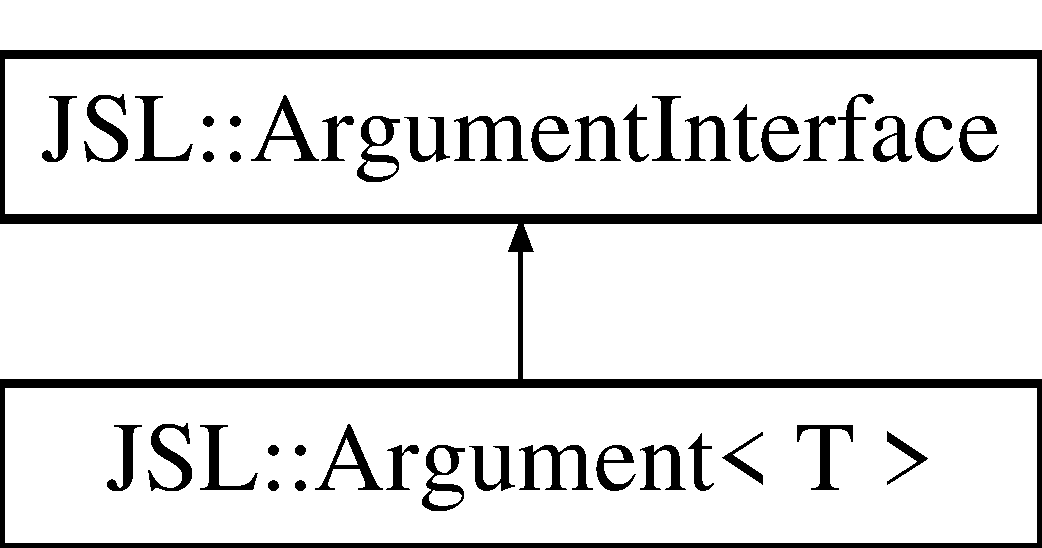
\includegraphics[height=2.000000cm]{classJSL_1_1Argument}
\end{center}
\end{figure}
\subsection*{Public Member Functions}
\begin{DoxyCompactItemize}
\item 
\hyperlink{classJSL_1_1Argument_ab438509a3c030516de72f3f493295bd5}{Argument} ()
\begin{DoxyCompactList}\small\item\em Default constructor. \end{DoxyCompactList}\item 
\hyperlink{classJSL_1_1Argument_ab07e7981db832cce30f534c67f6491f4}{Argument} (std\+::string trigger)
\begin{DoxyCompactList}\small\item\em Constructor initialising the \hyperlink{classJSL_1_1ArgumentInterface_afa2d1f96c4971070d3de5824f297312f}{Trigger\+String}. Value is set to uninitialised memory of the Template type. \end{DoxyCompactList}\item 
\hyperlink{classJSL_1_1Argument_a2511f7c98ee2b0b59650f468341b8747}{Argument} (T default\+Value, std\+::string trigger)
\begin{DoxyCompactList}\small\item\em Constructor which initialises the \hyperlink{classJSL_1_1ArgumentInterface_afa2d1f96c4971070d3de5824f297312f}{Trigger\+String} and \hyperlink{classJSL_1_1Argument_a83ada5bfa412192f76dd4290f679defd}{Value} members. \end{DoxyCompactList}\item 
\hyperlink{classJSL_1_1Argument_a4d187d2fb658021866b173987b920ab4}{Argument} (T default\+Value, std\+::string trigger, int argc, char $\ast$argv\mbox{[}$\,$\mbox{]})
\begin{DoxyCompactList}\small\item\em Constructor which initialises as per \hyperlink{classJSL_1_1Argument_a2511f7c98ee2b0b59650f468341b8747}{Argument(\+T default\+Value, std\+::string trigger)}, but which also immediately calls \hyperlink{classJSL_1_1Argument_aa2b18bb35e90f91e224a06d60835053a}{List\+Parse()} to check for assignment. \end{DoxyCompactList}\item 
\hyperlink{classJSL_1_1Argument_a83799e9089f88d7e6cf30990fae42610}{Argument} (T default\+Value, std\+::string trigger, std\+::string config\+File, char config\+Delimiter)
\begin{DoxyCompactList}\small\item\em Constructor which initialises as per \hyperlink{classJSL_1_1Argument_a2511f7c98ee2b0b59650f468341b8747}{Argument(\+T default\+Value, std\+::string trigger)}, but which also immediately calls \hyperlink{classJSL_1_1Argument_aa626ff37dbebaf0501614dc625a76383}{Configure()} to check for assignment. \end{DoxyCompactList}\item 
void \hyperlink{classJSL_1_1Argument_aa626ff37dbebaf0501614dc625a76383}{Configure} (std\+::string config\+File, char config\+Delimiter)
\begin{DoxyCompactList}\small\item\em Iterate through a configuration file, extracting Name/\+Value pairs and calling \hyperlink{classJSL_1_1Argument_a8984e7ce23155259d90a3e98170f36e0}{Parse()} in them. Each Name/\+Value pair should be on a new line in the file, and separated by the {\itshape config\+Delimiter}. \end{DoxyCompactList}\item 
void \hyperlink{classJSL_1_1Argument_aa2b18bb35e90f91e224a06d60835053a}{List\+Parse} (int argc, char $\ast$argv\mbox{[}$\,$\mbox{]})
\begin{DoxyCompactList}\small\item\em Iterate through the provided commandline args, extracting Name/\+Value pairs and calling \hyperlink{classJSL_1_1Argument_a8984e7ce23155259d90a3e98170f36e0}{Parse()} on them. \end{DoxyCompactList}\item 
void \hyperlink{classJSL_1_1Argument_a8984e7ce23155259d90a3e98170f36e0}{Parse} (char $\ast$name, char $\ast$value)
\begin{DoxyCompactList}\small\item\em Checks if the Name matches the Trigger\+String. For a successful match, Name must be prefaced by one more dash than found in Trigger\+String. \end{DoxyCompactList}\item 
\hyperlink{classJSL_1_1Argument_a965bc0dfdce6e03380605af313f8c880}{operator T} ()
\begin{DoxyCompactList}\small\item\em Allow the \hyperlink{classJSL_1_1Argument}{Argument} object to be implicitly casted into the value of \hyperlink{classJSL_1_1Argument_a83ada5bfa412192f76dd4290f679defd}{Value}, and hence treated as an object of the templated type. \end{DoxyCompactList}\end{DoxyCompactItemize}
\subsection*{Data Fields}
\begin{DoxyCompactItemize}
\item 
T \hyperlink{classJSL_1_1Argument_a83ada5bfa412192f76dd4290f679defd}{Value}
\begin{DoxyCompactList}\small\item\em The current value of the argument. \end{DoxyCompactList}\end{DoxyCompactItemize}
\subsection*{Private Member Functions}
\begin{DoxyCompactItemize}
\item 
void \hyperlink{classJSL_1_1Argument_a8614eb66f807132c4323847e05e666c4}{Check\+For\+Invalid\+Triggers} ()
\begin{DoxyCompactList}\small\item\em Some Triggers are disallowed -\/ they usually are protected names such as \char`\"{}help\char`\"{}, though other properties may trigger this funciton to throw an error. \end{DoxyCompactList}\item 
virtual void \hyperlink{classJSL_1_1Argument_ac77530598054943c996dbb5fb677b844}{Assign\+Value} (const char $\ast$value)
\begin{DoxyCompactList}\small\item\em Virtual override for template-\/specific Assign\+Value calls. Most template types will require a custom handler to convert value into the chosen template type -- some default ones are provided below. \end{DoxyCompactList}\item 
{\footnotesize template$<$$>$ }\\void \hyperlink{classJSL_1_1Argument_a6e8fe8e7cca2aeffe23f6fbadb88d4c8}{Assign\+Value} (const char $\ast$value)
\begin{DoxyCompactList}\small\item\em Override of the \hyperlink{classJSL_1_1Argument_ac77530598054943c996dbb5fb677b844}{Assign\+Value()} function for Argument$<$double$>$ objects. Throws an error if the value is a non-\/integer, to prevent silent casting/truncation. \end{DoxyCompactList}\item 
{\footnotesize template$<$$>$ }\\void \hyperlink{classJSL_1_1Argument_a059e7c6f1d9232a93cf725510fe2db27}{Assign\+Value} (const char $\ast$value)
\begin{DoxyCompactList}\small\item\em Override of the \hyperlink{classJSL_1_1Argument_ac77530598054943c996dbb5fb677b844}{Assign\+Value()} function for Argument$<$double$>$ objects. \end{DoxyCompactList}\item 
{\footnotesize template$<$$>$ }\\void \hyperlink{classJSL_1_1Argument_af5ccee16ba3403ef62d4bec9d380c762}{Assign\+Value} (const char $\ast$value)
\begin{DoxyCompactList}\small\item\em Override of the \hyperlink{classJSL_1_1Argument_ac77530598054943c996dbb5fb677b844}{Assign\+Value()} function for \hyperlink{classJSL_1_1Argument_ab438509a3c030516de72f3f493295bd5}{Argument$<$std\+::string$>$} objects. \end{DoxyCompactList}\item 
{\footnotesize template$<$$>$ }\\void \hyperlink{classJSL_1_1Argument_a0831822da0a2da47daa07d2e51b87d2a}{Assign\+Value} (const char $\ast$value)
\begin{DoxyCompactList}\small\item\em Override of the \hyperlink{classJSL_1_1Argument_ac77530598054943c996dbb5fb677b844}{Assign\+Value()} function for Argument$<$bool$>$ objects. Accepts only 0/1 as valid bool-\/strings. \end{DoxyCompactList}\end{DoxyCompactItemize}
\subsection*{Additional Inherited Members}


\subsection{Detailed Description}
\subsubsection*{template$<$class T$>$\newline
class J\+S\+L\+::\+Argument$<$ T $>$}

A class which allows arbitrary template parameters to be read in as command-\/line arguments or from a configuraiton file using a Name/\+Value pair system. Upon construction, the \hyperlink{classJSL_1_1Argument_a83ada5bfa412192f76dd4290f679defd}{Value} parameter takes the default value (if provided), until it is overriden by a successful argument/\hyperlink{classJSL_1_1ArgumentInterface_afa2d1f96c4971070d3de5824f297312f}{Trigger\+String} match. 

\subsection{Constructor \& Destructor Documentation}
\mbox{\Hypertarget{classJSL_1_1Argument_ab438509a3c030516de72f3f493295bd5}\label{classJSL_1_1Argument_ab438509a3c030516de72f3f493295bd5}} 
\index{J\+S\+L\+::\+Argument@{J\+S\+L\+::\+Argument}!Argument@{Argument}}
\index{Argument@{Argument}!J\+S\+L\+::\+Argument@{J\+S\+L\+::\+Argument}}
\subsubsection{\texorpdfstring{Argument()}{Argument()}\hspace{0.1cm}{\footnotesize\ttfamily [1/5]}}
{\footnotesize\ttfamily template$<$class T$>$ \\
\hyperlink{classJSL_1_1Argument}{J\+S\+L\+::\+Argument}$<$ T $>$\+::\hyperlink{classJSL_1_1Argument}{Argument} (\begin{DoxyParamCaption}{ }\end{DoxyParamCaption})\hspace{0.3cm}{\ttfamily [inline]}}



Default constructor. 

\mbox{\Hypertarget{classJSL_1_1Argument_ab07e7981db832cce30f534c67f6491f4}\label{classJSL_1_1Argument_ab07e7981db832cce30f534c67f6491f4}} 
\index{J\+S\+L\+::\+Argument@{J\+S\+L\+::\+Argument}!Argument@{Argument}}
\index{Argument@{Argument}!J\+S\+L\+::\+Argument@{J\+S\+L\+::\+Argument}}
\subsubsection{\texorpdfstring{Argument()}{Argument()}\hspace{0.1cm}{\footnotesize\ttfamily [2/5]}}
{\footnotesize\ttfamily template$<$class T$>$ \\
\hyperlink{classJSL_1_1Argument}{J\+S\+L\+::\+Argument}$<$ T $>$\+::\hyperlink{classJSL_1_1Argument}{Argument} (\begin{DoxyParamCaption}\item[{std\+::string}]{trigger }\end{DoxyParamCaption})\hspace{0.3cm}{\ttfamily [inline]}}



Constructor initialising the \hyperlink{classJSL_1_1ArgumentInterface_afa2d1f96c4971070d3de5824f297312f}{Trigger\+String}. Value is set to uninitialised memory of the Template type. 


\begin{DoxyParams}{Parameters}
{\em trigger} & The value of \hyperlink{classJSL_1_1ArgumentInterface_afa2d1f96c4971070d3de5824f297312f}{Trigger\+String}, and the \char`\"{}name\char`\"{} of this parameter \\
\hline
\end{DoxyParams}
\mbox{\Hypertarget{classJSL_1_1Argument_a2511f7c98ee2b0b59650f468341b8747}\label{classJSL_1_1Argument_a2511f7c98ee2b0b59650f468341b8747}} 
\index{J\+S\+L\+::\+Argument@{J\+S\+L\+::\+Argument}!Argument@{Argument}}
\index{Argument@{Argument}!J\+S\+L\+::\+Argument@{J\+S\+L\+::\+Argument}}
\subsubsection{\texorpdfstring{Argument()}{Argument()}\hspace{0.1cm}{\footnotesize\ttfamily [3/5]}}
{\footnotesize\ttfamily template$<$class T$>$ \\
\hyperlink{classJSL_1_1Argument}{J\+S\+L\+::\+Argument}$<$ T $>$\+::\hyperlink{classJSL_1_1Argument}{Argument} (\begin{DoxyParamCaption}\item[{T}]{default\+Value,  }\item[{std\+::string}]{trigger }\end{DoxyParamCaption})\hspace{0.3cm}{\ttfamily [inline]}}



Constructor which initialises the \hyperlink{classJSL_1_1ArgumentInterface_afa2d1f96c4971070d3de5824f297312f}{Trigger\+String} and \hyperlink{classJSL_1_1Argument_a83ada5bfa412192f76dd4290f679defd}{Value} members. 


\begin{DoxyParams}{Parameters}
{\em default\+Value} & The initialisation value of \hyperlink{classJSL_1_1Argument_a83ada5bfa412192f76dd4290f679defd}{Value} -\/ overridden if \hyperlink{classJSL_1_1Argument_a8984e7ce23155259d90a3e98170f36e0}{Parse()} is called. \\
\hline
{\em trigger} & The value of \hyperlink{classJSL_1_1ArgumentInterface_afa2d1f96c4971070d3de5824f297312f}{Trigger\+String}, and the \char`\"{}name\char`\"{} of this parameter \\
\hline
\end{DoxyParams}
\mbox{\Hypertarget{classJSL_1_1Argument_a4d187d2fb658021866b173987b920ab4}\label{classJSL_1_1Argument_a4d187d2fb658021866b173987b920ab4}} 
\index{J\+S\+L\+::\+Argument@{J\+S\+L\+::\+Argument}!Argument@{Argument}}
\index{Argument@{Argument}!J\+S\+L\+::\+Argument@{J\+S\+L\+::\+Argument}}
\subsubsection{\texorpdfstring{Argument()}{Argument()}\hspace{0.1cm}{\footnotesize\ttfamily [4/5]}}
{\footnotesize\ttfamily template$<$class T$>$ \\
\hyperlink{classJSL_1_1Argument}{J\+S\+L\+::\+Argument}$<$ T $>$\+::\hyperlink{classJSL_1_1Argument}{Argument} (\begin{DoxyParamCaption}\item[{T}]{default\+Value,  }\item[{std\+::string}]{trigger,  }\item[{int}]{argc,  }\item[{char $\ast$}]{argv\mbox{[}$\,$\mbox{]} }\end{DoxyParamCaption})\hspace{0.3cm}{\ttfamily [inline]}}



Constructor which initialises as per \hyperlink{classJSL_1_1Argument_a2511f7c98ee2b0b59650f468341b8747}{Argument(\+T default\+Value, std\+::string trigger)}, but which also immediately calls \hyperlink{classJSL_1_1Argument_aa2b18bb35e90f91e224a06d60835053a}{List\+Parse()} to check for assignment. 


\begin{DoxyParams}{Parameters}
{\em default\+Value} & The initialisation value of \hyperlink{classJSL_1_1Argument_a83ada5bfa412192f76dd4290f679defd}{Value} -\/ overridden if \hyperlink{classJSL_1_1Argument_a8984e7ce23155259d90a3e98170f36e0}{Parse()} is called. \\
\hline
{\em trigger} & The value of \hyperlink{classJSL_1_1ArgumentInterface_afa2d1f96c4971070d3de5824f297312f}{Trigger\+String}, and the \char`\"{}name\char`\"{} of this parameter \\
\hline
{\em argc} & The number of commandline arguments \\
\hline
{\em argv\mbox{[}$\,$\mbox{]}} & the command line list \\
\hline
\end{DoxyParams}
\mbox{\Hypertarget{classJSL_1_1Argument_a83799e9089f88d7e6cf30990fae42610}\label{classJSL_1_1Argument_a83799e9089f88d7e6cf30990fae42610}} 
\index{J\+S\+L\+::\+Argument@{J\+S\+L\+::\+Argument}!Argument@{Argument}}
\index{Argument@{Argument}!J\+S\+L\+::\+Argument@{J\+S\+L\+::\+Argument}}
\subsubsection{\texorpdfstring{Argument()}{Argument()}\hspace{0.1cm}{\footnotesize\ttfamily [5/5]}}
{\footnotesize\ttfamily template$<$class T$>$ \\
\hyperlink{classJSL_1_1Argument}{J\+S\+L\+::\+Argument}$<$ T $>$\+::\hyperlink{classJSL_1_1Argument}{Argument} (\begin{DoxyParamCaption}\item[{T}]{default\+Value,  }\item[{std\+::string}]{trigger,  }\item[{std\+::string}]{config\+File,  }\item[{char}]{config\+Delimiter }\end{DoxyParamCaption})\hspace{0.3cm}{\ttfamily [inline]}}



Constructor which initialises as per \hyperlink{classJSL_1_1Argument_a2511f7c98ee2b0b59650f468341b8747}{Argument(\+T default\+Value, std\+::string trigger)}, but which also immediately calls \hyperlink{classJSL_1_1Argument_aa626ff37dbebaf0501614dc625a76383}{Configure()} to check for assignment. 


\begin{DoxyParams}{Parameters}
{\em default\+Value} & The initialisation value of \hyperlink{classJSL_1_1Argument_a83ada5bfa412192f76dd4290f679defd}{Value} -\/ overridden if \hyperlink{classJSL_1_1Argument_a8984e7ce23155259d90a3e98170f36e0}{Parse()} is called. \\
\hline
{\em trigger} & The value of \hyperlink{classJSL_1_1ArgumentInterface_afa2d1f96c4971070d3de5824f297312f}{Trigger\+String}, and the \char`\"{}name\char`\"{} of this parameter \\
\hline
{\em config\+File} & The path to the file to open and parse for configuration data \\
\hline
{\em config\+Delimiter} & The delimiter used to separate Name/\+Value pairs in the cofiguration file \\
\hline
\end{DoxyParams}


\subsection{Member Function Documentation}
\mbox{\Hypertarget{classJSL_1_1Argument_ac77530598054943c996dbb5fb677b844}\label{classJSL_1_1Argument_ac77530598054943c996dbb5fb677b844}} 
\index{J\+S\+L\+::\+Argument@{J\+S\+L\+::\+Argument}!Assign\+Value@{Assign\+Value}}
\index{Assign\+Value@{Assign\+Value}!J\+S\+L\+::\+Argument@{J\+S\+L\+::\+Argument}}
\subsubsection{\texorpdfstring{Assign\+Value()}{AssignValue()}\hspace{0.1cm}{\footnotesize\ttfamily [1/5]}}
{\footnotesize\ttfamily template$<$class T$>$ \\
virtual void \hyperlink{classJSL_1_1Argument}{J\+S\+L\+::\+Argument}$<$ T $>$\+::Assign\+Value (\begin{DoxyParamCaption}\item[{const char $\ast$}]{value }\end{DoxyParamCaption})\hspace{0.3cm}{\ttfamily [inline]}, {\ttfamily [private]}, {\ttfamily [virtual]}}



Virtual override for template-\/specific Assign\+Value calls. Most template types will require a custom handler to convert value into the chosen template type -- some default ones are provided below. 

\mbox{\Hypertarget{classJSL_1_1Argument_a6e8fe8e7cca2aeffe23f6fbadb88d4c8}\label{classJSL_1_1Argument_a6e8fe8e7cca2aeffe23f6fbadb88d4c8}} 
\index{J\+S\+L\+::\+Argument@{J\+S\+L\+::\+Argument}!Assign\+Value@{Assign\+Value}}
\index{Assign\+Value@{Assign\+Value}!J\+S\+L\+::\+Argument@{J\+S\+L\+::\+Argument}}
\subsubsection{\texorpdfstring{Assign\+Value()}{AssignValue()}\hspace{0.1cm}{\footnotesize\ttfamily [2/5]}}
{\footnotesize\ttfamily template$<$$>$ \\
void \hyperlink{classJSL_1_1Argument}{J\+S\+L\+::\+Argument}$<$ int $>$\+::Assign\+Value (\begin{DoxyParamCaption}\item[{const char $\ast$}]{value }\end{DoxyParamCaption})\hspace{0.3cm}{\ttfamily [inline]}, {\ttfamily [private]}}



Override of the \hyperlink{classJSL_1_1Argument_ac77530598054943c996dbb5fb677b844}{Assign\+Value()} function for Argument$<$double$>$ objects. Throws an error if the value is a non-\/integer, to prevent silent casting/truncation. 

\mbox{\Hypertarget{classJSL_1_1Argument_a059e7c6f1d9232a93cf725510fe2db27}\label{classJSL_1_1Argument_a059e7c6f1d9232a93cf725510fe2db27}} 
\index{J\+S\+L\+::\+Argument@{J\+S\+L\+::\+Argument}!Assign\+Value@{Assign\+Value}}
\index{Assign\+Value@{Assign\+Value}!J\+S\+L\+::\+Argument@{J\+S\+L\+::\+Argument}}
\subsubsection{\texorpdfstring{Assign\+Value()}{AssignValue()}\hspace{0.1cm}{\footnotesize\ttfamily [3/5]}}
{\footnotesize\ttfamily template$<$$>$ \\
void \hyperlink{classJSL_1_1Argument}{J\+S\+L\+::\+Argument}$<$ double $>$\+::Assign\+Value (\begin{DoxyParamCaption}\item[{const char $\ast$}]{value }\end{DoxyParamCaption})\hspace{0.3cm}{\ttfamily [inline]}, {\ttfamily [private]}}



Override of the \hyperlink{classJSL_1_1Argument_ac77530598054943c996dbb5fb677b844}{Assign\+Value()} function for Argument$<$double$>$ objects. 

\mbox{\Hypertarget{classJSL_1_1Argument_af5ccee16ba3403ef62d4bec9d380c762}\label{classJSL_1_1Argument_af5ccee16ba3403ef62d4bec9d380c762}} 
\index{J\+S\+L\+::\+Argument@{J\+S\+L\+::\+Argument}!Assign\+Value@{Assign\+Value}}
\index{Assign\+Value@{Assign\+Value}!J\+S\+L\+::\+Argument@{J\+S\+L\+::\+Argument}}
\subsubsection{\texorpdfstring{Assign\+Value()}{AssignValue()}\hspace{0.1cm}{\footnotesize\ttfamily [4/5]}}
{\footnotesize\ttfamily template$<$$>$ \\
void \hyperlink{classJSL_1_1Argument}{J\+S\+L\+::\+Argument}$<$ std\+::string $>$\+::Assign\+Value (\begin{DoxyParamCaption}\item[{const char $\ast$}]{value }\end{DoxyParamCaption})\hspace{0.3cm}{\ttfamily [inline]}, {\ttfamily [private]}}



Override of the \hyperlink{classJSL_1_1Argument_ac77530598054943c996dbb5fb677b844}{Assign\+Value()} function for \hyperlink{classJSL_1_1Argument_ab438509a3c030516de72f3f493295bd5}{Argument$<$std\+::string$>$} objects. 

\mbox{\Hypertarget{classJSL_1_1Argument_a0831822da0a2da47daa07d2e51b87d2a}\label{classJSL_1_1Argument_a0831822da0a2da47daa07d2e51b87d2a}} 
\index{J\+S\+L\+::\+Argument@{J\+S\+L\+::\+Argument}!Assign\+Value@{Assign\+Value}}
\index{Assign\+Value@{Assign\+Value}!J\+S\+L\+::\+Argument@{J\+S\+L\+::\+Argument}}
\subsubsection{\texorpdfstring{Assign\+Value()}{AssignValue()}\hspace{0.1cm}{\footnotesize\ttfamily [5/5]}}
{\footnotesize\ttfamily template$<$$>$ \\
void \hyperlink{classJSL_1_1Argument}{J\+S\+L\+::\+Argument}$<$ bool $>$\+::Assign\+Value (\begin{DoxyParamCaption}\item[{const char $\ast$}]{value }\end{DoxyParamCaption})\hspace{0.3cm}{\ttfamily [inline]}, {\ttfamily [private]}}



Override of the \hyperlink{classJSL_1_1Argument_ac77530598054943c996dbb5fb677b844}{Assign\+Value()} function for Argument$<$bool$>$ objects. Accepts only 0/1 as valid bool-\/strings. 

\mbox{\Hypertarget{classJSL_1_1Argument_a8614eb66f807132c4323847e05e666c4}\label{classJSL_1_1Argument_a8614eb66f807132c4323847e05e666c4}} 
\index{J\+S\+L\+::\+Argument@{J\+S\+L\+::\+Argument}!Check\+For\+Invalid\+Triggers@{Check\+For\+Invalid\+Triggers}}
\index{Check\+For\+Invalid\+Triggers@{Check\+For\+Invalid\+Triggers}!J\+S\+L\+::\+Argument@{J\+S\+L\+::\+Argument}}
\subsubsection{\texorpdfstring{Check\+For\+Invalid\+Triggers()}{CheckForInvalidTriggers()}}
{\footnotesize\ttfamily template$<$class T$>$ \\
void \hyperlink{classJSL_1_1Argument}{J\+S\+L\+::\+Argument}$<$ T $>$\+::Check\+For\+Invalid\+Triggers (\begin{DoxyParamCaption}{ }\end{DoxyParamCaption})\hspace{0.3cm}{\ttfamily [inline]}, {\ttfamily [private]}}



Some Triggers are disallowed -\/ they usually are protected names such as \char`\"{}help\char`\"{}, though other properties may trigger this funciton to throw an error. 

\mbox{\Hypertarget{classJSL_1_1Argument_aa626ff37dbebaf0501614dc625a76383}\label{classJSL_1_1Argument_aa626ff37dbebaf0501614dc625a76383}} 
\index{J\+S\+L\+::\+Argument@{J\+S\+L\+::\+Argument}!Configure@{Configure}}
\index{Configure@{Configure}!J\+S\+L\+::\+Argument@{J\+S\+L\+::\+Argument}}
\subsubsection{\texorpdfstring{Configure()}{Configure()}}
{\footnotesize\ttfamily template$<$class T$>$ \\
void \hyperlink{classJSL_1_1Argument}{J\+S\+L\+::\+Argument}$<$ T $>$\+::Configure (\begin{DoxyParamCaption}\item[{std\+::string}]{config\+File,  }\item[{char}]{config\+Delimiter }\end{DoxyParamCaption})\hspace{0.3cm}{\ttfamily [inline]}, {\ttfamily [virtual]}}



Iterate through a configuration file, extracting Name/\+Value pairs and calling \hyperlink{classJSL_1_1Argument_a8984e7ce23155259d90a3e98170f36e0}{Parse()} in them. Each Name/\+Value pair should be on a new line in the file, and separated by the {\itshape config\+Delimiter}. 


\begin{DoxyParams}{Parameters}
{\em config\+File} & The path to the file to open and parse for configuration data \\
\hline
{\em config\+Delimiter} & The delimiter used to separate Name/\+Value pairs in the cofiguration file \\
\hline
\end{DoxyParams}


Reimplemented from \hyperlink{classJSL_1_1ArgumentInterface_aac7c3106f99c407e625b9bc6a6c8c446}{J\+S\+L\+::\+Argument\+Interface}.

\mbox{\Hypertarget{classJSL_1_1Argument_aa2b18bb35e90f91e224a06d60835053a}\label{classJSL_1_1Argument_aa2b18bb35e90f91e224a06d60835053a}} 
\index{J\+S\+L\+::\+Argument@{J\+S\+L\+::\+Argument}!List\+Parse@{List\+Parse}}
\index{List\+Parse@{List\+Parse}!J\+S\+L\+::\+Argument@{J\+S\+L\+::\+Argument}}
\subsubsection{\texorpdfstring{List\+Parse()}{ListParse()}}
{\footnotesize\ttfamily template$<$class T$>$ \\
void \hyperlink{classJSL_1_1Argument}{J\+S\+L\+::\+Argument}$<$ T $>$\+::List\+Parse (\begin{DoxyParamCaption}\item[{int}]{argc,  }\item[{char $\ast$}]{argv\mbox{[}$\,$\mbox{]} }\end{DoxyParamCaption})\hspace{0.3cm}{\ttfamily [inline]}, {\ttfamily [virtual]}}



Iterate through the provided commandline args, extracting Name/\+Value pairs and calling \hyperlink{classJSL_1_1Argument_a8984e7ce23155259d90a3e98170f36e0}{Parse()} on them. 


\begin{DoxyParams}{Parameters}
{\em argc} & The number of arguments passed to the program \\
\hline
{\em argv\mbox{[}$\,$\mbox{]}} & The argument list (argv\mbox{[}0\mbox{]} is assumed to be the the name of the program, and is ignored) \\
\hline
\end{DoxyParams}


Reimplemented from \hyperlink{classJSL_1_1ArgumentInterface_a256b5bd88b5f6638353f108c48f3ee65}{J\+S\+L\+::\+Argument\+Interface}.

\mbox{\Hypertarget{classJSL_1_1Argument_a965bc0dfdce6e03380605af313f8c880}\label{classJSL_1_1Argument_a965bc0dfdce6e03380605af313f8c880}} 
\index{J\+S\+L\+::\+Argument@{J\+S\+L\+::\+Argument}!operator T@{operator T}}
\index{operator T@{operator T}!J\+S\+L\+::\+Argument@{J\+S\+L\+::\+Argument}}
\subsubsection{\texorpdfstring{operator T()}{operator T()}}
{\footnotesize\ttfamily template$<$class T$>$ \\
\hyperlink{classJSL_1_1Argument}{J\+S\+L\+::\+Argument}$<$ T $>$\+::operator T (\begin{DoxyParamCaption}{ }\end{DoxyParamCaption})\hspace{0.3cm}{\ttfamily [inline]}}



Allow the \hyperlink{classJSL_1_1Argument}{Argument} object to be implicitly casted into the value of \hyperlink{classJSL_1_1Argument_a83ada5bfa412192f76dd4290f679defd}{Value}, and hence treated as an object of the templated type. 

\mbox{\Hypertarget{classJSL_1_1Argument_a8984e7ce23155259d90a3e98170f36e0}\label{classJSL_1_1Argument_a8984e7ce23155259d90a3e98170f36e0}} 
\index{J\+S\+L\+::\+Argument@{J\+S\+L\+::\+Argument}!Parse@{Parse}}
\index{Parse@{Parse}!J\+S\+L\+::\+Argument@{J\+S\+L\+::\+Argument}}
\subsubsection{\texorpdfstring{Parse()}{Parse()}}
{\footnotesize\ttfamily template$<$class T$>$ \\
void \hyperlink{classJSL_1_1Argument}{J\+S\+L\+::\+Argument}$<$ T $>$\+::Parse (\begin{DoxyParamCaption}\item[{char $\ast$}]{name,  }\item[{char $\ast$}]{value }\end{DoxyParamCaption})\hspace{0.3cm}{\ttfamily [inline]}, {\ttfamily [virtual]}}



Checks if the Name matches the Trigger\+String. For a successful match, Name must be prefaced by one more dash than found in Trigger\+String. 


\begin{DoxyParams}{Parameters}
{\em name} & The name-\/string of the Name/\+Value pair\\
\hline
{\em value} & The value-\/string of the Name/\+Value pair. \\
\hline
\end{DoxyParams}


Reimplemented from \hyperlink{classJSL_1_1ArgumentInterface_a28b487f7a4fa6e721ed6629abe2073f2}{J\+S\+L\+::\+Argument\+Interface}.



\subsection{Field Documentation}
\mbox{\Hypertarget{classJSL_1_1Argument_a83ada5bfa412192f76dd4290f679defd}\label{classJSL_1_1Argument_a83ada5bfa412192f76dd4290f679defd}} 
\index{J\+S\+L\+::\+Argument@{J\+S\+L\+::\+Argument}!Value@{Value}}
\index{Value@{Value}!J\+S\+L\+::\+Argument@{J\+S\+L\+::\+Argument}}
\subsubsection{\texorpdfstring{Value}{Value}}
{\footnotesize\ttfamily template$<$class T$>$ \\
T \hyperlink{classJSL_1_1Argument}{J\+S\+L\+::\+Argument}$<$ T $>$\+::Value}



The current value of the argument. 



The documentation for this class was generated from the following file\+:\begin{DoxyCompactItemize}
\item 
/home/f/fraserj/\+Documents/\+Work/\+Q\+Dynamics/lib/\+J\+S\+L/\+Command\+Args/\hyperlink{Argument_8h}{Argument.\+h}\end{DoxyCompactItemize}

\hypertarget{classJSL_1_1ArgumentInterface}{}\doxysection{J\+SL\+::Argument\+Interface Class Reference}
\label{classJSL_1_1ArgumentInterface}\index{JSL::ArgumentInterface@{JSL::ArgumentInterface}}


{\ttfamily \#include $<$Argument.\+h$>$}

Inheritance diagram for J\+SL\+::Argument\+Interface\+:\begin{figure}[H]
\begin{center}
\leavevmode
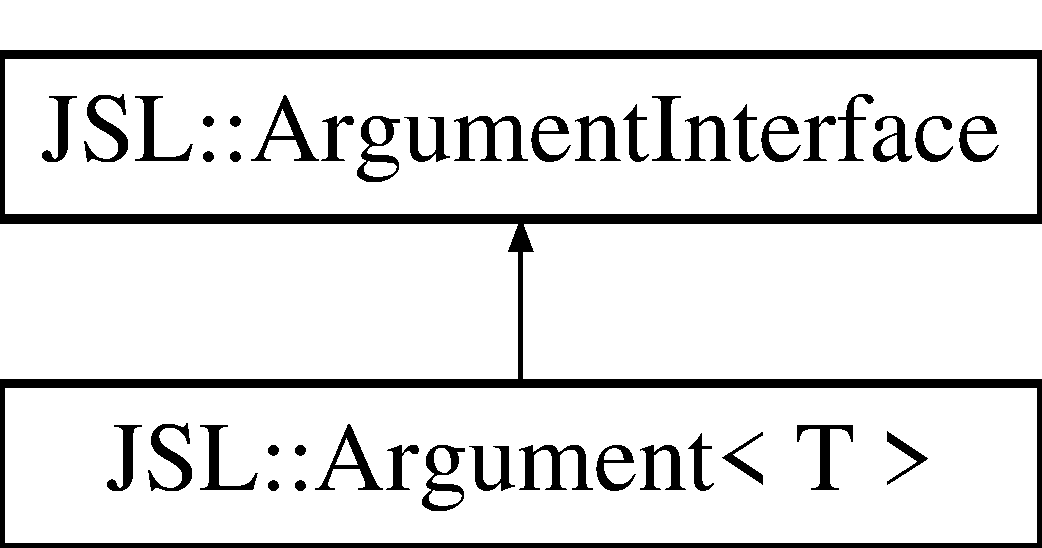
\includegraphics[height=2.000000cm]{classJSL_1_1ArgumentInterface}
\end{center}
\end{figure}
\doxysubsection*{Public Member Functions}
\begin{DoxyCompactItemize}
\item 
virtual void \mbox{\hyperlink{classJSL_1_1ArgumentInterface_a28b487f7a4fa6e721ed6629abe2073f2}{Parse}} (char $\ast$name, char $\ast$value)
\begin{DoxyCompactList}\small\item\em Virtual alias for \mbox{\hyperlink{classJSL_1_1Argument_a8984e7ce23155259d90a3e98170f36e0}{Argument\+::\+Parse()}} \end{DoxyCompactList}\item 
virtual void \mbox{\hyperlink{classJSL_1_1ArgumentInterface_a256b5bd88b5f6638353f108c48f3ee65}{List\+Parse}} (int argc, char $\ast$argv\mbox{[}$\,$\mbox{]})
\begin{DoxyCompactList}\small\item\em Virtual alias for \mbox{\hyperlink{classJSL_1_1Argument_aa2b18bb35e90f91e224a06d60835053a}{Argument\+::\+List\+Parse()}} \end{DoxyCompactList}\item 
virtual void \mbox{\hyperlink{classJSL_1_1ArgumentInterface_aac7c3106f99c407e625b9bc6a6c8c446}{Configure}} (std\+::string config\+File, char config\+Delimiter)
\begin{DoxyCompactList}\small\item\em Virtual alias for \mbox{\hyperlink{classJSL_1_1Argument_aa626ff37dbebaf0501614dc625a76383}{Argument\+::\+Configure()}} \end{DoxyCompactList}\end{DoxyCompactItemize}
\doxysubsection*{Protected Attributes}
\begin{DoxyCompactItemize}
\item 
std\+::string \mbox{\hyperlink{classJSL_1_1ArgumentInterface_afa2d1f96c4971070d3de5824f297312f}{Trigger\+String}}
\begin{DoxyCompactList}\small\item\em The chosen \char`\"{}\+Name\char`\"{} of the \mbox{\hyperlink{classJSL_1_1Argument}{Argument}} -\/ the string which will trigger the \mbox{\hyperlink{classJSL_1_1ArgumentInterface_a28b487f7a4fa6e721ed6629abe2073f2}{Parse()}} function to write in the passed value. \end{DoxyCompactList}\end{DoxyCompactItemize}


\doxysubsection{Detailed Description}
A wrapper class for all \mbox{\hyperlink{classJSL_1_1Argument}{Argument}} objects, enabling heterogenous argument lists etc. to be constructed. ~\newline
 Contains the virtual methods common to all objects. All \mbox{\hyperlink{classJSL_1_1Argument}{Argument}} objects are assumed to take name-\/value pairs, with the associated name indicated by the \mbox{\hyperlink{classJSL_1_1ArgumentInterface_afa2d1f96c4971070d3de5824f297312f}{Trigger\+String}} 

\doxysubsection{Member Function Documentation}
\mbox{\Hypertarget{classJSL_1_1ArgumentInterface_aac7c3106f99c407e625b9bc6a6c8c446}\label{classJSL_1_1ArgumentInterface_aac7c3106f99c407e625b9bc6a6c8c446}} 
\index{JSL::ArgumentInterface@{JSL::ArgumentInterface}!Configure@{Configure}}
\index{Configure@{Configure}!JSL::ArgumentInterface@{JSL::ArgumentInterface}}
\doxysubsubsection{\texorpdfstring{Configure()}{Configure()}}
{\footnotesize\ttfamily virtual void J\+S\+L\+::\+Argument\+Interface\+::\+Configure (\begin{DoxyParamCaption}\item[{std\+::string}]{config\+File,  }\item[{char}]{config\+Delimiter }\end{DoxyParamCaption})\hspace{0.3cm}{\ttfamily [inline]}, {\ttfamily [virtual]}}



Virtual alias for \mbox{\hyperlink{classJSL_1_1Argument_aa626ff37dbebaf0501614dc625a76383}{Argument\+::\+Configure()}} 



Reimplemented in \mbox{\hyperlink{classJSL_1_1Argument_aa626ff37dbebaf0501614dc625a76383}{J\+S\+L\+::\+Argument$<$ T $>$}}.

\mbox{\Hypertarget{classJSL_1_1ArgumentInterface_a256b5bd88b5f6638353f108c48f3ee65}\label{classJSL_1_1ArgumentInterface_a256b5bd88b5f6638353f108c48f3ee65}} 
\index{JSL::ArgumentInterface@{JSL::ArgumentInterface}!ListParse@{ListParse}}
\index{ListParse@{ListParse}!JSL::ArgumentInterface@{JSL::ArgumentInterface}}
\doxysubsubsection{\texorpdfstring{ListParse()}{ListParse()}}
{\footnotesize\ttfamily virtual void J\+S\+L\+::\+Argument\+Interface\+::\+List\+Parse (\begin{DoxyParamCaption}\item[{int}]{argc,  }\item[{char $\ast$}]{argv\mbox{[}$\,$\mbox{]} }\end{DoxyParamCaption})\hspace{0.3cm}{\ttfamily [inline]}, {\ttfamily [virtual]}}



Virtual alias for \mbox{\hyperlink{classJSL_1_1Argument_aa2b18bb35e90f91e224a06d60835053a}{Argument\+::\+List\+Parse()}} 



Reimplemented in \mbox{\hyperlink{classJSL_1_1Argument_aa2b18bb35e90f91e224a06d60835053a}{J\+S\+L\+::\+Argument$<$ T $>$}}.

\mbox{\Hypertarget{classJSL_1_1ArgumentInterface_a28b487f7a4fa6e721ed6629abe2073f2}\label{classJSL_1_1ArgumentInterface_a28b487f7a4fa6e721ed6629abe2073f2}} 
\index{JSL::ArgumentInterface@{JSL::ArgumentInterface}!Parse@{Parse}}
\index{Parse@{Parse}!JSL::ArgumentInterface@{JSL::ArgumentInterface}}
\doxysubsubsection{\texorpdfstring{Parse()}{Parse()}}
{\footnotesize\ttfamily virtual void J\+S\+L\+::\+Argument\+Interface\+::\+Parse (\begin{DoxyParamCaption}\item[{char $\ast$}]{name,  }\item[{char $\ast$}]{value }\end{DoxyParamCaption})\hspace{0.3cm}{\ttfamily [inline]}, {\ttfamily [virtual]}}



Virtual alias for \mbox{\hyperlink{classJSL_1_1Argument_a8984e7ce23155259d90a3e98170f36e0}{Argument\+::\+Parse()}} 



Reimplemented in \mbox{\hyperlink{classJSL_1_1Argument_a8984e7ce23155259d90a3e98170f36e0}{J\+S\+L\+::\+Argument$<$ T $>$}}.



\doxysubsection{Field Documentation}
\mbox{\Hypertarget{classJSL_1_1ArgumentInterface_afa2d1f96c4971070d3de5824f297312f}\label{classJSL_1_1ArgumentInterface_afa2d1f96c4971070d3de5824f297312f}} 
\index{JSL::ArgumentInterface@{JSL::ArgumentInterface}!TriggerString@{TriggerString}}
\index{TriggerString@{TriggerString}!JSL::ArgumentInterface@{JSL::ArgumentInterface}}
\doxysubsubsection{\texorpdfstring{TriggerString}{TriggerString}}
{\footnotesize\ttfamily std\+::string J\+S\+L\+::\+Argument\+Interface\+::\+Trigger\+String\hspace{0.3cm}{\ttfamily [protected]}}



The chosen \char`\"{}\+Name\char`\"{} of the \mbox{\hyperlink{classJSL_1_1Argument}{Argument}} -\/ the string which will trigger the \mbox{\hyperlink{classJSL_1_1ArgumentInterface_a28b487f7a4fa6e721ed6629abe2073f2}{Parse()}} function to write in the passed value. 



The documentation for this class was generated from the following file\+:\begin{DoxyCompactItemize}
\item 
/home/jack/\+Documents/\+Work/\+Q\+Dynamics/lib/\+J\+S\+L/\+Command\+Args/\mbox{\hyperlink{Argument_8h}{Argument.\+h}}\end{DoxyCompactItemize}

\hypertarget{classJSL__Testing_1_1ArgumentTest}{}\doxysection{J\+S\+L\+\_\+\+Testing\+::Argument\+Test Class Reference}
\label{classJSL__Testing_1_1ArgumentTest}\index{JSL\_Testing::ArgumentTest@{JSL\_Testing::ArgumentTest}}


{\ttfamily \#include $<$Testing\+\_\+\+Unit\+Tests.\+h$>$}

Inheritance diagram for J\+S\+L\+\_\+\+Testing\+::Argument\+Test\+:\begin{figure}[H]
\begin{center}
\leavevmode
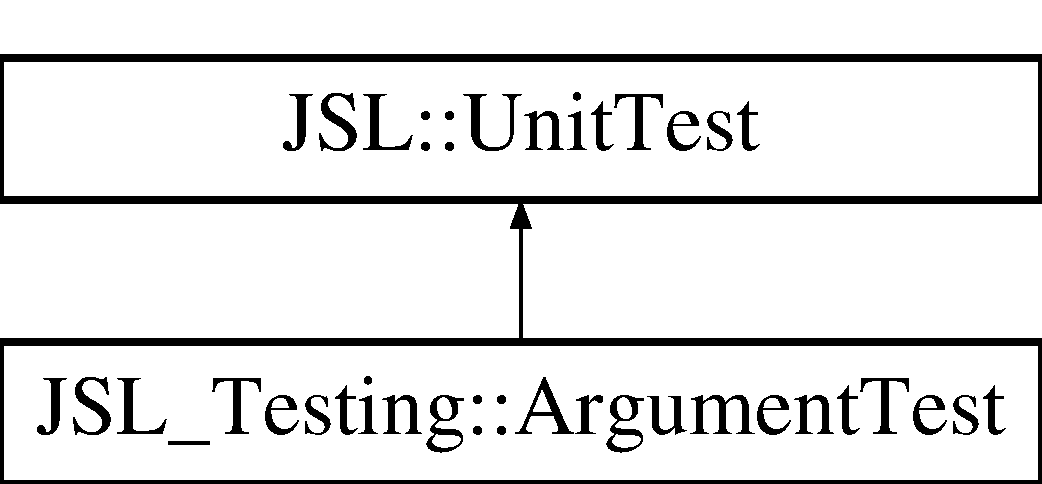
\includegraphics[height=2.000000cm]{classJSL__Testing_1_1ArgumentTest}
\end{center}
\end{figure}
\doxysubsection*{Public Member Functions}
\begin{DoxyCompactItemize}
\item 
\mbox{\hyperlink{classJSL__Testing_1_1ArgumentTest_a3d83658826bd70b33349e53a7326ae5a}{Argument\+Test}} ()
\item 
void \mbox{\hyperlink{classJSL__Testing_1_1ArgumentTest_a1c4c626d57e448da86866ef414308e97}{Run\+\_\+\+Test}} ()
\begin{DoxyCompactList}\small\item\em All children which want to take advantage of the \mbox{\hyperlink{classJSL_1_1UnitTest_aabec19b081be8a428f12e4b5e3dc2a9c}{Buffered\+Test()}} command should have the bulk of their testing within this command. \end{DoxyCompactList}\end{DoxyCompactItemize}
\doxysubsection*{Additional Inherited Members}


\doxysubsection{Constructor \& Destructor Documentation}
\mbox{\Hypertarget{classJSL__Testing_1_1ArgumentTest_a3d83658826bd70b33349e53a7326ae5a}\label{classJSL__Testing_1_1ArgumentTest_a3d83658826bd70b33349e53a7326ae5a}} 
\index{JSL\_Testing::ArgumentTest@{JSL\_Testing::ArgumentTest}!ArgumentTest@{ArgumentTest}}
\index{ArgumentTest@{ArgumentTest}!JSL\_Testing::ArgumentTest@{JSL\_Testing::ArgumentTest}}
\doxysubsubsection{\texorpdfstring{ArgumentTest()}{ArgumentTest()}}
{\footnotesize\ttfamily J\+S\+L\+\_\+\+Testing\+::\+Argument\+Test\+::\+Argument\+Test (\begin{DoxyParamCaption}{ }\end{DoxyParamCaption})\hspace{0.3cm}{\ttfamily [inline]}}



\doxysubsection{Member Function Documentation}
\mbox{\Hypertarget{classJSL__Testing_1_1ArgumentTest_a1c4c626d57e448da86866ef414308e97}\label{classJSL__Testing_1_1ArgumentTest_a1c4c626d57e448da86866ef414308e97}} 
\index{JSL\_Testing::ArgumentTest@{JSL\_Testing::ArgumentTest}!Run\_Test@{Run\_Test}}
\index{Run\_Test@{Run\_Test}!JSL\_Testing::ArgumentTest@{JSL\_Testing::ArgumentTest}}
\doxysubsubsection{\texorpdfstring{Run\_Test()}{Run\_Test()}}
{\footnotesize\ttfamily void J\+S\+L\+\_\+\+Testing\+::\+Argument\+Test\+::\+Run\+\_\+\+Test (\begin{DoxyParamCaption}{ }\end{DoxyParamCaption})\hspace{0.3cm}{\ttfamily [inline]}, {\ttfamily [virtual]}}



All children which want to take advantage of the \mbox{\hyperlink{classJSL_1_1UnitTest_aabec19b081be8a428f12e4b5e3dc2a9c}{Buffered\+Test()}} command should have the bulk of their testing within this command. 



Reimplemented from \mbox{\hyperlink{classJSL_1_1UnitTest_aa8369ab1ce2a537bff2ea7e1c8818490}{J\+S\+L\+::\+Unit\+Test}}.



The documentation for this class was generated from the following file\+:\begin{DoxyCompactItemize}
\item 
/home/jack/\+Documents/\+Work/\+Q\+Dynamics/lib/\+J\+S\+L/\+Testing/\mbox{\hyperlink{Testing__UnitTests_8h}{Testing\+\_\+\+Unit\+Tests.\+h}}\end{DoxyCompactItemize}

\hypertarget{classQDynamics_1_1Brute}{}\section{Q\+Dynamics\+:\+:Brute Class Reference}
\label{classQDynamics_1_1Brute}\index{Q\+Dynamics\+::\+Brute@{Q\+Dynamics\+::\+Brute}}


{\ttfamily \#include $<$Brute.\+h$>$}

Inheritance diagram for Q\+Dynamics\+:\+:Brute\+:\begin{figure}[H]
\begin{center}
\leavevmode
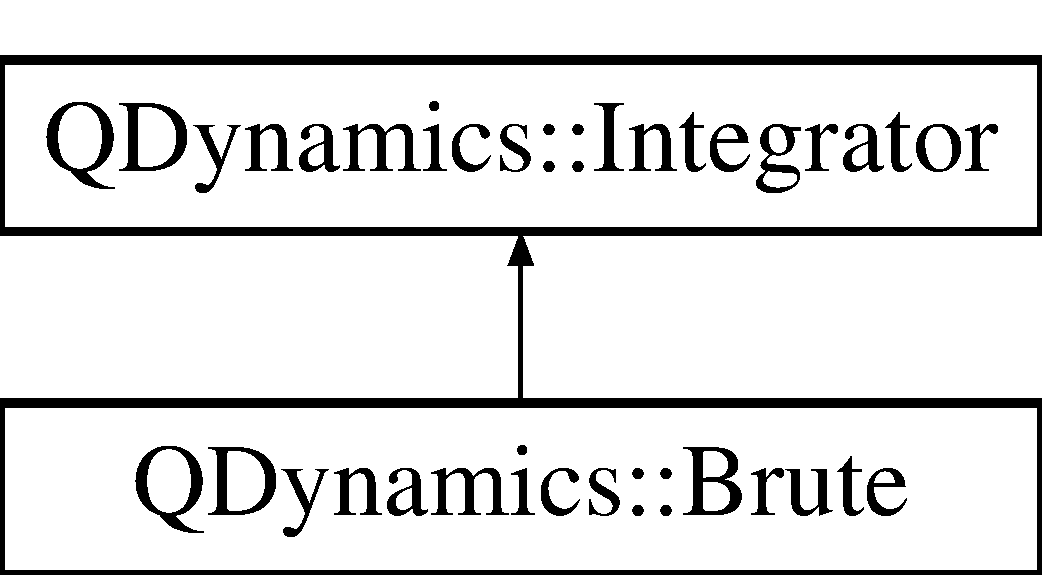
\includegraphics[height=2.000000cm]{classQDynamics_1_1Brute}
\end{center}
\end{figure}
\subsection*{Public Member Functions}
\begin{DoxyCompactItemize}
\item 
\hyperlink{classQDynamics_1_1Brute_a2ef1df08140810ffbc9a3e8b97561bbb}{Brute} (double T, double deltaT)
\item 
\hyperlink{classQDynamics_1_1Brute_a5f04abe903e88405c24fb5695db6357f}{Brute} (double T, double deltaT, int skipper)
\end{DoxyCompactItemize}
\subsection*{Private Member Functions}
\begin{DoxyCompactItemize}
\item 
virtual void \hyperlink{classQDynamics_1_1Brute_ac5d4bbe0e34a9f6836f71f40ae8a9eb4}{Update\+Position} (double t)
\end{DoxyCompactItemize}
\subsection*{Additional Inherited Members}


\subsection{Constructor \& Destructor Documentation}
\mbox{\Hypertarget{classQDynamics_1_1Brute_a2ef1df08140810ffbc9a3e8b97561bbb}\label{classQDynamics_1_1Brute_a2ef1df08140810ffbc9a3e8b97561bbb}} 
\index{Q\+Dynamics\+::\+Brute@{Q\+Dynamics\+::\+Brute}!Brute@{Brute}}
\index{Brute@{Brute}!Q\+Dynamics\+::\+Brute@{Q\+Dynamics\+::\+Brute}}
\subsubsection{\texorpdfstring{Brute()}{Brute()}\hspace{0.1cm}{\footnotesize\ttfamily [1/2]}}
{\footnotesize\ttfamily Q\+Dynamics\+::\+Brute\+::\+Brute (\begin{DoxyParamCaption}\item[{double}]{T,  }\item[{double}]{deltaT }\end{DoxyParamCaption})\hspace{0.3cm}{\ttfamily [inline]}}

\mbox{\Hypertarget{classQDynamics_1_1Brute_a5f04abe903e88405c24fb5695db6357f}\label{classQDynamics_1_1Brute_a5f04abe903e88405c24fb5695db6357f}} 
\index{Q\+Dynamics\+::\+Brute@{Q\+Dynamics\+::\+Brute}!Brute@{Brute}}
\index{Brute@{Brute}!Q\+Dynamics\+::\+Brute@{Q\+Dynamics\+::\+Brute}}
\subsubsection{\texorpdfstring{Brute()}{Brute()}\hspace{0.1cm}{\footnotesize\ttfamily [2/2]}}
{\footnotesize\ttfamily Q\+Dynamics\+::\+Brute\+::\+Brute (\begin{DoxyParamCaption}\item[{double}]{T,  }\item[{double}]{deltaT,  }\item[{int}]{skipper }\end{DoxyParamCaption})\hspace{0.3cm}{\ttfamily [inline]}}



\subsection{Member Function Documentation}
\mbox{\Hypertarget{classQDynamics_1_1Brute_ac5d4bbe0e34a9f6836f71f40ae8a9eb4}\label{classQDynamics_1_1Brute_ac5d4bbe0e34a9f6836f71f40ae8a9eb4}} 
\index{Q\+Dynamics\+::\+Brute@{Q\+Dynamics\+::\+Brute}!Update\+Position@{Update\+Position}}
\index{Update\+Position@{Update\+Position}!Q\+Dynamics\+::\+Brute@{Q\+Dynamics\+::\+Brute}}
\subsubsection{\texorpdfstring{Update\+Position()}{UpdatePosition()}}
{\footnotesize\ttfamily virtual void Q\+Dynamics\+::\+Brute\+::\+Update\+Position (\begin{DoxyParamCaption}\item[{double}]{t }\end{DoxyParamCaption})\hspace{0.3cm}{\ttfamily [inline]}, {\ttfamily [private]}, {\ttfamily [virtual]}}



Reimplemented from \hyperlink{classQDynamics_1_1Integrator_a4effa27d56f3205e53653b1fdc5cd08e}{Q\+Dynamics\+::\+Integrator}.



The documentation for this class was generated from the following file\+:\begin{DoxyCompactItemize}
\item 
/home/f/fraserj/\+Documents/\+Work/\+Q\+Dynamics/src/\hyperlink{Brute_8h}{Brute.\+h}\end{DoxyCompactItemize}

\hypertarget{classQDynamics_1_1Integrator}{}\doxysection{Q\+Dynamics\+::Integrator Class Reference}
\label{classQDynamics_1_1Integrator}\index{QDynamics::Integrator@{QDynamics::Integrator}}


{\ttfamily \#include $<$Integrator.\+h$>$}

Inheritance diagram for Q\+Dynamics\+::Integrator\+:\begin{figure}[H]
\begin{center}
\leavevmode
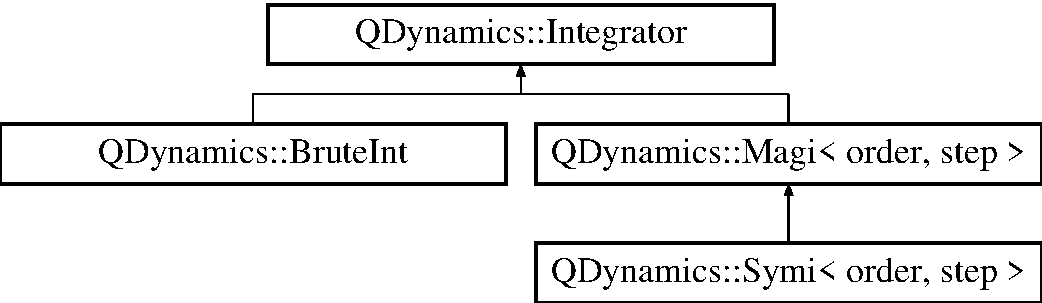
\includegraphics[height=3.000000cm]{classQDynamics_1_1Integrator}
\end{center}
\end{figure}
\doxysubsection*{Public Member Functions}
\begin{DoxyCompactItemize}
\item 
\mbox{\hyperlink{classQDynamics_1_1Integrator_a677dd555cee316d6d456b7da258c4385}{Integrator}} (double T, double deltaT)
\begin{DoxyCompactList}\small\item\em Constructor function. \end{DoxyCompactList}\item 
\mbox{\hyperlink{classQDynamics_1_1Integrator_aa469124cb408fadbaa540555dfabee33}{Integrator}} (double T, double deltaT, int skipper)
\begin{DoxyCompactList}\small\item\em Constructor function. \end{DoxyCompactList}\item 
void \mbox{\hyperlink{classQDynamics_1_1Integrator_a4b921b312775194b77c2c85f93add84e}{Evolve}} (\mbox{\hyperlink{classQDynamics_1_1Quaternion}{Quaternion}} q0, \mbox{\hyperlink{classQDynamics_1_1Quaternion}{Quaternion}} p0, \mbox{\hyperlink{classJSL_1_1Vector}{J\+S\+L\+::\+Vector}} \mbox{\hyperlink{classQDynamics_1_1Integrator_a7b99b22475321b34c1624bded3489954}{J}}, std\+::string save\+Folder)
\item 
virtual void \mbox{\hyperlink{classQDynamics_1_1Integrator_a4effa27d56f3205e53653b1fdc5cd08e}{Update\+Position}} (double t)
\begin{DoxyCompactList}\small\item\em In the \mbox{\hyperlink{classQDynamics_1_1Integrator}{Integrator}} base class, this is an empty function. Child members will mainly focus on overloading this function to their own update formula. \end{DoxyCompactList}\end{DoxyCompactItemize}
\doxysubsection*{Protected Member Functions}
\begin{DoxyCompactItemize}
\item 
virtual \mbox{\hyperlink{classQDynamics_1_1Quaternion}{Quaternion}} \mbox{\hyperlink{classQDynamics_1_1Integrator_a4688fbccd8b0dc5c9a73dddac66b486f}{GradU}} (double t)
\begin{DoxyCompactList}\small\item\em Returns the quaternionic derivative of the neo-\/potential V (equal to the derivative of the rotation potential U), given the current value of \mbox{\hyperlink{classQDynamics_1_1Integrator_a5929511da076c7f31749a6da713fcff6}{Integrator\+::q}} and the current time. \end{DoxyCompactList}\item 
virtual double \mbox{\hyperlink{classQDynamics_1_1Integrator_afa838ba8dfb0fbde1f77c6d2a45a9dd0}{U}} (double t)
\begin{DoxyCompactList}\small\item\em Returns the current value of the rotation potential U, given the current value of \mbox{\hyperlink{classQDynamics_1_1Integrator_a5929511da076c7f31749a6da713fcff6}{Integrator\+::q}} and the current time. Unlike \mbox{\hyperlink{classQDynamics_1_1Integrator_a4688fbccd8b0dc5c9a73dddac66b486f}{Grad\+U()}}, it is not critical that this function be 100\% correct, as it is only used by the \mbox{\hyperlink{classQDynamics_1_1Integrator_a816743f6efb41b0b29243ff3bdaa4c9d}{Integrator\+::\+Hamiltonian}} function as bookkeeping for the current energy. If you do not wish to track the current energy, you may neglect this function. \end{DoxyCompactList}\end{DoxyCompactItemize}
\doxysubsection*{Protected Attributes}
\begin{DoxyCompactItemize}
\item 
\mbox{\hyperlink{classQDynamics_1_1Quaternion}{Quaternion}} \mbox{\hyperlink{classQDynamics_1_1Integrator_a5929511da076c7f31749a6da713fcff6}{q}}
\begin{DoxyCompactList}\small\item\em The current position variable. \end{DoxyCompactList}\item 
\mbox{\hyperlink{classQDynamics_1_1Quaternion}{Quaternion}} \mbox{\hyperlink{classQDynamics_1_1Integrator_a1fb07254408f6ad620eb9dbfa0f8da95}{p}}
\begin{DoxyCompactList}\small\item\em The current momentum variable. \end{DoxyCompactList}\item 
\mbox{\hyperlink{classQDynamics_1_1Quaternion}{Quaternion}} \mbox{\hyperlink{classQDynamics_1_1Integrator_a0241b2e2c87418323330999d1f8e12d0}{w}}
\begin{DoxyCompactList}\small\item\em The current body-\/fixed angular speed. \end{DoxyCompactList}\item 
\mbox{\hyperlink{classQDynamics_1_1Quaternion}{Quaternion}} \mbox{\hyperlink{classQDynamics_1_1Integrator_adb45dae4f4d1d37ab83ca5269f51058d}{L}}
\begin{DoxyCompactList}\small\item\em The current body-\/fixed Angular momentum. \end{DoxyCompactList}\item 
\mbox{\hyperlink{classJSL_1_1Vector}{J\+S\+L\+::\+Vector}} \mbox{\hyperlink{classQDynamics_1_1Integrator_a7b99b22475321b34c1624bded3489954}{J}}
\begin{DoxyCompactList}\small\item\em The saved location of the moment of inertia matrix (see \mbox{\hyperlink{classQDynamics_1_1Integrator_a4b921b312775194b77c2c85f93add84e}{Evolve()}}) \end{DoxyCompactList}\item 
double \mbox{\hyperlink{classQDynamics_1_1Integrator_a9b850dd4b29118e44b0183409db0a983}{Time\+Step}}
\begin{DoxyCompactList}\small\item\em The timestep taken by the integrator. \end{DoxyCompactList}\item 
double \mbox{\hyperlink{classQDynamics_1_1Integrator_addfb67b6faa62d88bc7234d5496aeaf9}{Total\+Time}}
\begin{DoxyCompactList}\small\item\em The total length of time that the integrator will search for. \end{DoxyCompactList}\item 
std\+::string \mbox{\hyperlink{classQDynamics_1_1Integrator_aa3e27d68428619ab4083b2d42ef8924c}{Name}}
\begin{DoxyCompactList}\small\item\em The assigned name of the integrator. This is set to \char`\"{}\+Unassigned\char`\"{} by default\+: child classes should modify this name. \end{DoxyCompactList}\item 
std\+::string \mbox{\hyperlink{classQDynamics_1_1Integrator_a19ed0b9864ebe762914cee04cb0ad4b3}{File\+Name}}
\begin{DoxyCompactList}\small\item\em The location written to by \mbox{\hyperlink{classQDynamics_1_1Integrator_ae80ab509b96a9b996934d9ef127f5137}{Create\+Full\+Name()}}. A file location which will be used to write the output buffer to. \end{DoxyCompactList}\end{DoxyCompactItemize}
\doxysubsection*{Private Member Functions}
\begin{DoxyCompactItemize}
\item 
void \mbox{\hyperlink{classQDynamics_1_1Integrator_af613a42e489de2d041673fd5be0ebb61}{Update\+Buffer}} (double t)
\begin{DoxyCompactList}\small\item\em Called during every loop of \mbox{\hyperlink{classQDynamics_1_1Integrator_a4b921b312775194b77c2c85f93add84e}{Evolve()}}, saves some values of interest to the \mbox{\hyperlink{classQDynamics_1_1Integrator_af8889c2bbe10237a8dd8c46b25b15d29}{Integrator\+::\+Buffer}}. \end{DoxyCompactList}\item 
void \mbox{\hyperlink{classQDynamics_1_1Integrator_a571bd4098f5d245bf46cf7683dcc554a}{Flush\+Buffer}} ()
\begin{DoxyCompactList}\small\item\em Called when the \mbox{\hyperlink{classQDynamics_1_1Integrator_af8889c2bbe10237a8dd8c46b25b15d29}{Integrator\+::\+Buffer}} is full, writes the contents of the buffer to the file determined by \mbox{\hyperlink{classQDynamics_1_1Integrator_a19ed0b9864ebe762914cee04cb0ad4b3}{Integrator\+::\+File\+Name}}, and resets the buffer. \end{DoxyCompactList}\item 
void \mbox{\hyperlink{classQDynamics_1_1Integrator_a88dc286b39899bdec60c040427d663cc}{Update\+Progress\+Bar}} (double t)
\begin{DoxyCompactList}\small\item\em Writes a series of \# to the screen to act as a progress bar\+: \mbox{[}\#\#\#\#\# \mbox{]}. \end{DoxyCompactList}\item 
void \mbox{\hyperlink{classQDynamics_1_1Integrator_aa1afd442ef37708fcadb45ca8e7958f5}{Initialise}} (\mbox{\hyperlink{classQDynamics_1_1Quaternion}{Quaternion}} q0, \mbox{\hyperlink{classQDynamics_1_1Quaternion}{Quaternion}} p0, \mbox{\hyperlink{classJSL_1_1Vector}{J\+S\+L\+::\+Vector}} Jin, std\+::string save\+Folder)
\item 
void \mbox{\hyperlink{classQDynamics_1_1Integrator_ae80ab509b96a9b996934d9ef127f5137}{Create\+Full\+Name}} (std\+::string save\+Folder)
\begin{DoxyCompactList}\small\item\em Computes the \mbox{\hyperlink{classQDynamics_1_1Integrator_a19ed0b9864ebe762914cee04cb0ad4b3}{Integrator\+::\+File\+Name}} including the filepath from from the \mbox{\hyperlink{classQDynamics_1_1Integrator_aa3e27d68428619ab4083b2d42ef8924c}{Integrator\+::\+Name}} and the provided directory. \end{DoxyCompactList}\item 
double \mbox{\hyperlink{classQDynamics_1_1Integrator_a816743f6efb41b0b29243ff3bdaa4c9d}{Hamiltonian}} (double t)
\begin{DoxyCompactList}\small\item\em Computes the current value of the energy of the system given the kinetic energy and the value of \mbox{\hyperlink{classQDynamics_1_1Integrator_afa838ba8dfb0fbde1f77c6d2a45a9dd0}{U()}}. \end{DoxyCompactList}\end{DoxyCompactItemize}
\doxysubsection*{Private Attributes}
\begin{DoxyCompactItemize}
\item 
int \mbox{\hyperlink{classQDynamics_1_1Integrator_ae62176188110c0dcea7c65ba429d1abe}{Buffer\+Pos}}
\begin{DoxyCompactList}\small\item\em The current write-\/index of \mbox{\hyperlink{classQDynamics_1_1Integrator_af8889c2bbe10237a8dd8c46b25b15d29}{Integrator\+::\+Buffer}}. \end{DoxyCompactList}\item 
int \mbox{\hyperlink{classQDynamics_1_1Integrator_acbafc2a1b2b19f230c6dfd8924cb36dd}{Buffer\+Size}}
\begin{DoxyCompactList}\small\item\em The length of the \mbox{\hyperlink{classQDynamics_1_1Integrator_af8889c2bbe10237a8dd8c46b25b15d29}{Integrator\+::\+Buffer}}. \end{DoxyCompactList}\item 
int \mbox{\hyperlink{classQDynamics_1_1Integrator_a00be60876ae62ef0d1555a6cc0ce52a5}{N\+Hashes}}
\begin{DoxyCompactList}\small\item\em The number of hashes a full progress bar is made up of. \end{DoxyCompactList}\item 
bool \mbox{\hyperlink{classQDynamics_1_1Integrator_ae893dd6b0d041de777e25a99f42886c3}{Final\+Hash}}
\begin{DoxyCompactList}\small\item\em A simple lock tracking if the final hash has been written, preventing multiple termination characters being printed. \end{DoxyCompactList}\item 
int \mbox{\hyperlink{classQDynamics_1_1Integrator_abab707f49ba0ae6701db5dbcdf86861f}{Current\+Hashes}}
\begin{DoxyCompactList}\small\item\em The current number of progress hashes which have been written to the terminal. \end{DoxyCompactList}\item 
std\+::vector$<$ std\+::string $>$ \mbox{\hyperlink{classQDynamics_1_1Integrator_af8889c2bbe10237a8dd8c46b25b15d29}{Buffer}}
\begin{DoxyCompactList}\small\item\em A string-\/buffer containing the save-\/values of several past values of the integrator. Once full, the buffer is written to file. \end{DoxyCompactList}\item 
int \mbox{\hyperlink{classQDynamics_1_1Integrator_a95e110d6b14003db39f8a52180b97870}{Skip\+ID}}
\begin{DoxyCompactList}\small\item\em The current number of files that the buffer has skipped (as per the skipper variable in \mbox{\hyperlink{classQDynamics_1_1Integrator_aa469124cb408fadbaa540555dfabee33}{Integrator(double,double,int)}}) \end{DoxyCompactList}\item 
int \mbox{\hyperlink{classQDynamics_1_1Integrator_a409e18faeeefa5fb63f7bcce3eb0e381}{Skips}}
\begin{DoxyCompactList}\small\item\em The maximum value of Skip\+ID before the buffer saves a value. \end{DoxyCompactList}\end{DoxyCompactItemize}


\doxysubsection{Detailed Description}
A superclass from which all individual integrators will inherit. Handles the mundane stuff such as the progress tracking and saving. Importantly, it provides virtual overload methods for Gradu() and \mbox{\hyperlink{classQDynamics_1_1Integrator_afa838ba8dfb0fbde1f77c6d2a45a9dd0}{U()}} which allows external definition of the dynamics, and of \mbox{\hyperlink{classQDynamics_1_1Integrator_a4effa27d56f3205e53653b1fdc5cd08e}{Update\+Position()}} which allows specific subclasses of this object choose how they want to move from q\+\_\+i -\/$>$ q\+\_\+i+1. 

\doxysubsection{Constructor \& Destructor Documentation}
\mbox{\Hypertarget{classQDynamics_1_1Integrator_a677dd555cee316d6d456b7da258c4385}\label{classQDynamics_1_1Integrator_a677dd555cee316d6d456b7da258c4385}} 
\index{QDynamics::Integrator@{QDynamics::Integrator}!Integrator@{Integrator}}
\index{Integrator@{Integrator}!QDynamics::Integrator@{QDynamics::Integrator}}
\doxysubsubsection{\texorpdfstring{Integrator()}{Integrator()}\hspace{0.1cm}{\footnotesize\ttfamily [1/2]}}
{\footnotesize\ttfamily Q\+Dynamics\+::\+Integrator\+::\+Integrator (\begin{DoxyParamCaption}\item[{double}]{T,  }\item[{double}]{deltaT }\end{DoxyParamCaption})\hspace{0.3cm}{\ttfamily [inline]}}



Constructor function. 


\begin{DoxyParams}{Parameters}
{\em T} & The total duration of the integration\\
\hline
{\em deltaT} & the width of timesteps used \\
\hline
\end{DoxyParams}
\mbox{\Hypertarget{classQDynamics_1_1Integrator_aa469124cb408fadbaa540555dfabee33}\label{classQDynamics_1_1Integrator_aa469124cb408fadbaa540555dfabee33}} 
\index{QDynamics::Integrator@{QDynamics::Integrator}!Integrator@{Integrator}}
\index{Integrator@{Integrator}!QDynamics::Integrator@{QDynamics::Integrator}}
\doxysubsubsection{\texorpdfstring{Integrator()}{Integrator()}\hspace{0.1cm}{\footnotesize\ttfamily [2/2]}}
{\footnotesize\ttfamily Q\+Dynamics\+::\+Integrator\+::\+Integrator (\begin{DoxyParamCaption}\item[{double}]{T,  }\item[{double}]{deltaT,  }\item[{int}]{skipper }\end{DoxyParamCaption})\hspace{0.3cm}{\ttfamily [inline]}}



Constructor function. 


\begin{DoxyParams}{Parameters}
{\em T} & The total duration of the integration\\
\hline
{\em deltaT} & the width of timesteps used\\
\hline
{\em skipper} & The number of epochs which pass in between updates to the progess \mbox{\hyperlink{classQDynamics_1_1Integrator_af8889c2bbe10237a8dd8c46b25b15d29}{Integrator\+::\+Buffer}} \\
\hline
\end{DoxyParams}


\doxysubsection{Member Function Documentation}
\mbox{\Hypertarget{classQDynamics_1_1Integrator_ae80ab509b96a9b996934d9ef127f5137}\label{classQDynamics_1_1Integrator_ae80ab509b96a9b996934d9ef127f5137}} 
\index{QDynamics::Integrator@{QDynamics::Integrator}!CreateFullName@{CreateFullName}}
\index{CreateFullName@{CreateFullName}!QDynamics::Integrator@{QDynamics::Integrator}}
\doxysubsubsection{\texorpdfstring{CreateFullName()}{CreateFullName()}}
{\footnotesize\ttfamily void Q\+Dynamics\+::\+Integrator\+::\+Create\+Full\+Name (\begin{DoxyParamCaption}\item[{std\+::string}]{save\+Folder }\end{DoxyParamCaption})\hspace{0.3cm}{\ttfamily [inline]}, {\ttfamily [private]}}



Computes the \mbox{\hyperlink{classQDynamics_1_1Integrator_a19ed0b9864ebe762914cee04cb0ad4b3}{Integrator\+::\+File\+Name}} including the filepath from from the \mbox{\hyperlink{classQDynamics_1_1Integrator_aa3e27d68428619ab4083b2d42ef8924c}{Integrator\+::\+Name}} and the provided directory. 


\begin{DoxyParams}{Parameters}
{\em save\+Folder} & The corresponding value passed to Intitialise() \\
\hline
\end{DoxyParams}
\mbox{\Hypertarget{classQDynamics_1_1Integrator_a4b921b312775194b77c2c85f93add84e}\label{classQDynamics_1_1Integrator_a4b921b312775194b77c2c85f93add84e}} 
\index{QDynamics::Integrator@{QDynamics::Integrator}!Evolve@{Evolve}}
\index{Evolve@{Evolve}!QDynamics::Integrator@{QDynamics::Integrator}}
\doxysubsubsection{\texorpdfstring{Evolve()}{Evolve()}}
{\footnotesize\ttfamily void Q\+Dynamics\+::\+Integrator\+::\+Evolve (\begin{DoxyParamCaption}\item[{\mbox{\hyperlink{classQDynamics_1_1Quaternion}{Quaternion}}}]{q0,  }\item[{\mbox{\hyperlink{classQDynamics_1_1Quaternion}{Quaternion}}}]{p0,  }\item[{\mbox{\hyperlink{classJSL_1_1Vector}{J\+S\+L\+::\+Vector}}}]{J,  }\item[{std\+::string}]{save\+Folder }\end{DoxyParamCaption})\hspace{0.3cm}{\ttfamily [inline]}}

The main computation loop. Calls \mbox{\hyperlink{classQDynamics_1_1Integrator_a4effa27d56f3205e53653b1fdc5cd08e}{Update\+Position()}} at each timestep until the Total\+Time is reached. 
\begin{DoxyParams}{Parameters}
{\em q0} & The initial position \mbox{\hyperlink{classQDynamics_1_1Quaternion}{Quaternion}} \\
\hline
{\em p0} & The initial momentum \mbox{\hyperlink{classQDynamics_1_1Quaternion}{Quaternion}} \\
\hline
{\em J} & The diagonals of the moment of inertia vector (we have implicitly assumed the system triaxial is such that J is diagonal) \\
\hline
{\em save\+Folder} & The location into which the \mbox{\hyperlink{classQDynamics_1_1Integrator_af8889c2bbe10237a8dd8c46b25b15d29}{Integrator\+::\+Buffer}} output is saved. \\
\hline
\end{DoxyParams}
\mbox{\Hypertarget{classQDynamics_1_1Integrator_a571bd4098f5d245bf46cf7683dcc554a}\label{classQDynamics_1_1Integrator_a571bd4098f5d245bf46cf7683dcc554a}} 
\index{QDynamics::Integrator@{QDynamics::Integrator}!FlushBuffer@{FlushBuffer}}
\index{FlushBuffer@{FlushBuffer}!QDynamics::Integrator@{QDynamics::Integrator}}
\doxysubsubsection{\texorpdfstring{FlushBuffer()}{FlushBuffer()}}
{\footnotesize\ttfamily void Q\+Dynamics\+::\+Integrator\+::\+Flush\+Buffer (\begin{DoxyParamCaption}{ }\end{DoxyParamCaption})\hspace{0.3cm}{\ttfamily [inline]}, {\ttfamily [private]}}



Called when the \mbox{\hyperlink{classQDynamics_1_1Integrator_af8889c2bbe10237a8dd8c46b25b15d29}{Integrator\+::\+Buffer}} is full, writes the contents of the buffer to the file determined by \mbox{\hyperlink{classQDynamics_1_1Integrator_a19ed0b9864ebe762914cee04cb0ad4b3}{Integrator\+::\+File\+Name}}, and resets the buffer. 

\mbox{\Hypertarget{classQDynamics_1_1Integrator_a4688fbccd8b0dc5c9a73dddac66b486f}\label{classQDynamics_1_1Integrator_a4688fbccd8b0dc5c9a73dddac66b486f}} 
\index{QDynamics::Integrator@{QDynamics::Integrator}!GradU@{GradU}}
\index{GradU@{GradU}!QDynamics::Integrator@{QDynamics::Integrator}}
\doxysubsubsection{\texorpdfstring{GradU()}{GradU()}}
{\footnotesize\ttfamily virtual \mbox{\hyperlink{classQDynamics_1_1Quaternion}{Quaternion}} Q\+Dynamics\+::\+Integrator\+::\+GradU (\begin{DoxyParamCaption}\item[{double}]{t }\end{DoxyParamCaption})\hspace{0.3cm}{\ttfamily [protected]}, {\ttfamily [virtual]}}



Returns the quaternionic derivative of the neo-\/potential V (equal to the derivative of the rotation potential U), given the current value of \mbox{\hyperlink{classQDynamics_1_1Integrator_a5929511da076c7f31749a6da713fcff6}{Integrator\+::q}} and the current time. 


\begin{DoxyParams}{Parameters}
{\em t} & The current time \\
\hline
\end{DoxyParams}
\begin{DoxyReturn}{Returns}
The value of the quaternionic gradient 
\end{DoxyReturn}
\mbox{\Hypertarget{classQDynamics_1_1Integrator_a816743f6efb41b0b29243ff3bdaa4c9d}\label{classQDynamics_1_1Integrator_a816743f6efb41b0b29243ff3bdaa4c9d}} 
\index{QDynamics::Integrator@{QDynamics::Integrator}!Hamiltonian@{Hamiltonian}}
\index{Hamiltonian@{Hamiltonian}!QDynamics::Integrator@{QDynamics::Integrator}}
\doxysubsubsection{\texorpdfstring{Hamiltonian()}{Hamiltonian()}}
{\footnotesize\ttfamily double Q\+Dynamics\+::\+Integrator\+::\+Hamiltonian (\begin{DoxyParamCaption}\item[{double}]{t }\end{DoxyParamCaption})\hspace{0.3cm}{\ttfamily [inline]}, {\ttfamily [private]}}



Computes the current value of the energy of the system given the kinetic energy and the value of \mbox{\hyperlink{classQDynamics_1_1Integrator_afa838ba8dfb0fbde1f77c6d2a45a9dd0}{U()}}. 


\begin{DoxyParams}{Parameters}
{\em t} & The current time, for time-\/dependent potentials. \\
\hline
\end{DoxyParams}
\mbox{\Hypertarget{classQDynamics_1_1Integrator_aa1afd442ef37708fcadb45ca8e7958f5}\label{classQDynamics_1_1Integrator_aa1afd442ef37708fcadb45ca8e7958f5}} 
\index{QDynamics::Integrator@{QDynamics::Integrator}!Initialise@{Initialise}}
\index{Initialise@{Initialise}!QDynamics::Integrator@{QDynamics::Integrator}}
\doxysubsubsection{\texorpdfstring{Initialise()}{Initialise()}}
{\footnotesize\ttfamily void Q\+Dynamics\+::\+Integrator\+::\+Initialise (\begin{DoxyParamCaption}\item[{\mbox{\hyperlink{classQDynamics_1_1Quaternion}{Quaternion}}}]{q0,  }\item[{\mbox{\hyperlink{classQDynamics_1_1Quaternion}{Quaternion}}}]{p0,  }\item[{\mbox{\hyperlink{classJSL_1_1Vector}{J\+S\+L\+::\+Vector}}}]{Jin,  }\item[{std\+::string}]{save\+Folder }\end{DoxyParamCaption})\hspace{0.3cm}{\ttfamily [inline]}, {\ttfamily [private]}}

Prepares the \mbox{\hyperlink{classQDynamics_1_1Integrator}{Integrator}} for a new computation loop. Called at the start of an \mbox{\hyperlink{classQDynamics_1_1Integrator_a4b921b312775194b77c2c85f93add84e}{Evolve()}} process, it wipes the buffer and prepares the output file. The inputs are simply those passed to \mbox{\hyperlink{classQDynamics_1_1Integrator_a4b921b312775194b77c2c85f93add84e}{Evolve()}} 
\begin{DoxyParams}{Parameters}
{\em q0} & The initial position \mbox{\hyperlink{classQDynamics_1_1Quaternion}{Quaternion}} \\
\hline
{\em p0} & The initial momentum \mbox{\hyperlink{classQDynamics_1_1Quaternion}{Quaternion}} \\
\hline
{\em Jin} & The diagonals of the moment of inertia vector (we have implicitly assumed the system triaxial is such that J is diagonal) \\
\hline
{\em save\+Folder} & The location into which the \mbox{\hyperlink{classQDynamics_1_1Integrator_af8889c2bbe10237a8dd8c46b25b15d29}{Integrator\+::\+Buffer}} output is saved. \\
\hline
\end{DoxyParams}
\mbox{\Hypertarget{classQDynamics_1_1Integrator_afa838ba8dfb0fbde1f77c6d2a45a9dd0}\label{classQDynamics_1_1Integrator_afa838ba8dfb0fbde1f77c6d2a45a9dd0}} 
\index{QDynamics::Integrator@{QDynamics::Integrator}!U@{U}}
\index{U@{U}!QDynamics::Integrator@{QDynamics::Integrator}}
\doxysubsubsection{\texorpdfstring{U()}{U()}}
{\footnotesize\ttfamily virtual double Q\+Dynamics\+::\+Integrator\+::U (\begin{DoxyParamCaption}\item[{double}]{t }\end{DoxyParamCaption})\hspace{0.3cm}{\ttfamily [protected]}, {\ttfamily [virtual]}}



Returns the current value of the rotation potential U, given the current value of \mbox{\hyperlink{classQDynamics_1_1Integrator_a5929511da076c7f31749a6da713fcff6}{Integrator\+::q}} and the current time. Unlike \mbox{\hyperlink{classQDynamics_1_1Integrator_a4688fbccd8b0dc5c9a73dddac66b486f}{Grad\+U()}}, it is not critical that this function be 100\% correct, as it is only used by the \mbox{\hyperlink{classQDynamics_1_1Integrator_a816743f6efb41b0b29243ff3bdaa4c9d}{Integrator\+::\+Hamiltonian}} function as bookkeeping for the current energy. If you do not wish to track the current energy, you may neglect this function. 


\begin{DoxyParams}{Parameters}
{\em t} & The current time \\
\hline
\end{DoxyParams}
\begin{DoxyReturn}{Returns}
The current potential energy of the system 
\end{DoxyReturn}
\mbox{\Hypertarget{classQDynamics_1_1Integrator_af613a42e489de2d041673fd5be0ebb61}\label{classQDynamics_1_1Integrator_af613a42e489de2d041673fd5be0ebb61}} 
\index{QDynamics::Integrator@{QDynamics::Integrator}!UpdateBuffer@{UpdateBuffer}}
\index{UpdateBuffer@{UpdateBuffer}!QDynamics::Integrator@{QDynamics::Integrator}}
\doxysubsubsection{\texorpdfstring{UpdateBuffer()}{UpdateBuffer()}}
{\footnotesize\ttfamily void Q\+Dynamics\+::\+Integrator\+::\+Update\+Buffer (\begin{DoxyParamCaption}\item[{double}]{t }\end{DoxyParamCaption})\hspace{0.3cm}{\ttfamily [inline]}, {\ttfamily [private]}}



Called during every loop of \mbox{\hyperlink{classQDynamics_1_1Integrator_a4b921b312775194b77c2c85f93add84e}{Evolve()}}, saves some values of interest to the \mbox{\hyperlink{classQDynamics_1_1Integrator_af8889c2bbe10237a8dd8c46b25b15d29}{Integrator\+::\+Buffer}}. 


\begin{DoxyParams}{Parameters}
{\em t} & The current time, needed as part of the buffer input \\
\hline
\end{DoxyParams}
\mbox{\Hypertarget{classQDynamics_1_1Integrator_a4effa27d56f3205e53653b1fdc5cd08e}\label{classQDynamics_1_1Integrator_a4effa27d56f3205e53653b1fdc5cd08e}} 
\index{QDynamics::Integrator@{QDynamics::Integrator}!UpdatePosition@{UpdatePosition}}
\index{UpdatePosition@{UpdatePosition}!QDynamics::Integrator@{QDynamics::Integrator}}
\doxysubsubsection{\texorpdfstring{UpdatePosition()}{UpdatePosition()}}
{\footnotesize\ttfamily virtual void Q\+Dynamics\+::\+Integrator\+::\+Update\+Position (\begin{DoxyParamCaption}\item[{double}]{t }\end{DoxyParamCaption})\hspace{0.3cm}{\ttfamily [inline]}, {\ttfamily [virtual]}}



In the \mbox{\hyperlink{classQDynamics_1_1Integrator}{Integrator}} base class, this is an empty function. Child members will mainly focus on overloading this function to their own update formula. 


\begin{DoxyParams}{Parameters}
{\em t} & The current time of the integrator \\
\hline
\end{DoxyParams}


Reimplemented in \mbox{\hyperlink{classQDynamics_1_1BruteInt_a0f3d901d692a8f30365d1692c678ce61}{Q\+Dynamics\+::\+Brute\+Int}}, and \mbox{\hyperlink{classQDynamics_1_1Magi_acd1d417b0e03a41ae83422c5b67f77bf}{Q\+Dynamics\+::\+Magi$<$ order, step $>$}}.

\mbox{\Hypertarget{classQDynamics_1_1Integrator_a88dc286b39899bdec60c040427d663cc}\label{classQDynamics_1_1Integrator_a88dc286b39899bdec60c040427d663cc}} 
\index{QDynamics::Integrator@{QDynamics::Integrator}!UpdateProgressBar@{UpdateProgressBar}}
\index{UpdateProgressBar@{UpdateProgressBar}!QDynamics::Integrator@{QDynamics::Integrator}}
\doxysubsubsection{\texorpdfstring{UpdateProgressBar()}{UpdateProgressBar()}}
{\footnotesize\ttfamily void Q\+Dynamics\+::\+Integrator\+::\+Update\+Progress\+Bar (\begin{DoxyParamCaption}\item[{double}]{t }\end{DoxyParamCaption})\hspace{0.3cm}{\ttfamily [inline]}, {\ttfamily [private]}}



Writes a series of \# to the screen to act as a progress bar\+: \mbox{[}\#\#\#\#\# \mbox{]}. 


\begin{DoxyParams}{Parameters}
{\em t} & The current time, so that the current progress can be computed. \\
\hline
\end{DoxyParams}


\doxysubsection{Field Documentation}
\mbox{\Hypertarget{classQDynamics_1_1Integrator_af8889c2bbe10237a8dd8c46b25b15d29}\label{classQDynamics_1_1Integrator_af8889c2bbe10237a8dd8c46b25b15d29}} 
\index{QDynamics::Integrator@{QDynamics::Integrator}!Buffer@{Buffer}}
\index{Buffer@{Buffer}!QDynamics::Integrator@{QDynamics::Integrator}}
\doxysubsubsection{\texorpdfstring{Buffer}{Buffer}}
{\footnotesize\ttfamily std\+::vector$<$std\+::string$>$ Q\+Dynamics\+::\+Integrator\+::\+Buffer\hspace{0.3cm}{\ttfamily [private]}}



A string-\/buffer containing the save-\/values of several past values of the integrator. Once full, the buffer is written to file. 

\mbox{\Hypertarget{classQDynamics_1_1Integrator_ae62176188110c0dcea7c65ba429d1abe}\label{classQDynamics_1_1Integrator_ae62176188110c0dcea7c65ba429d1abe}} 
\index{QDynamics::Integrator@{QDynamics::Integrator}!BufferPos@{BufferPos}}
\index{BufferPos@{BufferPos}!QDynamics::Integrator@{QDynamics::Integrator}}
\doxysubsubsection{\texorpdfstring{BufferPos}{BufferPos}}
{\footnotesize\ttfamily int Q\+Dynamics\+::\+Integrator\+::\+Buffer\+Pos\hspace{0.3cm}{\ttfamily [private]}}



The current write-\/index of \mbox{\hyperlink{classQDynamics_1_1Integrator_af8889c2bbe10237a8dd8c46b25b15d29}{Integrator\+::\+Buffer}}. 

\mbox{\Hypertarget{classQDynamics_1_1Integrator_acbafc2a1b2b19f230c6dfd8924cb36dd}\label{classQDynamics_1_1Integrator_acbafc2a1b2b19f230c6dfd8924cb36dd}} 
\index{QDynamics::Integrator@{QDynamics::Integrator}!BufferSize@{BufferSize}}
\index{BufferSize@{BufferSize}!QDynamics::Integrator@{QDynamics::Integrator}}
\doxysubsubsection{\texorpdfstring{BufferSize}{BufferSize}}
{\footnotesize\ttfamily int Q\+Dynamics\+::\+Integrator\+::\+Buffer\+Size\hspace{0.3cm}{\ttfamily [private]}}



The length of the \mbox{\hyperlink{classQDynamics_1_1Integrator_af8889c2bbe10237a8dd8c46b25b15d29}{Integrator\+::\+Buffer}}. 

\mbox{\Hypertarget{classQDynamics_1_1Integrator_abab707f49ba0ae6701db5dbcdf86861f}\label{classQDynamics_1_1Integrator_abab707f49ba0ae6701db5dbcdf86861f}} 
\index{QDynamics::Integrator@{QDynamics::Integrator}!CurrentHashes@{CurrentHashes}}
\index{CurrentHashes@{CurrentHashes}!QDynamics::Integrator@{QDynamics::Integrator}}
\doxysubsubsection{\texorpdfstring{CurrentHashes}{CurrentHashes}}
{\footnotesize\ttfamily int Q\+Dynamics\+::\+Integrator\+::\+Current\+Hashes\hspace{0.3cm}{\ttfamily [private]}}



The current number of progress hashes which have been written to the terminal. 

\mbox{\Hypertarget{classQDynamics_1_1Integrator_a19ed0b9864ebe762914cee04cb0ad4b3}\label{classQDynamics_1_1Integrator_a19ed0b9864ebe762914cee04cb0ad4b3}} 
\index{QDynamics::Integrator@{QDynamics::Integrator}!FileName@{FileName}}
\index{FileName@{FileName}!QDynamics::Integrator@{QDynamics::Integrator}}
\doxysubsubsection{\texorpdfstring{FileName}{FileName}}
{\footnotesize\ttfamily std\+::string Q\+Dynamics\+::\+Integrator\+::\+File\+Name\hspace{0.3cm}{\ttfamily [protected]}}



The location written to by \mbox{\hyperlink{classQDynamics_1_1Integrator_ae80ab509b96a9b996934d9ef127f5137}{Create\+Full\+Name()}}. A file location which will be used to write the output buffer to. 

\mbox{\Hypertarget{classQDynamics_1_1Integrator_ae893dd6b0d041de777e25a99f42886c3}\label{classQDynamics_1_1Integrator_ae893dd6b0d041de777e25a99f42886c3}} 
\index{QDynamics::Integrator@{QDynamics::Integrator}!FinalHash@{FinalHash}}
\index{FinalHash@{FinalHash}!QDynamics::Integrator@{QDynamics::Integrator}}
\doxysubsubsection{\texorpdfstring{FinalHash}{FinalHash}}
{\footnotesize\ttfamily bool Q\+Dynamics\+::\+Integrator\+::\+Final\+Hash\hspace{0.3cm}{\ttfamily [private]}}



A simple lock tracking if the final hash has been written, preventing multiple termination characters being printed. 

\mbox{\Hypertarget{classQDynamics_1_1Integrator_a7b99b22475321b34c1624bded3489954}\label{classQDynamics_1_1Integrator_a7b99b22475321b34c1624bded3489954}} 
\index{QDynamics::Integrator@{QDynamics::Integrator}!J@{J}}
\index{J@{J}!QDynamics::Integrator@{QDynamics::Integrator}}
\doxysubsubsection{\texorpdfstring{J}{J}}
{\footnotesize\ttfamily \mbox{\hyperlink{classJSL_1_1Vector}{J\+S\+L\+::\+Vector}} Q\+Dynamics\+::\+Integrator\+::J\hspace{0.3cm}{\ttfamily [protected]}}



The saved location of the moment of inertia matrix (see \mbox{\hyperlink{classQDynamics_1_1Integrator_a4b921b312775194b77c2c85f93add84e}{Evolve()}}) 

\mbox{\Hypertarget{classQDynamics_1_1Integrator_adb45dae4f4d1d37ab83ca5269f51058d}\label{classQDynamics_1_1Integrator_adb45dae4f4d1d37ab83ca5269f51058d}} 
\index{QDynamics::Integrator@{QDynamics::Integrator}!L@{L}}
\index{L@{L}!QDynamics::Integrator@{QDynamics::Integrator}}
\doxysubsubsection{\texorpdfstring{L}{L}}
{\footnotesize\ttfamily \mbox{\hyperlink{classQDynamics_1_1Quaternion}{Quaternion}} Q\+Dynamics\+::\+Integrator\+::L\hspace{0.3cm}{\ttfamily [protected]}}



The current body-\/fixed Angular momentum. 

\mbox{\Hypertarget{classQDynamics_1_1Integrator_aa3e27d68428619ab4083b2d42ef8924c}\label{classQDynamics_1_1Integrator_aa3e27d68428619ab4083b2d42ef8924c}} 
\index{QDynamics::Integrator@{QDynamics::Integrator}!Name@{Name}}
\index{Name@{Name}!QDynamics::Integrator@{QDynamics::Integrator}}
\doxysubsubsection{\texorpdfstring{Name}{Name}}
{\footnotesize\ttfamily std\+::string Q\+Dynamics\+::\+Integrator\+::\+Name\hspace{0.3cm}{\ttfamily [protected]}}



The assigned name of the integrator. This is set to \char`\"{}\+Unassigned\char`\"{} by default\+: child classes should modify this name. 

\mbox{\Hypertarget{classQDynamics_1_1Integrator_a00be60876ae62ef0d1555a6cc0ce52a5}\label{classQDynamics_1_1Integrator_a00be60876ae62ef0d1555a6cc0ce52a5}} 
\index{QDynamics::Integrator@{QDynamics::Integrator}!NHashes@{NHashes}}
\index{NHashes@{NHashes}!QDynamics::Integrator@{QDynamics::Integrator}}
\doxysubsubsection{\texorpdfstring{NHashes}{NHashes}}
{\footnotesize\ttfamily int Q\+Dynamics\+::\+Integrator\+::\+N\+Hashes\hspace{0.3cm}{\ttfamily [private]}}



The number of hashes a full progress bar is made up of. 

\mbox{\Hypertarget{classQDynamics_1_1Integrator_a1fb07254408f6ad620eb9dbfa0f8da95}\label{classQDynamics_1_1Integrator_a1fb07254408f6ad620eb9dbfa0f8da95}} 
\index{QDynamics::Integrator@{QDynamics::Integrator}!p@{p}}
\index{p@{p}!QDynamics::Integrator@{QDynamics::Integrator}}
\doxysubsubsection{\texorpdfstring{p}{p}}
{\footnotesize\ttfamily \mbox{\hyperlink{classQDynamics_1_1Quaternion}{Quaternion}} Q\+Dynamics\+::\+Integrator\+::p\hspace{0.3cm}{\ttfamily [protected]}}



The current momentum variable. 

\mbox{\Hypertarget{classQDynamics_1_1Integrator_a5929511da076c7f31749a6da713fcff6}\label{classQDynamics_1_1Integrator_a5929511da076c7f31749a6da713fcff6}} 
\index{QDynamics::Integrator@{QDynamics::Integrator}!q@{q}}
\index{q@{q}!QDynamics::Integrator@{QDynamics::Integrator}}
\doxysubsubsection{\texorpdfstring{q}{q}}
{\footnotesize\ttfamily \mbox{\hyperlink{classQDynamics_1_1Quaternion}{Quaternion}} Q\+Dynamics\+::\+Integrator\+::q\hspace{0.3cm}{\ttfamily [protected]}}



The current position variable. 

\mbox{\Hypertarget{classQDynamics_1_1Integrator_a95e110d6b14003db39f8a52180b97870}\label{classQDynamics_1_1Integrator_a95e110d6b14003db39f8a52180b97870}} 
\index{QDynamics::Integrator@{QDynamics::Integrator}!SkipID@{SkipID}}
\index{SkipID@{SkipID}!QDynamics::Integrator@{QDynamics::Integrator}}
\doxysubsubsection{\texorpdfstring{SkipID}{SkipID}}
{\footnotesize\ttfamily int Q\+Dynamics\+::\+Integrator\+::\+Skip\+ID\hspace{0.3cm}{\ttfamily [private]}}



The current number of files that the buffer has skipped (as per the skipper variable in \mbox{\hyperlink{classQDynamics_1_1Integrator_aa469124cb408fadbaa540555dfabee33}{Integrator(double,double,int)}}) 

\mbox{\Hypertarget{classQDynamics_1_1Integrator_a409e18faeeefa5fb63f7bcce3eb0e381}\label{classQDynamics_1_1Integrator_a409e18faeeefa5fb63f7bcce3eb0e381}} 
\index{QDynamics::Integrator@{QDynamics::Integrator}!Skips@{Skips}}
\index{Skips@{Skips}!QDynamics::Integrator@{QDynamics::Integrator}}
\doxysubsubsection{\texorpdfstring{Skips}{Skips}}
{\footnotesize\ttfamily int Q\+Dynamics\+::\+Integrator\+::\+Skips\hspace{0.3cm}{\ttfamily [private]}}



The maximum value of Skip\+ID before the buffer saves a value. 

\mbox{\Hypertarget{classQDynamics_1_1Integrator_a9b850dd4b29118e44b0183409db0a983}\label{classQDynamics_1_1Integrator_a9b850dd4b29118e44b0183409db0a983}} 
\index{QDynamics::Integrator@{QDynamics::Integrator}!TimeStep@{TimeStep}}
\index{TimeStep@{TimeStep}!QDynamics::Integrator@{QDynamics::Integrator}}
\doxysubsubsection{\texorpdfstring{TimeStep}{TimeStep}}
{\footnotesize\ttfamily double Q\+Dynamics\+::\+Integrator\+::\+Time\+Step\hspace{0.3cm}{\ttfamily [protected]}}



The timestep taken by the integrator. 

\mbox{\Hypertarget{classQDynamics_1_1Integrator_addfb67b6faa62d88bc7234d5496aeaf9}\label{classQDynamics_1_1Integrator_addfb67b6faa62d88bc7234d5496aeaf9}} 
\index{QDynamics::Integrator@{QDynamics::Integrator}!TotalTime@{TotalTime}}
\index{TotalTime@{TotalTime}!QDynamics::Integrator@{QDynamics::Integrator}}
\doxysubsubsection{\texorpdfstring{TotalTime}{TotalTime}}
{\footnotesize\ttfamily double Q\+Dynamics\+::\+Integrator\+::\+Total\+Time\hspace{0.3cm}{\ttfamily [protected]}}



The total length of time that the integrator will search for. 

\mbox{\Hypertarget{classQDynamics_1_1Integrator_a0241b2e2c87418323330999d1f8e12d0}\label{classQDynamics_1_1Integrator_a0241b2e2c87418323330999d1f8e12d0}} 
\index{QDynamics::Integrator@{QDynamics::Integrator}!w@{w}}
\index{w@{w}!QDynamics::Integrator@{QDynamics::Integrator}}
\doxysubsubsection{\texorpdfstring{w}{w}}
{\footnotesize\ttfamily \mbox{\hyperlink{classQDynamics_1_1Quaternion}{Quaternion}} Q\+Dynamics\+::\+Integrator\+::w\hspace{0.3cm}{\ttfamily [protected]}}



The current body-\/fixed angular speed. 



The documentation for this class was generated from the following file\+:\begin{DoxyCompactItemize}
\item 
/home/jack/\+Documents/\+Work/\+Q\+Dynamics/src/\mbox{\hyperlink{Integrator_8h}{Integrator.\+h}}\end{DoxyCompactItemize}

\hypertarget{classJSL__Testing_1_1IOTest}{}\doxysection{J\+S\+L\+\_\+\+Testing\+::I\+O\+Test Class Reference}
\label{classJSL__Testing_1_1IOTest}\index{JSL\_Testing::IOTest@{JSL\_Testing::IOTest}}


{\ttfamily \#include $<$Testing\+\_\+\+Unit\+Tests.\+h$>$}

Inheritance diagram for J\+S\+L\+\_\+\+Testing\+::I\+O\+Test\+:\begin{figure}[H]
\begin{center}
\leavevmode
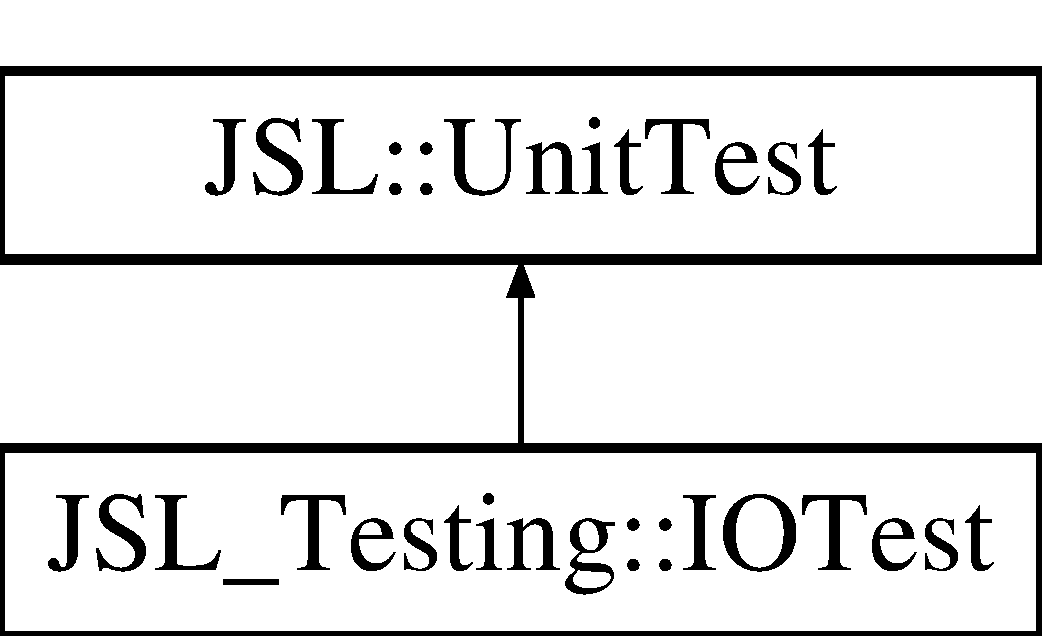
\includegraphics[height=2.000000cm]{classJSL__Testing_1_1IOTest}
\end{center}
\end{figure}
\doxysubsection*{Public Member Functions}
\begin{DoxyCompactItemize}
\item 
\mbox{\hyperlink{classJSL__Testing_1_1IOTest_a75479573809562118ab4d233c2bc0471}{I\+O\+Test}} ()
\item 
void \mbox{\hyperlink{classJSL__Testing_1_1IOTest_a85daecacc71354b5dc0dee36840b8704}{Run\+\_\+\+Test}} ()
\begin{DoxyCompactList}\small\item\em All children which want to take advantage of the \mbox{\hyperlink{classJSL_1_1UnitTest_aabec19b081be8a428f12e4b5e3dc2a9c}{Buffered\+Test()}} command should have the bulk of their testing within this command. \end{DoxyCompactList}\end{DoxyCompactItemize}
\doxysubsection*{Additional Inherited Members}


\doxysubsection{Constructor \& Destructor Documentation}
\mbox{\Hypertarget{classJSL__Testing_1_1IOTest_a75479573809562118ab4d233c2bc0471}\label{classJSL__Testing_1_1IOTest_a75479573809562118ab4d233c2bc0471}} 
\index{JSL\_Testing::IOTest@{JSL\_Testing::IOTest}!IOTest@{IOTest}}
\index{IOTest@{IOTest}!JSL\_Testing::IOTest@{JSL\_Testing::IOTest}}
\doxysubsubsection{\texorpdfstring{IOTest()}{IOTest()}}
{\footnotesize\ttfamily J\+S\+L\+\_\+\+Testing\+::\+I\+O\+Test\+::\+I\+O\+Test (\begin{DoxyParamCaption}{ }\end{DoxyParamCaption})\hspace{0.3cm}{\ttfamily [inline]}}



\doxysubsection{Member Function Documentation}
\mbox{\Hypertarget{classJSL__Testing_1_1IOTest_a85daecacc71354b5dc0dee36840b8704}\label{classJSL__Testing_1_1IOTest_a85daecacc71354b5dc0dee36840b8704}} 
\index{JSL\_Testing::IOTest@{JSL\_Testing::IOTest}!Run\_Test@{Run\_Test}}
\index{Run\_Test@{Run\_Test}!JSL\_Testing::IOTest@{JSL\_Testing::IOTest}}
\doxysubsubsection{\texorpdfstring{Run\_Test()}{Run\_Test()}}
{\footnotesize\ttfamily void J\+S\+L\+\_\+\+Testing\+::\+I\+O\+Test\+::\+Run\+\_\+\+Test (\begin{DoxyParamCaption}{ }\end{DoxyParamCaption})\hspace{0.3cm}{\ttfamily [inline]}, {\ttfamily [virtual]}}



All children which want to take advantage of the \mbox{\hyperlink{classJSL_1_1UnitTest_aabec19b081be8a428f12e4b5e3dc2a9c}{Buffered\+Test()}} command should have the bulk of their testing within this command. 



Reimplemented from \mbox{\hyperlink{classJSL_1_1UnitTest_aa8369ab1ce2a537bff2ea7e1c8818490}{J\+S\+L\+::\+Unit\+Test}}.



The documentation for this class was generated from the following file\+:\begin{DoxyCompactItemize}
\item 
/home/jack/\+Documents/\+Work/\+Q\+Dynamics/lib/\+J\+S\+L/\+Testing/\mbox{\hyperlink{Testing__UnitTests_8h}{Testing\+\_\+\+Unit\+Tests.\+h}}\end{DoxyCompactItemize}

\hypertarget{classQDynamics_1_1Leapi}{}\section{Q\+Dynamics\+:\+:Leapi Class Reference}
\label{classQDynamics_1_1Leapi}\index{Q\+Dynamics\+::\+Leapi@{Q\+Dynamics\+::\+Leapi}}


{\ttfamily \#include $<$Magi.\+h$>$}

Inheritance diagram for Q\+Dynamics\+:\+:Leapi\+:\begin{figure}[H]
\begin{center}
\leavevmode
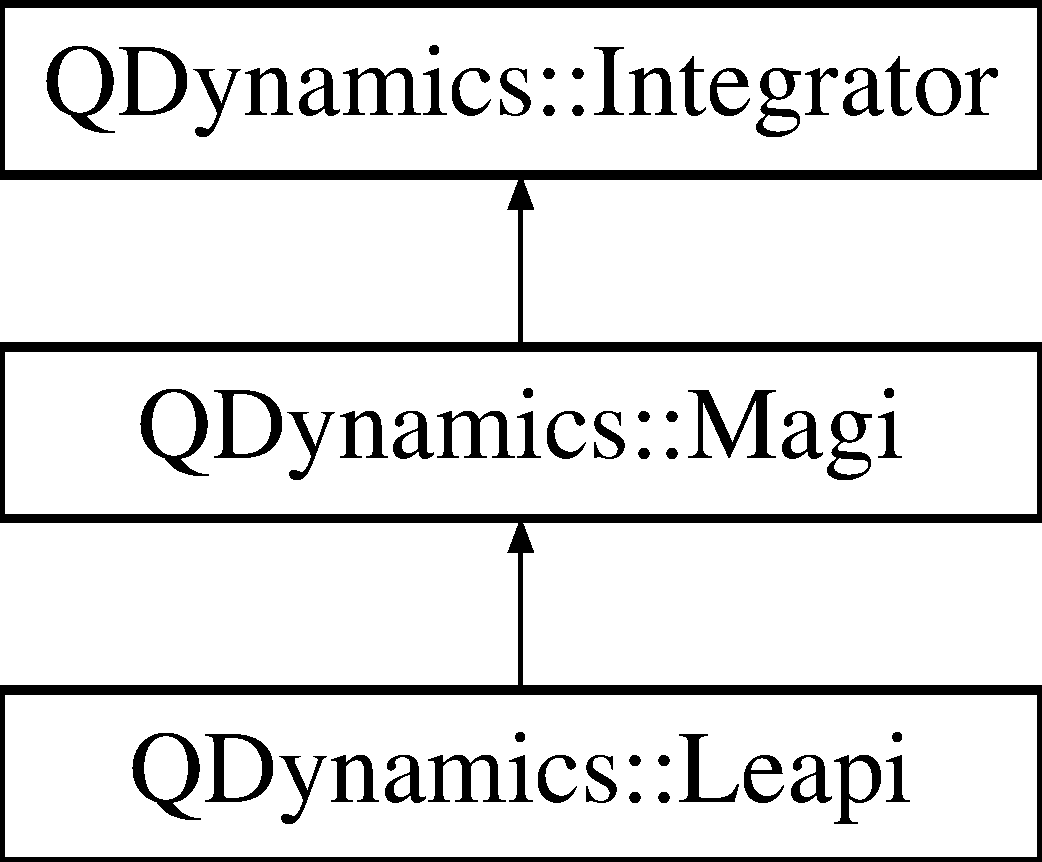
\includegraphics[height=3.000000cm]{classQDynamics_1_1Leapi}
\end{center}
\end{figure}
\subsection*{Public Member Functions}
\begin{DoxyCompactItemize}
\item 
\hyperlink{classQDynamics_1_1Leapi_aa6feac37d39339e26f89626f7bdbc8f0}{Leapi} (int order, int resolution, double T, double deltaT)
\item 
\hyperlink{classQDynamics_1_1Leapi_a008a9a757055debd2e1da2b5ac64a746}{Leapi} (int order, int resolution, double T, double deltaT, int skipper)
\end{DoxyCompactItemize}
\subsection*{Private Member Functions}
\begin{DoxyCompactItemize}
\item 
virtual void \hyperlink{classQDynamics_1_1Leapi_ada2b4935513fa7e0cb4f78ade9f2fd0e}{Update\+Position} (double t)
\begin{DoxyCompactList}\small\item\em In the \hyperlink{classQDynamics_1_1Integrator}{Integrator} base class, this is an empty function. Child members will mainly focus on overloading this function to their own update formula. \end{DoxyCompactList}\end{DoxyCompactItemize}
\subsection*{Additional Inherited Members}


\subsection{Constructor \& Destructor Documentation}
\mbox{\Hypertarget{classQDynamics_1_1Leapi_aa6feac37d39339e26f89626f7bdbc8f0}\label{classQDynamics_1_1Leapi_aa6feac37d39339e26f89626f7bdbc8f0}} 
\index{Q\+Dynamics\+::\+Leapi@{Q\+Dynamics\+::\+Leapi}!Leapi@{Leapi}}
\index{Leapi@{Leapi}!Q\+Dynamics\+::\+Leapi@{Q\+Dynamics\+::\+Leapi}}
\subsubsection{\texorpdfstring{Leapi()}{Leapi()}\hspace{0.1cm}{\footnotesize\ttfamily [1/2]}}
{\footnotesize\ttfamily Q\+Dynamics\+::\+Leapi\+::\+Leapi (\begin{DoxyParamCaption}\item[{int}]{order,  }\item[{int}]{resolution,  }\item[{double}]{T,  }\item[{double}]{deltaT }\end{DoxyParamCaption})\hspace{0.3cm}{\ttfamily [inline]}}

\mbox{\Hypertarget{classQDynamics_1_1Leapi_a008a9a757055debd2e1da2b5ac64a746}\label{classQDynamics_1_1Leapi_a008a9a757055debd2e1da2b5ac64a746}} 
\index{Q\+Dynamics\+::\+Leapi@{Q\+Dynamics\+::\+Leapi}!Leapi@{Leapi}}
\index{Leapi@{Leapi}!Q\+Dynamics\+::\+Leapi@{Q\+Dynamics\+::\+Leapi}}
\subsubsection{\texorpdfstring{Leapi()}{Leapi()}\hspace{0.1cm}{\footnotesize\ttfamily [2/2]}}
{\footnotesize\ttfamily Q\+Dynamics\+::\+Leapi\+::\+Leapi (\begin{DoxyParamCaption}\item[{int}]{order,  }\item[{int}]{resolution,  }\item[{double}]{T,  }\item[{double}]{deltaT,  }\item[{int}]{skipper }\end{DoxyParamCaption})\hspace{0.3cm}{\ttfamily [inline]}}



\subsection{Member Function Documentation}
\mbox{\Hypertarget{classQDynamics_1_1Leapi_ada2b4935513fa7e0cb4f78ade9f2fd0e}\label{classQDynamics_1_1Leapi_ada2b4935513fa7e0cb4f78ade9f2fd0e}} 
\index{Q\+Dynamics\+::\+Leapi@{Q\+Dynamics\+::\+Leapi}!Update\+Position@{Update\+Position}}
\index{Update\+Position@{Update\+Position}!Q\+Dynamics\+::\+Leapi@{Q\+Dynamics\+::\+Leapi}}
\subsubsection{\texorpdfstring{Update\+Position()}{UpdatePosition()}}
{\footnotesize\ttfamily virtual void Q\+Dynamics\+::\+Leapi\+::\+Update\+Position (\begin{DoxyParamCaption}\item[{double}]{t }\end{DoxyParamCaption})\hspace{0.3cm}{\ttfamily [inline]}, {\ttfamily [private]}, {\ttfamily [virtual]}}



In the \hyperlink{classQDynamics_1_1Integrator}{Integrator} base class, this is an empty function. Child members will mainly focus on overloading this function to their own update formula. 


\begin{DoxyParams}{Parameters}
{\em t} & The current time of the integrator \\
\hline
\end{DoxyParams}


Reimplemented from \hyperlink{classQDynamics_1_1Magi_a500467f899244edfae15f34c84c7684c}{Q\+Dynamics\+::\+Magi}.



The documentation for this class was generated from the following file\+:\begin{DoxyCompactItemize}
\item 
/home/f/fraserj/\+Documents/\+Work/\+Q\+Dynamics/src/\hyperlink{Magi_8h}{Magi.\+h}\end{DoxyCompactItemize}

\hypertarget{classQDynamics_1_1Magi}{}\section{Q\+Dynamics\+:\+:Magi Class Reference}
\label{classQDynamics_1_1Magi}\index{Q\+Dynamics\+::\+Magi@{Q\+Dynamics\+::\+Magi}}


{\ttfamily \#include $<$Magi.\+h$>$}

Inheritance diagram for Q\+Dynamics\+:\+:Magi\+:\begin{figure}[H]
\begin{center}
\leavevmode
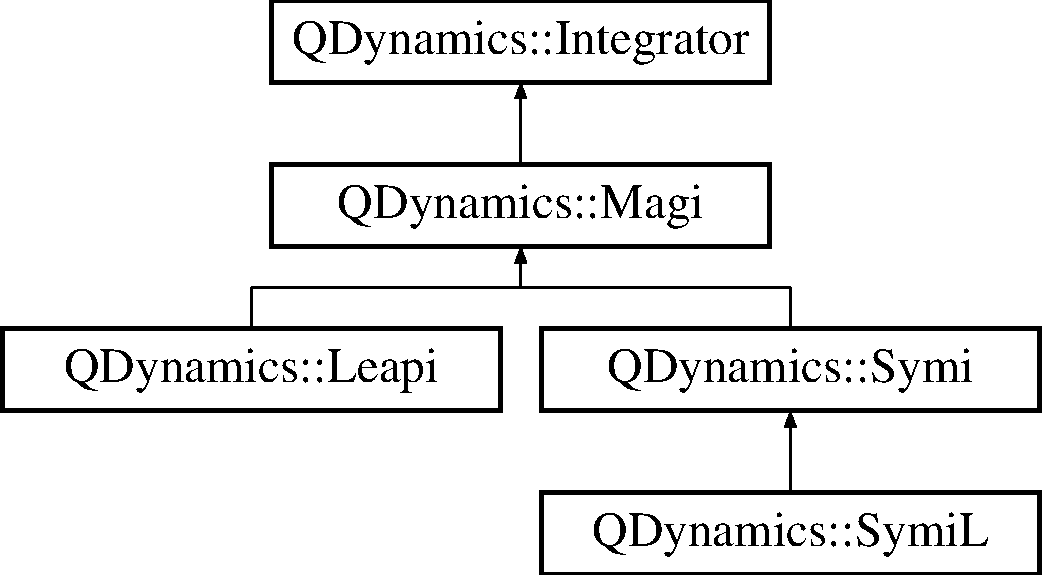
\includegraphics[height=4.000000cm]{classQDynamics_1_1Magi}
\end{center}
\end{figure}
\subsection*{Public Member Functions}
\begin{DoxyCompactItemize}
\item 
\hyperlink{classQDynamics_1_1Magi_a5b95b7c32c314e2800f59366964abfc3}{Magi} (int order, int resolution, double T, double deltaT)
\item 
\hyperlink{classQDynamics_1_1Magi_a89efe9c4722cbeb447662ee727af0570}{Magi} (int order, int resolution, double T, double deltaT, int skipper)
\end{DoxyCompactItemize}
\subsection*{Data Fields}
\begin{DoxyCompactItemize}
\item 
double \hyperlink{classQDynamics_1_1Magi_a11af2e624714857cf13343f1745f2fa8}{unlock} = 2600.\+07
\item 
bool \hyperlink{classQDynamics_1_1Magi_aba1aa111cd53a194854a2a8ac4b06b32}{unlocked} = false
\end{DoxyCompactItemize}
\subsection*{Protected Member Functions}
\begin{DoxyCompactItemize}
\item 
virtual void \hyperlink{classQDynamics_1_1Magi_a500467f899244edfae15f34c84c7684c}{Update\+Position} (double t)
\item 
virtual \hyperlink{classQDynamics_1_1Quaternion}{Quaternion} \hyperlink{classQDynamics_1_1Magi_a04b85c8aa0e9549c750956c5f781433b}{Magnus} (double duration)
\item 
virtual \hyperlink{classQDynamics_1_1Quaternion}{Quaternion} \hyperlink{classQDynamics_1_1Magi_aadacdb3581a42babd5e1aa9ada6c77ee}{Magnus\+\_\+\+Compute} (double duration)
\end{DoxyCompactItemize}
\subsection*{Protected Attributes}
\begin{DoxyCompactItemize}
\item 
const int \hyperlink{classQDynamics_1_1Magi_ac9ff1c2f4ea0dcc30f1ee52b0894c9e9}{Order}
\item 
const int \hyperlink{classQDynamics_1_1Magi_a629449f541590040a7dfb98ca68cf97b}{Resolution}
\end{DoxyCompactItemize}


\subsection{Constructor \& Destructor Documentation}
\mbox{\Hypertarget{classQDynamics_1_1Magi_a5b95b7c32c314e2800f59366964abfc3}\label{classQDynamics_1_1Magi_a5b95b7c32c314e2800f59366964abfc3}} 
\index{Q\+Dynamics\+::\+Magi@{Q\+Dynamics\+::\+Magi}!Magi@{Magi}}
\index{Magi@{Magi}!Q\+Dynamics\+::\+Magi@{Q\+Dynamics\+::\+Magi}}
\subsubsection{\texorpdfstring{Magi()}{Magi()}\hspace{0.1cm}{\footnotesize\ttfamily [1/2]}}
{\footnotesize\ttfamily Q\+Dynamics\+::\+Magi\+::\+Magi (\begin{DoxyParamCaption}\item[{int}]{order,  }\item[{int}]{resolution,  }\item[{double}]{T,  }\item[{double}]{deltaT }\end{DoxyParamCaption})\hspace{0.3cm}{\ttfamily [inline]}}

\mbox{\Hypertarget{classQDynamics_1_1Magi_a89efe9c4722cbeb447662ee727af0570}\label{classQDynamics_1_1Magi_a89efe9c4722cbeb447662ee727af0570}} 
\index{Q\+Dynamics\+::\+Magi@{Q\+Dynamics\+::\+Magi}!Magi@{Magi}}
\index{Magi@{Magi}!Q\+Dynamics\+::\+Magi@{Q\+Dynamics\+::\+Magi}}
\subsubsection{\texorpdfstring{Magi()}{Magi()}\hspace{0.1cm}{\footnotesize\ttfamily [2/2]}}
{\footnotesize\ttfamily Q\+Dynamics\+::\+Magi\+::\+Magi (\begin{DoxyParamCaption}\item[{int}]{order,  }\item[{int}]{resolution,  }\item[{double}]{T,  }\item[{double}]{deltaT,  }\item[{int}]{skipper }\end{DoxyParamCaption})\hspace{0.3cm}{\ttfamily [inline]}}



\subsection{Member Function Documentation}
\mbox{\Hypertarget{classQDynamics_1_1Magi_a04b85c8aa0e9549c750956c5f781433b}\label{classQDynamics_1_1Magi_a04b85c8aa0e9549c750956c5f781433b}} 
\index{Q\+Dynamics\+::\+Magi@{Q\+Dynamics\+::\+Magi}!Magnus@{Magnus}}
\index{Magnus@{Magnus}!Q\+Dynamics\+::\+Magi@{Q\+Dynamics\+::\+Magi}}
\subsubsection{\texorpdfstring{Magnus()}{Magnus()}}
{\footnotesize\ttfamily virtual \hyperlink{classQDynamics_1_1Quaternion}{Quaternion} Q\+Dynamics\+::\+Magi\+::\+Magnus (\begin{DoxyParamCaption}\item[{double}]{duration }\end{DoxyParamCaption})\hspace{0.3cm}{\ttfamily [inline]}, {\ttfamily [protected]}, {\ttfamily [virtual]}}

\mbox{\Hypertarget{classQDynamics_1_1Magi_aadacdb3581a42babd5e1aa9ada6c77ee}\label{classQDynamics_1_1Magi_aadacdb3581a42babd5e1aa9ada6c77ee}} 
\index{Q\+Dynamics\+::\+Magi@{Q\+Dynamics\+::\+Magi}!Magnus\+\_\+\+Compute@{Magnus\+\_\+\+Compute}}
\index{Magnus\+\_\+\+Compute@{Magnus\+\_\+\+Compute}!Q\+Dynamics\+::\+Magi@{Q\+Dynamics\+::\+Magi}}
\subsubsection{\texorpdfstring{Magnus\+\_\+\+Compute()}{Magnus\_Compute()}}
{\footnotesize\ttfamily virtual \hyperlink{classQDynamics_1_1Quaternion}{Quaternion} Q\+Dynamics\+::\+Magi\+::\+Magnus\+\_\+\+Compute (\begin{DoxyParamCaption}\item[{double}]{duration }\end{DoxyParamCaption})\hspace{0.3cm}{\ttfamily [inline]}, {\ttfamily [protected]}, {\ttfamily [virtual]}}



Reimplemented in \hyperlink{classQDynamics_1_1Symi_a4cea691ad899227f92004dd666180415}{Q\+Dynamics\+::\+Symi}.

\mbox{\Hypertarget{classQDynamics_1_1Magi_a500467f899244edfae15f34c84c7684c}\label{classQDynamics_1_1Magi_a500467f899244edfae15f34c84c7684c}} 
\index{Q\+Dynamics\+::\+Magi@{Q\+Dynamics\+::\+Magi}!Update\+Position@{Update\+Position}}
\index{Update\+Position@{Update\+Position}!Q\+Dynamics\+::\+Magi@{Q\+Dynamics\+::\+Magi}}
\subsubsection{\texorpdfstring{Update\+Position()}{UpdatePosition()}}
{\footnotesize\ttfamily virtual void Q\+Dynamics\+::\+Magi\+::\+Update\+Position (\begin{DoxyParamCaption}\item[{double}]{t }\end{DoxyParamCaption})\hspace{0.3cm}{\ttfamily [inline]}, {\ttfamily [protected]}, {\ttfamily [virtual]}}



Reimplemented from \hyperlink{classQDynamics_1_1Integrator_a4effa27d56f3205e53653b1fdc5cd08e}{Q\+Dynamics\+::\+Integrator}.



Reimplemented in \hyperlink{classQDynamics_1_1Leapi_ada2b4935513fa7e0cb4f78ade9f2fd0e}{Q\+Dynamics\+::\+Leapi}, and \hyperlink{classQDynamics_1_1SymiL_a28d23793abeb8f40c9d9ec069d67debb}{Q\+Dynamics\+::\+SymiL}.



\subsection{Field Documentation}
\mbox{\Hypertarget{classQDynamics_1_1Magi_ac9ff1c2f4ea0dcc30f1ee52b0894c9e9}\label{classQDynamics_1_1Magi_ac9ff1c2f4ea0dcc30f1ee52b0894c9e9}} 
\index{Q\+Dynamics\+::\+Magi@{Q\+Dynamics\+::\+Magi}!Order@{Order}}
\index{Order@{Order}!Q\+Dynamics\+::\+Magi@{Q\+Dynamics\+::\+Magi}}
\subsubsection{\texorpdfstring{Order}{Order}}
{\footnotesize\ttfamily const int Q\+Dynamics\+::\+Magi\+::\+Order\hspace{0.3cm}{\ttfamily [protected]}}

\mbox{\Hypertarget{classQDynamics_1_1Magi_a629449f541590040a7dfb98ca68cf97b}\label{classQDynamics_1_1Magi_a629449f541590040a7dfb98ca68cf97b}} 
\index{Q\+Dynamics\+::\+Magi@{Q\+Dynamics\+::\+Magi}!Resolution@{Resolution}}
\index{Resolution@{Resolution}!Q\+Dynamics\+::\+Magi@{Q\+Dynamics\+::\+Magi}}
\subsubsection{\texorpdfstring{Resolution}{Resolution}}
{\footnotesize\ttfamily const int Q\+Dynamics\+::\+Magi\+::\+Resolution\hspace{0.3cm}{\ttfamily [protected]}}

\mbox{\Hypertarget{classQDynamics_1_1Magi_a11af2e624714857cf13343f1745f2fa8}\label{classQDynamics_1_1Magi_a11af2e624714857cf13343f1745f2fa8}} 
\index{Q\+Dynamics\+::\+Magi@{Q\+Dynamics\+::\+Magi}!unlock@{unlock}}
\index{unlock@{unlock}!Q\+Dynamics\+::\+Magi@{Q\+Dynamics\+::\+Magi}}
\subsubsection{\texorpdfstring{unlock}{unlock}}
{\footnotesize\ttfamily double Q\+Dynamics\+::\+Magi\+::unlock = 2600.\+07}

\mbox{\Hypertarget{classQDynamics_1_1Magi_aba1aa111cd53a194854a2a8ac4b06b32}\label{classQDynamics_1_1Magi_aba1aa111cd53a194854a2a8ac4b06b32}} 
\index{Q\+Dynamics\+::\+Magi@{Q\+Dynamics\+::\+Magi}!unlocked@{unlocked}}
\index{unlocked@{unlocked}!Q\+Dynamics\+::\+Magi@{Q\+Dynamics\+::\+Magi}}
\subsubsection{\texorpdfstring{unlocked}{unlocked}}
{\footnotesize\ttfamily bool Q\+Dynamics\+::\+Magi\+::unlocked = false}



The documentation for this class was generated from the following file\+:\begin{DoxyCompactItemize}
\item 
/home/f/fraserj/\+Documents/\+Work/\+Q\+Dynamics/src/\hyperlink{Magi_8h}{Magi.\+h}\end{DoxyCompactItemize}

\hypertarget{classJSL_1_1Matrix}{}\section{J\+SL\+:\+:Matrix Class Reference}
\label{classJSL_1_1Matrix}\index{J\+S\+L\+::\+Matrix@{J\+S\+L\+::\+Matrix}}


{\ttfamily \#include $<$matrix.\+h$>$}

\subsection*{Public Member Functions}
\begin{DoxyCompactItemize}
\item 
\hyperlink{classJSL_1_1Matrix_a90ddd1113043b8959b0943be24f9ad9f}{Matrix} (const int n, const int m)
\item 
\hyperlink{classJSL_1_1Matrix_ab6bc06d3dcc5f25f2083d3a3946378df}{Matrix} (std\+::vector$<$ std\+::vector$<$ double $>$$>$ input)
\item 
\hyperlink{classJSL_1_1Matrix_ae6198f4beabaff7700265fffeb490ed7}{Matrix} (const \hyperlink{classJSL_1_1Matrix}{Matrix} \&input)
\item 
int \hyperlink{classJSL_1_1Matrix_af784cad8dcbb502c06be62e2e328ef6c}{Rows} () const
\item 
int \hyperlink{classJSL_1_1Matrix_a8aba7f9803b553df2aeae68aba3445f5}{Columns} () const
\item 
\hyperlink{classJSL_1_1Matrix}{Matrix} \hyperlink{classJSL_1_1Matrix_a984691eac759ff0e8f98252d07be7e1a}{Transpose} ()
\item 
\hyperlink{classJSL_1_1Vector}{J\+S\+L\+::\+Vector} \hyperlink{classJSL_1_1Matrix_aa8bae8650234f5e5569277563d68f22d}{Get\+Row} (int row\+ID) const
\item 
\hyperlink{classJSL_1_1Vector}{J\+S\+L\+::\+Vector} \hyperlink{classJSL_1_1Matrix_a11ea58ca43e028123f628966eb4834a0}{Get\+Column} (int col\+ID) const
\item 
double \& \hyperlink{classJSL_1_1Matrix_a23d8192e8a00d213693b82b3caeb0ceb}{operator()} (int row\+ID, int column\+ID)
\item 
const double \& \hyperlink{classJSL_1_1Matrix_ab5dd212faa491611c31288644db66a60}{operator()} (int row\+ID, int column\+ID) const
\item 
\hyperlink{classJSL_1_1Matrix}{Matrix} \& \hyperlink{classJSL_1_1Matrix_ae317e4316d0d40ce919fb22a9f4824a7}{operator+=} (const \hyperlink{classJSL_1_1Matrix}{Matrix} \&rhs)
\begin{DoxyCompactList}\small\item\em In-\/place addition of two matrices. \end{DoxyCompactList}\item 
\hyperlink{classJSL_1_1Matrix}{Matrix} \& \hyperlink{classJSL_1_1Matrix_abec89912c20210f6b49c5d09e1c1845b}{operator-\/=} (const \hyperlink{classJSL_1_1Matrix}{Matrix} \&rhs)
\begin{DoxyCompactList}\small\item\em In-\/place subtraction of two matrices. \end{DoxyCompactList}\item 
\hyperlink{classJSL_1_1Matrix}{Matrix} \& \hyperlink{classJSL_1_1Matrix_ae2dfa2fcbc80ee24c02125e5739bc0c1}{operator+=} (const double \&scalar)
\begin{DoxyCompactList}\small\item\em In-\/place addition of a scalar onto the calling object. \end{DoxyCompactList}\item 
\hyperlink{classJSL_1_1Matrix}{Matrix} \& \hyperlink{classJSL_1_1Matrix_a894ff64b1350616ddf2a48ec0f58e2c5}{operator-\/=} (const double \&scalar)
\begin{DoxyCompactList}\small\item\em In-\/place subtraction of a scalar onto the calling object. \end{DoxyCompactList}\item 
\hyperlink{classJSL_1_1Matrix}{Matrix} \& \hyperlink{classJSL_1_1Matrix_a3d9d4857ed227d7c6db87814f15af2ea}{operator$\ast$=} (const double \&scalar)
\begin{DoxyCompactList}\small\item\em In-\/place multiplication of a scalar onto the calling object. \end{DoxyCompactList}\item 
\hyperlink{classJSL_1_1Matrix}{Matrix} \& \hyperlink{classJSL_1_1Matrix_a2a9cdd54f835135496bf3e87aea4dfc9}{operator$\ast$=} (const \hyperlink{classJSL_1_1Matrix}{Matrix} \&rhs)
\item 
\hyperlink{classJSL_1_1Matrix}{Matrix} \& \hyperlink{classJSL_1_1Matrix_a6caa5725c4dacc9a841147e80e9c43a4}{operator/=} (const double \&scalar)
\begin{DoxyCompactList}\small\item\em In-\/place division of a scalar onto the calling object. \end{DoxyCompactList}\item 
std\+::string \hyperlink{classJSL_1_1Matrix_abcf44559767ab6939851f0d3b60c6fa8}{to\+\_\+string} () const
\end{DoxyCompactItemize}
\subsection*{Static Public Member Functions}
\begin{DoxyCompactItemize}
\item 
static \hyperlink{classJSL_1_1Matrix}{Matrix} \hyperlink{classJSL_1_1Matrix_afd9edd73e5f559eed02b063d4c4e47f8}{Identity} (int n)
\begin{DoxyCompactList}\small\item\em specialised psuedo-\/constructor for the identity matrix \end{DoxyCompactList}\end{DoxyCompactItemize}
\subsection*{Private Member Functions}
\begin{DoxyCompactItemize}
\item 
std\+::string \hyperlink{classJSL_1_1Matrix_a92eb431da436e1e2922b211a9f158203}{out\+Of\+Bounds\+Error} (int idx1, int idx2) const
\end{DoxyCompactItemize}
\subsection*{Private Attributes}
\begin{DoxyCompactItemize}
\item 
std\+::vector$<$ std\+::vector$<$ double $>$ $>$ \hyperlink{classJSL_1_1Matrix_a446d23ba93238f3e2dfc79a3a4d5eb7e}{Data}
\item 
int \hyperlink{classJSL_1_1Matrix_a7b7a081bbf419b613f19142a634b2cfa}{n\+Rows}
\item 
int \hyperlink{classJSL_1_1Matrix_aef59f1402d2137e86aebf6b21f97ee6d}{n\+Cols}
\end{DoxyCompactItemize}


\subsection{Constructor \& Destructor Documentation}
\mbox{\Hypertarget{classJSL_1_1Matrix_a90ddd1113043b8959b0943be24f9ad9f}\label{classJSL_1_1Matrix_a90ddd1113043b8959b0943be24f9ad9f}} 
\index{J\+S\+L\+::\+Matrix@{J\+S\+L\+::\+Matrix}!Matrix@{Matrix}}
\index{Matrix@{Matrix}!J\+S\+L\+::\+Matrix@{J\+S\+L\+::\+Matrix}}
\subsubsection{\texorpdfstring{Matrix()}{Matrix()}\hspace{0.1cm}{\footnotesize\ttfamily [1/3]}}
{\footnotesize\ttfamily J\+S\+L\+::\+Matrix\+::\+Matrix (\begin{DoxyParamCaption}\item[{const int}]{n,  }\item[{const int}]{m }\end{DoxyParamCaption})\hspace{0.3cm}{\ttfamily [inline]}}

\mbox{\Hypertarget{classJSL_1_1Matrix_ab6bc06d3dcc5f25f2083d3a3946378df}\label{classJSL_1_1Matrix_ab6bc06d3dcc5f25f2083d3a3946378df}} 
\index{J\+S\+L\+::\+Matrix@{J\+S\+L\+::\+Matrix}!Matrix@{Matrix}}
\index{Matrix@{Matrix}!J\+S\+L\+::\+Matrix@{J\+S\+L\+::\+Matrix}}
\subsubsection{\texorpdfstring{Matrix()}{Matrix()}\hspace{0.1cm}{\footnotesize\ttfamily [2/3]}}
{\footnotesize\ttfamily J\+S\+L\+::\+Matrix\+::\+Matrix (\begin{DoxyParamCaption}\item[{std\+::vector$<$ std\+::vector$<$ double $>$$>$}]{input }\end{DoxyParamCaption})\hspace{0.3cm}{\ttfamily [inline]}}

\mbox{\Hypertarget{classJSL_1_1Matrix_ae6198f4beabaff7700265fffeb490ed7}\label{classJSL_1_1Matrix_ae6198f4beabaff7700265fffeb490ed7}} 
\index{J\+S\+L\+::\+Matrix@{J\+S\+L\+::\+Matrix}!Matrix@{Matrix}}
\index{Matrix@{Matrix}!J\+S\+L\+::\+Matrix@{J\+S\+L\+::\+Matrix}}
\subsubsection{\texorpdfstring{Matrix()}{Matrix()}\hspace{0.1cm}{\footnotesize\ttfamily [3/3]}}
{\footnotesize\ttfamily J\+S\+L\+::\+Matrix\+::\+Matrix (\begin{DoxyParamCaption}\item[{const \hyperlink{classJSL_1_1Matrix}{Matrix} \&}]{input }\end{DoxyParamCaption})\hspace{0.3cm}{\ttfamily [inline]}}



\subsection{Member Function Documentation}
\mbox{\Hypertarget{classJSL_1_1Matrix_a8aba7f9803b553df2aeae68aba3445f5}\label{classJSL_1_1Matrix_a8aba7f9803b553df2aeae68aba3445f5}} 
\index{J\+S\+L\+::\+Matrix@{J\+S\+L\+::\+Matrix}!Columns@{Columns}}
\index{Columns@{Columns}!J\+S\+L\+::\+Matrix@{J\+S\+L\+::\+Matrix}}
\subsubsection{\texorpdfstring{Columns()}{Columns()}}
{\footnotesize\ttfamily int J\+S\+L\+::\+Matrix\+::\+Columns (\begin{DoxyParamCaption}{ }\end{DoxyParamCaption}) const\hspace{0.3cm}{\ttfamily [inline]}}

\mbox{\Hypertarget{classJSL_1_1Matrix_a11ea58ca43e028123f628966eb4834a0}\label{classJSL_1_1Matrix_a11ea58ca43e028123f628966eb4834a0}} 
\index{J\+S\+L\+::\+Matrix@{J\+S\+L\+::\+Matrix}!Get\+Column@{Get\+Column}}
\index{Get\+Column@{Get\+Column}!J\+S\+L\+::\+Matrix@{J\+S\+L\+::\+Matrix}}
\subsubsection{\texorpdfstring{Get\+Column()}{GetColumn()}}
{\footnotesize\ttfamily \hyperlink{classJSL_1_1Vector}{J\+S\+L\+::\+Vector} J\+S\+L\+::\+Matrix\+::\+Get\+Column (\begin{DoxyParamCaption}\item[{int}]{col\+ID }\end{DoxyParamCaption}) const\hspace{0.3cm}{\ttfamily [inline]}}

\mbox{\Hypertarget{classJSL_1_1Matrix_aa8bae8650234f5e5569277563d68f22d}\label{classJSL_1_1Matrix_aa8bae8650234f5e5569277563d68f22d}} 
\index{J\+S\+L\+::\+Matrix@{J\+S\+L\+::\+Matrix}!Get\+Row@{Get\+Row}}
\index{Get\+Row@{Get\+Row}!J\+S\+L\+::\+Matrix@{J\+S\+L\+::\+Matrix}}
\subsubsection{\texorpdfstring{Get\+Row()}{GetRow()}}
{\footnotesize\ttfamily \hyperlink{classJSL_1_1Vector}{J\+S\+L\+::\+Vector} J\+S\+L\+::\+Matrix\+::\+Get\+Row (\begin{DoxyParamCaption}\item[{int}]{row\+ID }\end{DoxyParamCaption}) const\hspace{0.3cm}{\ttfamily [inline]}}

\mbox{\Hypertarget{classJSL_1_1Matrix_afd9edd73e5f559eed02b063d4c4e47f8}\label{classJSL_1_1Matrix_afd9edd73e5f559eed02b063d4c4e47f8}} 
\index{J\+S\+L\+::\+Matrix@{J\+S\+L\+::\+Matrix}!Identity@{Identity}}
\index{Identity@{Identity}!J\+S\+L\+::\+Matrix@{J\+S\+L\+::\+Matrix}}
\subsubsection{\texorpdfstring{Identity()}{Identity()}}
{\footnotesize\ttfamily static \hyperlink{classJSL_1_1Matrix}{Matrix} J\+S\+L\+::\+Matrix\+::\+Identity (\begin{DoxyParamCaption}\item[{int}]{n }\end{DoxyParamCaption})\hspace{0.3cm}{\ttfamily [inline]}, {\ttfamily [static]}}



specialised psuedo-\/constructor for the identity matrix 

\mbox{\Hypertarget{classJSL_1_1Matrix_a23d8192e8a00d213693b82b3caeb0ceb}\label{classJSL_1_1Matrix_a23d8192e8a00d213693b82b3caeb0ceb}} 
\index{J\+S\+L\+::\+Matrix@{J\+S\+L\+::\+Matrix}!operator()@{operator()}}
\index{operator()@{operator()}!J\+S\+L\+::\+Matrix@{J\+S\+L\+::\+Matrix}}
\subsubsection{\texorpdfstring{operator()()}{operator()()}\hspace{0.1cm}{\footnotesize\ttfamily [1/2]}}
{\footnotesize\ttfamily double\& J\+S\+L\+::\+Matrix\+::operator() (\begin{DoxyParamCaption}\item[{int}]{row\+ID,  }\item[{int}]{column\+ID }\end{DoxyParamCaption})\hspace{0.3cm}{\ttfamily [inline]}}

\mbox{\Hypertarget{classJSL_1_1Matrix_ab5dd212faa491611c31288644db66a60}\label{classJSL_1_1Matrix_ab5dd212faa491611c31288644db66a60}} 
\index{J\+S\+L\+::\+Matrix@{J\+S\+L\+::\+Matrix}!operator()@{operator()}}
\index{operator()@{operator()}!J\+S\+L\+::\+Matrix@{J\+S\+L\+::\+Matrix}}
\subsubsection{\texorpdfstring{operator()()}{operator()()}\hspace{0.1cm}{\footnotesize\ttfamily [2/2]}}
{\footnotesize\ttfamily const double\& J\+S\+L\+::\+Matrix\+::operator() (\begin{DoxyParamCaption}\item[{int}]{row\+ID,  }\item[{int}]{column\+ID }\end{DoxyParamCaption}) const\hspace{0.3cm}{\ttfamily [inline]}}

\mbox{\Hypertarget{classJSL_1_1Matrix_a3d9d4857ed227d7c6db87814f15af2ea}\label{classJSL_1_1Matrix_a3d9d4857ed227d7c6db87814f15af2ea}} 
\index{J\+S\+L\+::\+Matrix@{J\+S\+L\+::\+Matrix}!operator$\ast$=@{operator$\ast$=}}
\index{operator$\ast$=@{operator$\ast$=}!J\+S\+L\+::\+Matrix@{J\+S\+L\+::\+Matrix}}
\subsubsection{\texorpdfstring{operator$\ast$=()}{operator*=()}\hspace{0.1cm}{\footnotesize\ttfamily [1/2]}}
{\footnotesize\ttfamily \hyperlink{classJSL_1_1Matrix}{Matrix}\& J\+S\+L\+::\+Matrix\+::operator$\ast$= (\begin{DoxyParamCaption}\item[{const double \&}]{scalar }\end{DoxyParamCaption})\hspace{0.3cm}{\ttfamily [inline]}}



In-\/place multiplication of a scalar onto the calling object. 


\begin{DoxyParams}{Parameters}
{\em scalar} & The double to be accumulated into the current object. \\
\hline
\end{DoxyParams}
\begin{DoxyReturn}{Returns}
A reference to the now-\/modified calling object 
\end{DoxyReturn}
\mbox{\Hypertarget{classJSL_1_1Matrix_a2a9cdd54f835135496bf3e87aea4dfc9}\label{classJSL_1_1Matrix_a2a9cdd54f835135496bf3e87aea4dfc9}} 
\index{J\+S\+L\+::\+Matrix@{J\+S\+L\+::\+Matrix}!operator$\ast$=@{operator$\ast$=}}
\index{operator$\ast$=@{operator$\ast$=}!J\+S\+L\+::\+Matrix@{J\+S\+L\+::\+Matrix}}
\subsubsection{\texorpdfstring{operator$\ast$=()}{operator*=()}\hspace{0.1cm}{\footnotesize\ttfamily [2/2]}}
{\footnotesize\ttfamily \hyperlink{classJSL_1_1Matrix}{Matrix}\& J\+S\+L\+::\+Matrix\+::operator$\ast$= (\begin{DoxyParamCaption}\item[{const \hyperlink{classJSL_1_1Matrix}{Matrix} \&}]{rhs }\end{DoxyParamCaption})\hspace{0.3cm}{\ttfamily [inline]}}

\mbox{\Hypertarget{classJSL_1_1Matrix_ae317e4316d0d40ce919fb22a9f4824a7}\label{classJSL_1_1Matrix_ae317e4316d0d40ce919fb22a9f4824a7}} 
\index{J\+S\+L\+::\+Matrix@{J\+S\+L\+::\+Matrix}!operator+=@{operator+=}}
\index{operator+=@{operator+=}!J\+S\+L\+::\+Matrix@{J\+S\+L\+::\+Matrix}}
\subsubsection{\texorpdfstring{operator+=()}{operator+=()}\hspace{0.1cm}{\footnotesize\ttfamily [1/2]}}
{\footnotesize\ttfamily \hyperlink{classJSL_1_1Matrix}{Matrix}\& J\+S\+L\+::\+Matrix\+::operator+= (\begin{DoxyParamCaption}\item[{const \hyperlink{classJSL_1_1Matrix}{Matrix} \&}]{rhs }\end{DoxyParamCaption})\hspace{0.3cm}{\ttfamily [inline]}}



In-\/place addition of two matrices. 


\begin{DoxyParams}{Parameters}
{\em rhs} & The matrix to be accumulated into the current object. Must be the same dimensions as the calling object. \\
\hline
\end{DoxyParams}
\begin{DoxyReturn}{Returns}
A reference to the now-\/modified calling object 
\end{DoxyReturn}
\mbox{\Hypertarget{classJSL_1_1Matrix_ae2dfa2fcbc80ee24c02125e5739bc0c1}\label{classJSL_1_1Matrix_ae2dfa2fcbc80ee24c02125e5739bc0c1}} 
\index{J\+S\+L\+::\+Matrix@{J\+S\+L\+::\+Matrix}!operator+=@{operator+=}}
\index{operator+=@{operator+=}!J\+S\+L\+::\+Matrix@{J\+S\+L\+::\+Matrix}}
\subsubsection{\texorpdfstring{operator+=()}{operator+=()}\hspace{0.1cm}{\footnotesize\ttfamily [2/2]}}
{\footnotesize\ttfamily \hyperlink{classJSL_1_1Matrix}{Matrix}\& J\+S\+L\+::\+Matrix\+::operator+= (\begin{DoxyParamCaption}\item[{const double \&}]{scalar }\end{DoxyParamCaption})\hspace{0.3cm}{\ttfamily [inline]}}



In-\/place addition of a scalar onto the calling object. 


\begin{DoxyParams}{Parameters}
{\em scalar} & The double to be accumulated into the current object. \\
\hline
\end{DoxyParams}
\begin{DoxyReturn}{Returns}
A reference to the now-\/modified calling object 
\end{DoxyReturn}
\mbox{\Hypertarget{classJSL_1_1Matrix_abec89912c20210f6b49c5d09e1c1845b}\label{classJSL_1_1Matrix_abec89912c20210f6b49c5d09e1c1845b}} 
\index{J\+S\+L\+::\+Matrix@{J\+S\+L\+::\+Matrix}!operator-\/=@{operator-\/=}}
\index{operator-\/=@{operator-\/=}!J\+S\+L\+::\+Matrix@{J\+S\+L\+::\+Matrix}}
\subsubsection{\texorpdfstring{operator-\/=()}{operator-=()}\hspace{0.1cm}{\footnotesize\ttfamily [1/2]}}
{\footnotesize\ttfamily \hyperlink{classJSL_1_1Matrix}{Matrix}\& J\+S\+L\+::\+Matrix\+::operator-\/= (\begin{DoxyParamCaption}\item[{const \hyperlink{classJSL_1_1Matrix}{Matrix} \&}]{rhs }\end{DoxyParamCaption})\hspace{0.3cm}{\ttfamily [inline]}}



In-\/place subtraction of two matrices. 


\begin{DoxyParams}{Parameters}
{\em rhs} & The matrix to be subtracted from the current object. Must be the same dimensions as the calling object. \\
\hline
\end{DoxyParams}
\begin{DoxyReturn}{Returns}
A reference to the now-\/modified calling object 
\end{DoxyReturn}
\mbox{\Hypertarget{classJSL_1_1Matrix_a894ff64b1350616ddf2a48ec0f58e2c5}\label{classJSL_1_1Matrix_a894ff64b1350616ddf2a48ec0f58e2c5}} 
\index{J\+S\+L\+::\+Matrix@{J\+S\+L\+::\+Matrix}!operator-\/=@{operator-\/=}}
\index{operator-\/=@{operator-\/=}!J\+S\+L\+::\+Matrix@{J\+S\+L\+::\+Matrix}}
\subsubsection{\texorpdfstring{operator-\/=()}{operator-=()}\hspace{0.1cm}{\footnotesize\ttfamily [2/2]}}
{\footnotesize\ttfamily \hyperlink{classJSL_1_1Matrix}{Matrix}\& J\+S\+L\+::\+Matrix\+::operator-\/= (\begin{DoxyParamCaption}\item[{const double \&}]{scalar }\end{DoxyParamCaption})\hspace{0.3cm}{\ttfamily [inline]}}



In-\/place subtraction of a scalar onto the calling object. 


\begin{DoxyParams}{Parameters}
{\em scalar} & The double to be subtracted from the current object. \\
\hline
\end{DoxyParams}
\begin{DoxyReturn}{Returns}
A reference to the now-\/modified calling object 
\end{DoxyReturn}
\mbox{\Hypertarget{classJSL_1_1Matrix_a6caa5725c4dacc9a841147e80e9c43a4}\label{classJSL_1_1Matrix_a6caa5725c4dacc9a841147e80e9c43a4}} 
\index{J\+S\+L\+::\+Matrix@{J\+S\+L\+::\+Matrix}!operator/=@{operator/=}}
\index{operator/=@{operator/=}!J\+S\+L\+::\+Matrix@{J\+S\+L\+::\+Matrix}}
\subsubsection{\texorpdfstring{operator/=()}{operator/=()}}
{\footnotesize\ttfamily \hyperlink{classJSL_1_1Matrix}{Matrix}\& J\+S\+L\+::\+Matrix\+::operator/= (\begin{DoxyParamCaption}\item[{const double \&}]{scalar }\end{DoxyParamCaption})\hspace{0.3cm}{\ttfamily [inline]}}



In-\/place division of a scalar onto the calling object. 


\begin{DoxyParams}{Parameters}
{\em scalar} & The double to divide the current object by. \\
\hline
\end{DoxyParams}
\begin{DoxyReturn}{Returns}
A reference to the now-\/modified calling object 
\end{DoxyReturn}
\mbox{\Hypertarget{classJSL_1_1Matrix_a92eb431da436e1e2922b211a9f158203}\label{classJSL_1_1Matrix_a92eb431da436e1e2922b211a9f158203}} 
\index{J\+S\+L\+::\+Matrix@{J\+S\+L\+::\+Matrix}!out\+Of\+Bounds\+Error@{out\+Of\+Bounds\+Error}}
\index{out\+Of\+Bounds\+Error@{out\+Of\+Bounds\+Error}!J\+S\+L\+::\+Matrix@{J\+S\+L\+::\+Matrix}}
\subsubsection{\texorpdfstring{out\+Of\+Bounds\+Error()}{outOfBoundsError()}}
{\footnotesize\ttfamily std\+::string J\+S\+L\+::\+Matrix\+::out\+Of\+Bounds\+Error (\begin{DoxyParamCaption}\item[{int}]{idx1,  }\item[{int}]{idx2 }\end{DoxyParamCaption}) const\hspace{0.3cm}{\ttfamily [inline]}, {\ttfamily [private]}}

\mbox{\Hypertarget{classJSL_1_1Matrix_af784cad8dcbb502c06be62e2e328ef6c}\label{classJSL_1_1Matrix_af784cad8dcbb502c06be62e2e328ef6c}} 
\index{J\+S\+L\+::\+Matrix@{J\+S\+L\+::\+Matrix}!Rows@{Rows}}
\index{Rows@{Rows}!J\+S\+L\+::\+Matrix@{J\+S\+L\+::\+Matrix}}
\subsubsection{\texorpdfstring{Rows()}{Rows()}}
{\footnotesize\ttfamily int J\+S\+L\+::\+Matrix\+::\+Rows (\begin{DoxyParamCaption}{ }\end{DoxyParamCaption}) const\hspace{0.3cm}{\ttfamily [inline]}}

\mbox{\Hypertarget{classJSL_1_1Matrix_abcf44559767ab6939851f0d3b60c6fa8}\label{classJSL_1_1Matrix_abcf44559767ab6939851f0d3b60c6fa8}} 
\index{J\+S\+L\+::\+Matrix@{J\+S\+L\+::\+Matrix}!to\+\_\+string@{to\+\_\+string}}
\index{to\+\_\+string@{to\+\_\+string}!J\+S\+L\+::\+Matrix@{J\+S\+L\+::\+Matrix}}
\subsubsection{\texorpdfstring{to\+\_\+string()}{to\_string()}}
{\footnotesize\ttfamily std\+::string J\+S\+L\+::\+Matrix\+::to\+\_\+string (\begin{DoxyParamCaption}{ }\end{DoxyParamCaption}) const\hspace{0.3cm}{\ttfamily [inline]}}

\mbox{\Hypertarget{classJSL_1_1Matrix_a984691eac759ff0e8f98252d07be7e1a}\label{classJSL_1_1Matrix_a984691eac759ff0e8f98252d07be7e1a}} 
\index{J\+S\+L\+::\+Matrix@{J\+S\+L\+::\+Matrix}!Transpose@{Transpose}}
\index{Transpose@{Transpose}!J\+S\+L\+::\+Matrix@{J\+S\+L\+::\+Matrix}}
\subsubsection{\texorpdfstring{Transpose()}{Transpose()}}
{\footnotesize\ttfamily \hyperlink{classJSL_1_1Matrix}{Matrix} J\+S\+L\+::\+Matrix\+::\+Transpose (\begin{DoxyParamCaption}{ }\end{DoxyParamCaption})\hspace{0.3cm}{\ttfamily [inline]}}



\subsection{Field Documentation}
\mbox{\Hypertarget{classJSL_1_1Matrix_a446d23ba93238f3e2dfc79a3a4d5eb7e}\label{classJSL_1_1Matrix_a446d23ba93238f3e2dfc79a3a4d5eb7e}} 
\index{J\+S\+L\+::\+Matrix@{J\+S\+L\+::\+Matrix}!Data@{Data}}
\index{Data@{Data}!J\+S\+L\+::\+Matrix@{J\+S\+L\+::\+Matrix}}
\subsubsection{\texorpdfstring{Data}{Data}}
{\footnotesize\ttfamily std\+::vector$<$std\+::vector$<$double$>$ $>$ J\+S\+L\+::\+Matrix\+::\+Data\hspace{0.3cm}{\ttfamily [private]}}

\mbox{\Hypertarget{classJSL_1_1Matrix_aef59f1402d2137e86aebf6b21f97ee6d}\label{classJSL_1_1Matrix_aef59f1402d2137e86aebf6b21f97ee6d}} 
\index{J\+S\+L\+::\+Matrix@{J\+S\+L\+::\+Matrix}!n\+Cols@{n\+Cols}}
\index{n\+Cols@{n\+Cols}!J\+S\+L\+::\+Matrix@{J\+S\+L\+::\+Matrix}}
\subsubsection{\texorpdfstring{n\+Cols}{nCols}}
{\footnotesize\ttfamily int J\+S\+L\+::\+Matrix\+::n\+Cols\hspace{0.3cm}{\ttfamily [private]}}

\mbox{\Hypertarget{classJSL_1_1Matrix_a7b7a081bbf419b613f19142a634b2cfa}\label{classJSL_1_1Matrix_a7b7a081bbf419b613f19142a634b2cfa}} 
\index{J\+S\+L\+::\+Matrix@{J\+S\+L\+::\+Matrix}!n\+Rows@{n\+Rows}}
\index{n\+Rows@{n\+Rows}!J\+S\+L\+::\+Matrix@{J\+S\+L\+::\+Matrix}}
\subsubsection{\texorpdfstring{n\+Rows}{nRows}}
{\footnotesize\ttfamily int J\+S\+L\+::\+Matrix\+::n\+Rows\hspace{0.3cm}{\ttfamily [private]}}



The documentation for this class was generated from the following file\+:\begin{DoxyCompactItemize}
\item 
/home/f/fraserj/\+Documents/\+Work/\+Q\+Dynamics/lib/\+J\+S\+L/\+Maths/\hyperlink{matrix_8h}{matrix.\+h}\end{DoxyCompactItemize}

\hypertarget{classJSL__Testing_1_1MatrixTest}{}\section{J\+S\+L\+\_\+\+Testing\+:\+:Matrix\+Test Class Reference}
\label{classJSL__Testing_1_1MatrixTest}\index{J\+S\+L\+\_\+\+Testing\+::\+Matrix\+Test@{J\+S\+L\+\_\+\+Testing\+::\+Matrix\+Test}}


{\ttfamily \#include $<$Testing\+\_\+\+Unit\+Tests.\+h$>$}

Inheritance diagram for J\+S\+L\+\_\+\+Testing\+:\+:Matrix\+Test\+:\begin{figure}[H]
\begin{center}
\leavevmode
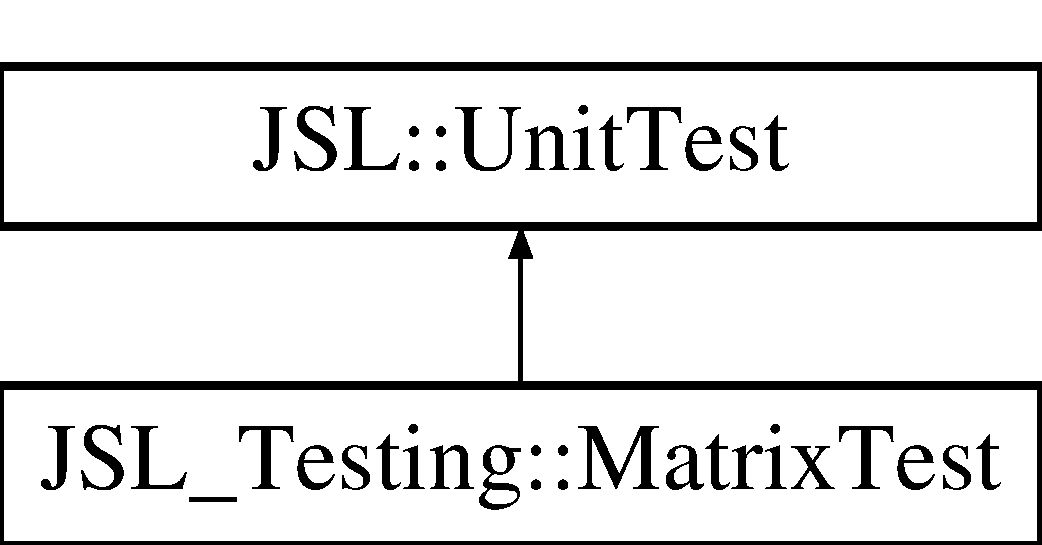
\includegraphics[height=2.000000cm]{classJSL__Testing_1_1MatrixTest}
\end{center}
\end{figure}
\subsection*{Public Member Functions}
\begin{DoxyCompactItemize}
\item 
\hyperlink{classJSL__Testing_1_1MatrixTest_a9cd56fe4c4d7db6cfd53c86252e8d033}{Matrix\+Test} ()
\item 
void \hyperlink{classJSL__Testing_1_1MatrixTest_a8fe2a671faf414dbd13c407ab52b75fb}{Run\+\_\+\+Test} ()
\begin{DoxyCompactList}\small\item\em All children which want to take advantage of the \hyperlink{classJSL_1_1UnitTest_aabec19b081be8a428f12e4b5e3dc2a9c}{Buffered\+Test()} command should have the bulk of their testing within this command. \end{DoxyCompactList}\end{DoxyCompactItemize}
\subsection*{Additional Inherited Members}


\subsection{Constructor \& Destructor Documentation}
\mbox{\Hypertarget{classJSL__Testing_1_1MatrixTest_a9cd56fe4c4d7db6cfd53c86252e8d033}\label{classJSL__Testing_1_1MatrixTest_a9cd56fe4c4d7db6cfd53c86252e8d033}} 
\index{J\+S\+L\+\_\+\+Testing\+::\+Matrix\+Test@{J\+S\+L\+\_\+\+Testing\+::\+Matrix\+Test}!Matrix\+Test@{Matrix\+Test}}
\index{Matrix\+Test@{Matrix\+Test}!J\+S\+L\+\_\+\+Testing\+::\+Matrix\+Test@{J\+S\+L\+\_\+\+Testing\+::\+Matrix\+Test}}
\subsubsection{\texorpdfstring{Matrix\+Test()}{MatrixTest()}}
{\footnotesize\ttfamily J\+S\+L\+\_\+\+Testing\+::\+Matrix\+Test\+::\+Matrix\+Test (\begin{DoxyParamCaption}{ }\end{DoxyParamCaption})\hspace{0.3cm}{\ttfamily [inline]}}



\subsection{Member Function Documentation}
\mbox{\Hypertarget{classJSL__Testing_1_1MatrixTest_a8fe2a671faf414dbd13c407ab52b75fb}\label{classJSL__Testing_1_1MatrixTest_a8fe2a671faf414dbd13c407ab52b75fb}} 
\index{J\+S\+L\+\_\+\+Testing\+::\+Matrix\+Test@{J\+S\+L\+\_\+\+Testing\+::\+Matrix\+Test}!Run\+\_\+\+Test@{Run\+\_\+\+Test}}
\index{Run\+\_\+\+Test@{Run\+\_\+\+Test}!J\+S\+L\+\_\+\+Testing\+::\+Matrix\+Test@{J\+S\+L\+\_\+\+Testing\+::\+Matrix\+Test}}
\subsubsection{\texorpdfstring{Run\+\_\+\+Test()}{Run\_Test()}}
{\footnotesize\ttfamily void J\+S\+L\+\_\+\+Testing\+::\+Matrix\+Test\+::\+Run\+\_\+\+Test (\begin{DoxyParamCaption}{ }\end{DoxyParamCaption})\hspace{0.3cm}{\ttfamily [inline]}, {\ttfamily [virtual]}}



All children which want to take advantage of the \hyperlink{classJSL_1_1UnitTest_aabec19b081be8a428f12e4b5e3dc2a9c}{Buffered\+Test()} command should have the bulk of their testing within this command. 



Reimplemented from \hyperlink{classJSL_1_1UnitTest_aa8369ab1ce2a537bff2ea7e1c8818490}{J\+S\+L\+::\+Unit\+Test}.



The documentation for this class was generated from the following file\+:\begin{DoxyCompactItemize}
\item 
/home/f/fraserj/\+Documents/\+Work/\+Q\+Dynamics/lib/\+J\+S\+L/\+Testing/\hyperlink{Testing__UnitTests_8h}{Testing\+\_\+\+Unit\+Tests.\+h}\end{DoxyCompactItemize}

\hypertarget{classJSL__Testing_1_1MetaTest}{}\section{J\+S\+L\+\_\+\+Testing\+:\+:Meta\+Test Class Reference}
\label{classJSL__Testing_1_1MetaTest}\index{J\+S\+L\+\_\+\+Testing\+::\+Meta\+Test@{J\+S\+L\+\_\+\+Testing\+::\+Meta\+Test}}


{\ttfamily \#include $<$Testing\+\_\+\+Unit\+Tests.\+h$>$}

Inheritance diagram for J\+S\+L\+\_\+\+Testing\+:\+:Meta\+Test\+:\begin{figure}[H]
\begin{center}
\leavevmode
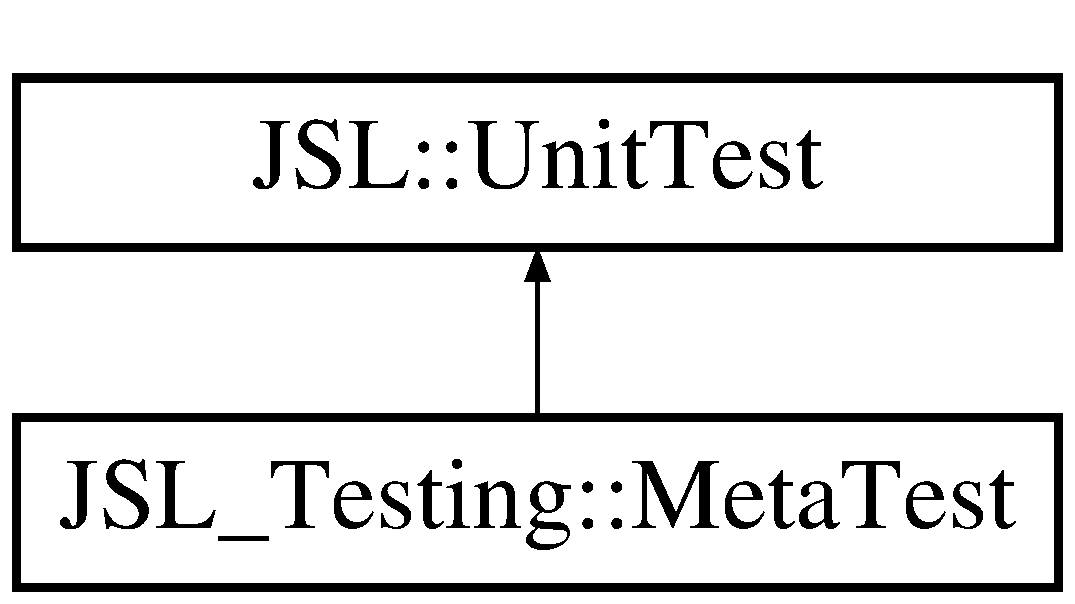
\includegraphics[height=2.000000cm]{classJSL__Testing_1_1MetaTest}
\end{center}
\end{figure}
\subsection*{Public Member Functions}
\begin{DoxyCompactItemize}
\item 
\hyperlink{classJSL__Testing_1_1MetaTest_a17efe6a92ae4934828a61d9f1120e67d}{Meta\+Test} ()
\item 
void \hyperlink{classJSL__Testing_1_1MetaTest_a176352dcd54f9ec7df8f1548882e6820}{Run\+\_\+\+Test} ()
\begin{DoxyCompactList}\small\item\em All children which want to take advantage of the \hyperlink{classJSL_1_1UnitTest_aabec19b081be8a428f12e4b5e3dc2a9c}{Buffered\+Test()} command should have the bulk of their testing within this command. \end{DoxyCompactList}\end{DoxyCompactItemize}
\subsection*{Additional Inherited Members}


\subsection{Constructor \& Destructor Documentation}
\mbox{\Hypertarget{classJSL__Testing_1_1MetaTest_a17efe6a92ae4934828a61d9f1120e67d}\label{classJSL__Testing_1_1MetaTest_a17efe6a92ae4934828a61d9f1120e67d}} 
\index{J\+S\+L\+\_\+\+Testing\+::\+Meta\+Test@{J\+S\+L\+\_\+\+Testing\+::\+Meta\+Test}!Meta\+Test@{Meta\+Test}}
\index{Meta\+Test@{Meta\+Test}!J\+S\+L\+\_\+\+Testing\+::\+Meta\+Test@{J\+S\+L\+\_\+\+Testing\+::\+Meta\+Test}}
\subsubsection{\texorpdfstring{Meta\+Test()}{MetaTest()}}
{\footnotesize\ttfamily J\+S\+L\+\_\+\+Testing\+::\+Meta\+Test\+::\+Meta\+Test (\begin{DoxyParamCaption}{ }\end{DoxyParamCaption})\hspace{0.3cm}{\ttfamily [inline]}}



\subsection{Member Function Documentation}
\mbox{\Hypertarget{classJSL__Testing_1_1MetaTest_a176352dcd54f9ec7df8f1548882e6820}\label{classJSL__Testing_1_1MetaTest_a176352dcd54f9ec7df8f1548882e6820}} 
\index{J\+S\+L\+\_\+\+Testing\+::\+Meta\+Test@{J\+S\+L\+\_\+\+Testing\+::\+Meta\+Test}!Run\+\_\+\+Test@{Run\+\_\+\+Test}}
\index{Run\+\_\+\+Test@{Run\+\_\+\+Test}!J\+S\+L\+\_\+\+Testing\+::\+Meta\+Test@{J\+S\+L\+\_\+\+Testing\+::\+Meta\+Test}}
\subsubsection{\texorpdfstring{Run\+\_\+\+Test()}{Run\_Test()}}
{\footnotesize\ttfamily void J\+S\+L\+\_\+\+Testing\+::\+Meta\+Test\+::\+Run\+\_\+\+Test (\begin{DoxyParamCaption}{ }\end{DoxyParamCaption})\hspace{0.3cm}{\ttfamily [inline]}, {\ttfamily [virtual]}}



All children which want to take advantage of the \hyperlink{classJSL_1_1UnitTest_aabec19b081be8a428f12e4b5e3dc2a9c}{Buffered\+Test()} command should have the bulk of their testing within this command. 



Reimplemented from \hyperlink{classJSL_1_1UnitTest_aa8369ab1ce2a537bff2ea7e1c8818490}{J\+S\+L\+::\+Unit\+Test}.



The documentation for this class was generated from the following file\+:\begin{DoxyCompactItemize}
\item 
/home/f/fraserj/\+Documents/\+Work/\+Q\+Dynamics/lib/\+J\+S\+L/\+Testing/\hyperlink{Testing__UnitTests_8h}{Testing\+\_\+\+Unit\+Tests.\+h}\end{DoxyCompactItemize}

\hypertarget{structJSL_1_1mkdirReturn}{}\doxysection{J\+SL\+::mkdir\+Return Struct Reference}
\label{structJSL_1_1mkdirReturn}\index{JSL::mkdirReturn@{JSL::mkdirReturn}}


A wrapper for the return type of mkdir\+Safely()  




{\ttfamily \#include $<$mkdir.\+h$>$}

\doxysubsection*{Data Fields}
\begin{DoxyCompactItemize}
\item 
bool \mbox{\hyperlink{structJSL_1_1mkdirReturn_a76abe5af61a20e13756f833b79782b7f}{Successful}}
\begin{DoxyCompactList}\small\item\em True if the directory already existed, or was succesfully created. \end{DoxyCompactList}\item 
std\+::string \mbox{\hyperlink{structJSL_1_1mkdirReturn_a64650d2f4b3d2ca29de3a4dcfdadbd0e}{Message}}
\begin{DoxyCompactList}\small\item\em Contains the logging messages from the function. \end{DoxyCompactList}\end{DoxyCompactItemize}


\doxysubsection{Detailed Description}
A wrapper for the return type of mkdir\+Safely() 

\doxysubsection{Field Documentation}
\mbox{\Hypertarget{structJSL_1_1mkdirReturn_a64650d2f4b3d2ca29de3a4dcfdadbd0e}\label{structJSL_1_1mkdirReturn_a64650d2f4b3d2ca29de3a4dcfdadbd0e}} 
\index{JSL::mkdirReturn@{JSL::mkdirReturn}!Message@{Message}}
\index{Message@{Message}!JSL::mkdirReturn@{JSL::mkdirReturn}}
\doxysubsubsection{\texorpdfstring{Message}{Message}}
{\footnotesize\ttfamily std\+::string J\+S\+L\+::mkdir\+Return\+::\+Message}



Contains the logging messages from the function. 

\mbox{\Hypertarget{structJSL_1_1mkdirReturn_a76abe5af61a20e13756f833b79782b7f}\label{structJSL_1_1mkdirReturn_a76abe5af61a20e13756f833b79782b7f}} 
\index{JSL::mkdirReturn@{JSL::mkdirReturn}!Successful@{Successful}}
\index{Successful@{Successful}!JSL::mkdirReturn@{JSL::mkdirReturn}}
\doxysubsubsection{\texorpdfstring{Successful}{Successful}}
{\footnotesize\ttfamily bool J\+S\+L\+::mkdir\+Return\+::\+Successful}



True if the directory already existed, or was succesfully created. 



The documentation for this struct was generated from the following file\+:\begin{DoxyCompactItemize}
\item 
/home/jack/\+Documents/\+Work/\+Q\+Dynamics/lib/\+J\+S\+L/\+File\+I\+O/\mbox{\hyperlink{mkdir_8h}{mkdir.\+h}}\end{DoxyCompactItemize}

\hypertarget{classQDynamics_1_1Quaternion}{}\doxysection{Q\+Dynamics\+::Quaternion Class Reference}
\label{classQDynamics_1_1Quaternion}\index{QDynamics::Quaternion@{QDynamics::Quaternion}}


{\ttfamily \#include $<$Quaternion.\+h$>$}

Inheritance diagram for Q\+Dynamics\+::Quaternion\+:\begin{figure}[H]
\begin{center}
\leavevmode
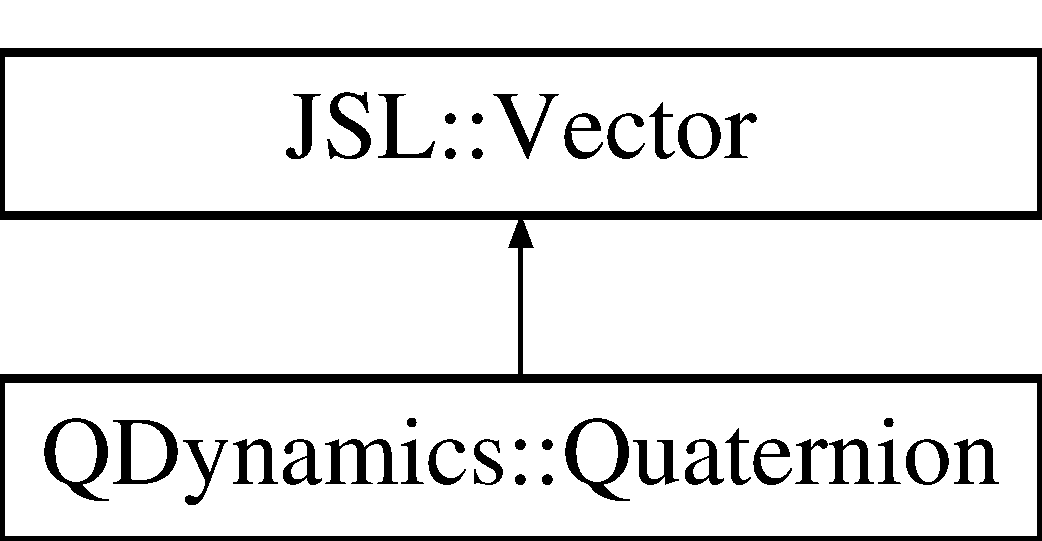
\includegraphics[height=2.000000cm]{classQDynamics_1_1Quaternion}
\end{center}
\end{figure}
\doxysubsection*{Public Member Functions}
\begin{DoxyCompactItemize}
\item 
double \& \mbox{\hyperlink{classQDynamics_1_1Quaternion_a8121c47a579baffb9e692b8cd2c7dee7}{Scalar}} ()
\begin{DoxyCompactList}\small\item\em The current value of the Scalar component, returned as a {\itshape reference}. This allows it to be assigned to\+: q.\+Scalar() = x stores the value of x in the scalar component. \end{DoxyCompactList}\item 
double \& \mbox{\hyperlink{classQDynamics_1_1Quaternion_ad2f24d575d2fb8a50a9d4fd397115b9e}{Vector}} (int i)
\begin{DoxyCompactList}\small\item\em The current value of the ith Vector component, returned as a {\itshape reference}. This allows it to be assigned to\+: q.\+Vector(i) = x stores the value of x in the scalar component. \end{DoxyCompactList}\item 
\mbox{\hyperlink{classJSL_1_1Vector}{J\+S\+L\+::\+Vector}} \mbox{\hyperlink{classQDynamics_1_1Quaternion_ac35047116c055b5baeec49b8ebba0ede}{Vector}} () const
\begin{DoxyCompactList}\small\item\em The current value of the Vector component. This cannot be modified in-\/place or assigned to as \mbox{\hyperlink{classQDynamics_1_1Quaternion_ad2f24d575d2fb8a50a9d4fd397115b9e}{Vector(int i)}} and \mbox{\hyperlink{classQDynamics_1_1Quaternion_a8121c47a579baffb9e692b8cd2c7dee7}{Scalar()}} can be. \end{DoxyCompactList}\item 
\mbox{\hyperlink{classQDynamics_1_1Quaternion_addca2bd1d2288c6875eab9f7b4c60881}{Quaternion}} ()
\begin{DoxyCompactList}\small\item\em Default initialiser. Initialises to. \end{DoxyCompactList}\item 
\mbox{\hyperlink{classQDynamics_1_1Quaternion_a206147a6dbe4a9456cd655d654ef0182}{Quaternion}} (const double \&q0, const \mbox{\hyperlink{classJSL_1_1Vector}{J\+S\+L\+::\+Vector}} \&q\+Vec)
\begin{DoxyCompactList}\small\item\em Initialises the object to. \end{DoxyCompactList}\item 
\mbox{\hyperlink{classQDynamics_1_1Quaternion_aadf267f7d62df09bf09b04cc47704560}{Quaternion}} (const double \&a, const double \&b, const double \&c, const double \&d)
\begin{DoxyCompactList}\small\item\em Initialises the object to the value. \end{DoxyCompactList}\item 
\mbox{\hyperlink{classQDynamics_1_1Quaternion_a0a153753fb53bf466a5b1c6ab20abff6}{Quaternion}} (const \mbox{\hyperlink{classJSL_1_1Vector}{J\+S\+L\+::\+Vector}} \&vec4)
\begin{DoxyCompactList}\small\item\em Initialises the quaternion as if it were a member of R$^\wedge$4. \end{DoxyCompactList}\item 
\mbox{\hyperlink{classQDynamics_1_1Quaternion_ad0da33a229eb9869a4b48c8302f5470e}{Quaternion}} (const std\+::vector$<$ double $>$ \&vec4)
\begin{DoxyCompactList}\small\item\em Initialises the quaternion as if it were a member of R$^\wedge$4. \end{DoxyCompactList}\item 
\mbox{\hyperlink{classQDynamics_1_1Quaternion}{Quaternion}} \mbox{\hyperlink{classQDynamics_1_1Quaternion_a2516e87ebb14ee2d34bc22744057c87b}{Conjugate}} () const
\begin{DoxyCompactList}\small\item\em Returns the conjugate of the current quaternion. \end{DoxyCompactList}\item 
\mbox{\hyperlink{classJSL_1_1Matrix}{J\+S\+L\+::\+Matrix}} \mbox{\hyperlink{classQDynamics_1_1Quaternion_a2d0f1e0e8e46d1223f848da4f8b3fc2e}{Left\+Multiplication\+Matrix}} () const
\begin{DoxyCompactList}\small\item\em Constructs a matrix L(q) such that L(q) b = q$\ast$b, replacing the usual quaternion multiplication operation \mbox{\hyperlink{namespaceQDynamics_ac40010112506831ced816640def9bc85}{operator$\ast$(const Quaternion \& lhs, const Quaternion \& rhs)}} \end{DoxyCompactList}\item 
\mbox{\hyperlink{classJSL_1_1Matrix}{J\+S\+L\+::\+Matrix}} \mbox{\hyperlink{classQDynamics_1_1Quaternion_a76da0390b336de90b27e713c34a3732a}{Right\+Multiplication\+Matrix}} () const
\begin{DoxyCompactList}\small\item\em Constructs a matrix R(q) such that R(q) b = b$\ast$q, replacing the usual quaternion multiplication operation \mbox{\hyperlink{namespaceQDynamics_ac40010112506831ced816640def9bc85}{operator$\ast$(const Quaternion \& lhs, const Quaternion \& rhs)}} \end{DoxyCompactList}\item 
const double \& \mbox{\hyperlink{classQDynamics_1_1Quaternion_a1bc0af90c699e7c2eba94833ae7fb105}{Scalar}} () const
\begin{DoxyCompactList}\small\item\em An annoying double-\/definition of \mbox{\hyperlink{classQDynamics_1_1Quaternion_a8121c47a579baffb9e692b8cd2c7dee7}{Scalar()}}, required for when the quaternion object is a const (and hence the references need to be carefully guarded) \end{DoxyCompactList}\item 
const double \& \mbox{\hyperlink{classQDynamics_1_1Quaternion_a061cd74a6e060beeeb781b6cf7b7f16d}{Vector}} (int id) const
\begin{DoxyCompactList}\small\item\em An annoying double-\/definition of Scalar(int i), required for when the quaternion object is a const (and hence the references need to be carefully guarded) \end{DoxyCompactList}\end{DoxyCompactItemize}
\doxysubsection*{Static Public Member Functions}
\begin{DoxyCompactItemize}
\item 
static \mbox{\hyperlink{classQDynamics_1_1Quaternion}{Quaternion}} \mbox{\hyperlink{classQDynamics_1_1Quaternion_a06726eb02ffd68ccbd3adaef63c90bb9}{One}} ()
\begin{DoxyCompactList}\small\item\em A static constructor which returns the multiplicative identity. \end{DoxyCompactList}\item 
static \mbox{\hyperlink{classQDynamics_1_1Quaternion}{Quaternion}} \mbox{\hyperlink{classQDynamics_1_1Quaternion_a7932eeb535080e6230e98fb4f35867c2}{Zero}} ()
\begin{DoxyCompactList}\small\item\em A static constructor which returns the additive identity. \end{DoxyCompactList}\item 
static \mbox{\hyperlink{classQDynamics_1_1Quaternion}{Quaternion}} \mbox{\hyperlink{classQDynamics_1_1Quaternion_a06386710ec4308c04a72f365382472ce}{Random}} ()
\begin{DoxyCompactList}\small\item\em Generates a quaternion which is randomly populated with values between 0 and 1. \end{DoxyCompactList}\end{DoxyCompactItemize}
\doxysubsection*{Additional Inherited Members}


\doxysubsection{Detailed Description}
A computational replica of the mathematical object {\itshape quaternion}, which replicates the expected behaviour of such objects, including addition and scalar multiplication (which it inherits from\begin{DoxyVerb}embed:rst:inline `JSL::Vector() <https://jackstandardlibrary.readthedocs.io/en/latest/vectors.html>`_ \end{DoxyVerb}
 ), as well as the idiosyncratic multiplication and division native ot this field. We use the notation that\begin{DoxyVerb}embed:rst:inline :math:`\mathsf{q} = (q_0, \vec{q})` \end{DoxyVerb}
 , and the interface is based on this assumption. It is intentional that treating quaternions as members of\begin{DoxyVerb}embed:rst:inline :math:`\mathbb{R}^4` \end{DoxyVerb}
 is awkward. 

\doxysubsection{Constructor \& Destructor Documentation}
\mbox{\Hypertarget{classQDynamics_1_1Quaternion_addca2bd1d2288c6875eab9f7b4c60881}\label{classQDynamics_1_1Quaternion_addca2bd1d2288c6875eab9f7b4c60881}} 
\index{QDynamics::Quaternion@{QDynamics::Quaternion}!Quaternion@{Quaternion}}
\index{Quaternion@{Quaternion}!QDynamics::Quaternion@{QDynamics::Quaternion}}
\doxysubsubsection{\texorpdfstring{Quaternion()}{Quaternion()}\hspace{0.1cm}{\footnotesize\ttfamily [1/5]}}
{\footnotesize\ttfamily Q\+Dynamics\+::\+Quaternion\+::\+Quaternion (\begin{DoxyParamCaption}{ }\end{DoxyParamCaption})\hspace{0.3cm}{\ttfamily [inline]}}



Default initialiser. Initialises to. 

\begin{DoxyVerb}embed:rst:inline :math:`\mathsf{q} = (0, \vec{0})` \end{DoxyVerb}
 \mbox{\Hypertarget{classQDynamics_1_1Quaternion_a206147a6dbe4a9456cd655d654ef0182}\label{classQDynamics_1_1Quaternion_a206147a6dbe4a9456cd655d654ef0182}} 
\index{QDynamics::Quaternion@{QDynamics::Quaternion}!Quaternion@{Quaternion}}
\index{Quaternion@{Quaternion}!QDynamics::Quaternion@{QDynamics::Quaternion}}
\doxysubsubsection{\texorpdfstring{Quaternion()}{Quaternion()}\hspace{0.1cm}{\footnotesize\ttfamily [2/5]}}
{\footnotesize\ttfamily Q\+Dynamics\+::\+Quaternion\+::\+Quaternion (\begin{DoxyParamCaption}\item[{const double \&}]{q0,  }\item[{const \mbox{\hyperlink{classJSL_1_1Vector}{J\+S\+L\+::\+Vector}} \&}]{q\+Vec }\end{DoxyParamCaption})\hspace{0.3cm}{\ttfamily [inline]}}



Initialises the object to. 

\begin{DoxyVerb}embed:rst:inline :math:`\mathsf{q} = (q_0, \vec{q})` \end{DoxyVerb}

\begin{DoxyParams}{Parameters}
{\em q0} & The value\begin{DoxyVerb}embed:rst:inline :math:`q_0` \end{DoxyVerb}
\\
\hline
{\em q\+Vec} & The value\begin{DoxyVerb}embed:rst:inline :math:`\vec{q}` \end{DoxyVerb}
. This must be a vector of length 3, or an error is thrown. \\
\hline
\end{DoxyParams}
\mbox{\Hypertarget{classQDynamics_1_1Quaternion_aadf267f7d62df09bf09b04cc47704560}\label{classQDynamics_1_1Quaternion_aadf267f7d62df09bf09b04cc47704560}} 
\index{QDynamics::Quaternion@{QDynamics::Quaternion}!Quaternion@{Quaternion}}
\index{Quaternion@{Quaternion}!QDynamics::Quaternion@{QDynamics::Quaternion}}
\doxysubsubsection{\texorpdfstring{Quaternion()}{Quaternion()}\hspace{0.1cm}{\footnotesize\ttfamily [3/5]}}
{\footnotesize\ttfamily Q\+Dynamics\+::\+Quaternion\+::\+Quaternion (\begin{DoxyParamCaption}\item[{const double \&}]{a,  }\item[{const double \&}]{b,  }\item[{const double \&}]{c,  }\item[{const double \&}]{d }\end{DoxyParamCaption})\hspace{0.3cm}{\ttfamily [inline]}}



Initialises the object to the value. 

\begin{DoxyVerb}embed:rst:inline :math:`\mathsf{q} = \left(a, \begin{pmatrix} b \\ c \\ d \end{pmatrix}\right)` \end{DoxyVerb}

\begin{DoxyParams}{Parameters}
{\em a} & The scalar value of the quaternion\\
\hline
{\em b} & The x-\/component of the vector\\
\hline
{\em c} & The y-\/component of the vector\\
\hline
{\em d} & The z-\/component of the vector \\
\hline
\end{DoxyParams}
\mbox{\Hypertarget{classQDynamics_1_1Quaternion_a0a153753fb53bf466a5b1c6ab20abff6}\label{classQDynamics_1_1Quaternion_a0a153753fb53bf466a5b1c6ab20abff6}} 
\index{QDynamics::Quaternion@{QDynamics::Quaternion}!Quaternion@{Quaternion}}
\index{Quaternion@{Quaternion}!QDynamics::Quaternion@{QDynamics::Quaternion}}
\doxysubsubsection{\texorpdfstring{Quaternion()}{Quaternion()}\hspace{0.1cm}{\footnotesize\ttfamily [4/5]}}
{\footnotesize\ttfamily Q\+Dynamics\+::\+Quaternion\+::\+Quaternion (\begin{DoxyParamCaption}\item[{const \mbox{\hyperlink{classJSL_1_1Vector}{J\+S\+L\+::\+Vector}} \&}]{vec4 }\end{DoxyParamCaption})\hspace{0.3cm}{\ttfamily [inline]}}



Initialises the quaternion as if it were a member of R$^\wedge$4. 


\begin{DoxyParams}{Parameters}
{\em vec4} & A \mbox{\hyperlink{classJSL_1_1Vector}{J\+S\+L\+::\+Vector}} object of length 4 (else an error is thrown) \\
\hline
\end{DoxyParams}
\mbox{\Hypertarget{classQDynamics_1_1Quaternion_ad0da33a229eb9869a4b48c8302f5470e}\label{classQDynamics_1_1Quaternion_ad0da33a229eb9869a4b48c8302f5470e}} 
\index{QDynamics::Quaternion@{QDynamics::Quaternion}!Quaternion@{Quaternion}}
\index{Quaternion@{Quaternion}!QDynamics::Quaternion@{QDynamics::Quaternion}}
\doxysubsubsection{\texorpdfstring{Quaternion()}{Quaternion()}\hspace{0.1cm}{\footnotesize\ttfamily [5/5]}}
{\footnotesize\ttfamily Q\+Dynamics\+::\+Quaternion\+::\+Quaternion (\begin{DoxyParamCaption}\item[{const std\+::vector$<$ double $>$ \&}]{vec4 }\end{DoxyParamCaption})\hspace{0.3cm}{\ttfamily [inline]}}



Initialises the quaternion as if it were a member of R$^\wedge$4. 


\begin{DoxyParams}{Parameters}
{\em vec4} & A std\+::vector$<$double$>$ object of length 4 (else an error is thrown) \\
\hline
\end{DoxyParams}


\doxysubsection{Member Function Documentation}
\mbox{\Hypertarget{classQDynamics_1_1Quaternion_a2516e87ebb14ee2d34bc22744057c87b}\label{classQDynamics_1_1Quaternion_a2516e87ebb14ee2d34bc22744057c87b}} 
\index{QDynamics::Quaternion@{QDynamics::Quaternion}!Conjugate@{Conjugate}}
\index{Conjugate@{Conjugate}!QDynamics::Quaternion@{QDynamics::Quaternion}}
\doxysubsubsection{\texorpdfstring{Conjugate()}{Conjugate()}}
{\footnotesize\ttfamily \mbox{\hyperlink{classQDynamics_1_1Quaternion}{Quaternion}} Q\+Dynamics\+::\+Quaternion\+::\+Conjugate (\begin{DoxyParamCaption}{ }\end{DoxyParamCaption}) const\hspace{0.3cm}{\ttfamily [inline]}}



Returns the conjugate of the current quaternion. 

\begin{DoxyReturn}{Returns}
The value\begin{DoxyVerb}embed:rst:inline :math:`\overline{\mathsf{q}} = (q_0, -\vec{q})` \end{DoxyVerb}
 
\end{DoxyReturn}
\mbox{\Hypertarget{classQDynamics_1_1Quaternion_a2d0f1e0e8e46d1223f848da4f8b3fc2e}\label{classQDynamics_1_1Quaternion_a2d0f1e0e8e46d1223f848da4f8b3fc2e}} 
\index{QDynamics::Quaternion@{QDynamics::Quaternion}!LeftMultiplicationMatrix@{LeftMultiplicationMatrix}}
\index{LeftMultiplicationMatrix@{LeftMultiplicationMatrix}!QDynamics::Quaternion@{QDynamics::Quaternion}}
\doxysubsubsection{\texorpdfstring{LeftMultiplicationMatrix()}{LeftMultiplicationMatrix()}}
{\footnotesize\ttfamily \mbox{\hyperlink{classJSL_1_1Matrix}{J\+S\+L\+::\+Matrix}} Q\+Dynamics\+::\+Quaternion\+::\+Left\+Multiplication\+Matrix (\begin{DoxyParamCaption}{ }\end{DoxyParamCaption}) const\hspace{0.3cm}{\ttfamily [inline]}}



Constructs a matrix L(q) such that L(q) b = q$\ast$b, replacing the usual quaternion multiplication operation \mbox{\hyperlink{namespaceQDynamics_ac40010112506831ced816640def9bc85}{operator$\ast$(const Quaternion \& lhs, const Quaternion \& rhs)}} 

\begin{DoxyReturn}{Returns}
The \mbox{\hyperlink{classJSL_1_1Matrix}{J\+S\+L\+::\+Matrix}} object which performs the multiplication 
\end{DoxyReturn}
\mbox{\Hypertarget{classQDynamics_1_1Quaternion_a06726eb02ffd68ccbd3adaef63c90bb9}\label{classQDynamics_1_1Quaternion_a06726eb02ffd68ccbd3adaef63c90bb9}} 
\index{QDynamics::Quaternion@{QDynamics::Quaternion}!One@{One}}
\index{One@{One}!QDynamics::Quaternion@{QDynamics::Quaternion}}
\doxysubsubsection{\texorpdfstring{One()}{One()}}
{\footnotesize\ttfamily static \mbox{\hyperlink{classQDynamics_1_1Quaternion}{Quaternion}} Q\+Dynamics\+::\+Quaternion\+::\+One (\begin{DoxyParamCaption}{ }\end{DoxyParamCaption})\hspace{0.3cm}{\ttfamily [inline]}, {\ttfamily [static]}}



A static constructor which returns the multiplicative identity. 

\begin{DoxyVerb}embed:rst:inline :math:`\mathsf{q} = \left(1, \vec{0}\right)` \end{DoxyVerb}
 \mbox{\Hypertarget{classQDynamics_1_1Quaternion_a06386710ec4308c04a72f365382472ce}\label{classQDynamics_1_1Quaternion_a06386710ec4308c04a72f365382472ce}} 
\index{QDynamics::Quaternion@{QDynamics::Quaternion}!Random@{Random}}
\index{Random@{Random}!QDynamics::Quaternion@{QDynamics::Quaternion}}
\doxysubsubsection{\texorpdfstring{Random()}{Random()}}
{\footnotesize\ttfamily static \mbox{\hyperlink{classQDynamics_1_1Quaternion}{Quaternion}} Q\+Dynamics\+::\+Quaternion\+::\+Random (\begin{DoxyParamCaption}{ }\end{DoxyParamCaption})\hspace{0.3cm}{\ttfamily [inline]}, {\ttfamily [static]}}



Generates a quaternion which is randomly populated with values between 0 and 1. 

\mbox{\Hypertarget{classQDynamics_1_1Quaternion_a76da0390b336de90b27e713c34a3732a}\label{classQDynamics_1_1Quaternion_a76da0390b336de90b27e713c34a3732a}} 
\index{QDynamics::Quaternion@{QDynamics::Quaternion}!RightMultiplicationMatrix@{RightMultiplicationMatrix}}
\index{RightMultiplicationMatrix@{RightMultiplicationMatrix}!QDynamics::Quaternion@{QDynamics::Quaternion}}
\doxysubsubsection{\texorpdfstring{RightMultiplicationMatrix()}{RightMultiplicationMatrix()}}
{\footnotesize\ttfamily \mbox{\hyperlink{classJSL_1_1Matrix}{J\+S\+L\+::\+Matrix}} Q\+Dynamics\+::\+Quaternion\+::\+Right\+Multiplication\+Matrix (\begin{DoxyParamCaption}{ }\end{DoxyParamCaption}) const\hspace{0.3cm}{\ttfamily [inline]}}



Constructs a matrix R(q) such that R(q) b = b$\ast$q, replacing the usual quaternion multiplication operation \mbox{\hyperlink{namespaceQDynamics_ac40010112506831ced816640def9bc85}{operator$\ast$(const Quaternion \& lhs, const Quaternion \& rhs)}} 

\begin{DoxyReturn}{Returns}
The \mbox{\hyperlink{classJSL_1_1Matrix}{J\+S\+L\+::\+Matrix}} object which performs the multiplication 
\end{DoxyReturn}
\mbox{\Hypertarget{classQDynamics_1_1Quaternion_a8121c47a579baffb9e692b8cd2c7dee7}\label{classQDynamics_1_1Quaternion_a8121c47a579baffb9e692b8cd2c7dee7}} 
\index{QDynamics::Quaternion@{QDynamics::Quaternion}!Scalar@{Scalar}}
\index{Scalar@{Scalar}!QDynamics::Quaternion@{QDynamics::Quaternion}}
\doxysubsubsection{\texorpdfstring{Scalar()}{Scalar()}\hspace{0.1cm}{\footnotesize\ttfamily [1/2]}}
{\footnotesize\ttfamily double\& Q\+Dynamics\+::\+Quaternion\+::\+Scalar (\begin{DoxyParamCaption}{ }\end{DoxyParamCaption})\hspace{0.3cm}{\ttfamily [inline]}}



The current value of the Scalar component, returned as a {\itshape reference}. This allows it to be assigned to\+: q.\+Scalar() = x stores the value of x in the scalar component. 

\begin{DoxyReturn}{Returns}
A reference to the scalar component of the quaternion 
\end{DoxyReturn}
\mbox{\Hypertarget{classQDynamics_1_1Quaternion_a1bc0af90c699e7c2eba94833ae7fb105}\label{classQDynamics_1_1Quaternion_a1bc0af90c699e7c2eba94833ae7fb105}} 
\index{QDynamics::Quaternion@{QDynamics::Quaternion}!Scalar@{Scalar}}
\index{Scalar@{Scalar}!QDynamics::Quaternion@{QDynamics::Quaternion}}
\doxysubsubsection{\texorpdfstring{Scalar()}{Scalar()}\hspace{0.1cm}{\footnotesize\ttfamily [2/2]}}
{\footnotesize\ttfamily const double\& Q\+Dynamics\+::\+Quaternion\+::\+Scalar (\begin{DoxyParamCaption}{ }\end{DoxyParamCaption}) const\hspace{0.3cm}{\ttfamily [inline]}}



An annoying double-\/definition of \mbox{\hyperlink{classQDynamics_1_1Quaternion_a8121c47a579baffb9e692b8cd2c7dee7}{Scalar()}}, required for when the quaternion object is a const (and hence the references need to be carefully guarded) 

\mbox{\Hypertarget{classQDynamics_1_1Quaternion_ac35047116c055b5baeec49b8ebba0ede}\label{classQDynamics_1_1Quaternion_ac35047116c055b5baeec49b8ebba0ede}} 
\index{QDynamics::Quaternion@{QDynamics::Quaternion}!Vector@{Vector}}
\index{Vector@{Vector}!QDynamics::Quaternion@{QDynamics::Quaternion}}
\doxysubsubsection{\texorpdfstring{Vector()}{Vector()}\hspace{0.1cm}{\footnotesize\ttfamily [1/3]}}
{\footnotesize\ttfamily \mbox{\hyperlink{classJSL_1_1Vector}{J\+S\+L\+::\+Vector}} Q\+Dynamics\+::\+Quaternion\+::\+Vector (\begin{DoxyParamCaption}{ }\end{DoxyParamCaption}) const\hspace{0.3cm}{\ttfamily [inline]}}



The current value of the Vector component. This cannot be modified in-\/place or assigned to as \mbox{\hyperlink{classQDynamics_1_1Quaternion_ad2f24d575d2fb8a50a9d4fd397115b9e}{Vector(int i)}} and \mbox{\hyperlink{classQDynamics_1_1Quaternion_a8121c47a579baffb9e692b8cd2c7dee7}{Scalar()}} can be. 

\begin{DoxyReturn}{Returns}
A \mbox{\hyperlink{classJSL_1_1Vector}{J\+S\+L\+::\+Vector}} object containing the Vector portion of the quaternion. 
\end{DoxyReturn}
\mbox{\Hypertarget{classQDynamics_1_1Quaternion_ad2f24d575d2fb8a50a9d4fd397115b9e}\label{classQDynamics_1_1Quaternion_ad2f24d575d2fb8a50a9d4fd397115b9e}} 
\index{QDynamics::Quaternion@{QDynamics::Quaternion}!Vector@{Vector}}
\index{Vector@{Vector}!QDynamics::Quaternion@{QDynamics::Quaternion}}
\doxysubsubsection{\texorpdfstring{Vector()}{Vector()}\hspace{0.1cm}{\footnotesize\ttfamily [2/3]}}
{\footnotesize\ttfamily double\& Q\+Dynamics\+::\+Quaternion\+::\+Vector (\begin{DoxyParamCaption}\item[{int}]{i }\end{DoxyParamCaption})\hspace{0.3cm}{\ttfamily [inline]}}



The current value of the ith Vector component, returned as a {\itshape reference}. This allows it to be assigned to\+: q.\+Vector(i) = x stores the value of x in the scalar component. 

\begin{DoxyReturn}{Returns}
A reference to the ith vector component of the quaternion 
\end{DoxyReturn}
\mbox{\Hypertarget{classQDynamics_1_1Quaternion_a061cd74a6e060beeeb781b6cf7b7f16d}\label{classQDynamics_1_1Quaternion_a061cd74a6e060beeeb781b6cf7b7f16d}} 
\index{QDynamics::Quaternion@{QDynamics::Quaternion}!Vector@{Vector}}
\index{Vector@{Vector}!QDynamics::Quaternion@{QDynamics::Quaternion}}
\doxysubsubsection{\texorpdfstring{Vector()}{Vector()}\hspace{0.1cm}{\footnotesize\ttfamily [3/3]}}
{\footnotesize\ttfamily const double\& Q\+Dynamics\+::\+Quaternion\+::\+Vector (\begin{DoxyParamCaption}\item[{int}]{id }\end{DoxyParamCaption}) const\hspace{0.3cm}{\ttfamily [inline]}}



An annoying double-\/definition of Scalar(int i), required for when the quaternion object is a const (and hence the references need to be carefully guarded) 

\mbox{\Hypertarget{classQDynamics_1_1Quaternion_a7932eeb535080e6230e98fb4f35867c2}\label{classQDynamics_1_1Quaternion_a7932eeb535080e6230e98fb4f35867c2}} 
\index{QDynamics::Quaternion@{QDynamics::Quaternion}!Zero@{Zero}}
\index{Zero@{Zero}!QDynamics::Quaternion@{QDynamics::Quaternion}}
\doxysubsubsection{\texorpdfstring{Zero()}{Zero()}}
{\footnotesize\ttfamily static \mbox{\hyperlink{classQDynamics_1_1Quaternion}{Quaternion}} Q\+Dynamics\+::\+Quaternion\+::\+Zero (\begin{DoxyParamCaption}{ }\end{DoxyParamCaption})\hspace{0.3cm}{\ttfamily [inline]}, {\ttfamily [static]}}



A static constructor which returns the additive identity. 

\begin{DoxyVerb}embed:rst:inline :math:`\mathsf{q} = \left(0, \vec{0}\right)` \end{DoxyVerb}
. Nominally unneeded, as the default constructor also returns 0, but this is itself based on the default constructor of the \mbox{\hyperlink{classJSL_1_1Vector}{J\+S\+L\+::\+Vector}} object. To avoid potential future errors, the \mbox{\hyperlink{classQDynamics_1_1Quaternion_a7932eeb535080e6230e98fb4f35867c2}{Zero()}} function is safer! 

The documentation for this class was generated from the following file\+:\begin{DoxyCompactItemize}
\item 
/home/jack/\+Documents/\+Work/\+Q\+Dynamics/src/\mbox{\hyperlink{Quaternion_8h}{Quaternion.\+h}}\end{DoxyCompactItemize}

\hypertarget{classJSL_1_1Quaternion}{}\doxysection{J\+SL\+::Quaternion Class Reference}
\label{classJSL_1_1Quaternion}\index{JSL::Quaternion@{JSL::Quaternion}}


{\ttfamily \#include $<$Q\+\_\+temp.\+h$>$}

Inheritance diagram for J\+SL\+::Quaternion\+:\begin{figure}[H]
\begin{center}
\leavevmode
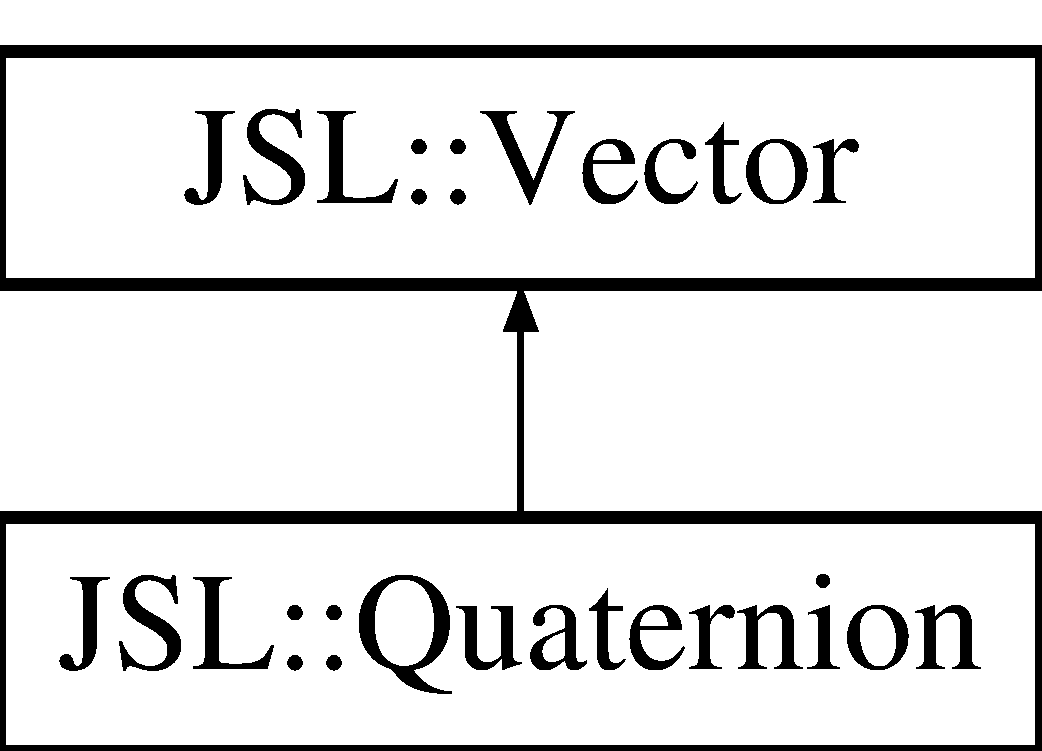
\includegraphics[height=2.000000cm]{classJSL_1_1Quaternion}
\end{center}
\end{figure}
\doxysubsection*{Public Member Functions}
\begin{DoxyCompactItemize}
\item 
\mbox{\hyperlink{classJSL_1_1Quaternion_a3bfe577832b38cdf2dbbb143c9487add}{Quaternion}} ()
\item 
\mbox{\hyperlink{classJSL_1_1Quaternion_ae31be96e94176f1e5278cfaeba39dedc}{Quaternion}} (const double \&scalar, const \mbox{\hyperlink{classJSL_1_1Vector}{J\+S\+L\+::\+Vector}} \&vec)
\item 
\mbox{\hyperlink{classJSL_1_1Quaternion_ac0fa428adfcbc3db2eff9b5c86e7a075}{Quaternion}} (const double \&a, const double \&b, const double \&c, const double \&d)
\item 
\mbox{\hyperlink{classJSL_1_1Quaternion_a6b71605f5fafada8e94bab1bf9af55bd}{Quaternion}} (const \mbox{\hyperlink{classJSL_1_1Vector}{J\+S\+L\+::\+Vector}} \&vec4)
\item 
\mbox{\hyperlink{classJSL_1_1Quaternion_a738b4fb82caf2a0334818ac4e6c494de}{Quaternion}} (const std\+::vector$<$ double $>$ \&vec4)
\item 
double \& \mbox{\hyperlink{classJSL_1_1Quaternion_a67d6b60a4863985f94d23c68953dcd91}{Scalar}} ()
\item 
double \& \mbox{\hyperlink{classJSL_1_1Quaternion_a92b7311aecae986edb373e0b40d5bfdd}{Vector}} (int id)
\item 
const double \& \mbox{\hyperlink{classJSL_1_1Quaternion_aba8a8ac1d2101f8b374387349412035b}{Scalar}} () const
\item 
const double \& \mbox{\hyperlink{classJSL_1_1Quaternion_a5243fa5db9d466bf1485a83325a682b0}{Vector}} (int id) const
\item 
\mbox{\hyperlink{classJSL_1_1Vector}{J\+S\+L\+::\+Vector}} \mbox{\hyperlink{classJSL_1_1Quaternion_a0255f2026ec4af9cff42d09d2309af01}{Vector}} () const
\item 
\mbox{\hyperlink{classJSL_1_1Quaternion}{Quaternion}} \mbox{\hyperlink{classJSL_1_1Quaternion_a9bea717f4cd1b5d4e3bdb8eedfbaed2c}{Conjugate}} () const
\item 
\mbox{\hyperlink{classJSL_1_1Matrix}{J\+S\+L\+::\+Matrix}} \mbox{\hyperlink{classJSL_1_1Quaternion_ada6a7067e13b60a65a6103f7508f62f3}{Left\+Multiplication\+Matrix}} () const
\item 
\mbox{\hyperlink{classJSL_1_1Matrix}{J\+S\+L\+::\+Matrix}} \mbox{\hyperlink{classJSL_1_1Quaternion_a081b38fc741f2dc9d4f2b955acbed833}{Right\+Multiplication\+Matrix}} () const
\end{DoxyCompactItemize}
\doxysubsection*{Static Public Member Functions}
\begin{DoxyCompactItemize}
\item 
static \mbox{\hyperlink{classJSL_1_1Quaternion}{Quaternion}} \mbox{\hyperlink{classJSL_1_1Quaternion_adf0c22bf67a2ab873b998b34583de2e0}{One}} ()
\item 
static \mbox{\hyperlink{classJSL_1_1Quaternion}{Quaternion}} \mbox{\hyperlink{classJSL_1_1Quaternion_a63e84edb5230efc8378d86b5d182221d}{Zero}} ()
\item 
static \mbox{\hyperlink{classJSL_1_1Quaternion}{Quaternion}} \mbox{\hyperlink{classJSL_1_1Quaternion_a8d47df19d5d74b82a8e348391e8ef8c4}{Random}} ()
\end{DoxyCompactItemize}
\doxysubsection*{Additional Inherited Members}


\doxysubsection{Constructor \& Destructor Documentation}
\mbox{\Hypertarget{classJSL_1_1Quaternion_a3bfe577832b38cdf2dbbb143c9487add}\label{classJSL_1_1Quaternion_a3bfe577832b38cdf2dbbb143c9487add}} 
\index{JSL::Quaternion@{JSL::Quaternion}!Quaternion@{Quaternion}}
\index{Quaternion@{Quaternion}!JSL::Quaternion@{JSL::Quaternion}}
\doxysubsubsection{\texorpdfstring{Quaternion()}{Quaternion()}\hspace{0.1cm}{\footnotesize\ttfamily [1/5]}}
{\footnotesize\ttfamily J\+S\+L\+::\+Quaternion\+::\+Quaternion (\begin{DoxyParamCaption}{ }\end{DoxyParamCaption})\hspace{0.3cm}{\ttfamily [inline]}}

\mbox{\Hypertarget{classJSL_1_1Quaternion_ae31be96e94176f1e5278cfaeba39dedc}\label{classJSL_1_1Quaternion_ae31be96e94176f1e5278cfaeba39dedc}} 
\index{JSL::Quaternion@{JSL::Quaternion}!Quaternion@{Quaternion}}
\index{Quaternion@{Quaternion}!JSL::Quaternion@{JSL::Quaternion}}
\doxysubsubsection{\texorpdfstring{Quaternion()}{Quaternion()}\hspace{0.1cm}{\footnotesize\ttfamily [2/5]}}
{\footnotesize\ttfamily J\+S\+L\+::\+Quaternion\+::\+Quaternion (\begin{DoxyParamCaption}\item[{const double \&}]{scalar,  }\item[{const \mbox{\hyperlink{classJSL_1_1Vector}{J\+S\+L\+::\+Vector}} \&}]{vec }\end{DoxyParamCaption})\hspace{0.3cm}{\ttfamily [inline]}}

\mbox{\Hypertarget{classJSL_1_1Quaternion_ac0fa428adfcbc3db2eff9b5c86e7a075}\label{classJSL_1_1Quaternion_ac0fa428adfcbc3db2eff9b5c86e7a075}} 
\index{JSL::Quaternion@{JSL::Quaternion}!Quaternion@{Quaternion}}
\index{Quaternion@{Quaternion}!JSL::Quaternion@{JSL::Quaternion}}
\doxysubsubsection{\texorpdfstring{Quaternion()}{Quaternion()}\hspace{0.1cm}{\footnotesize\ttfamily [3/5]}}
{\footnotesize\ttfamily J\+S\+L\+::\+Quaternion\+::\+Quaternion (\begin{DoxyParamCaption}\item[{const double \&}]{a,  }\item[{const double \&}]{b,  }\item[{const double \&}]{c,  }\item[{const double \&}]{d }\end{DoxyParamCaption})\hspace{0.3cm}{\ttfamily [inline]}}

\mbox{\Hypertarget{classJSL_1_1Quaternion_a6b71605f5fafada8e94bab1bf9af55bd}\label{classJSL_1_1Quaternion_a6b71605f5fafada8e94bab1bf9af55bd}} 
\index{JSL::Quaternion@{JSL::Quaternion}!Quaternion@{Quaternion}}
\index{Quaternion@{Quaternion}!JSL::Quaternion@{JSL::Quaternion}}
\doxysubsubsection{\texorpdfstring{Quaternion()}{Quaternion()}\hspace{0.1cm}{\footnotesize\ttfamily [4/5]}}
{\footnotesize\ttfamily J\+S\+L\+::\+Quaternion\+::\+Quaternion (\begin{DoxyParamCaption}\item[{const \mbox{\hyperlink{classJSL_1_1Vector}{J\+S\+L\+::\+Vector}} \&}]{vec4 }\end{DoxyParamCaption})\hspace{0.3cm}{\ttfamily [inline]}}

\mbox{\Hypertarget{classJSL_1_1Quaternion_a738b4fb82caf2a0334818ac4e6c494de}\label{classJSL_1_1Quaternion_a738b4fb82caf2a0334818ac4e6c494de}} 
\index{JSL::Quaternion@{JSL::Quaternion}!Quaternion@{Quaternion}}
\index{Quaternion@{Quaternion}!JSL::Quaternion@{JSL::Quaternion}}
\doxysubsubsection{\texorpdfstring{Quaternion()}{Quaternion()}\hspace{0.1cm}{\footnotesize\ttfamily [5/5]}}
{\footnotesize\ttfamily J\+S\+L\+::\+Quaternion\+::\+Quaternion (\begin{DoxyParamCaption}\item[{const std\+::vector$<$ double $>$ \&}]{vec4 }\end{DoxyParamCaption})\hspace{0.3cm}{\ttfamily [inline]}}



\doxysubsection{Member Function Documentation}
\mbox{\Hypertarget{classJSL_1_1Quaternion_a9bea717f4cd1b5d4e3bdb8eedfbaed2c}\label{classJSL_1_1Quaternion_a9bea717f4cd1b5d4e3bdb8eedfbaed2c}} 
\index{JSL::Quaternion@{JSL::Quaternion}!Conjugate@{Conjugate}}
\index{Conjugate@{Conjugate}!JSL::Quaternion@{JSL::Quaternion}}
\doxysubsubsection{\texorpdfstring{Conjugate()}{Conjugate()}}
{\footnotesize\ttfamily \mbox{\hyperlink{classJSL_1_1Quaternion}{Quaternion}} J\+S\+L\+::\+Quaternion\+::\+Conjugate (\begin{DoxyParamCaption}{ }\end{DoxyParamCaption}) const\hspace{0.3cm}{\ttfamily [inline]}}

\mbox{\Hypertarget{classJSL_1_1Quaternion_ada6a7067e13b60a65a6103f7508f62f3}\label{classJSL_1_1Quaternion_ada6a7067e13b60a65a6103f7508f62f3}} 
\index{JSL::Quaternion@{JSL::Quaternion}!LeftMultiplicationMatrix@{LeftMultiplicationMatrix}}
\index{LeftMultiplicationMatrix@{LeftMultiplicationMatrix}!JSL::Quaternion@{JSL::Quaternion}}
\doxysubsubsection{\texorpdfstring{LeftMultiplicationMatrix()}{LeftMultiplicationMatrix()}}
{\footnotesize\ttfamily \mbox{\hyperlink{classJSL_1_1Matrix}{J\+S\+L\+::\+Matrix}} J\+S\+L\+::\+Quaternion\+::\+Left\+Multiplication\+Matrix (\begin{DoxyParamCaption}{ }\end{DoxyParamCaption}) const\hspace{0.3cm}{\ttfamily [inline]}}

\mbox{\Hypertarget{classJSL_1_1Quaternion_adf0c22bf67a2ab873b998b34583de2e0}\label{classJSL_1_1Quaternion_adf0c22bf67a2ab873b998b34583de2e0}} 
\index{JSL::Quaternion@{JSL::Quaternion}!One@{One}}
\index{One@{One}!JSL::Quaternion@{JSL::Quaternion}}
\doxysubsubsection{\texorpdfstring{One()}{One()}}
{\footnotesize\ttfamily static \mbox{\hyperlink{classJSL_1_1Quaternion}{Quaternion}} J\+S\+L\+::\+Quaternion\+::\+One (\begin{DoxyParamCaption}{ }\end{DoxyParamCaption})\hspace{0.3cm}{\ttfamily [inline]}, {\ttfamily [static]}}

\mbox{\Hypertarget{classJSL_1_1Quaternion_a8d47df19d5d74b82a8e348391e8ef8c4}\label{classJSL_1_1Quaternion_a8d47df19d5d74b82a8e348391e8ef8c4}} 
\index{JSL::Quaternion@{JSL::Quaternion}!Random@{Random}}
\index{Random@{Random}!JSL::Quaternion@{JSL::Quaternion}}
\doxysubsubsection{\texorpdfstring{Random()}{Random()}}
{\footnotesize\ttfamily static \mbox{\hyperlink{classJSL_1_1Quaternion}{Quaternion}} J\+S\+L\+::\+Quaternion\+::\+Random (\begin{DoxyParamCaption}{ }\end{DoxyParamCaption})\hspace{0.3cm}{\ttfamily [inline]}, {\ttfamily [static]}}

\mbox{\Hypertarget{classJSL_1_1Quaternion_a081b38fc741f2dc9d4f2b955acbed833}\label{classJSL_1_1Quaternion_a081b38fc741f2dc9d4f2b955acbed833}} 
\index{JSL::Quaternion@{JSL::Quaternion}!RightMultiplicationMatrix@{RightMultiplicationMatrix}}
\index{RightMultiplicationMatrix@{RightMultiplicationMatrix}!JSL::Quaternion@{JSL::Quaternion}}
\doxysubsubsection{\texorpdfstring{RightMultiplicationMatrix()}{RightMultiplicationMatrix()}}
{\footnotesize\ttfamily \mbox{\hyperlink{classJSL_1_1Matrix}{J\+S\+L\+::\+Matrix}} J\+S\+L\+::\+Quaternion\+::\+Right\+Multiplication\+Matrix (\begin{DoxyParamCaption}{ }\end{DoxyParamCaption}) const\hspace{0.3cm}{\ttfamily [inline]}}

\mbox{\Hypertarget{classJSL_1_1Quaternion_a67d6b60a4863985f94d23c68953dcd91}\label{classJSL_1_1Quaternion_a67d6b60a4863985f94d23c68953dcd91}} 
\index{JSL::Quaternion@{JSL::Quaternion}!Scalar@{Scalar}}
\index{Scalar@{Scalar}!JSL::Quaternion@{JSL::Quaternion}}
\doxysubsubsection{\texorpdfstring{Scalar()}{Scalar()}\hspace{0.1cm}{\footnotesize\ttfamily [1/2]}}
{\footnotesize\ttfamily double\& J\+S\+L\+::\+Quaternion\+::\+Scalar (\begin{DoxyParamCaption}{ }\end{DoxyParamCaption})\hspace{0.3cm}{\ttfamily [inline]}}

\mbox{\Hypertarget{classJSL_1_1Quaternion_aba8a8ac1d2101f8b374387349412035b}\label{classJSL_1_1Quaternion_aba8a8ac1d2101f8b374387349412035b}} 
\index{JSL::Quaternion@{JSL::Quaternion}!Scalar@{Scalar}}
\index{Scalar@{Scalar}!JSL::Quaternion@{JSL::Quaternion}}
\doxysubsubsection{\texorpdfstring{Scalar()}{Scalar()}\hspace{0.1cm}{\footnotesize\ttfamily [2/2]}}
{\footnotesize\ttfamily const double\& J\+S\+L\+::\+Quaternion\+::\+Scalar (\begin{DoxyParamCaption}{ }\end{DoxyParamCaption}) const\hspace{0.3cm}{\ttfamily [inline]}}

\mbox{\Hypertarget{classJSL_1_1Quaternion_a0255f2026ec4af9cff42d09d2309af01}\label{classJSL_1_1Quaternion_a0255f2026ec4af9cff42d09d2309af01}} 
\index{JSL::Quaternion@{JSL::Quaternion}!Vector@{Vector}}
\index{Vector@{Vector}!JSL::Quaternion@{JSL::Quaternion}}
\doxysubsubsection{\texorpdfstring{Vector()}{Vector()}\hspace{0.1cm}{\footnotesize\ttfamily [1/3]}}
{\footnotesize\ttfamily \mbox{\hyperlink{classJSL_1_1Vector}{J\+S\+L\+::\+Vector}} J\+S\+L\+::\+Quaternion\+::\+Vector (\begin{DoxyParamCaption}{ }\end{DoxyParamCaption}) const\hspace{0.3cm}{\ttfamily [inline]}}

\mbox{\Hypertarget{classJSL_1_1Quaternion_a92b7311aecae986edb373e0b40d5bfdd}\label{classJSL_1_1Quaternion_a92b7311aecae986edb373e0b40d5bfdd}} 
\index{JSL::Quaternion@{JSL::Quaternion}!Vector@{Vector}}
\index{Vector@{Vector}!JSL::Quaternion@{JSL::Quaternion}}
\doxysubsubsection{\texorpdfstring{Vector()}{Vector()}\hspace{0.1cm}{\footnotesize\ttfamily [2/3]}}
{\footnotesize\ttfamily double\& J\+S\+L\+::\+Quaternion\+::\+Vector (\begin{DoxyParamCaption}\item[{int}]{id }\end{DoxyParamCaption})\hspace{0.3cm}{\ttfamily [inline]}}

\mbox{\Hypertarget{classJSL_1_1Quaternion_a5243fa5db9d466bf1485a83325a682b0}\label{classJSL_1_1Quaternion_a5243fa5db9d466bf1485a83325a682b0}} 
\index{JSL::Quaternion@{JSL::Quaternion}!Vector@{Vector}}
\index{Vector@{Vector}!JSL::Quaternion@{JSL::Quaternion}}
\doxysubsubsection{\texorpdfstring{Vector()}{Vector()}\hspace{0.1cm}{\footnotesize\ttfamily [3/3]}}
{\footnotesize\ttfamily const double\& J\+S\+L\+::\+Quaternion\+::\+Vector (\begin{DoxyParamCaption}\item[{int}]{id }\end{DoxyParamCaption}) const\hspace{0.3cm}{\ttfamily [inline]}}

\mbox{\Hypertarget{classJSL_1_1Quaternion_a63e84edb5230efc8378d86b5d182221d}\label{classJSL_1_1Quaternion_a63e84edb5230efc8378d86b5d182221d}} 
\index{JSL::Quaternion@{JSL::Quaternion}!Zero@{Zero}}
\index{Zero@{Zero}!JSL::Quaternion@{JSL::Quaternion}}
\doxysubsubsection{\texorpdfstring{Zero()}{Zero()}}
{\footnotesize\ttfamily static \mbox{\hyperlink{classJSL_1_1Quaternion}{Quaternion}} J\+S\+L\+::\+Quaternion\+::\+Zero (\begin{DoxyParamCaption}{ }\end{DoxyParamCaption})\hspace{0.3cm}{\ttfamily [inline]}, {\ttfamily [static]}}



The documentation for this class was generated from the following file\+:\begin{DoxyCompactItemize}
\item 
/home/jack/\+Documents/\+Work/\+Q\+Dynamics/lib/\+J\+S\+L/\+Maths/\mbox{\hyperlink{Q__temp_8h}{Q\+\_\+temp.\+h}}\end{DoxyCompactItemize}

\hypertarget{classJSL__Testing_1_1StringTest}{}\section{J\+S\+L\+\_\+\+Testing\+:\+:String\+Test Class Reference}
\label{classJSL__Testing_1_1StringTest}\index{J\+S\+L\+\_\+\+Testing\+::\+String\+Test@{J\+S\+L\+\_\+\+Testing\+::\+String\+Test}}


{\ttfamily \#include $<$Testing\+\_\+\+Unit\+Tests.\+h$>$}

Inheritance diagram for J\+S\+L\+\_\+\+Testing\+:\+:String\+Test\+:\begin{figure}[H]
\begin{center}
\leavevmode
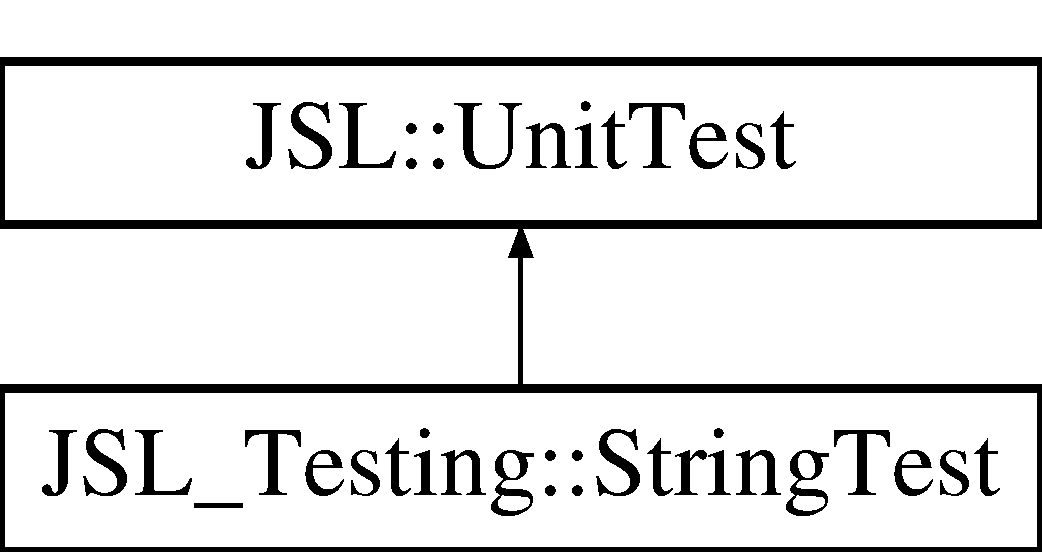
\includegraphics[height=2.000000cm]{classJSL__Testing_1_1StringTest}
\end{center}
\end{figure}
\subsection*{Public Member Functions}
\begin{DoxyCompactItemize}
\item 
\hyperlink{classJSL__Testing_1_1StringTest_a5be5ef071697a4e106c1a1e51ded1cf6}{String\+Test} ()
\item 
void \hyperlink{classJSL__Testing_1_1StringTest_ada0409cd10e3f09788994a9115331ff7}{Run\+\_\+\+Test} ()
\begin{DoxyCompactList}\small\item\em All children which want to take advantage of the \hyperlink{classJSL_1_1UnitTest_aabec19b081be8a428f12e4b5e3dc2a9c}{Buffered\+Test()} command should have the bulk of their testing within this command. \end{DoxyCompactList}\end{DoxyCompactItemize}
\subsection*{Additional Inherited Members}


\subsection{Constructor \& Destructor Documentation}
\mbox{\Hypertarget{classJSL__Testing_1_1StringTest_a5be5ef071697a4e106c1a1e51ded1cf6}\label{classJSL__Testing_1_1StringTest_a5be5ef071697a4e106c1a1e51ded1cf6}} 
\index{J\+S\+L\+\_\+\+Testing\+::\+String\+Test@{J\+S\+L\+\_\+\+Testing\+::\+String\+Test}!String\+Test@{String\+Test}}
\index{String\+Test@{String\+Test}!J\+S\+L\+\_\+\+Testing\+::\+String\+Test@{J\+S\+L\+\_\+\+Testing\+::\+String\+Test}}
\subsubsection{\texorpdfstring{String\+Test()}{StringTest()}}
{\footnotesize\ttfamily J\+S\+L\+\_\+\+Testing\+::\+String\+Test\+::\+String\+Test (\begin{DoxyParamCaption}{ }\end{DoxyParamCaption})\hspace{0.3cm}{\ttfamily [inline]}}



\subsection{Member Function Documentation}
\mbox{\Hypertarget{classJSL__Testing_1_1StringTest_ada0409cd10e3f09788994a9115331ff7}\label{classJSL__Testing_1_1StringTest_ada0409cd10e3f09788994a9115331ff7}} 
\index{J\+S\+L\+\_\+\+Testing\+::\+String\+Test@{J\+S\+L\+\_\+\+Testing\+::\+String\+Test}!Run\+\_\+\+Test@{Run\+\_\+\+Test}}
\index{Run\+\_\+\+Test@{Run\+\_\+\+Test}!J\+S\+L\+\_\+\+Testing\+::\+String\+Test@{J\+S\+L\+\_\+\+Testing\+::\+String\+Test}}
\subsubsection{\texorpdfstring{Run\+\_\+\+Test()}{Run\_Test()}}
{\footnotesize\ttfamily void J\+S\+L\+\_\+\+Testing\+::\+String\+Test\+::\+Run\+\_\+\+Test (\begin{DoxyParamCaption}{ }\end{DoxyParamCaption})\hspace{0.3cm}{\ttfamily [inline]}, {\ttfamily [virtual]}}



All children which want to take advantage of the \hyperlink{classJSL_1_1UnitTest_aabec19b081be8a428f12e4b5e3dc2a9c}{Buffered\+Test()} command should have the bulk of their testing within this command. 



Reimplemented from \hyperlink{classJSL_1_1UnitTest_aa8369ab1ce2a537bff2ea7e1c8818490}{J\+S\+L\+::\+Unit\+Test}.



The documentation for this class was generated from the following file\+:\begin{DoxyCompactItemize}
\item 
/home/f/fraserj/\+Documents/\+Work/\+Q\+Dynamics/lib/\+J\+S\+L/\+Testing/\hyperlink{Testing__UnitTests_8h}{Testing\+\_\+\+Unit\+Tests.\+h}\end{DoxyCompactItemize}

\hypertarget{classQDynamics_1_1Symi}{}\section{Q\+Dynamics\+:\+:Symi Class Reference}
\label{classQDynamics_1_1Symi}\index{Q\+Dynamics\+::\+Symi@{Q\+Dynamics\+::\+Symi}}


{\ttfamily \#include $<$Symi.\+h$>$}

Inheritance diagram for Q\+Dynamics\+:\+:Symi\+:\begin{figure}[H]
\begin{center}
\leavevmode
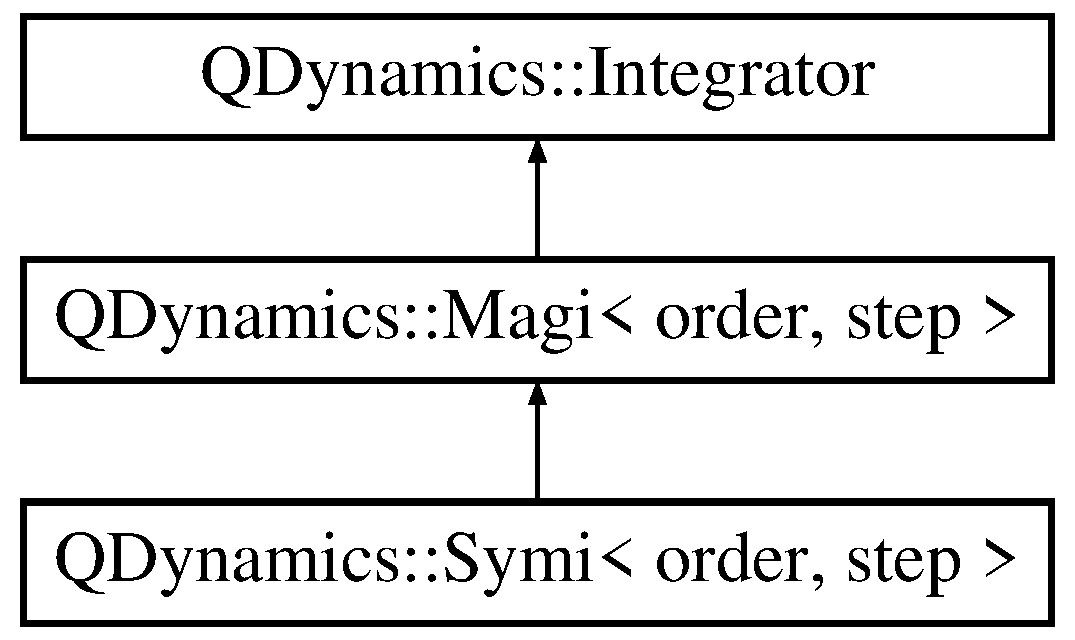
\includegraphics[height=4.000000cm]{classQDynamics_1_1Symi}
\end{center}
\end{figure}
\subsection*{Public Member Functions}
\begin{DoxyCompactItemize}
\item 
\hyperlink{classQDynamics_1_1Symi_afc73292268197d37fad6716aa6bb5976}{Symi} (int order, double T, double deltaT)
\item 
\hyperlink{classQDynamics_1_1Symi_a2e248bf5141814ca1e8285227d26d4bc}{Symi} (int order, double T, double deltaT, int skipper)
\end{DoxyCompactItemize}
\subsection*{Protected Member Functions}
\begin{DoxyCompactItemize}
\item 
virtual \hyperlink{classQDynamics_1_1Quaternion}{Quaternion} \hyperlink{classQDynamics_1_1Symi_a4cea691ad899227f92004dd666180415}{Magnus\+\_\+\+Compute} (double duration)
\end{DoxyCompactItemize}
\subsection*{Additional Inherited Members}


\subsection{Constructor \& Destructor Documentation}
\mbox{\Hypertarget{classQDynamics_1_1Symi_afc73292268197d37fad6716aa6bb5976}\label{classQDynamics_1_1Symi_afc73292268197d37fad6716aa6bb5976}} 
\index{Q\+Dynamics\+::\+Symi@{Q\+Dynamics\+::\+Symi}!Symi@{Symi}}
\index{Symi@{Symi}!Q\+Dynamics\+::\+Symi@{Q\+Dynamics\+::\+Symi}}
\subsubsection{\texorpdfstring{Symi()}{Symi()}\hspace{0.1cm}{\footnotesize\ttfamily [1/2]}}
{\footnotesize\ttfamily Q\+Dynamics\+::\+Symi\+::\+Symi (\begin{DoxyParamCaption}\item[{int}]{order,  }\item[{double}]{T,  }\item[{double}]{deltaT }\end{DoxyParamCaption})\hspace{0.3cm}{\ttfamily [inline]}}

\mbox{\Hypertarget{classQDynamics_1_1Symi_a2e248bf5141814ca1e8285227d26d4bc}\label{classQDynamics_1_1Symi_a2e248bf5141814ca1e8285227d26d4bc}} 
\index{Q\+Dynamics\+::\+Symi@{Q\+Dynamics\+::\+Symi}!Symi@{Symi}}
\index{Symi@{Symi}!Q\+Dynamics\+::\+Symi@{Q\+Dynamics\+::\+Symi}}
\subsubsection{\texorpdfstring{Symi()}{Symi()}\hspace{0.1cm}{\footnotesize\ttfamily [2/2]}}
{\footnotesize\ttfamily Q\+Dynamics\+::\+Symi\+::\+Symi (\begin{DoxyParamCaption}\item[{int}]{order,  }\item[{double}]{T,  }\item[{double}]{deltaT,  }\item[{int}]{skipper }\end{DoxyParamCaption})\hspace{0.3cm}{\ttfamily [inline]}}



\subsection{Member Function Documentation}
\mbox{\Hypertarget{classQDynamics_1_1Symi_a4cea691ad899227f92004dd666180415}\label{classQDynamics_1_1Symi_a4cea691ad899227f92004dd666180415}} 
\index{Q\+Dynamics\+::\+Symi@{Q\+Dynamics\+::\+Symi}!Magnus\+\_\+\+Compute@{Magnus\+\_\+\+Compute}}
\index{Magnus\+\_\+\+Compute@{Magnus\+\_\+\+Compute}!Q\+Dynamics\+::\+Symi@{Q\+Dynamics\+::\+Symi}}
\subsubsection{\texorpdfstring{Magnus\+\_\+\+Compute()}{Magnus\_Compute()}}
{\footnotesize\ttfamily virtual \hyperlink{classQDynamics_1_1Quaternion}{Quaternion} Q\+Dynamics\+::\+Symi\+::\+Magnus\+\_\+\+Compute (\begin{DoxyParamCaption}\item[{double}]{duration }\end{DoxyParamCaption})\hspace{0.3cm}{\ttfamily [inline]}, {\ttfamily [protected]}, {\ttfamily [virtual]}}



Reimplemented from \hyperlink{classQDynamics_1_1Magi_aadacdb3581a42babd5e1aa9ada6c77ee}{Q\+Dynamics\+::\+Magi}.



The documentation for this class was generated from the following file\+:\begin{DoxyCompactItemize}
\item 
/home/f/fraserj/\+Documents/\+Work/\+Q\+Dynamics/src/\hyperlink{Symi_8h}{Symi.\+h}\end{DoxyCompactItemize}

\hypertarget{classQDynamics_1_1SymiL}{}\doxysection{Q\+Dynamics\+::SymiL Class Reference}
\label{classQDynamics_1_1SymiL}\index{QDynamics::SymiL@{QDynamics::SymiL}}


{\ttfamily \#include $<$Symi.\+h$>$}

Inheritance diagram for Q\+Dynamics\+::SymiL\+:\begin{figure}[H]
\begin{center}
\leavevmode
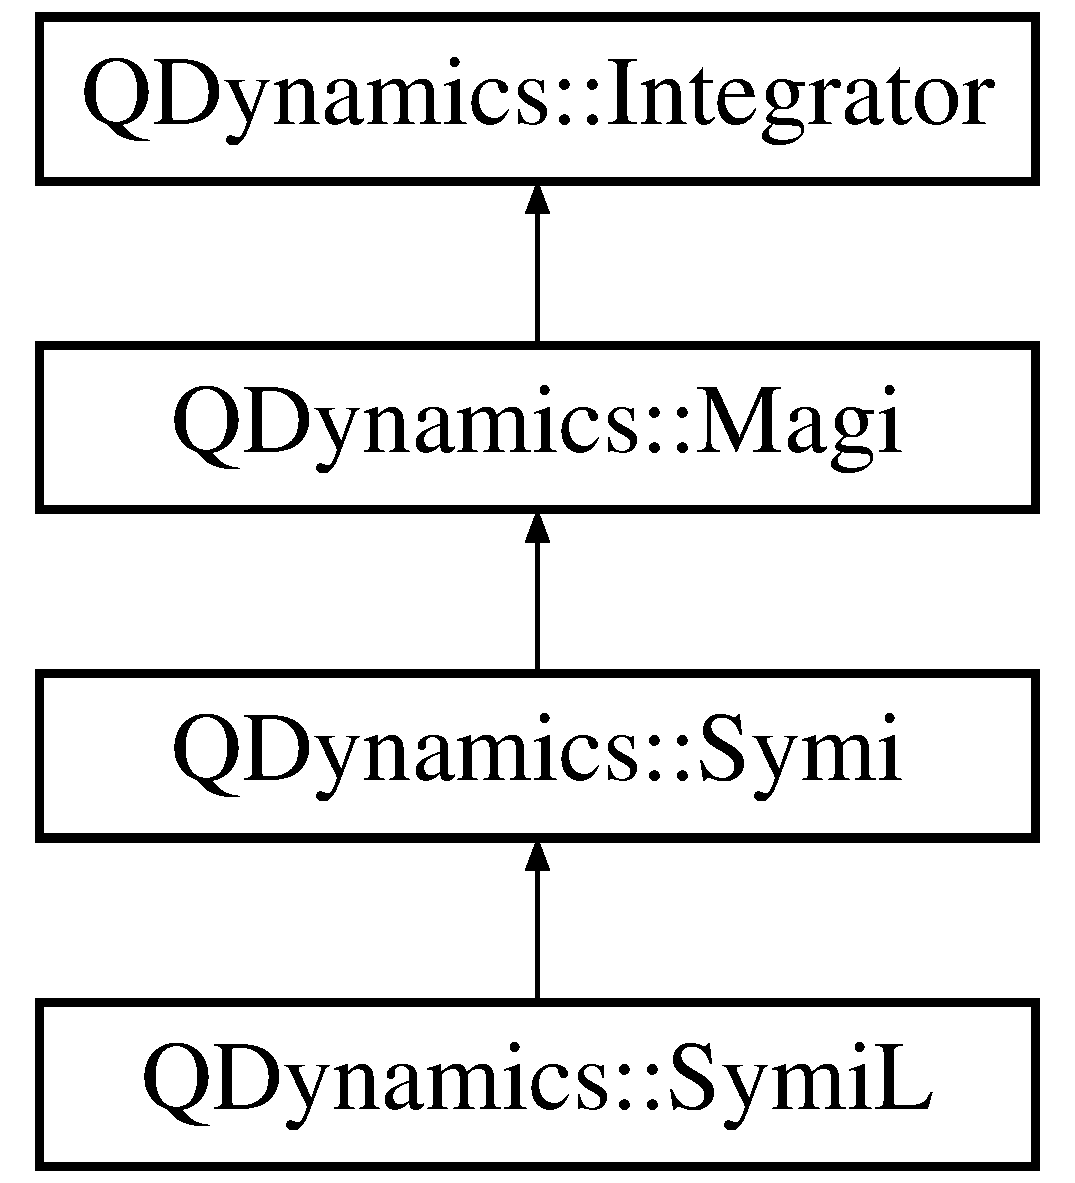
\includegraphics[height=4.000000cm]{classQDynamics_1_1SymiL}
\end{center}
\end{figure}
\doxysubsection*{Public Member Functions}
\begin{DoxyCompactItemize}
\item 
\mbox{\hyperlink{classQDynamics_1_1SymiL_ac220b2a8cccf6c3c8ca0d0f79c094fe7}{SymiL}} (int order, double T, double deltaT)
\item 
\mbox{\hyperlink{classQDynamics_1_1SymiL_acdb13fb6bc527f687385dbdb05ff6e17}{SymiL}} (int order, double T, double deltaT, int skipper)
\end{DoxyCompactItemize}
\doxysubsection*{Private Member Functions}
\begin{DoxyCompactItemize}
\item 
virtual void \mbox{\hyperlink{classQDynamics_1_1SymiL_a28d23793abeb8f40c9d9ec069d67debb}{Update\+Position}} (double t)
\begin{DoxyCompactList}\small\item\em In the \mbox{\hyperlink{classQDynamics_1_1Integrator}{Integrator}} base class, this is an empty function. Child members will mainly focus on overloading this function to their own update formula. \end{DoxyCompactList}\end{DoxyCompactItemize}
\doxysubsection*{Additional Inherited Members}


\doxysubsection{Constructor \& Destructor Documentation}
\mbox{\Hypertarget{classQDynamics_1_1SymiL_ac220b2a8cccf6c3c8ca0d0f79c094fe7}\label{classQDynamics_1_1SymiL_ac220b2a8cccf6c3c8ca0d0f79c094fe7}} 
\index{QDynamics::SymiL@{QDynamics::SymiL}!SymiL@{SymiL}}
\index{SymiL@{SymiL}!QDynamics::SymiL@{QDynamics::SymiL}}
\doxysubsubsection{\texorpdfstring{SymiL()}{SymiL()}\hspace{0.1cm}{\footnotesize\ttfamily [1/2]}}
{\footnotesize\ttfamily Q\+Dynamics\+::\+Symi\+L\+::\+SymiL (\begin{DoxyParamCaption}\item[{int}]{order,  }\item[{double}]{T,  }\item[{double}]{deltaT }\end{DoxyParamCaption})\hspace{0.3cm}{\ttfamily [inline]}}

\mbox{\Hypertarget{classQDynamics_1_1SymiL_acdb13fb6bc527f687385dbdb05ff6e17}\label{classQDynamics_1_1SymiL_acdb13fb6bc527f687385dbdb05ff6e17}} 
\index{QDynamics::SymiL@{QDynamics::SymiL}!SymiL@{SymiL}}
\index{SymiL@{SymiL}!QDynamics::SymiL@{QDynamics::SymiL}}
\doxysubsubsection{\texorpdfstring{SymiL()}{SymiL()}\hspace{0.1cm}{\footnotesize\ttfamily [2/2]}}
{\footnotesize\ttfamily Q\+Dynamics\+::\+Symi\+L\+::\+SymiL (\begin{DoxyParamCaption}\item[{int}]{order,  }\item[{double}]{T,  }\item[{double}]{deltaT,  }\item[{int}]{skipper }\end{DoxyParamCaption})\hspace{0.3cm}{\ttfamily [inline]}}



\doxysubsection{Member Function Documentation}
\mbox{\Hypertarget{classQDynamics_1_1SymiL_a28d23793abeb8f40c9d9ec069d67debb}\label{classQDynamics_1_1SymiL_a28d23793abeb8f40c9d9ec069d67debb}} 
\index{QDynamics::SymiL@{QDynamics::SymiL}!UpdatePosition@{UpdatePosition}}
\index{UpdatePosition@{UpdatePosition}!QDynamics::SymiL@{QDynamics::SymiL}}
\doxysubsubsection{\texorpdfstring{UpdatePosition()}{UpdatePosition()}}
{\footnotesize\ttfamily virtual void Q\+Dynamics\+::\+Symi\+L\+::\+Update\+Position (\begin{DoxyParamCaption}\item[{double}]{t }\end{DoxyParamCaption})\hspace{0.3cm}{\ttfamily [inline]}, {\ttfamily [private]}, {\ttfamily [virtual]}}



In the \mbox{\hyperlink{classQDynamics_1_1Integrator}{Integrator}} base class, this is an empty function. Child members will mainly focus on overloading this function to their own update formula. 


\begin{DoxyParams}{Parameters}
{\em t} & The current time of the integrator \\
\hline
\end{DoxyParams}


Reimplemented from \mbox{\hyperlink{classQDynamics_1_1Magi_a500467f899244edfae15f34c84c7684c}{Q\+Dynamics\+::\+Magi}}.



The documentation for this class was generated from the following file\+:\begin{DoxyCompactItemize}
\item 
/home/jack/\+Documents/\+Work/\+Q\+Dynamics/src/\mbox{\hyperlink{Symi_8h}{Symi.\+h}}\end{DoxyCompactItemize}

\hypertarget{classJSL_1_1UnitTest}{}\section{J\+SL\+:\+:Unit\+Test Class Reference}
\label{classJSL_1_1UnitTest}\index{J\+S\+L\+::\+Unit\+Test@{J\+S\+L\+::\+Unit\+Test}}


{\ttfamily \#include $<$Unit\+Test.\+h$>$}

Inheritance diagram for J\+SL\+:\+:Unit\+Test\+:\begin{figure}[H]
\begin{center}
\leavevmode
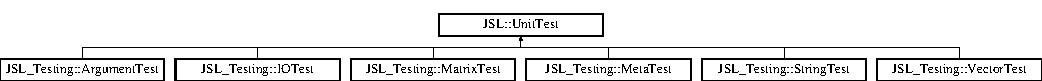
\includegraphics[height=1.085271cm]{classJSL_1_1UnitTest}
\end{center}
\end{figure}
\subsection*{Public Member Functions}
\begin{DoxyCompactItemize}
\item 
\hyperlink{classJSL_1_1UnitTest_aa3bc8d5c99696d5bc6e63b8da358a0ed}{Unit\+Test} ()
\begin{DoxyCompactList}\small\item\em Constructor class. Initialises the system to a failing state. \end{DoxyCompactList}\item 
virtual void \hyperlink{classJSL_1_1UnitTest_aa8369ab1ce2a537bff2ea7e1c8818490}{Run\+\_\+\+Test} ()
\begin{DoxyCompactList}\small\item\em All children which want to take advantage of the \hyperlink{classJSL_1_1UnitTest_aabec19b081be8a428f12e4b5e3dc2a9c}{Buffered\+Test()} command should have the bulk of their testing within this command. \end{DoxyCompactList}\item 
void \hyperlink{classJSL_1_1UnitTest_aabec19b081be8a428f12e4b5e3dc2a9c}{Buffered\+Test} ()
\begin{DoxyCompactList}\small\item\em Calls the overridden function \hyperlink{classJSL_1_1UnitTest_aa8369ab1ce2a537bff2ea7e1c8818490}{Run\+\_\+\+Test()} within a try-\/catch loop. Provides an extra level of safety and diagnostics for any unhandled exceptions. \end{DoxyCompactList}\item 
bool \hyperlink{classJSL_1_1UnitTest_a39e1076dd985334ce21606ae2a383f70}{Results} ()
\begin{DoxyCompactList}\small\item\em Prints the results of the testing to the terminal and prints the contents of Message\+Buffer line-\/by-\/line. \end{DoxyCompactList}\end{DoxyCompactItemize}
\subsection*{Data Fields}
\begin{DoxyCompactItemize}
\item 
std\+::string \hyperlink{classJSL_1_1UnitTest_a53c19424147e72fa6392470627f15049}{Name}
\begin{DoxyCompactList}\small\item\em The name by which the \hyperlink{classJSL_1_1UnitTest}{Unit\+Test} refers to itself. This should be fairly descriptive, to help locating the failing unit test (don\textquotesingle{}t give them all the same name!) \end{DoxyCompactList}\item 
bool \hyperlink{classJSL_1_1UnitTest_afac1f363a8406fad39316ee772a837a9}{Passed}
\begin{DoxyCompactList}\small\item\em If true, the \hyperlink{classJSL_1_1UnitTest}{Unit\+Test} is considered successful, and no errors are thrown. \end{DoxyCompactList}\item 
bool \hyperlink{classJSL_1_1UnitTest_a54dc4908d757c7f523be12a4275e595c}{Non\+Critical\+Failure}
\begin{DoxyCompactList}\small\item\em If true, the \hyperlink{classJSL_1_1UnitTest}{Unit\+Test} will only throw warnings, rather than exist, when an error is encountered. Default is false. \end{DoxyCompactList}\item 
std\+::vector$<$ std\+::string $>$ \hyperlink{classJSL_1_1UnitTest_a3dcc71e7e8f72f0f07b8fc552b777ad8}{Message\+Buffer}
\begin{DoxyCompactList}\small\item\em A message buffer which is output when \hyperlink{classJSL_1_1UnitTest_a39e1076dd985334ce21606ae2a383f70}{Results()} is called, giving updates on the progress of the test. \end{DoxyCompactList}\end{DoxyCompactItemize}
\subsection*{Protected Member Functions}
\begin{DoxyCompactItemize}
\item 
void \hyperlink{classJSL_1_1UnitTest_a3629d1bca071da7a2af6b7de29be1430}{basic\+Condition\+Check} (bool condition, std\+::string successmessage, std\+::string failuremessage)
\item 
void \hyperlink{classJSL_1_1UnitTest_a53ede0c6b420eaf64faf752c0518340e}{basic\+Condition\+Check} (bool condition, std\+::string message\+Framework)
\begin{DoxyCompactList}\small\item\em An override of the other function, preventing dual-\/typing of basic output messages. \end{DoxyCompactList}\end{DoxyCompactItemize}


\subsection{Detailed Description}
A parent class for various unit testing frameworks. Provides a consistent A\+PI for interacting with the unit tests. The class is essentially meaningless on its own, but when coupled to a decently written subclass (i.\+e. \hyperlink{classJSL__Testing_1_1StringTest}{J\+S\+L\+\_\+\+Testing\+::\+String\+Test}), it becomes very useful. 

\subsection{Constructor \& Destructor Documentation}
\mbox{\Hypertarget{classJSL_1_1UnitTest_aa3bc8d5c99696d5bc6e63b8da358a0ed}\label{classJSL_1_1UnitTest_aa3bc8d5c99696d5bc6e63b8da358a0ed}} 
\index{J\+S\+L\+::\+Unit\+Test@{J\+S\+L\+::\+Unit\+Test}!Unit\+Test@{Unit\+Test}}
\index{Unit\+Test@{Unit\+Test}!J\+S\+L\+::\+Unit\+Test@{J\+S\+L\+::\+Unit\+Test}}
\subsubsection{\texorpdfstring{Unit\+Test()}{UnitTest()}}
{\footnotesize\ttfamily J\+S\+L\+::\+Unit\+Test\+::\+Unit\+Test (\begin{DoxyParamCaption}{ }\end{DoxyParamCaption})\hspace{0.3cm}{\ttfamily [inline]}}



Constructor class. Initialises the system to a failing state. 



\subsection{Member Function Documentation}
\mbox{\Hypertarget{classJSL_1_1UnitTest_a3629d1bca071da7a2af6b7de29be1430}\label{classJSL_1_1UnitTest_a3629d1bca071da7a2af6b7de29be1430}} 
\index{J\+S\+L\+::\+Unit\+Test@{J\+S\+L\+::\+Unit\+Test}!basic\+Condition\+Check@{basic\+Condition\+Check}}
\index{basic\+Condition\+Check@{basic\+Condition\+Check}!J\+S\+L\+::\+Unit\+Test@{J\+S\+L\+::\+Unit\+Test}}
\subsubsection{\texorpdfstring{basic\+Condition\+Check()}{basicConditionCheck()}\hspace{0.1cm}{\footnotesize\ttfamily [1/2]}}
{\footnotesize\ttfamily void J\+S\+L\+::\+Unit\+Test\+::basic\+Condition\+Check (\begin{DoxyParamCaption}\item[{bool}]{condition,  }\item[{std\+::string}]{successmessage,  }\item[{std\+::string}]{failuremessage }\end{DoxyParamCaption})\hspace{0.3cm}{\ttfamily [inline]}, {\ttfamily [protected]}}

A structure to help basic logic flow within unit tests. If the condition is false, the unit test considers itself failed, and updates the messages and Passed status accordingly 
\begin{DoxyParams}{Parameters}
{\em condition} & If true, the sub-\/test is successful \\
\hline
{\em successmessage} & If condition == true, this is the message appended to the Message\+Buffer \\
\hline
{\em failuremessage} & If condition == false, this message is used instead. \\
\hline
\end{DoxyParams}
\mbox{\Hypertarget{classJSL_1_1UnitTest_a53ede0c6b420eaf64faf752c0518340e}\label{classJSL_1_1UnitTest_a53ede0c6b420eaf64faf752c0518340e}} 
\index{J\+S\+L\+::\+Unit\+Test@{J\+S\+L\+::\+Unit\+Test}!basic\+Condition\+Check@{basic\+Condition\+Check}}
\index{basic\+Condition\+Check@{basic\+Condition\+Check}!J\+S\+L\+::\+Unit\+Test@{J\+S\+L\+::\+Unit\+Test}}
\subsubsection{\texorpdfstring{basic\+Condition\+Check()}{basicConditionCheck()}\hspace{0.1cm}{\footnotesize\ttfamily [2/2]}}
{\footnotesize\ttfamily void J\+S\+L\+::\+Unit\+Test\+::basic\+Condition\+Check (\begin{DoxyParamCaption}\item[{bool}]{condition,  }\item[{std\+::string}]{message\+Framework }\end{DoxyParamCaption})\hspace{0.3cm}{\ttfamily [inline]}, {\ttfamily [protected]}}



An override of the other function, preventing dual-\/typing of basic output messages. 

\mbox{\Hypertarget{classJSL_1_1UnitTest_aabec19b081be8a428f12e4b5e3dc2a9c}\label{classJSL_1_1UnitTest_aabec19b081be8a428f12e4b5e3dc2a9c}} 
\index{J\+S\+L\+::\+Unit\+Test@{J\+S\+L\+::\+Unit\+Test}!Buffered\+Test@{Buffered\+Test}}
\index{Buffered\+Test@{Buffered\+Test}!J\+S\+L\+::\+Unit\+Test@{J\+S\+L\+::\+Unit\+Test}}
\subsubsection{\texorpdfstring{Buffered\+Test()}{BufferedTest()}}
{\footnotesize\ttfamily void J\+S\+L\+::\+Unit\+Test\+::\+Buffered\+Test (\begin{DoxyParamCaption}{ }\end{DoxyParamCaption})\hspace{0.3cm}{\ttfamily [inline]}}



Calls the overridden function \hyperlink{classJSL_1_1UnitTest_aa8369ab1ce2a537bff2ea7e1c8818490}{Run\+\_\+\+Test()} within a try-\/catch loop. Provides an extra level of safety and diagnostics for any unhandled exceptions. 

\mbox{\Hypertarget{classJSL_1_1UnitTest_a39e1076dd985334ce21606ae2a383f70}\label{classJSL_1_1UnitTest_a39e1076dd985334ce21606ae2a383f70}} 
\index{J\+S\+L\+::\+Unit\+Test@{J\+S\+L\+::\+Unit\+Test}!Results@{Results}}
\index{Results@{Results}!J\+S\+L\+::\+Unit\+Test@{J\+S\+L\+::\+Unit\+Test}}
\subsubsection{\texorpdfstring{Results()}{Results()}}
{\footnotesize\ttfamily bool J\+S\+L\+::\+Unit\+Test\+::\+Results (\begin{DoxyParamCaption}{ }\end{DoxyParamCaption})\hspace{0.3cm}{\ttfamily [inline]}}



Prints the results of the testing to the terminal and prints the contents of Message\+Buffer line-\/by-\/line. 

\begin{DoxyReturn}{Returns}
The value of Passed (true if test succeeded) 
\end{DoxyReturn}
\mbox{\Hypertarget{classJSL_1_1UnitTest_aa8369ab1ce2a537bff2ea7e1c8818490}\label{classJSL_1_1UnitTest_aa8369ab1ce2a537bff2ea7e1c8818490}} 
\index{J\+S\+L\+::\+Unit\+Test@{J\+S\+L\+::\+Unit\+Test}!Run\+\_\+\+Test@{Run\+\_\+\+Test}}
\index{Run\+\_\+\+Test@{Run\+\_\+\+Test}!J\+S\+L\+::\+Unit\+Test@{J\+S\+L\+::\+Unit\+Test}}
\subsubsection{\texorpdfstring{Run\+\_\+\+Test()}{Run\_Test()}}
{\footnotesize\ttfamily virtual void J\+S\+L\+::\+Unit\+Test\+::\+Run\+\_\+\+Test (\begin{DoxyParamCaption}{ }\end{DoxyParamCaption})\hspace{0.3cm}{\ttfamily [inline]}, {\ttfamily [virtual]}}



All children which want to take advantage of the \hyperlink{classJSL_1_1UnitTest_aabec19b081be8a428f12e4b5e3dc2a9c}{Buffered\+Test()} command should have the bulk of their testing within this command. 



Reimplemented in \hyperlink{classJSL__Testing_1_1MatrixTest_a8fe2a671faf414dbd13c407ab52b75fb}{J\+S\+L\+\_\+\+Testing\+::\+Matrix\+Test}, \hyperlink{classJSL__Testing_1_1VectorTest_ad79bb4654e6f7b59d31d7239ee0c2b82}{J\+S\+L\+\_\+\+Testing\+::\+Vector\+Test}, \hyperlink{classJSL__Testing_1_1ArgumentTest_a1c4c626d57e448da86866ef414308e97}{J\+S\+L\+\_\+\+Testing\+::\+Argument\+Test}, \hyperlink{classJSL__Testing_1_1IOTest_a85daecacc71354b5dc0dee36840b8704}{J\+S\+L\+\_\+\+Testing\+::\+I\+O\+Test}, \hyperlink{classJSL__Testing_1_1StringTest_ada0409cd10e3f09788994a9115331ff7}{J\+S\+L\+\_\+\+Testing\+::\+String\+Test}, and \hyperlink{classJSL__Testing_1_1MetaTest_a176352dcd54f9ec7df8f1548882e6820}{J\+S\+L\+\_\+\+Testing\+::\+Meta\+Test}.



\subsection{Field Documentation}
\mbox{\Hypertarget{classJSL_1_1UnitTest_a3dcc71e7e8f72f0f07b8fc552b777ad8}\label{classJSL_1_1UnitTest_a3dcc71e7e8f72f0f07b8fc552b777ad8}} 
\index{J\+S\+L\+::\+Unit\+Test@{J\+S\+L\+::\+Unit\+Test}!Message\+Buffer@{Message\+Buffer}}
\index{Message\+Buffer@{Message\+Buffer}!J\+S\+L\+::\+Unit\+Test@{J\+S\+L\+::\+Unit\+Test}}
\subsubsection{\texorpdfstring{Message\+Buffer}{MessageBuffer}}
{\footnotesize\ttfamily std\+::vector$<$std\+::string$>$ J\+S\+L\+::\+Unit\+Test\+::\+Message\+Buffer}



A message buffer which is output when \hyperlink{classJSL_1_1UnitTest_a39e1076dd985334ce21606ae2a383f70}{Results()} is called, giving updates on the progress of the test. 

\mbox{\Hypertarget{classJSL_1_1UnitTest_a53c19424147e72fa6392470627f15049}\label{classJSL_1_1UnitTest_a53c19424147e72fa6392470627f15049}} 
\index{J\+S\+L\+::\+Unit\+Test@{J\+S\+L\+::\+Unit\+Test}!Name@{Name}}
\index{Name@{Name}!J\+S\+L\+::\+Unit\+Test@{J\+S\+L\+::\+Unit\+Test}}
\subsubsection{\texorpdfstring{Name}{Name}}
{\footnotesize\ttfamily std\+::string J\+S\+L\+::\+Unit\+Test\+::\+Name}



The name by which the \hyperlink{classJSL_1_1UnitTest}{Unit\+Test} refers to itself. This should be fairly descriptive, to help locating the failing unit test (don\textquotesingle{}t give them all the same name!) 

\mbox{\Hypertarget{classJSL_1_1UnitTest_a54dc4908d757c7f523be12a4275e595c}\label{classJSL_1_1UnitTest_a54dc4908d757c7f523be12a4275e595c}} 
\index{J\+S\+L\+::\+Unit\+Test@{J\+S\+L\+::\+Unit\+Test}!Non\+Critical\+Failure@{Non\+Critical\+Failure}}
\index{Non\+Critical\+Failure@{Non\+Critical\+Failure}!J\+S\+L\+::\+Unit\+Test@{J\+S\+L\+::\+Unit\+Test}}
\subsubsection{\texorpdfstring{Non\+Critical\+Failure}{NonCriticalFailure}}
{\footnotesize\ttfamily bool J\+S\+L\+::\+Unit\+Test\+::\+Non\+Critical\+Failure}



If true, the \hyperlink{classJSL_1_1UnitTest}{Unit\+Test} will only throw warnings, rather than exist, when an error is encountered. Default is false. 

\mbox{\Hypertarget{classJSL_1_1UnitTest_afac1f363a8406fad39316ee772a837a9}\label{classJSL_1_1UnitTest_afac1f363a8406fad39316ee772a837a9}} 
\index{J\+S\+L\+::\+Unit\+Test@{J\+S\+L\+::\+Unit\+Test}!Passed@{Passed}}
\index{Passed@{Passed}!J\+S\+L\+::\+Unit\+Test@{J\+S\+L\+::\+Unit\+Test}}
\subsubsection{\texorpdfstring{Passed}{Passed}}
{\footnotesize\ttfamily bool J\+S\+L\+::\+Unit\+Test\+::\+Passed}



If true, the \hyperlink{classJSL_1_1UnitTest}{Unit\+Test} is considered successful, and no errors are thrown. 



The documentation for this class was generated from the following file\+:\begin{DoxyCompactItemize}
\item 
/home/f/fraserj/\+Documents/\+Work/\+Q\+Dynamics/lib/\+J\+S\+L/\+Testing/\hyperlink{UnitTest_8h}{Unit\+Test.\+h}\end{DoxyCompactItemize}

\hypertarget{classJSL_1_1Vector}{}\section{J\+SL\+:\+:Vector Class Reference}
\label{classJSL_1_1Vector}\index{J\+S\+L\+::\+Vector@{J\+S\+L\+::\+Vector}}


{\ttfamily \#include $<$vector.\+h$>$}

Inheritance diagram for J\+SL\+:\+:Vector\+:\begin{figure}[H]
\begin{center}
\leavevmode
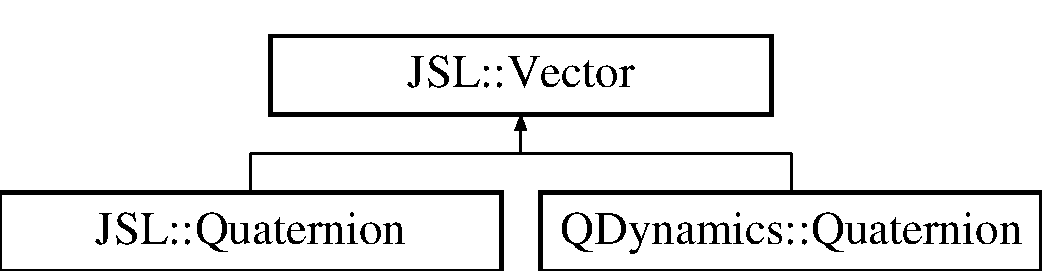
\includegraphics[height=2.000000cm]{classJSL_1_1Vector}
\end{center}
\end{figure}
\subsection*{Public Member Functions}
\begin{DoxyCompactItemize}
\item 
\hyperlink{classJSL_1_1Vector_a840fca607f8eae7dea1494b2954d3a3c}{Vector} ()
\item 
\hyperlink{classJSL_1_1Vector_aea8654ed3fb875d43f669a5f2e26fb25}{Vector} (int n)
\begin{DoxyCompactList}\small\item\em Initialises the vector to a state of length n, populated by zeros. \end{DoxyCompactList}\item 
\hyperlink{classJSL_1_1Vector_af5be93b29e1c2aab2882827d5001a2aa}{Vector} (std\+::vector$<$ double $>$ input)
\begin{DoxyCompactList}\small\item\em Initialises the vector to contain the provided stl vector. \end{DoxyCompactList}\item 
int \hyperlink{classJSL_1_1Vector_a53b26ca32061ebf41430fe2322f79c0c}{Size} () const
\item 
double \& \hyperlink{classJSL_1_1Vector_a7ff5112a7be30ca24b8ed953aaadd045}{operator\mbox{[}$\,$\mbox{]}} (int idx)
\begin{DoxyCompactList}\small\item\em Overload access operator so can call \hyperlink{classJSL_1_1Vector}{Vector}\mbox{[}0\mbox{]} etc as normal for a vector class. Performs checks on the size so that you cannot over/underflow the memory access. \end{DoxyCompactList}\item 
const double \& \hyperlink{classJSL_1_1Vector_ae461792ef0aeb62ac07c939dacedda99}{operator\mbox{[}$\,$\mbox{]}} (int idx) const
\begin{DoxyCompactList}\small\item\em Replication of non-\/const version (annoying) but necessary for good access.... \end{DoxyCompactList}\item 
double \hyperlink{classJSL_1_1Vector_a60660b5a26e0ddace46f31699834b671}{Dot} (const \hyperlink{classJSL_1_1Vector}{Vector} \&rhs) const
\begin{DoxyCompactList}\small\item\em Provides a member alias for \hyperlink{namespaceJSL_aeae64b7e0cfdc1ab5f35cca90c32d9f6}{Vector\+Dot\+Product()}, with the first argument being the current object. \end{DoxyCompactList}\item 
\hyperlink{classJSL_1_1Vector}{Vector} \hyperlink{classJSL_1_1Vector_a59ff98a99ebcf2b589290b9e57b8e184}{Cross} (const \hyperlink{classJSL_1_1Vector}{Vector} \&rhs) const
\begin{DoxyCompactList}\small\item\em Provides a member alias for \hyperlink{namespaceJSL_aa7816eb0cd81b74241ce460237990e70}{Vector\+Cross\+Product()}, with the first argument being the current object (recall order does matter for cross products!) \end{DoxyCompactList}\item 
double \hyperlink{classJSL_1_1Vector_ac1346e26bc981bf45d2c1c4317dac4e6}{Sq\+Norm} () const
\begin{DoxyCompactList}\small\item\em The squared-\/norm of the current object, calculated using \hyperlink{classJSL_1_1Vector_a60660b5a26e0ddace46f31699834b671}{Dot()}. Probably not as much use as \hyperlink{classJSL_1_1Vector_aa8af717591f5548ff471b6e4b28d7f9c}{Norm()}, but saves time sqrting and then squaring again! \end{DoxyCompactList}\item 
double \hyperlink{classJSL_1_1Vector_aa8af717591f5548ff471b6e4b28d7f9c}{Norm} () const
\begin{DoxyCompactList}\small\item\em The norm of the current object,. \end{DoxyCompactList}\item 
double \hyperlink{classJSL_1_1Vector_a0529640bc02ce994026184d93f43f9c3}{Angle\+Between} (const \hyperlink{classJSL_1_1Vector}{Vector} \&rhs) const
\begin{DoxyCompactList}\small\item\em A member-\/alias for \hyperlink{namespaceJSL_a09355c91f84fd99d4634bf9189fef51d}{Angle\+Between\+Vectors()}, with the first argument being the current object. \end{DoxyCompactList}\item 
std\+::string \hyperlink{classJSL_1_1Vector_a73579b4a194cc924341806a5d9ea3817}{to\+\_\+string} () const
\begin{DoxyCompactList}\small\item\em Converts the vector into a human-\/readable string. \end{DoxyCompactList}\item 
std\+::string \hyperlink{classJSL_1_1Vector_ad2d0bfdb432809a88a49f4576b0afb5a}{to\+\_\+simple\+\_\+string} () const
\item 
std\+::string \hyperlink{classJSL_1_1Vector_a91d4cf29c2865069520d03292844d84f}{to\+\_\+string\+\_\+precision} (const int n) const
\item 
\hyperlink{classJSL_1_1Vector}{Vector} \& \hyperlink{classJSL_1_1Vector_ad46bf395dd6122ce152c33aad2672a9b}{operator+=} (const \hyperlink{classJSL_1_1Vector}{Vector} \&rhs)
\begin{DoxyCompactList}\small\item\em In-\/place addition of two vectors. Calls \hyperlink{classJSL_1_1Vector}{Vector} \hyperlink{namespaceJSL_ae6530b77174d0dfae8e0d6e2a810f672}{operator+(const Vector \& lhs, const Vector \& rhs)} using this object as lhs. \end{DoxyCompactList}\item 
\hyperlink{classJSL_1_1Vector}{Vector} \& \hyperlink{classJSL_1_1Vector_a71720a9266944049cd3adfbe50e1703f}{operator-\/=} (const \hyperlink{classJSL_1_1Vector}{Vector} \&rhs)
\begin{DoxyCompactList}\small\item\em In-\/place subtraction of two vectors. Calls \hyperlink{classJSL_1_1Vector}{Vector} \hyperlink{namespaceJSL_a1d8393f2865dc23e7975ad041e341ba5}{operator-\/(const Vector \& lhs, const Vector \& rhs)} using this object as lhs. \end{DoxyCompactList}\item 
\hyperlink{classJSL_1_1Vector}{Vector} \& \hyperlink{classJSL_1_1Vector_aeca45a175db04725394a1b576507e708}{operator+=} (const double \&scalar)
\begin{DoxyCompactList}\small\item\em In-\/place addition of a scalar onto the callign object. Calls \hyperlink{classJSL_1_1Vector}{Vector} \hyperlink{namespaceJSL_a4b293e2ac3df51113e80022cb3c2ac99}{operator+(const Vector \& lhs, const double \& scalar)} using this object as lhs. \end{DoxyCompactList}\item 
\hyperlink{classJSL_1_1Vector}{Vector} \& \hyperlink{classJSL_1_1Vector_a8a395851b8dffbe5b0aea7e051f9aac8}{operator-\/=} (const double \&scalar)
\begin{DoxyCompactList}\small\item\em In-\/place subtraction of a scalar onto the callign object. Calls \hyperlink{classJSL_1_1Vector}{Vector} \hyperlink{namespaceJSL_ac6bd9311dd73aa6227d826bdb94e748d}{operator-\/(const Vector \& lhs, const double \& scalar)} using this object as lhs. \end{DoxyCompactList}\item 
\hyperlink{classJSL_1_1Vector}{Vector} \& \hyperlink{classJSL_1_1Vector_ad2fb2b88e3447881c1dac08897c5c8a8}{operator$\ast$=} (const double \&scalar)
\begin{DoxyCompactList}\small\item\em In-\/place multiplication of a scalar with the calling object. Calls \hyperlink{classJSL_1_1Vector}{Vector} \hyperlink{namespaceJSL_afc5e092de4a9bdc5795d40ee0f51c7b9}{operator$\ast$(const Vector \& lhs, const double \& scalar)} using this object as lhs. \end{DoxyCompactList}\item 
\hyperlink{classJSL_1_1Vector}{Vector} \& \hyperlink{classJSL_1_1Vector_a0ce3dc2b4c99dbe6acdec350e2f46ab6}{operator/=} (const double \&scalar)
\begin{DoxyCompactList}\small\item\em In-\/place division of the calling object with a scalar. Calls \hyperlink{classJSL_1_1Vector}{Vector} \hyperlink{namespaceJSL_a1427fd44260592b7d65d27946969fba1}{operator/(const Vector \& lhs, const double \& scalar)} using this object as lhs. \end{DoxyCompactList}\item 
bool \hyperlink{classJSL_1_1Vector_ad7dc3af5e90b59e3ba2efc458e192a4c}{isnan} ()
\begin{DoxyCompactList}\small\item\em Reports true if any members are NaN. \end{DoxyCompactList}\end{DoxyCompactItemize}
\subsection*{Protected Member Functions}
\begin{DoxyCompactItemize}
\item 
std\+::string \hyperlink{classJSL_1_1Vector_ac41d3cb075c2bd871c31b96dedba08fe}{negative\+Integer\+Error} (int idx) const
\item 
std\+::string \hyperlink{classJSL_1_1Vector_ab081a68e1fc526f4bf866de0ba61a09b}{out\+Of\+Bounds\+Error} (int idx) const
\end{DoxyCompactItemize}
\subsection*{Protected Attributes}
\begin{DoxyCompactItemize}
\item 
std\+::vector$<$ double $>$ \hyperlink{classJSL_1_1Vector_aec102ab8391080ddaedeb4605ef40c5c}{Data}
\item 
int \hyperlink{classJSL_1_1Vector_a84eb32f5917a770c895e106834a6c05d}{n\+Elements}
\end{DoxyCompactItemize}


\subsection{Detailed Description}
A class implementing basic R$^\wedge$n vector mathematics. Mostly acts as an extention to the basic std\+::vector object, but with the implicit assumption that the objects should behave like members of a true vector space, can unambiguously overload some operators and add in additional functionality. 

\subsection{Constructor \& Destructor Documentation}
\mbox{\Hypertarget{classJSL_1_1Vector_a840fca607f8eae7dea1494b2954d3a3c}\label{classJSL_1_1Vector_a840fca607f8eae7dea1494b2954d3a3c}} 
\index{J\+S\+L\+::\+Vector@{J\+S\+L\+::\+Vector}!Vector@{Vector}}
\index{Vector@{Vector}!J\+S\+L\+::\+Vector@{J\+S\+L\+::\+Vector}}
\subsubsection{\texorpdfstring{Vector()}{Vector()}\hspace{0.1cm}{\footnotesize\ttfamily [1/3]}}
{\footnotesize\ttfamily J\+S\+L\+::\+Vector\+::\+Vector (\begin{DoxyParamCaption}{ }\end{DoxyParamCaption})\hspace{0.3cm}{\ttfamily [inline]}}

\mbox{\Hypertarget{classJSL_1_1Vector_aea8654ed3fb875d43f669a5f2e26fb25}\label{classJSL_1_1Vector_aea8654ed3fb875d43f669a5f2e26fb25}} 
\index{J\+S\+L\+::\+Vector@{J\+S\+L\+::\+Vector}!Vector@{Vector}}
\index{Vector@{Vector}!J\+S\+L\+::\+Vector@{J\+S\+L\+::\+Vector}}
\subsubsection{\texorpdfstring{Vector()}{Vector()}\hspace{0.1cm}{\footnotesize\ttfamily [2/3]}}
{\footnotesize\ttfamily J\+S\+L\+::\+Vector\+::\+Vector (\begin{DoxyParamCaption}\item[{int}]{n }\end{DoxyParamCaption})\hspace{0.3cm}{\ttfamily [inline]}}



Initialises the vector to a state of length n, populated by zeros. 


\begin{DoxyParams}{Parameters}
{\em n} & The length of the vector to be created \\
\hline
\end{DoxyParams}
\mbox{\Hypertarget{classJSL_1_1Vector_af5be93b29e1c2aab2882827d5001a2aa}\label{classJSL_1_1Vector_af5be93b29e1c2aab2882827d5001a2aa}} 
\index{J\+S\+L\+::\+Vector@{J\+S\+L\+::\+Vector}!Vector@{Vector}}
\index{Vector@{Vector}!J\+S\+L\+::\+Vector@{J\+S\+L\+::\+Vector}}
\subsubsection{\texorpdfstring{Vector()}{Vector()}\hspace{0.1cm}{\footnotesize\ttfamily [3/3]}}
{\footnotesize\ttfamily J\+S\+L\+::\+Vector\+::\+Vector (\begin{DoxyParamCaption}\item[{std\+::vector$<$ double $>$}]{input }\end{DoxyParamCaption})\hspace{0.3cm}{\ttfamily [inline]}}



Initialises the vector to contain the provided stl vector. 


\begin{DoxyParams}{Parameters}
{\em input} & An std\+::vector which the new \hyperlink{classJSL_1_1Vector}{Vector} will envelop. \\
\hline
\end{DoxyParams}


\subsection{Member Function Documentation}
\mbox{\Hypertarget{classJSL_1_1Vector_a0529640bc02ce994026184d93f43f9c3}\label{classJSL_1_1Vector_a0529640bc02ce994026184d93f43f9c3}} 
\index{J\+S\+L\+::\+Vector@{J\+S\+L\+::\+Vector}!Angle\+Between@{Angle\+Between}}
\index{Angle\+Between@{Angle\+Between}!J\+S\+L\+::\+Vector@{J\+S\+L\+::\+Vector}}
\subsubsection{\texorpdfstring{Angle\+Between()}{AngleBetween()}}
{\footnotesize\ttfamily double J\+S\+L\+::\+Vector\+::\+Angle\+Between (\begin{DoxyParamCaption}\item[{const \hyperlink{classJSL_1_1Vector}{Vector} \&}]{rhs }\end{DoxyParamCaption}) const\hspace{0.3cm}{\ttfamily [inline]}}



A member-\/alias for \hyperlink{namespaceJSL_a09355c91f84fd99d4634bf9189fef51d}{Angle\+Between\+Vectors()}, with the first argument being the current object. 


\begin{DoxyParams}{Parameters}
{\em rhs} & The second object passed to \hyperlink{namespaceJSL_a09355c91f84fd99d4634bf9189fef51d}{Angle\+Between\+Vectors()} \\
\hline
\end{DoxyParams}
\begin{DoxyReturn}{Returns}
The angle between this object and the provided vector 
\end{DoxyReturn}
\mbox{\Hypertarget{classJSL_1_1Vector_a59ff98a99ebcf2b589290b9e57b8e184}\label{classJSL_1_1Vector_a59ff98a99ebcf2b589290b9e57b8e184}} 
\index{J\+S\+L\+::\+Vector@{J\+S\+L\+::\+Vector}!Cross@{Cross}}
\index{Cross@{Cross}!J\+S\+L\+::\+Vector@{J\+S\+L\+::\+Vector}}
\subsubsection{\texorpdfstring{Cross()}{Cross()}}
{\footnotesize\ttfamily \hyperlink{classJSL_1_1Vector}{Vector} J\+S\+L\+::\+Vector\+::\+Cross (\begin{DoxyParamCaption}\item[{const \hyperlink{classJSL_1_1Vector}{Vector} \&}]{rhs }\end{DoxyParamCaption}) const\hspace{0.3cm}{\ttfamily [inline]}}



Provides a member alias for \hyperlink{namespaceJSL_aa7816eb0cd81b74241ce460237990e70}{Vector\+Cross\+Product()}, with the first argument being the current object (recall order does matter for cross products!) 


\begin{DoxyParams}{Parameters}
{\em rhs} & The second object passed to Vector\+Dot\+Product \\
\hline
\end{DoxyParams}
\begin{DoxyReturn}{Returns}
The dot product (this x rhs) 
\end{DoxyReturn}
\mbox{\Hypertarget{classJSL_1_1Vector_a60660b5a26e0ddace46f31699834b671}\label{classJSL_1_1Vector_a60660b5a26e0ddace46f31699834b671}} 
\index{J\+S\+L\+::\+Vector@{J\+S\+L\+::\+Vector}!Dot@{Dot}}
\index{Dot@{Dot}!J\+S\+L\+::\+Vector@{J\+S\+L\+::\+Vector}}
\subsubsection{\texorpdfstring{Dot()}{Dot()}}
{\footnotesize\ttfamily double J\+S\+L\+::\+Vector\+::\+Dot (\begin{DoxyParamCaption}\item[{const \hyperlink{classJSL_1_1Vector}{Vector} \&}]{rhs }\end{DoxyParamCaption}) const\hspace{0.3cm}{\ttfamily [inline]}}



Provides a member alias for \hyperlink{namespaceJSL_aeae64b7e0cfdc1ab5f35cca90c32d9f6}{Vector\+Dot\+Product()}, with the first argument being the current object. 


\begin{DoxyParams}{Parameters}
{\em rhs} & The second object passed to Vector\+Dot\+Product \\
\hline
\end{DoxyParams}
\begin{DoxyReturn}{Returns}
The dot product of rhs and the object 
\end{DoxyReturn}
\mbox{\Hypertarget{classJSL_1_1Vector_ad7dc3af5e90b59e3ba2efc458e192a4c}\label{classJSL_1_1Vector_ad7dc3af5e90b59e3ba2efc458e192a4c}} 
\index{J\+S\+L\+::\+Vector@{J\+S\+L\+::\+Vector}!isnan@{isnan}}
\index{isnan@{isnan}!J\+S\+L\+::\+Vector@{J\+S\+L\+::\+Vector}}
\subsubsection{\texorpdfstring{isnan()}{isnan()}}
{\footnotesize\ttfamily bool J\+S\+L\+::\+Vector\+::isnan (\begin{DoxyParamCaption}{ }\end{DoxyParamCaption})\hspace{0.3cm}{\ttfamily [inline]}}



Reports true if any members are NaN. 

\mbox{\Hypertarget{classJSL_1_1Vector_ac41d3cb075c2bd871c31b96dedba08fe}\label{classJSL_1_1Vector_ac41d3cb075c2bd871c31b96dedba08fe}} 
\index{J\+S\+L\+::\+Vector@{J\+S\+L\+::\+Vector}!negative\+Integer\+Error@{negative\+Integer\+Error}}
\index{negative\+Integer\+Error@{negative\+Integer\+Error}!J\+S\+L\+::\+Vector@{J\+S\+L\+::\+Vector}}
\subsubsection{\texorpdfstring{negative\+Integer\+Error()}{negativeIntegerError()}}
{\footnotesize\ttfamily std\+::string J\+S\+L\+::\+Vector\+::negative\+Integer\+Error (\begin{DoxyParamCaption}\item[{int}]{idx }\end{DoxyParamCaption}) const\hspace{0.3cm}{\ttfamily [inline]}, {\ttfamily [protected]}}

\mbox{\Hypertarget{classJSL_1_1Vector_aa8af717591f5548ff471b6e4b28d7f9c}\label{classJSL_1_1Vector_aa8af717591f5548ff471b6e4b28d7f9c}} 
\index{J\+S\+L\+::\+Vector@{J\+S\+L\+::\+Vector}!Norm@{Norm}}
\index{Norm@{Norm}!J\+S\+L\+::\+Vector@{J\+S\+L\+::\+Vector}}
\subsubsection{\texorpdfstring{Norm()}{Norm()}}
{\footnotesize\ttfamily double J\+S\+L\+::\+Vector\+::\+Norm (\begin{DoxyParamCaption}{ }\end{DoxyParamCaption}) const\hspace{0.3cm}{\ttfamily [inline]}}



The norm of the current object,. 

\begin{DoxyReturn}{Returns}
The square-\/root of the \hyperlink{classJSL_1_1Vector_ac1346e26bc981bf45d2c1c4317dac4e6}{Sq\+Norm()} function. 
\end{DoxyReturn}
\mbox{\Hypertarget{classJSL_1_1Vector_ad2fb2b88e3447881c1dac08897c5c8a8}\label{classJSL_1_1Vector_ad2fb2b88e3447881c1dac08897c5c8a8}} 
\index{J\+S\+L\+::\+Vector@{J\+S\+L\+::\+Vector}!operator$\ast$=@{operator$\ast$=}}
\index{operator$\ast$=@{operator$\ast$=}!J\+S\+L\+::\+Vector@{J\+S\+L\+::\+Vector}}
\subsubsection{\texorpdfstring{operator$\ast$=()}{operator*=()}}
{\footnotesize\ttfamily \hyperlink{classJSL_1_1Vector}{Vector}\& J\+S\+L\+::\+Vector\+::operator$\ast$= (\begin{DoxyParamCaption}\item[{const double \&}]{scalar }\end{DoxyParamCaption})\hspace{0.3cm}{\ttfamily [inline]}}



In-\/place multiplication of a scalar with the calling object. Calls \hyperlink{classJSL_1_1Vector}{Vector} \hyperlink{namespaceJSL_afc5e092de4a9bdc5795d40ee0f51c7b9}{operator$\ast$(const Vector \& lhs, const double \& scalar)} using this object as lhs. 


\begin{DoxyParams}{Parameters}
{\em scalar} & The double to be accumulated into the current object. \\
\hline
\end{DoxyParams}
\begin{DoxyReturn}{Returns}
A reference to the now-\/modified calling object 
\end{DoxyReturn}
\mbox{\Hypertarget{classJSL_1_1Vector_ad46bf395dd6122ce152c33aad2672a9b}\label{classJSL_1_1Vector_ad46bf395dd6122ce152c33aad2672a9b}} 
\index{J\+S\+L\+::\+Vector@{J\+S\+L\+::\+Vector}!operator+=@{operator+=}}
\index{operator+=@{operator+=}!J\+S\+L\+::\+Vector@{J\+S\+L\+::\+Vector}}
\subsubsection{\texorpdfstring{operator+=()}{operator+=()}\hspace{0.1cm}{\footnotesize\ttfamily [1/2]}}
{\footnotesize\ttfamily \hyperlink{classJSL_1_1Vector}{Vector}\& J\+S\+L\+::\+Vector\+::operator+= (\begin{DoxyParamCaption}\item[{const \hyperlink{classJSL_1_1Vector}{Vector} \&}]{rhs }\end{DoxyParamCaption})\hspace{0.3cm}{\ttfamily [inline]}}



In-\/place addition of two vectors. Calls \hyperlink{classJSL_1_1Vector}{Vector} \hyperlink{namespaceJSL_ae6530b77174d0dfae8e0d6e2a810f672}{operator+(const Vector \& lhs, const Vector \& rhs)} using this object as lhs. 


\begin{DoxyParams}{Parameters}
{\em rhs} & The vector to be accumulated into the current object. Must be the same n\+Elements as the calling object. \\
\hline
\end{DoxyParams}
\begin{DoxyReturn}{Returns}
A reference to the now-\/modified calling object 
\end{DoxyReturn}
\mbox{\Hypertarget{classJSL_1_1Vector_aeca45a175db04725394a1b576507e708}\label{classJSL_1_1Vector_aeca45a175db04725394a1b576507e708}} 
\index{J\+S\+L\+::\+Vector@{J\+S\+L\+::\+Vector}!operator+=@{operator+=}}
\index{operator+=@{operator+=}!J\+S\+L\+::\+Vector@{J\+S\+L\+::\+Vector}}
\subsubsection{\texorpdfstring{operator+=()}{operator+=()}\hspace{0.1cm}{\footnotesize\ttfamily [2/2]}}
{\footnotesize\ttfamily \hyperlink{classJSL_1_1Vector}{Vector}\& J\+S\+L\+::\+Vector\+::operator+= (\begin{DoxyParamCaption}\item[{const double \&}]{scalar }\end{DoxyParamCaption})\hspace{0.3cm}{\ttfamily [inline]}}



In-\/place addition of a scalar onto the callign object. Calls \hyperlink{classJSL_1_1Vector}{Vector} \hyperlink{namespaceJSL_a4b293e2ac3df51113e80022cb3c2ac99}{operator+(const Vector \& lhs, const double \& scalar)} using this object as lhs. 


\begin{DoxyParams}{Parameters}
{\em scalar} & The double to be accumulated into the current object. \\
\hline
\end{DoxyParams}
\begin{DoxyReturn}{Returns}
A reference to the now-\/modified calling object 
\end{DoxyReturn}
\mbox{\Hypertarget{classJSL_1_1Vector_a71720a9266944049cd3adfbe50e1703f}\label{classJSL_1_1Vector_a71720a9266944049cd3adfbe50e1703f}} 
\index{J\+S\+L\+::\+Vector@{J\+S\+L\+::\+Vector}!operator-\/=@{operator-\/=}}
\index{operator-\/=@{operator-\/=}!J\+S\+L\+::\+Vector@{J\+S\+L\+::\+Vector}}
\subsubsection{\texorpdfstring{operator-\/=()}{operator-=()}\hspace{0.1cm}{\footnotesize\ttfamily [1/2]}}
{\footnotesize\ttfamily \hyperlink{classJSL_1_1Vector}{Vector}\& J\+S\+L\+::\+Vector\+::operator-\/= (\begin{DoxyParamCaption}\item[{const \hyperlink{classJSL_1_1Vector}{Vector} \&}]{rhs }\end{DoxyParamCaption})\hspace{0.3cm}{\ttfamily [inline]}}



In-\/place subtraction of two vectors. Calls \hyperlink{classJSL_1_1Vector}{Vector} \hyperlink{namespaceJSL_a1d8393f2865dc23e7975ad041e341ba5}{operator-\/(const Vector \& lhs, const Vector \& rhs)} using this object as lhs. 


\begin{DoxyParams}{Parameters}
{\em rhs} & The vector to be subtracted from the current object. Must be the same n\+Elements as the calling object. \\
\hline
\end{DoxyParams}
\begin{DoxyReturn}{Returns}
A reference to the now-\/modified calling object 
\end{DoxyReturn}
\mbox{\Hypertarget{classJSL_1_1Vector_a8a395851b8dffbe5b0aea7e051f9aac8}\label{classJSL_1_1Vector_a8a395851b8dffbe5b0aea7e051f9aac8}} 
\index{J\+S\+L\+::\+Vector@{J\+S\+L\+::\+Vector}!operator-\/=@{operator-\/=}}
\index{operator-\/=@{operator-\/=}!J\+S\+L\+::\+Vector@{J\+S\+L\+::\+Vector}}
\subsubsection{\texorpdfstring{operator-\/=()}{operator-=()}\hspace{0.1cm}{\footnotesize\ttfamily [2/2]}}
{\footnotesize\ttfamily \hyperlink{classJSL_1_1Vector}{Vector}\& J\+S\+L\+::\+Vector\+::operator-\/= (\begin{DoxyParamCaption}\item[{const double \&}]{scalar }\end{DoxyParamCaption})\hspace{0.3cm}{\ttfamily [inline]}}



In-\/place subtraction of a scalar onto the callign object. Calls \hyperlink{classJSL_1_1Vector}{Vector} \hyperlink{namespaceJSL_ac6bd9311dd73aa6227d826bdb94e748d}{operator-\/(const Vector \& lhs, const double \& scalar)} using this object as lhs. 


\begin{DoxyParams}{Parameters}
{\em scalar} & The double to be subtracted from the current object. \\
\hline
\end{DoxyParams}
\begin{DoxyReturn}{Returns}
A reference to the now-\/modified calling object 
\end{DoxyReturn}
\mbox{\Hypertarget{classJSL_1_1Vector_a0ce3dc2b4c99dbe6acdec350e2f46ab6}\label{classJSL_1_1Vector_a0ce3dc2b4c99dbe6acdec350e2f46ab6}} 
\index{J\+S\+L\+::\+Vector@{J\+S\+L\+::\+Vector}!operator/=@{operator/=}}
\index{operator/=@{operator/=}!J\+S\+L\+::\+Vector@{J\+S\+L\+::\+Vector}}
\subsubsection{\texorpdfstring{operator/=()}{operator/=()}}
{\footnotesize\ttfamily \hyperlink{classJSL_1_1Vector}{Vector}\& J\+S\+L\+::\+Vector\+::operator/= (\begin{DoxyParamCaption}\item[{const double \&}]{scalar }\end{DoxyParamCaption})\hspace{0.3cm}{\ttfamily [inline]}}



In-\/place division of the calling object with a scalar. Calls \hyperlink{classJSL_1_1Vector}{Vector} \hyperlink{namespaceJSL_a1427fd44260592b7d65d27946969fba1}{operator/(const Vector \& lhs, const double \& scalar)} using this object as lhs. 


\begin{DoxyParams}{Parameters}
{\em scalar} & The double to be accumulated into the current object. \\
\hline
\end{DoxyParams}
\begin{DoxyReturn}{Returns}
A reference to the now-\/modified calling object 
\end{DoxyReturn}
\mbox{\Hypertarget{classJSL_1_1Vector_a7ff5112a7be30ca24b8ed953aaadd045}\label{classJSL_1_1Vector_a7ff5112a7be30ca24b8ed953aaadd045}} 
\index{J\+S\+L\+::\+Vector@{J\+S\+L\+::\+Vector}!operator\mbox{[}\mbox{]}@{operator[]}}
\index{operator\mbox{[}\mbox{]}@{operator[]}!J\+S\+L\+::\+Vector@{J\+S\+L\+::\+Vector}}
\subsubsection{\texorpdfstring{operator[]()}{operator[]()}\hspace{0.1cm}{\footnotesize\ttfamily [1/2]}}
{\footnotesize\ttfamily double\& J\+S\+L\+::\+Vector\+::operator\mbox{[}$\,$\mbox{]} (\begin{DoxyParamCaption}\item[{int}]{idx }\end{DoxyParamCaption})\hspace{0.3cm}{\ttfamily [inline]}}



Overload access operator so can call \hyperlink{classJSL_1_1Vector}{Vector}\mbox{[}0\mbox{]} etc as normal for a vector class. Performs checks on the size so that you cannot over/underflow the memory access. 

\mbox{\Hypertarget{classJSL_1_1Vector_ae461792ef0aeb62ac07c939dacedda99}\label{classJSL_1_1Vector_ae461792ef0aeb62ac07c939dacedda99}} 
\index{J\+S\+L\+::\+Vector@{J\+S\+L\+::\+Vector}!operator\mbox{[}\mbox{]}@{operator[]}}
\index{operator\mbox{[}\mbox{]}@{operator[]}!J\+S\+L\+::\+Vector@{J\+S\+L\+::\+Vector}}
\subsubsection{\texorpdfstring{operator[]()}{operator[]()}\hspace{0.1cm}{\footnotesize\ttfamily [2/2]}}
{\footnotesize\ttfamily const double\& J\+S\+L\+::\+Vector\+::operator\mbox{[}$\,$\mbox{]} (\begin{DoxyParamCaption}\item[{int}]{idx }\end{DoxyParamCaption}) const\hspace{0.3cm}{\ttfamily [inline]}}



Replication of non-\/const version (annoying) but necessary for good access.... 

\mbox{\Hypertarget{classJSL_1_1Vector_ab081a68e1fc526f4bf866de0ba61a09b}\label{classJSL_1_1Vector_ab081a68e1fc526f4bf866de0ba61a09b}} 
\index{J\+S\+L\+::\+Vector@{J\+S\+L\+::\+Vector}!out\+Of\+Bounds\+Error@{out\+Of\+Bounds\+Error}}
\index{out\+Of\+Bounds\+Error@{out\+Of\+Bounds\+Error}!J\+S\+L\+::\+Vector@{J\+S\+L\+::\+Vector}}
\subsubsection{\texorpdfstring{out\+Of\+Bounds\+Error()}{outOfBoundsError()}}
{\footnotesize\ttfamily std\+::string J\+S\+L\+::\+Vector\+::out\+Of\+Bounds\+Error (\begin{DoxyParamCaption}\item[{int}]{idx }\end{DoxyParamCaption}) const\hspace{0.3cm}{\ttfamily [inline]}, {\ttfamily [protected]}}

\mbox{\Hypertarget{classJSL_1_1Vector_a53b26ca32061ebf41430fe2322f79c0c}\label{classJSL_1_1Vector_a53b26ca32061ebf41430fe2322f79c0c}} 
\index{J\+S\+L\+::\+Vector@{J\+S\+L\+::\+Vector}!Size@{Size}}
\index{Size@{Size}!J\+S\+L\+::\+Vector@{J\+S\+L\+::\+Vector}}
\subsubsection{\texorpdfstring{Size()}{Size()}}
{\footnotesize\ttfamily int J\+S\+L\+::\+Vector\+::\+Size (\begin{DoxyParamCaption}{ }\end{DoxyParamCaption}) const\hspace{0.3cm}{\ttfamily [inline]}}

\mbox{\Hypertarget{classJSL_1_1Vector_ac1346e26bc981bf45d2c1c4317dac4e6}\label{classJSL_1_1Vector_ac1346e26bc981bf45d2c1c4317dac4e6}} 
\index{J\+S\+L\+::\+Vector@{J\+S\+L\+::\+Vector}!Sq\+Norm@{Sq\+Norm}}
\index{Sq\+Norm@{Sq\+Norm}!J\+S\+L\+::\+Vector@{J\+S\+L\+::\+Vector}}
\subsubsection{\texorpdfstring{Sq\+Norm()}{SqNorm()}}
{\footnotesize\ttfamily double J\+S\+L\+::\+Vector\+::\+Sq\+Norm (\begin{DoxyParamCaption}{ }\end{DoxyParamCaption}) const\hspace{0.3cm}{\ttfamily [inline]}}



The squared-\/norm of the current object, calculated using \hyperlink{classJSL_1_1Vector_a60660b5a26e0ddace46f31699834b671}{Dot()}. Probably not as much use as \hyperlink{classJSL_1_1Vector_aa8af717591f5548ff471b6e4b28d7f9c}{Norm()}, but saves time sqrting and then squaring again! 

\begin{DoxyReturn}{Returns}
this.\+Dot(this) 
\end{DoxyReturn}
\mbox{\Hypertarget{classJSL_1_1Vector_ad2d0bfdb432809a88a49f4576b0afb5a}\label{classJSL_1_1Vector_ad2d0bfdb432809a88a49f4576b0afb5a}} 
\index{J\+S\+L\+::\+Vector@{J\+S\+L\+::\+Vector}!to\+\_\+simple\+\_\+string@{to\+\_\+simple\+\_\+string}}
\index{to\+\_\+simple\+\_\+string@{to\+\_\+simple\+\_\+string}!J\+S\+L\+::\+Vector@{J\+S\+L\+::\+Vector}}
\subsubsection{\texorpdfstring{to\+\_\+simple\+\_\+string()}{to\_simple\_string()}}
{\footnotesize\ttfamily std\+::string J\+S\+L\+::\+Vector\+::to\+\_\+simple\+\_\+string (\begin{DoxyParamCaption}{ }\end{DoxyParamCaption}) const\hspace{0.3cm}{\ttfamily [inline]}}

\mbox{\Hypertarget{classJSL_1_1Vector_a73579b4a194cc924341806a5d9ea3817}\label{classJSL_1_1Vector_a73579b4a194cc924341806a5d9ea3817}} 
\index{J\+S\+L\+::\+Vector@{J\+S\+L\+::\+Vector}!to\+\_\+string@{to\+\_\+string}}
\index{to\+\_\+string@{to\+\_\+string}!J\+S\+L\+::\+Vector@{J\+S\+L\+::\+Vector}}
\subsubsection{\texorpdfstring{to\+\_\+string()}{to\_string()}}
{\footnotesize\ttfamily std\+::string J\+S\+L\+::\+Vector\+::to\+\_\+string (\begin{DoxyParamCaption}{ }\end{DoxyParamCaption}) const\hspace{0.3cm}{\ttfamily [inline]}}



Converts the vector into a human-\/readable string. 

\begin{DoxyReturn}{Returns}
A representation of the vector, such as (1,4.\+5,3) 
\end{DoxyReturn}
\mbox{\Hypertarget{classJSL_1_1Vector_a91d4cf29c2865069520d03292844d84f}\label{classJSL_1_1Vector_a91d4cf29c2865069520d03292844d84f}} 
\index{J\+S\+L\+::\+Vector@{J\+S\+L\+::\+Vector}!to\+\_\+string\+\_\+precision@{to\+\_\+string\+\_\+precision}}
\index{to\+\_\+string\+\_\+precision@{to\+\_\+string\+\_\+precision}!J\+S\+L\+::\+Vector@{J\+S\+L\+::\+Vector}}
\subsubsection{\texorpdfstring{to\+\_\+string\+\_\+precision()}{to\_string\_precision()}}
{\footnotesize\ttfamily std\+::string J\+S\+L\+::\+Vector\+::to\+\_\+string\+\_\+precision (\begin{DoxyParamCaption}\item[{const int}]{n }\end{DoxyParamCaption}) const\hspace{0.3cm}{\ttfamily [inline]}}



\subsection{Field Documentation}
\mbox{\Hypertarget{classJSL_1_1Vector_aec102ab8391080ddaedeb4605ef40c5c}\label{classJSL_1_1Vector_aec102ab8391080ddaedeb4605ef40c5c}} 
\index{J\+S\+L\+::\+Vector@{J\+S\+L\+::\+Vector}!Data@{Data}}
\index{Data@{Data}!J\+S\+L\+::\+Vector@{J\+S\+L\+::\+Vector}}
\subsubsection{\texorpdfstring{Data}{Data}}
{\footnotesize\ttfamily std\+::vector$<$double$>$ J\+S\+L\+::\+Vector\+::\+Data\hspace{0.3cm}{\ttfamily [protected]}}

\mbox{\Hypertarget{classJSL_1_1Vector_a84eb32f5917a770c895e106834a6c05d}\label{classJSL_1_1Vector_a84eb32f5917a770c895e106834a6c05d}} 
\index{J\+S\+L\+::\+Vector@{J\+S\+L\+::\+Vector}!n\+Elements@{n\+Elements}}
\index{n\+Elements@{n\+Elements}!J\+S\+L\+::\+Vector@{J\+S\+L\+::\+Vector}}
\subsubsection{\texorpdfstring{n\+Elements}{nElements}}
{\footnotesize\ttfamily int J\+S\+L\+::\+Vector\+::n\+Elements\hspace{0.3cm}{\ttfamily [protected]}}



The documentation for this class was generated from the following file\+:\begin{DoxyCompactItemize}
\item 
/home/f/fraserj/\+Documents/\+Work/\+Q\+Dynamics/lib/\+J\+S\+L/\+Maths/\hyperlink{vector_8h}{vector.\+h}\end{DoxyCompactItemize}

\hypertarget{classJSL__Testing_1_1VectorTest}{}\doxysection{J\+S\+L\+\_\+\+Testing\+::Vector\+Test Class Reference}
\label{classJSL__Testing_1_1VectorTest}\index{JSL\_Testing::VectorTest@{JSL\_Testing::VectorTest}}


{\ttfamily \#include $<$Testing\+\_\+\+Unit\+Tests.\+h$>$}

Inheritance diagram for J\+S\+L\+\_\+\+Testing\+::Vector\+Test\+:\begin{figure}[H]
\begin{center}
\leavevmode
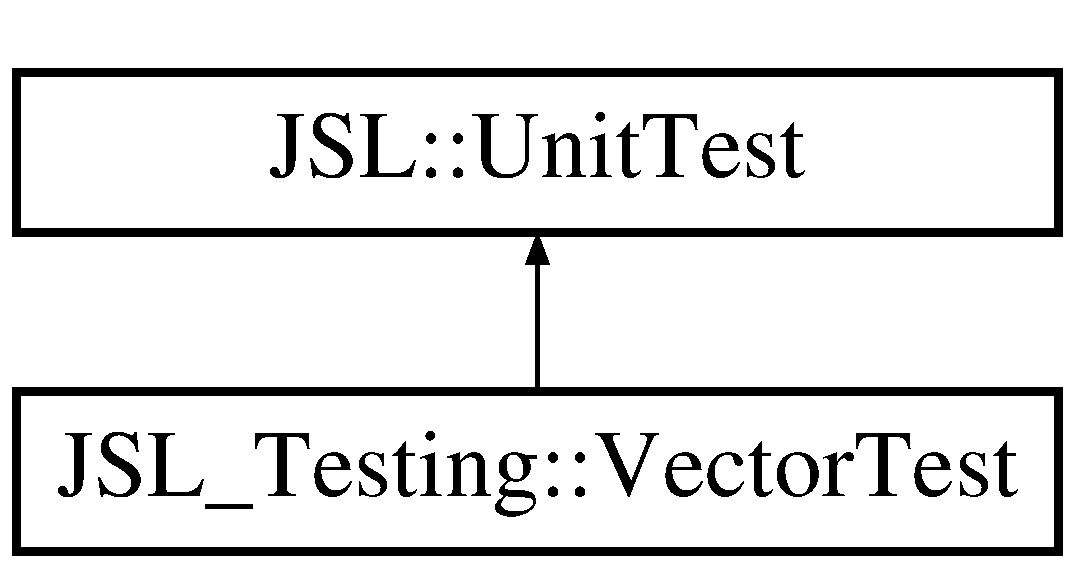
\includegraphics[height=2.000000cm]{classJSL__Testing_1_1VectorTest}
\end{center}
\end{figure}
\doxysubsection*{Public Member Functions}
\begin{DoxyCompactItemize}
\item 
\mbox{\hyperlink{classJSL__Testing_1_1VectorTest_a4750f287bc10a0df1f4f28cb84598bc2}{Vector\+Test}} ()
\item 
void \mbox{\hyperlink{classJSL__Testing_1_1VectorTest_ad79bb4654e6f7b59d31d7239ee0c2b82}{Run\+\_\+\+Test}} ()
\begin{DoxyCompactList}\small\item\em All children which want to take advantage of the \mbox{\hyperlink{classJSL_1_1UnitTest_aabec19b081be8a428f12e4b5e3dc2a9c}{Buffered\+Test()}} command should have the bulk of their testing within this command. \end{DoxyCompactList}\end{DoxyCompactItemize}
\doxysubsection*{Additional Inherited Members}


\doxysubsection{Constructor \& Destructor Documentation}
\mbox{\Hypertarget{classJSL__Testing_1_1VectorTest_a4750f287bc10a0df1f4f28cb84598bc2}\label{classJSL__Testing_1_1VectorTest_a4750f287bc10a0df1f4f28cb84598bc2}} 
\index{JSL\_Testing::VectorTest@{JSL\_Testing::VectorTest}!VectorTest@{VectorTest}}
\index{VectorTest@{VectorTest}!JSL\_Testing::VectorTest@{JSL\_Testing::VectorTest}}
\doxysubsubsection{\texorpdfstring{VectorTest()}{VectorTest()}}
{\footnotesize\ttfamily J\+S\+L\+\_\+\+Testing\+::\+Vector\+Test\+::\+Vector\+Test (\begin{DoxyParamCaption}{ }\end{DoxyParamCaption})\hspace{0.3cm}{\ttfamily [inline]}}



\doxysubsection{Member Function Documentation}
\mbox{\Hypertarget{classJSL__Testing_1_1VectorTest_ad79bb4654e6f7b59d31d7239ee0c2b82}\label{classJSL__Testing_1_1VectorTest_ad79bb4654e6f7b59d31d7239ee0c2b82}} 
\index{JSL\_Testing::VectorTest@{JSL\_Testing::VectorTest}!Run\_Test@{Run\_Test}}
\index{Run\_Test@{Run\_Test}!JSL\_Testing::VectorTest@{JSL\_Testing::VectorTest}}
\doxysubsubsection{\texorpdfstring{Run\_Test()}{Run\_Test()}}
{\footnotesize\ttfamily void J\+S\+L\+\_\+\+Testing\+::\+Vector\+Test\+::\+Run\+\_\+\+Test (\begin{DoxyParamCaption}{ }\end{DoxyParamCaption})\hspace{0.3cm}{\ttfamily [inline]}, {\ttfamily [virtual]}}



All children which want to take advantage of the \mbox{\hyperlink{classJSL_1_1UnitTest_aabec19b081be8a428f12e4b5e3dc2a9c}{Buffered\+Test()}} command should have the bulk of their testing within this command. 



Reimplemented from \mbox{\hyperlink{classJSL_1_1UnitTest_aa8369ab1ce2a537bff2ea7e1c8818490}{J\+S\+L\+::\+Unit\+Test}}.



The documentation for this class was generated from the following file\+:\begin{DoxyCompactItemize}
\item 
/home/jack/\+Documents/\+Work/\+Q\+Dynamics/lib/\+J\+S\+L/\+Testing/\mbox{\hyperlink{Testing__UnitTests_8h}{Testing\+\_\+\+Unit\+Tests.\+h}}\end{DoxyCompactItemize}

\chapter{File Documentation}
\hypertarget{Argument_8h}{}\section{/home/f/fraserj/\+Documents/\+Work/\+Q\+Dynamics/lib/\+J\+S\+L/\+Command\+Args/\+Argument.h File Reference}
\label{Argument_8h}\index{/home/f/fraserj/\+Documents/\+Work/\+Q\+Dynamics/lib/\+J\+S\+L/\+Command\+Args/\+Argument.\+h@{/home/f/fraserj/\+Documents/\+Work/\+Q\+Dynamics/lib/\+J\+S\+L/\+Command\+Args/\+Argument.\+h}}
{\ttfamily \#include $<$string$>$}\newline
{\ttfamily \#include $<$stdexcept$>$}\newline
{\ttfamily \#include \char`\"{}../\+File\+I\+O/\+File\+I\+O.\+h\char`\"{}}\newline
\subsection*{Data Structures}
\begin{DoxyCompactItemize}
\item 
class \hyperlink{classJSL_1_1ArgumentInterface}{J\+S\+L\+::\+Argument\+Interface}
\item 
class \hyperlink{classJSL_1_1Argument}{J\+S\+L\+::\+Argument$<$ T $>$}
\end{DoxyCompactItemize}
\subsection*{Namespaces}
\begin{DoxyCompactItemize}
\item 
 \hyperlink{namespaceJSL}{J\+SL}
\end{DoxyCompactItemize}

\hypertarget{CommandArgs_8h}{}\section{/home/f/fraserj/\+Documents/\+Work/\+Q\+Dynamics/lib/\+J\+S\+L/\+Command\+Args/\+Command\+Args.h File Reference}
\label{CommandArgs_8h}\index{/home/f/fraserj/\+Documents/\+Work/\+Q\+Dynamics/lib/\+J\+S\+L/\+Command\+Args/\+Command\+Args.\+h@{/home/f/fraserj/\+Documents/\+Work/\+Q\+Dynamics/lib/\+J\+S\+L/\+Command\+Args/\+Command\+Args.\+h}}
{\ttfamily \#include \char`\"{}Argument.\+h\char`\"{}}\newline

\hypertarget{FileIO_8h}{}\doxysection{/home/jack/\+Documents/\+Work/\+Q\+Dynamics/lib/\+J\+S\+L/\+File\+I\+O/\+File\+IO.h File Reference}
\label{FileIO_8h}\index{/home/jack/Documents/Work/QDynamics/lib/JSL/FileIO/FileIO.h@{/home/jack/Documents/Work/QDynamics/lib/JSL/FileIO/FileIO.h}}
{\ttfamily \#include \char`\"{}Line\+Reader.\+h\char`\"{}}\newline
{\ttfamily \#include \char`\"{}mkdir.\+h\char`\"{}}\newline
{\ttfamily \#include \char`\"{}rm.\+h\char`\"{}}\newline
{\ttfamily \#include \char`\"{}location\+Exists.\+h\char`\"{}}\newline
{\ttfamily \#include \char`\"{}file\+Writer.\+h\char`\"{}}\newline

\hypertarget{fileWriter_8h}{}\section{/home/f/fraserj/\+Documents/\+Work/\+Q\+Dynamics/lib/\+J\+S\+L/\+File\+I\+O/file\+Writer.h File Reference}
\label{fileWriter_8h}\index{/home/f/fraserj/\+Documents/\+Work/\+Q\+Dynamics/lib/\+J\+S\+L/\+File\+I\+O/file\+Writer.\+h@{/home/f/fraserj/\+Documents/\+Work/\+Q\+Dynamics/lib/\+J\+S\+L/\+File\+I\+O/file\+Writer.\+h}}
{\ttfamily \#include \char`\"{}string.\+h\char`\"{}}\newline
{\ttfamily \#include $<$fstream$>$}\newline
\subsection*{Namespaces}
\begin{DoxyCompactItemize}
\item 
 \hyperlink{namespaceJSL}{J\+SL}
\end{DoxyCompactItemize}
\subsection*{Functions}
\begin{DoxyCompactItemize}
\item 
void \hyperlink{namespaceJSL_a47d8cb112d513ee5a3ae38ca6a89743d}{J\+S\+L\+::initialise\+File} (const std\+::string \&filename)
\item 
void \hyperlink{namespaceJSL_a838b3a913896993bc008408d164ec19d}{J\+S\+L\+::write\+String\+To\+File} (const std\+::string \&filename, const std\+::string \&content)
\item 
{\footnotesize template$<$class T $>$ }\\void \hyperlink{namespaceJSL_a1d611217d83275af846cbc091ff98f53}{J\+S\+L\+::write\+Vector\+To\+File} (const std\+::string \&filename, const std\+::vector$<$ T $>$ \&content\+Vector, const std\+::string \&delimiter, bool include\+Terminal\+Line\+Break)
\item 
{\footnotesize template$<$class T $>$ }\\void \hyperlink{namespaceJSL_a8c08233b0cb834d4dcde1153b4b8c8c7}{J\+S\+L\+::write\+Matrix\+To\+File} (const std\+::string \&filename, const std\+::vector$<$ std\+::vector$<$ T $>$$>$ content\+Matrix, const std\+::string \&column\+Delimiter, const std\+::string \&row\+Delimiter)
\end{DoxyCompactItemize}

\hypertarget{LineReader_8h}{}\doxysection{/home/jack/\+Documents/\+Work/\+Q\+Dynamics/lib/\+J\+S\+L/\+File\+I\+O/\+Line\+Reader.h File Reference}
\label{LineReader_8h}\index{/home/jack/Documents/Work/QDynamics/lib/JSL/FileIO/LineReader.h@{/home/jack/Documents/Work/QDynamics/lib/JSL/FileIO/LineReader.h}}
{\ttfamily \#include $<$fstream$>$}\newline
{\ttfamily \#include $<$string$>$}\newline
{\ttfamily \#include $<$vector$>$}\newline
{\ttfamily \#include \char`\"{}../\+Strings/split.\+h\char`\"{}}\newline
\doxysubsection*{Macros}
\begin{DoxyCompactItemize}
\item 
\#define \mbox{\hyperlink{LineReader_8h_a5480fba013891b2f3033cc97d5d8edf4}{for\+Line\+In}}(macro\+File\+Name, ...)
\item 
\#define \mbox{\hyperlink{LineReader_8h_abdfa973ea7dd7efb90a74e8ec636f5ed}{for\+Line\+Vector\+In}}(macro\+File\+Name,  token, ...)
\end{DoxyCompactItemize}


\doxysubsection{Macro Definition Documentation}
\mbox{\Hypertarget{LineReader_8h_a5480fba013891b2f3033cc97d5d8edf4}\label{LineReader_8h_a5480fba013891b2f3033cc97d5d8edf4}} 
\index{LineReader.h@{LineReader.h}!forLineIn@{forLineIn}}
\index{forLineIn@{forLineIn}!LineReader.h@{LineReader.h}}
\doxysubsubsection{\texorpdfstring{forLineIn}{forLineIn}}
{\footnotesize\ttfamily \#define for\+Line\+In(\begin{DoxyParamCaption}\item[{}]{macro\+File\+Name,  }\item[{}]{... }\end{DoxyParamCaption})}

{\bfseries Value\+:}
\begin{DoxyCode}{0}
\DoxyCodeLine{\{                               \(\backslash\)}
\DoxyCodeLine{    do                          \(\backslash\)}
\DoxyCodeLine{    \{                           \(\backslash\)}
\DoxyCodeLine{        std::ifstream macroFile(macroFileName); \(\backslash\)}
\DoxyCodeLine{        if (!macroFile.is\_open())   \(\backslash\)}
\DoxyCodeLine{        \{                           \(\backslash\)}
\DoxyCodeLine{            std::cout << \textcolor{stringliteral}{"\(\backslash\)n\(\backslash\)nERROR: Could not find the file '"} << macroFileName << \textcolor{stringliteral}{".\(\backslash\)n\(\backslash\)nPlease provide a valid filepath.\(\backslash\)n\(\backslash\)n "} << std::endl;  \(\backslash\)}
\DoxyCodeLine{            exit(1);                \(\backslash\)}
\DoxyCodeLine{        \}                           \(\backslash\)}
\DoxyCodeLine{        std::string FILE\_LINE;              \(\backslash\)}
\DoxyCodeLine{        while (getline(macroFile,FILE\_LINE))    \(\backslash\)}
\DoxyCodeLine{        \{                           \(\backslash\)}
\DoxyCodeLine{            \_\_VA\_ARGS\_\_             \(\backslash\)}
\DoxyCodeLine{        \}                           \(\backslash\)}
\DoxyCodeLine{        macroFile.close();          \(\backslash\)}
\DoxyCodeLine{    \} \textcolor{keywordflow}{while}(0);                     \(\backslash\)}
\DoxyCodeLine{\}                                   \(\backslash\)}

\end{DoxyCode}
Iterates through the file line-\/by-\/line (until E\+OF), saving the current line to {\ttfamily std\+::string F\+I\+L\+E\+\_\+\+L\+I\+NE} 
\begin{DoxyParams}{Parameters}
{\em macro\+File\+Name} & The target file to search through \\
\hline
{\em ...} & A custom block of C++ code which executes on every line of the file. You may use any externally defined variables within this block. \\
\hline
\end{DoxyParams}
\begin{DoxyReturn}{Returns}
Current line is accessible via the variable {\ttfamily std\+::string F\+I\+L\+E\+\_\+\+L\+I\+NE}. If the file does not exist, throws an {\ttfamily exit(1)} command 
\end{DoxyReturn}
\mbox{\Hypertarget{LineReader_8h_abdfa973ea7dd7efb90a74e8ec636f5ed}\label{LineReader_8h_abdfa973ea7dd7efb90a74e8ec636f5ed}} 
\index{LineReader.h@{LineReader.h}!forLineVectorIn@{forLineVectorIn}}
\index{forLineVectorIn@{forLineVectorIn}!LineReader.h@{LineReader.h}}
\doxysubsubsection{\texorpdfstring{forLineVectorIn}{forLineVectorIn}}
{\footnotesize\ttfamily \#define for\+Line\+Vector\+In(\begin{DoxyParamCaption}\item[{}]{macro\+File\+Name,  }\item[{}]{token,  }\item[{}]{... }\end{DoxyParamCaption})}

{\bfseries Value\+:}
\begin{DoxyCode}{0}
\DoxyCodeLine{\{                               \(\backslash\)}
\DoxyCodeLine{    forLineIn(macroFileName,                    \(\backslash\)}
\DoxyCodeLine{            std::vector<std::string> FILE\_LINE\_VECTOR = \mbox{\hyperlink{namespaceJSL_a34a7ba28084b304e97a707c653dce887}{JSL::split}}(FILE\_LINE,token);  \(\backslash\)}
\DoxyCodeLine{            \_\_VA\_ARGS\_\_;                \(\backslash\)}
\DoxyCodeLine{    );                                  \(\backslash\)}
\DoxyCodeLine{\}}

\end{DoxyCode}
Iterates through the file line-\/by-\/line (until E\+OF), saving the current line to {\ttfamily std\+::string F\+I\+L\+E\+\_\+\+L\+I\+NE}, and then tokenises it using \mbox{\hyperlink{namespaceJSL_a34a7ba28084b304e97a707c653dce887}{split()}}, based on the chosen delimiter, saving it to {\ttfamily std\+::vector$<$std\+::string$>$$>$ F\+I\+L\+E\+\_\+\+L\+I\+N\+E\+\_\+\+V\+E\+C\+T\+OR} 
\begin{DoxyParams}{Parameters}
{\em macro\+File\+Name} & The target file to search through \\
\hline
{\em token} & The delimiter used to break up {\ttfamily F\+I\+L\+E\+\_\+\+L\+I\+NE} into {\ttfamily F\+I\+L\+E\+\_\+\+L\+I\+N\+E\+\_\+\+V\+E\+C\+T\+OR} \\
\hline
{\em ...} & A custom block of C++ code which executes on every line of the file. You may use any externally defined variables within this block. \\
\hline
\end{DoxyParams}
\begin{DoxyReturn}{Returns}
Current line is accessible via the variable {\ttfamily std\+::string F\+I\+L\+E\+\_\+\+L\+I\+NE} and {\ttfamily std\+::vector$<$std\+::string$>$$>$ F\+I\+L\+E\+\_\+\+L\+I\+N\+E\+\_\+\+V\+E\+C\+T\+OR}. If the file does not exist, throws an {\ttfamily exit(1)} command 
\end{DoxyReturn}

\hypertarget{locationExists_8h}{}\section{/home/f/fraserj/\+Documents/\+Work/\+Q\+Dynamics/lib/\+J\+S\+L/\+File\+I\+O/location\+Exists.h File Reference}
\label{locationExists_8h}\index{/home/f/fraserj/\+Documents/\+Work/\+Q\+Dynamics/lib/\+J\+S\+L/\+File\+I\+O/location\+Exists.\+h@{/home/f/fraserj/\+Documents/\+Work/\+Q\+Dynamics/lib/\+J\+S\+L/\+File\+I\+O/location\+Exists.\+h}}
{\ttfamily \#include $<$string$>$}\newline
{\ttfamily \#include $<$sys/stat.\+h$>$}\newline
\subsection*{Namespaces}
\begin{DoxyCompactItemize}
\item 
 \hyperlink{namespaceJSL}{J\+SL}
\end{DoxyCompactItemize}
\subsection*{Functions}
\begin{DoxyCompactItemize}
\item 
bool \hyperlink{namespaceJSL_a1752cd7c6e1134da51e9307527e0d788}{J\+S\+L\+::location\+Exists} (const std\+::string \&filename)
\end{DoxyCompactItemize}

\hypertarget{mkdir_8h}{}\section{/home/f/fraserj/\+Documents/\+Work/\+Q\+Dynamics/lib/\+J\+S\+L/\+File\+I\+O/mkdir.h File Reference}
\label{mkdir_8h}\index{/home/f/fraserj/\+Documents/\+Work/\+Q\+Dynamics/lib/\+J\+S\+L/\+File\+I\+O/mkdir.\+h@{/home/f/fraserj/\+Documents/\+Work/\+Q\+Dynamics/lib/\+J\+S\+L/\+File\+I\+O/mkdir.\+h}}
{\ttfamily \#include $<$dirent.\+h$>$}\newline
{\ttfamily \#include $<$string$>$}\newline
{\ttfamily \#include \char`\"{}location\+Exists.\+h\char`\"{}}\newline
\subsection*{Data Structures}
\begin{DoxyCompactItemize}
\item 
struct \hyperlink{structJSL_1_1mkdirReturn}{J\+S\+L\+::mkdir\+Return}
\begin{DoxyCompactList}\small\item\em A wrapper for the return type of mkdir\+Safely() \end{DoxyCompactList}\end{DoxyCompactItemize}
\subsection*{Namespaces}
\begin{DoxyCompactItemize}
\item 
 \hyperlink{namespaceJSL}{J\+SL}
\end{DoxyCompactItemize}
\subsection*{Functions}
\begin{DoxyCompactItemize}
\item 
mkdir\+Return \hyperlink{namespaceJSL_abf525d02b8c49f21ef7faa68b7571f93}{J\+S\+L\+::mkdir} (std\+::string directory)
\end{DoxyCompactItemize}

\hypertarget{rm_8h}{}\section{/home/f/fraserj/\+Documents/\+Work/\+Q\+Dynamics/lib/\+J\+S\+L/\+File\+I\+O/rm.h File Reference}
\label{rm_8h}\index{/home/f/fraserj/\+Documents/\+Work/\+Q\+Dynamics/lib/\+J\+S\+L/\+File\+I\+O/rm.\+h@{/home/f/fraserj/\+Documents/\+Work/\+Q\+Dynamics/lib/\+J\+S\+L/\+File\+I\+O/rm.\+h}}
{\ttfamily \#include $<$dirent.\+h$>$}\newline
{\ttfamily \#include $<$string$>$}\newline
{\ttfamily \#include \char`\"{}location\+Exists.\+h\char`\"{}}\newline
{\ttfamily \#include $<$stdexcept$>$}\newline
\subsection*{Namespaces}
\begin{DoxyCompactItemize}
\item 
 \hyperlink{namespaceJSL}{J\+SL}
\end{DoxyCompactItemize}
\subsection*{Functions}
\begin{DoxyCompactItemize}
\item 
void \hyperlink{namespaceJSL_ae48b92e64fb9d321121df976b770efa6}{J\+S\+L\+::rm} (std\+::string location, bool recursive)
\end{DoxyCompactItemize}

\hypertarget{JSL_8h}{}\doxysection{/home/jack/\+Documents/\+Work/\+Q\+Dynamics/lib/\+J\+S\+L/\+J\+SL.h File Reference}
\label{JSL_8h}\index{/home/jack/Documents/Work/QDynamics/lib/JSL/JSL.h@{/home/jack/Documents/Work/QDynamics/lib/JSL/JSL.h}}
{\ttfamily \#include \char`\"{}File\+I\+O/\+File\+I\+O.\+h\char`\"{}}\newline
{\ttfamily \#include \char`\"{}Strings/\+Strings.\+h\char`\"{}}\newline
{\ttfamily \#include \char`\"{}Command\+Args/\+Command\+Args.\+h\char`\"{}}\newline
{\ttfamily \#include \char`\"{}Maths/\+Maths.\+h\char`\"{}}\newline
{\ttfamily \#include \char`\"{}Testing/\+Testing.\+h\char`\"{}}\newline

\hypertarget{Maths_8h}{}\doxysection{/home/jack/\+Documents/\+Work/\+Q\+Dynamics/lib/\+J\+S\+L/\+Maths/\+Maths.h File Reference}
\label{Maths_8h}\index{/home/jack/Documents/Work/QDynamics/lib/JSL/Maths/Maths.h@{/home/jack/Documents/Work/QDynamics/lib/JSL/Maths/Maths.h}}
{\ttfamily \#include \char`\"{}vector.\+h\char`\"{}}\newline
{\ttfamily \#include \char`\"{}matrix.\+h\char`\"{}}\newline

\hypertarget{matrix_8h}{}\doxysection{/home/jack/\+Documents/\+Work/\+Q\+Dynamics/lib/\+J\+S\+L/\+Maths/matrix.h File Reference}
\label{matrix_8h}\index{/home/jack/Documents/Work/QDynamics/lib/JSL/Maths/matrix.h@{/home/jack/Documents/Work/QDynamics/lib/JSL/Maths/matrix.h}}
{\ttfamily \#include $<$vector$>$}\newline
{\ttfamily \#include $<$stdexcept$>$}\newline
{\ttfamily \#include $<$string.\+h$>$}\newline
{\ttfamily \#include $<$iostream$>$}\newline
{\ttfamily \#include $<$math.\+h$>$}\newline
{\ttfamily \#include \char`\"{}vector.\+h\char`\"{}}\newline
\doxysubsection*{Data Structures}
\begin{DoxyCompactItemize}
\item 
class \mbox{\hyperlink{classJSL_1_1Matrix}{J\+S\+L\+::\+Matrix}}
\end{DoxyCompactItemize}
\doxysubsection*{Namespaces}
\begin{DoxyCompactItemize}
\item 
 \mbox{\hyperlink{namespaceJSL}{J\+SL}}
\end{DoxyCompactItemize}
\doxysubsection*{Functions}
\begin{DoxyCompactItemize}
\item 
bool \mbox{\hyperlink{namespaceJSL_a682c8bb3fff54370f38dcb16794fc7c5}{J\+S\+L\+::operator==}} (const Matrix \&lhs, const Matrix \&rhs)
\item 
bool \mbox{\hyperlink{namespaceJSL_a8b19814a4b6cb667d1e27133acc38513}{J\+S\+L\+::operator!=}} (const Matrix \&lhs, const Matrix \&rhs)
\item 
bool \mbox{\hyperlink{namespaceJSL_a38d1bbf23dc57ec028ea8d91a9688957}{J\+S\+L\+::\+Matrix\+Sizes\+Equal}} (const Matrix \&m1, const Matrix \&m2)
\item 
Matrix \mbox{\hyperlink{namespaceJSL_ad1bcc74167579ecff71209bf8c9c47a3}{J\+S\+L\+::operator+}} (const Matrix \&lhs, const Matrix \&rhs)
\begin{DoxyCompactList}\small\item\em Performs obvious matrix addition (a+b)\+\_\+ij = a\+\_\+ij + b\+\_\+ij. Throws an error if the matrices are not the same size. \end{DoxyCompactList}\item 
Matrix \mbox{\hyperlink{namespaceJSL_a4f1a2a224c7f6a8c57627b03594cd89f}{J\+S\+L\+::operator-\/}} (const Matrix \&lhs, const Matrix \&rhs)
\begin{DoxyCompactList}\small\item\em Performs obvious matrix subtraction (a-\/b)\+\_\+ij = a\+\_\+ij -\/ b\+\_\+ij. Throws an error if the matrices are not the same size. \end{DoxyCompactList}\item 
Matrix \mbox{\hyperlink{namespaceJSL_ad779a68a2d565490f76dd16adfc3091e}{J\+S\+L\+::operator+}} (const Matrix \&lhs, const double \&scalar)
\begin{DoxyCompactList}\small\item\em Adds the value of scalar to every element in the matrix. \end{DoxyCompactList}\item 
Matrix \mbox{\hyperlink{namespaceJSL_a95d670e99aed43f857d8ba5e6f3d7897}{J\+S\+L\+::operator$\ast$}} (const Matrix \&lhs, const Matrix \&rhs)
\item 
Vector \mbox{\hyperlink{namespaceJSL_a823f5e48d384320644698917c0a1c85c}{J\+S\+L\+::operator$\ast$}} (const Matrix \&lhs, const Vector \&rhs)
\item 
Matrix \mbox{\hyperlink{namespaceJSL_a5f6c1988cf84b088617e0f12fc1e98da}{J\+S\+L\+::operator+}} (const double \&scalar, const Matrix \&rhs)
\begin{DoxyCompactList}\small\item\em Exactly equivalent to \mbox{\hyperlink{namespaceJSL_ad779a68a2d565490f76dd16adfc3091e}{J\+S\+L\+::operator+(const Matrix \&lhs, const double \&scalar)}}, just swapped around. \end{DoxyCompactList}\item 
Matrix \mbox{\hyperlink{namespaceJSL_a6d5304adbdadcb062246266f4ece24a1}{J\+S\+L\+::operator-\/}} (const Matrix \&lhs, const double \&scalar)
\begin{DoxyCompactList}\small\item\em Subtracts the value of scalar to every element in the \mbox{\hyperlink{classJSL_1_1Matrix}{Matrix}}. \end{DoxyCompactList}\item 
Matrix \mbox{\hyperlink{namespaceJSL_a80fcd230a03dd81f1c37fec030619bf9}{J\+S\+L\+::operator$\ast$}} (const double \&scalar, const Matrix \&rhs)
\begin{DoxyCompactList}\small\item\em Naive element-\/wise scalar multiplication. \end{DoxyCompactList}\item 
Matrix \mbox{\hyperlink{namespaceJSL_a69548e09ba5835ee87ac4d28907b5435}{J\+S\+L\+::operator$\ast$}} (const Matrix \&lhs, const double \&scalar)
\begin{DoxyCompactList}\small\item\em Alias of \mbox{\hyperlink{namespaceJSL_a5f6c1988cf84b088617e0f12fc1e98da}{J\+S\+L\+::operator+(const double \&scalar,const Matrix \&rhs)}} with the operation order swapped around. \end{DoxyCompactList}\item 
Matrix \mbox{\hyperlink{namespaceJSL_ab1f3153179f59c59a0c2a5e553889eb1}{J\+S\+L\+::operator/}} (const Matrix \&lhs, const double \&scalar)
\begin{DoxyCompactList}\small\item\em Essentially an alias for \mbox{\hyperlink{namespaceJSL_a5f6c1988cf84b088617e0f12fc1e98da}{J\+S\+L\+::operator+(const double \&scalar,const Matrix \&rhs)}} with the scalar set to one-\/over itself, i.\+e. pointwise division of the provided matrix. \end{DoxyCompactList}\item 
Matrix \mbox{\hyperlink{namespaceJSL_aebaffa5dc8073b816908a9708a36b7bf}{J\+S\+L\+::operator-\/}} (const double \&scalar, const Matrix \&rhs)
\begin{DoxyCompactList}\small\item\em A slightly odd operation (included for completeness) -\/ adds the value of scalar to the negative of the elements of the vector. \end{DoxyCompactList}\item 
std\+::ostream \& \mbox{\hyperlink{namespaceJSL_a91df7f3a77ef2e000058e0f58efb99e6}{J\+S\+L\+::operator$<$$<$}} (std\+::ostream \&os, const Matrix \&obj)
\begin{DoxyCompactList}\small\item\em Calls \mbox{\hyperlink{classJSL_1_1Matrix_abcf44559767ab6939851f0d3b60c6fa8}{J\+S\+L\+::\+Matrix\+::to\+\_\+string()}} and then passes it to the provided stream, enabling sweet, smooth output such as std\+::cout $<$$<$ M $<$$<$ std\+::endl. \end{DoxyCompactList}\end{DoxyCompactItemize}

\hypertarget{Q__temp_8h}{}\section{/home/f/fraserj/\+Documents/\+Work/\+Q\+Dynamics/lib/\+J\+S\+L/\+Maths/\+Q\+\_\+temp.h File Reference}
\label{Q__temp_8h}\index{/home/f/fraserj/\+Documents/\+Work/\+Q\+Dynamics/lib/\+J\+S\+L/\+Maths/\+Q\+\_\+temp.\+h@{/home/f/fraserj/\+Documents/\+Work/\+Q\+Dynamics/lib/\+J\+S\+L/\+Maths/\+Q\+\_\+temp.\+h}}
{\ttfamily \#include $<$vector$>$}\newline
{\ttfamily \#include $<$stdexcept$>$}\newline
{\ttfamily \#include $<$string.\+h$>$}\newline
{\ttfamily \#include $<$iostream$>$}\newline
{\ttfamily \#include $<$math.\+h$>$}\newline
{\ttfamily \#include \char`\"{}vector.\+h\char`\"{}}\newline
{\ttfamily \#include \char`\"{}matrix.\+h\char`\"{}}\newline
\subsection*{Data Structures}
\begin{DoxyCompactItemize}
\item 
class \hyperlink{classJSL_1_1Quaternion}{J\+S\+L\+::\+Quaternion}
\end{DoxyCompactItemize}
\subsection*{Namespaces}
\begin{DoxyCompactItemize}
\item 
 \hyperlink{namespaceJSL}{J\+SL}
\end{DoxyCompactItemize}
\subsection*{Functions}
\begin{DoxyCompactItemize}
\item 
Quaternion \hyperlink{namespaceJSL_aff956bc38fdc0a19f41e202699560dff}{J\+S\+L\+::operator$\ast$} (const Quaternion \&lhs, const Quaternion \&rhs)
\item 
Quaternion \hyperlink{namespaceJSL_a87842870ba7998a0ec521782b2d2f621}{J\+S\+L\+::operator$\ast$} (const \hyperlink{classJSL_1_1Matrix}{J\+S\+L\+::\+Matrix} \&lhs, const Quaternion \&rhs)
\item 
Quaternion \hyperlink{namespaceJSL_a68fed2d9fae3ec9612dd8e8282cf1336}{J\+S\+L\+::operator/} (const Quaternion \&lhs, const Quaternion \&rhs)
\item 
Quaternion \hyperlink{namespaceJSL_a943a21cab5e9abe4331b20d37cd3f8a1}{J\+S\+L\+::exp} (const \hyperlink{classJSL_1_1Quaternion}{J\+S\+L\+::\+Quaternion} \&a)
\end{DoxyCompactItemize}

\hypertarget{vector_8h}{}\section{/home/f/fraserj/\+Documents/\+Work/\+Q\+Dynamics/lib/\+J\+S\+L/\+Maths/vector.h File Reference}
\label{vector_8h}\index{/home/f/fraserj/\+Documents/\+Work/\+Q\+Dynamics/lib/\+J\+S\+L/\+Maths/vector.\+h@{/home/f/fraserj/\+Documents/\+Work/\+Q\+Dynamics/lib/\+J\+S\+L/\+Maths/vector.\+h}}
{\ttfamily \#include $<$vector$>$}\newline
{\ttfamily \#include $<$stdexcept$>$}\newline
{\ttfamily \#include $<$string.\+h$>$}\newline
{\ttfamily \#include $<$iostream$>$}\newline
{\ttfamily \#include $<$math.\+h$>$}\newline
\subsection*{Data Structures}
\begin{DoxyCompactItemize}
\item 
class \hyperlink{classJSL_1_1Vector}{J\+S\+L\+::\+Vector}
\end{DoxyCompactItemize}
\subsection*{Namespaces}
\begin{DoxyCompactItemize}
\item 
 \hyperlink{namespaceJSL}{J\+SL}
\end{DoxyCompactItemize}
\subsection*{Functions}
\begin{DoxyCompactItemize}
\item 
double \hyperlink{namespaceJSL_aeae64b7e0cfdc1ab5f35cca90c32d9f6}{J\+S\+L\+::\+Vector\+Dot\+Product} (const Vector \&lhs, const Vector \&rhs)
\begin{DoxyCompactList}\small\item\em The standard dot product on R$^\wedge$n. \end{DoxyCompactList}\item 
Vector \hyperlink{namespaceJSL_aa7816eb0cd81b74241ce460237990e70}{J\+S\+L\+::\+Vector\+Cross\+Product} (const Vector \&lhs, const Vector \&rhs)
\begin{DoxyCompactList}\small\item\em The standard cross product -- only defined on R$^\wedge$3 (throws an error else) \end{DoxyCompactList}\item 
double \hyperlink{namespaceJSL_a09355c91f84fd99d4634bf9189fef51d}{J\+S\+L\+::\+Angle\+Between\+Vectors} (const Vector \&lhs, const Vector \&rhs)
\begin{DoxyCompactList}\small\item\em Uses \hyperlink{classJSL_1_1Vector_aa8af717591f5548ff471b6e4b28d7f9c}{Vector\+::\+Norm()} and \hyperlink{namespaceJSL_aeae64b7e0cfdc1ab5f35cca90c32d9f6}{Vector\+Dot\+Product()} to extract an angle between the vectors. \end{DoxyCompactList}\item 
bool \hyperlink{namespaceJSL_a7fad54be308ccb76f68933d91c3c542f}{J\+S\+L\+::operator==} (const Vector \&lhs, const Vector \&rhs)
\item 
bool \hyperlink{namespaceJSL_a394a4f9cee0747c76d1190b0365c7b5a}{J\+S\+L\+::operator!=} (const Vector \&lhs, const Vector \&rhs)
\item 
Vector \hyperlink{namespaceJSL_ae6530b77174d0dfae8e0d6e2a810f672}{J\+S\+L\+::operator+} (const Vector \&lhs, const Vector \&rhs)
\begin{DoxyCompactList}\small\item\em Performs obvious vector addition (a+b)\+\_\+i = a\+\_\+i + b\+\_\+i. Throws an error if the vectors are not the same size. \end{DoxyCompactList}\item 
Vector \hyperlink{namespaceJSL_a1d8393f2865dc23e7975ad041e341ba5}{J\+S\+L\+::operator-\/} (const Vector \&lhs, const Vector \&rhs)
\begin{DoxyCompactList}\small\item\em Performs obvious vector subtraction (a-\/b)\+\_\+i = a\+\_\+i -\/ b\+\_\+i. Throws an error if the vectors are not the same size. \end{DoxyCompactList}\item 
Vector \hyperlink{namespaceJSL_a4b293e2ac3df51113e80022cb3c2ac99}{J\+S\+L\+::operator+} (const Vector \&lhs, const double \&scalar)
\begin{DoxyCompactList}\small\item\em Adds the value of scalar to every element in the vector. \end{DoxyCompactList}\item 
Vector \hyperlink{namespaceJSL_ac5ceabb8b9e657c5e2d0faf9b20a36e8}{J\+S\+L\+::operator+} (const double \&scalar, const Vector \&rhs)
\begin{DoxyCompactList}\small\item\em Exactly equivalent to \hyperlink{namespaceJSL_a4b293e2ac3df51113e80022cb3c2ac99}{J\+S\+L\+::operator+(const Vector \&lhs, const double \&scalar)}, just swapped around. \end{DoxyCompactList}\item 
Vector \hyperlink{namespaceJSL_ac6bd9311dd73aa6227d826bdb94e748d}{J\+S\+L\+::operator-\/} (const Vector \&lhs, const double \&scalar)
\begin{DoxyCompactList}\small\item\em Subtracts the value of scalar to every element in the vector. \end{DoxyCompactList}\item 
Vector \hyperlink{namespaceJSL_ab3d17c5cc03a2048e8637d2054fbc138}{J\+S\+L\+::operator-\/} (const double \&scalar, const Vector \&rhs)
\begin{DoxyCompactList}\small\item\em A slightly odd operation (included for completeness) -\/ adds the value of scalar to the negative of the elements of the vector. \end{DoxyCompactList}\item 
Vector \hyperlink{namespaceJSL_ab4eefbed468f275164855895335b8a29}{J\+S\+L\+::operator$\ast$} (const double \&scalar, const Vector \&rhs)
\begin{DoxyCompactList}\small\item\em Naive element-\/wise scalar multiplication. \end{DoxyCompactList}\item 
Vector \hyperlink{namespaceJSL_afc5e092de4a9bdc5795d40ee0f51c7b9}{J\+S\+L\+::operator$\ast$} (const Vector \&lhs, const double \&scalar)
\begin{DoxyCompactList}\small\item\em Alias of \hyperlink{namespaceJSL_ac5ceabb8b9e657c5e2d0faf9b20a36e8}{J\+S\+L\+::operator+(const double \&scalar,const Vector \&rhs)} with the operation order swapped around. \end{DoxyCompactList}\item 
Vector \hyperlink{namespaceJSL_a1427fd44260592b7d65d27946969fba1}{J\+S\+L\+::operator/} (const Vector \&lhs, const double \&scalar)
\begin{DoxyCompactList}\small\item\em Essentially an alias for \hyperlink{namespaceJSL_ac5ceabb8b9e657c5e2d0faf9b20a36e8}{J\+S\+L\+::operator+(const double \&scalar,const Vector \&rhs)} with the scalar set to one-\/over itself, i.\+e. pointwise division of the provided vector. \end{DoxyCompactList}\item 
Vector \hyperlink{namespaceJSL_a6fd4487b0a8ac5713df4a37079287913}{J\+S\+L\+::\+Hadamard} (const Vector \&lhs, const Vector \&rhs)
\begin{DoxyCompactList}\small\item\em Executes the pointwise (Hadamard) product of two vectors. \end{DoxyCompactList}\item 
std\+::ostream \& \hyperlink{namespaceJSL_ad9900d0292867da361ddb3f1200a1f99}{J\+S\+L\+::operator$<$$<$} (std\+::ostream \&os, const Vector \&obj)
\begin{DoxyCompactList}\small\item\em Calls \hyperlink{classJSL_1_1Vector_a73579b4a194cc924341806a5d9ea3817}{J\+S\+L\+::\+Vector\+::to\+\_\+string()} and then passes it to the provided stream, enabling sweet, smooth output such as std\+::cout $<$$<$ v1 $<$$<$ std\+::endl. \end{DoxyCompactList}\end{DoxyCompactItemize}

\hypertarget{split_8h}{}\section{/home/f/fraserj/\+Documents/\+Work/\+Q\+Dynamics/lib/\+J\+S\+L/\+Strings/split.h File Reference}
\label{split_8h}\index{/home/f/fraserj/\+Documents/\+Work/\+Q\+Dynamics/lib/\+J\+S\+L/\+Strings/split.\+h@{/home/f/fraserj/\+Documents/\+Work/\+Q\+Dynamics/lib/\+J\+S\+L/\+Strings/split.\+h}}
{\ttfamily \#include $<$string$>$}\newline
{\ttfamily \#include $<$vector$>$}\newline
{\ttfamily \#include $<$sstream$>$}\newline
\subsection*{Namespaces}
\begin{DoxyCompactItemize}
\item 
 \hyperlink{namespaceJSL}{J\+SL}
\end{DoxyCompactItemize}
\subsection*{Functions}
\begin{DoxyCompactItemize}
\item 
std\+::vector$<$ std\+::string $>$ \hyperlink{namespaceJSL_a34a7ba28084b304e97a707c653dce887}{J\+S\+L\+::split} (const std\+::string \&s, char delimiter)
\end{DoxyCompactItemize}

\hypertarget{Strings_8h}{}\section{/home/f/fraserj/\+Documents/\+Work/\+Q\+Dynamics/lib/\+J\+S\+L/\+Strings/\+Strings.h File Reference}
\label{Strings_8h}\index{/home/f/fraserj/\+Documents/\+Work/\+Q\+Dynamics/lib/\+J\+S\+L/\+Strings/\+Strings.\+h@{/home/f/fraserj/\+Documents/\+Work/\+Q\+Dynamics/lib/\+J\+S\+L/\+Strings/\+Strings.\+h}}
{\ttfamily \#include \char`\"{}split.\+h\char`\"{}}\newline
{\ttfamily \#include \char`\"{}Time.\+h\char`\"{}}\newline

\hypertarget{Time_8h}{}\section{/home/f/fraserj/\+Documents/\+Work/\+Q\+Dynamics/lib/\+J\+S\+L/\+Strings/\+Time.h File Reference}
\label{Time_8h}\index{/home/f/fraserj/\+Documents/\+Work/\+Q\+Dynamics/lib/\+J\+S\+L/\+Strings/\+Time.\+h@{/home/f/fraserj/\+Documents/\+Work/\+Q\+Dynamics/lib/\+J\+S\+L/\+Strings/\+Time.\+h}}
{\ttfamily \#include $<$chrono$>$}\newline
{\ttfamily \#include $<$string$>$}\newline
{\ttfamily \#include $<$sstream$>$}\newline
{\ttfamily \#include $<$vector$>$}\newline
{\ttfamily \#include $<$iostream$>$}\newline
\subsection*{Namespaces}
\begin{DoxyCompactItemize}
\item 
 \hyperlink{namespaceJSL}{J\+SL}
\end{DoxyCompactItemize}
\subsection*{Functions}
\begin{DoxyCompactItemize}
\item 
std\+::string \hyperlink{namespaceJSL_ae58b7096986a16b70a27e1609eff3014}{J\+S\+L\+::\+Current\+Time} ()
\item 
std\+::string \hyperlink{namespaceJSL_ad7ff2220bbab0294b95b9aa85332a222}{J\+S\+L\+::\+Format\+Duration} (int time\+In\+Seconds)
\item 
std\+::string \hyperlink{namespaceJSL_ae7af96a0311784e019209221335f76d9}{J\+S\+L\+::\+Format\+Clock} (std\+::chrono\+::time\+\_\+point$<$ std\+::chrono\+::system\+\_\+clock $>$ start, std\+::chrono\+::time\+\_\+point$<$ std\+::chrono\+::system\+\_\+clock $>$ end)
\end{DoxyCompactItemize}

\hypertarget{Testing_8h}{}\doxysection{/home/jack/\+Documents/\+Work/\+Q\+Dynamics/lib/\+J\+S\+L/\+Testing/\+Testing.h File Reference}
\label{Testing_8h}\index{/home/jack/Documents/Work/QDynamics/lib/JSL/Testing/Testing.h@{/home/jack/Documents/Work/QDynamics/lib/JSL/Testing/Testing.h}}
{\ttfamily \#include \char`\"{}Unit\+Test.\+h\char`\"{}}\newline
{\ttfamily \#include \char`\"{}Testing\+\_\+\+Unit\+Tests.\+h\char`\"{}}\newline

\hypertarget{Testing__UnitTests_8h}{}\section{/home/f/fraserj/\+Documents/\+Work/\+Q\+Dynamics/lib/\+J\+S\+L/\+Testing/\+Testing\+\_\+\+Unit\+Tests.h File Reference}
\label{Testing__UnitTests_8h}\index{/home/f/fraserj/\+Documents/\+Work/\+Q\+Dynamics/lib/\+J\+S\+L/\+Testing/\+Testing\+\_\+\+Unit\+Tests.\+h@{/home/f/fraserj/\+Documents/\+Work/\+Q\+Dynamics/lib/\+J\+S\+L/\+Testing/\+Testing\+\_\+\+Unit\+Tests.\+h}}
{\ttfamily \#include \char`\"{}../\+J\+S\+L.\+h\char`\"{}}\newline
{\ttfamily \#include $<$cmath$>$}\newline
\subsection*{Data Structures}
\begin{DoxyCompactItemize}
\item 
class \hyperlink{classJSL__Testing_1_1MetaTest}{J\+S\+L\+\_\+\+Testing\+::\+Meta\+Test}
\item 
class \hyperlink{classJSL__Testing_1_1StringTest}{J\+S\+L\+\_\+\+Testing\+::\+String\+Test}
\item 
class \hyperlink{classJSL__Testing_1_1IOTest}{J\+S\+L\+\_\+\+Testing\+::\+I\+O\+Test}
\item 
class \hyperlink{classJSL__Testing_1_1ArgumentTest}{J\+S\+L\+\_\+\+Testing\+::\+Argument\+Test}
\item 
class \hyperlink{classJSL__Testing_1_1VectorTest}{J\+S\+L\+\_\+\+Testing\+::\+Vector\+Test}
\item 
class \hyperlink{classJSL__Testing_1_1MatrixTest}{J\+S\+L\+\_\+\+Testing\+::\+Matrix\+Test}
\end{DoxyCompactItemize}
\subsection*{Namespaces}
\begin{DoxyCompactItemize}
\item 
 \hyperlink{namespaceJSL__Testing}{J\+S\+L\+\_\+\+Testing}
\end{DoxyCompactItemize}
\subsection*{Functions}
\begin{DoxyCompactItemize}
\item 
void \hyperlink{namespaceJSL__Testing_a509a70d20fdc2e9975d9b0b8ae424ef1}{J\+S\+L\+\_\+\+Testing\+::\+Run\+All\+Tests} ()
\end{DoxyCompactItemize}

\hypertarget{UnitTest_8h}{}\section{/home/f/fraserj/\+Documents/\+Work/\+Q\+Dynamics/lib/\+J\+S\+L/\+Testing/\+Unit\+Test.h File Reference}
\label{UnitTest_8h}\index{/home/f/fraserj/\+Documents/\+Work/\+Q\+Dynamics/lib/\+J\+S\+L/\+Testing/\+Unit\+Test.\+h@{/home/f/fraserj/\+Documents/\+Work/\+Q\+Dynamics/lib/\+J\+S\+L/\+Testing/\+Unit\+Test.\+h}}
{\ttfamily \#include \char`\"{}string.\+h\char`\"{}}\newline
{\ttfamily \#include $<$iostream$>$}\newline
\subsection*{Data Structures}
\begin{DoxyCompactItemize}
\item 
class \hyperlink{classJSL_1_1UnitTest}{J\+S\+L\+::\+Unit\+Test}
\end{DoxyCompactItemize}
\subsection*{Namespaces}
\begin{DoxyCompactItemize}
\item 
 \hyperlink{namespaceJSL}{J\+SL}
\end{DoxyCompactItemize}

\hypertarget{QDynamics_8h}{}\doxysection{/home/jack/\+Documents/\+Work/\+Q\+Dynamics/\+Q\+Dynamics.h File Reference}
\label{QDynamics_8h}\index{/home/jack/Documents/Work/QDynamics/QDynamics.h@{/home/jack/Documents/Work/QDynamics/QDynamics.h}}
{\ttfamily \#include \char`\"{}J\+S\+L.\+h\char`\"{}}\newline
{\ttfamily \#include \char`\"{}src/\+Quaternion.\+h\char`\"{}}\newline
{\ttfamily \#include \char`\"{}src/\+Integrator.\+h\char`\"{}}\newline
{\ttfamily \#include \char`\"{}src/\+Brute.\+h\char`\"{}}\newline
{\ttfamily \#include \char`\"{}src/\+Magi.\+h\char`\"{}}\newline
{\ttfamily \#include \char`\"{}src/\+Symi.\+h\char`\"{}}\newline

\hypertarget{Brute_8h}{}\section{/home/f/fraserj/\+Documents/\+Work/\+Q\+Dynamics/src/\+Brute.h File Reference}
\label{Brute_8h}\index{/home/f/fraserj/\+Documents/\+Work/\+Q\+Dynamics/src/\+Brute.\+h@{/home/f/fraserj/\+Documents/\+Work/\+Q\+Dynamics/src/\+Brute.\+h}}
{\ttfamily \#include \char`\"{}Integrator.\+h\char`\"{}}\newline
\subsection*{Data Structures}
\begin{DoxyCompactItemize}
\item 
class \hyperlink{classQDynamics_1_1Brute}{Q\+Dynamics\+::\+Brute}
\end{DoxyCompactItemize}
\subsection*{Namespaces}
\begin{DoxyCompactItemize}
\item 
 \hyperlink{namespaceQDynamics}{Q\+Dynamics}
\end{DoxyCompactItemize}

\hypertarget{DynamicOperations_8h}{}\section{/home/f/fraserj/\+Documents/\+Work/\+Q\+Dynamics/src/\+Dynamic\+Operations.h File Reference}
\label{DynamicOperations_8h}\index{/home/f/fraserj/\+Documents/\+Work/\+Q\+Dynamics/src/\+Dynamic\+Operations.\+h@{/home/f/fraserj/\+Documents/\+Work/\+Q\+Dynamics/src/\+Dynamic\+Operations.\+h}}
{\ttfamily \#include $<$iostream$>$}\newline
{\ttfamily \#include $<$vector$>$}\newline
{\ttfamily \#include \char`\"{}J\+S\+L.\+h\char`\"{}}\newline
\subsection*{Namespaces}
\begin{DoxyCompactItemize}
\item 
 \hyperlink{namespaceQDynamics}{Q\+Dynamics}
\end{DoxyCompactItemize}
\subsection*{Functions}
\begin{DoxyCompactItemize}
\item 
\hyperlink{classQDynamics_1_1Quaternion}{Q\+Dynamics\+::\+Quaternion} \hyperlink{namespaceQDynamics_a0b043bd2021eaeb8b6580cef4fcc667c}{Q\+Dynamics\+::\+Mult} (const \hyperlink{classJSL_1_1Vector}{J\+S\+L\+::\+Vector} \&J, const \hyperlink{classQDynamics_1_1Quaternion}{Q\+Dynamics\+::\+Quaternion} \&q)
\item 
\hyperlink{classQDynamics_1_1Quaternion}{Q\+Dynamics\+::\+Quaternion} \hyperlink{namespaceQDynamics_a78137919461ac257fe032f870771b0ed}{Q\+Dynamics\+::\+Inv\+Mult} (const \hyperlink{classJSL_1_1Vector}{J\+S\+L\+::\+Vector} \&J, const \hyperlink{classQDynamics_1_1Quaternion}{Q\+Dynamics\+::\+Quaternion} \&q)
\item 
double \hyperlink{namespaceQDynamics_a003e8d43977a4b818a6e90993d00201a}{Q\+Dynamics\+::vertical\+Angle} (const \hyperlink{classQDynamics_1_1Quaternion}{Q\+Dynamics\+::\+Quaternion} \&q)
\item 
\hyperlink{classJSL_1_1Vector}{J\+S\+L\+::\+Vector} \hyperlink{namespaceQDynamics_a4eabde69f542fcca92f97b1ef2e28b33}{Q\+Dynamics\+::\+Lab\+Angular\+Momentum} (const \hyperlink{classQDynamics_1_1Quaternion}{Q\+Dynamics\+::\+Quaternion} \&q, const \hyperlink{classQDynamics_1_1Quaternion}{Q\+Dynamics\+::\+Quaternion} \&p)
\end{DoxyCompactItemize}

\hypertarget{Integrator_8h}{}\doxysection{/home/jack/\+Documents/\+Work/\+Q\+Dynamics/src/\+Integrator.h File Reference}
\label{Integrator_8h}\index{/home/jack/Documents/Work/QDynamics/src/Integrator.h@{/home/jack/Documents/Work/QDynamics/src/Integrator.h}}
{\ttfamily \#include $<$iostream$>$}\newline
{\ttfamily \#include $<$vector$>$}\newline
{\ttfamily \#include \char`\"{}J\+S\+L.\+h\char`\"{}}\newline
{\ttfamily \#include \char`\"{}Dynamic\+Operations.\+h\char`\"{}}\newline
\doxysubsection*{Data Structures}
\begin{DoxyCompactItemize}
\item 
class \mbox{\hyperlink{classQDynamics_1_1Integrator}{Q\+Dynamics\+::\+Integrator}}
\end{DoxyCompactItemize}
\doxysubsection*{Namespaces}
\begin{DoxyCompactItemize}
\item 
 \mbox{\hyperlink{namespaceQDynamics}{Q\+Dynamics}}
\end{DoxyCompactItemize}
\doxysubsection*{Variables}
\begin{DoxyCompactItemize}
\item 
const int \mbox{\hyperlink{namespaceQDynamics_a06e91eeb11c659d8845569a642500675}{Q\+Dynamics\+::buffersize}} = 100
\item 
const int \mbox{\hyperlink{namespaceQDynamics_ac3ad3b89bbd65796d1f4f5e4809a12ed}{Q\+Dynamics\+::hash}} = 32
\end{DoxyCompactItemize}

\hypertarget{Magi_8h}{}\section{/home/f/fraserj/\+Documents/\+Work/\+Q\+Dynamics/src/\+Magi.h File Reference}
\label{Magi_8h}\index{/home/f/fraserj/\+Documents/\+Work/\+Q\+Dynamics/src/\+Magi.\+h@{/home/f/fraserj/\+Documents/\+Work/\+Q\+Dynamics/src/\+Magi.\+h}}
{\ttfamily \#include \char`\"{}Integrator.\+h\char`\"{}}\newline
\subsection*{Data Structures}
\begin{DoxyCompactItemize}
\item 
class \hyperlink{classQDynamics_1_1Magi}{Q\+Dynamics\+::\+Magi}
\item 
class \hyperlink{classQDynamics_1_1Leapi}{Q\+Dynamics\+::\+Leapi}
\end{DoxyCompactItemize}
\subsection*{Namespaces}
\begin{DoxyCompactItemize}
\item 
 \hyperlink{namespaceQDynamics}{Q\+Dynamics}
\end{DoxyCompactItemize}

\hypertarget{Quaternion_8h}{}\section{/home/f/fraserj/\+Documents/\+Work/\+Q\+Dynamics/src/\+Quaternion.h File Reference}
\label{Quaternion_8h}\index{/home/f/fraserj/\+Documents/\+Work/\+Q\+Dynamics/src/\+Quaternion.\+h@{/home/f/fraserj/\+Documents/\+Work/\+Q\+Dynamics/src/\+Quaternion.\+h}}
{\ttfamily \#include $<$vector$>$}\newline
{\ttfamily \#include $<$stdexcept$>$}\newline
{\ttfamily \#include $<$string.\+h$>$}\newline
{\ttfamily \#include $<$iostream$>$}\newline
{\ttfamily \#include $<$math.\+h$>$}\newline
{\ttfamily \#include \char`\"{}J\+S\+L.\+h\char`\"{}}\newline
\subsection*{Data Structures}
\begin{DoxyCompactItemize}
\item 
class \hyperlink{classQDynamics_1_1Quaternion}{Q\+Dynamics\+::\+Quaternion}
\end{DoxyCompactItemize}
\subsection*{Namespaces}
\begin{DoxyCompactItemize}
\item 
 \hyperlink{namespaceQDynamics}{Q\+Dynamics}
\end{DoxyCompactItemize}
\subsection*{Functions}
\begin{DoxyCompactItemize}
\item 
Quaternion \hyperlink{namespaceQDynamics_ac40010112506831ced816640def9bc85}{Q\+Dynamics\+::operator$\ast$} (const Quaternion \&lhs, const Quaternion \&rhs)
\begin{DoxyCompactList}\small\item\em The crucial quaternion multiplication operation, defined such that\+: \end{DoxyCompactList}\item 
Quaternion \hyperlink{namespaceQDynamics_a3382c10ce708c163d79c9fdb5c79b452}{Q\+Dynamics\+::operator$\ast$} (const \hyperlink{classJSL_1_1Matrix}{J\+S\+L\+::\+Matrix} \&lhs, const Quaternion \&rhs)
\begin{DoxyCompactList}\small\item\em The (slightly dodgy) matrix-\/quaternion product. In reality, casts the quaternion to R$^\wedge$4, multiplies, then casts back. \end{DoxyCompactList}\item 
Quaternion \hyperlink{namespaceQDynamics_a48d51b6fed1449d7e9a62dac20a169af}{Q\+Dynamics\+::operator/} (const Quaternion \&lhs, const Quaternion \&rhs)
\begin{DoxyCompactList}\small\item\em \hyperlink{classQDynamics_1_1Quaternion}{Quaternion} division operation, such that\+: \end{DoxyCompactList}\item 
Quaternion \hyperlink{namespaceQDynamics_aa458e456eca06783fd8c41b7ac2b1400}{Q\+Dynamics\+::exp} (const Quaternion \&a)
\begin{DoxyCompactList}\small\item\em The quaternion exponential, defined such that\+: \end{DoxyCompactList}\end{DoxyCompactItemize}

\hypertarget{Symi_8h}{}\section{/home/f/fraserj/\+Documents/\+Work/\+Q\+Dynamics/src/\+Symi.h File Reference}
\label{Symi_8h}\index{/home/f/fraserj/\+Documents/\+Work/\+Q\+Dynamics/src/\+Symi.\+h@{/home/f/fraserj/\+Documents/\+Work/\+Q\+Dynamics/src/\+Symi.\+h}}
{\ttfamily \#include \char`\"{}Integrator.\+h\char`\"{}}\newline
\subsection*{Data Structures}
\begin{DoxyCompactItemize}
\item 
class \hyperlink{classQDynamics_1_1Symi}{Q\+Dynamics\+::\+Symi}
\item 
class \hyperlink{classQDynamics_1_1SymiL}{Q\+Dynamics\+::\+SymiL}
\end{DoxyCompactItemize}
\subsection*{Namespaces}
\begin{DoxyCompactItemize}
\item 
 \hyperlink{namespaceQDynamics}{Q\+Dynamics}
\end{DoxyCompactItemize}

%--- End generated contents ---

% Index
\backmatter
\newpage
\phantomsection
\clearemptydoublepage
\addcontentsline{toc}{chapter}{Index}
\printindex

\end{document}
